%\chapter{Results}
\chapter{Results}
This chapter presents the results of our study, divided into two main sections: temperatures and precipitation. In each section, we provide a comprehensive analysis of the deterministic and probabilistic evaluation of forecast performance across the MENA region. By examining both temperature and precipitation metrics, we aim to highlight the strengths and limitations of the forecasting models, offering valuable insights into their reliability and applicability in this climatically diverse area.
\section{Temperature}

In the temperature session, the use of heatmaps and temperature metrics maps will allow for a visual interpretation of model performance across various metrics. By analyzing these heatmaps, we can identify the most effective models based on metrics such as Anomaly Correlation (ACC), RMSE (Root Mean Square Error), and the Coefficient of Determination (R-squared). These visualizations will help in understanding the relationships between predicted and observed temperatures, aiding in the selection of models with the highest predictive accuracy. Additionally, the use of probabilistic evaluation metrics such as the Brier Score, Reliability, Ranked Probability Score (RPS), and Relative Operating Characteristics (ROC) will provide insights into the model's performance in terms of forecast quality, focusing on calibration, discrimination, and sharpness. These methods will be used to refine and improve predictive models for temperature forecasting in the MENA region.
\subsection{Deterministic evaluation results}

\subsubsection{Anomaly Correlation Coefficient}

\begin{figure}[H]
	\centering
	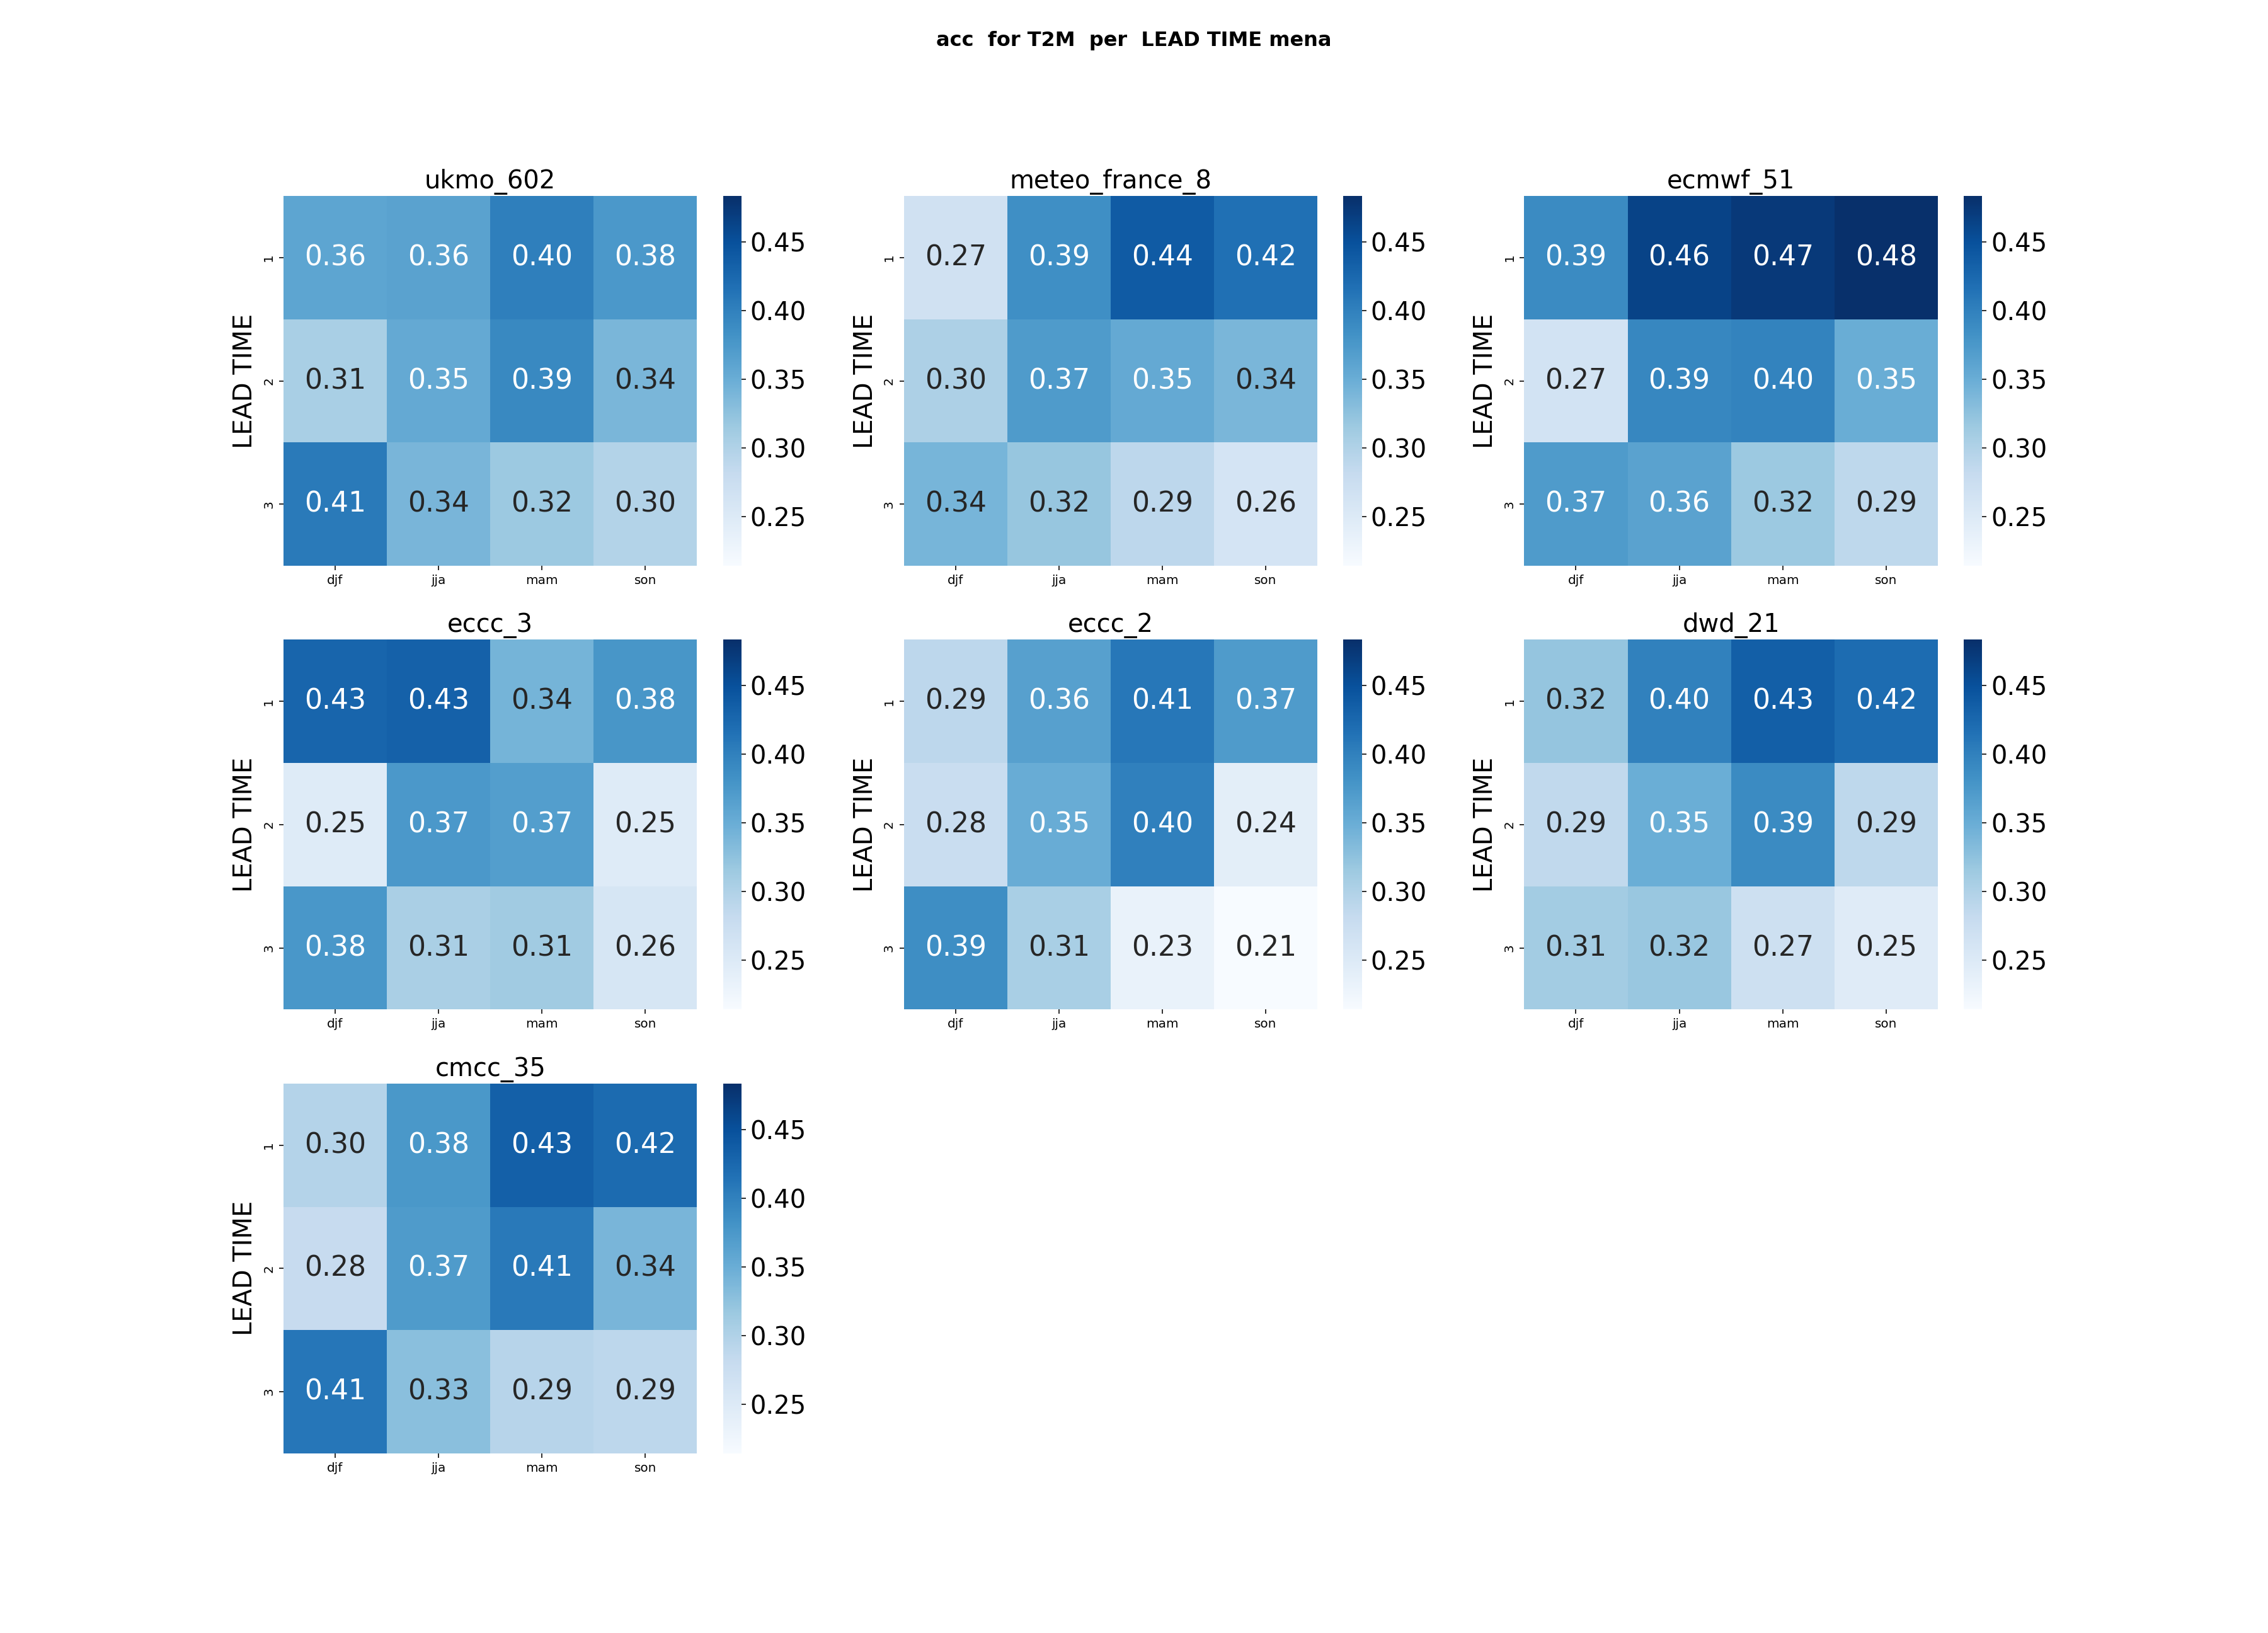
\includegraphics[scale=0.25]{plots/det/acc/acc_T2M_mena.png}
	\caption{The Heatmap of acc for the mena region for every period \textbf{\textit{(1 for perfect ACC)} }}
\end{figure}
The acc is moderate for all centers; however, the best models are \textbf{\textit{ECMWF, meteo-france and eccc-3}}. There is no clear variability in performance over time. For SON and JJA, performance is good at time 1 for all centers but decreases with increasing lead-time. Then, for DJF, \textbf{\textit{UKMO,ECCC-3 and ECMWF}} are the best with values between 0.39 and 0.43 for the first led-time and a little decrease along lead-time, the \textbf{\textit{CMCC-35}} show good acc with a value of 0.41 for the 3d lead-time. Moreover, for MAM and SON, we have good acc for the 1st lead-time, especially \textbf{\textit{ECMWF, METEO-FRANCE, DWD and CMCC-35}}, with values between 0.42 and 0.48, but this performance decrease greatly along lead-time to reach values around 0.2. The JJA show good and stable ACC for all centers and lead-times with values between 0.43 and 0.31. 

\begin{figure}[H]
	\centering
	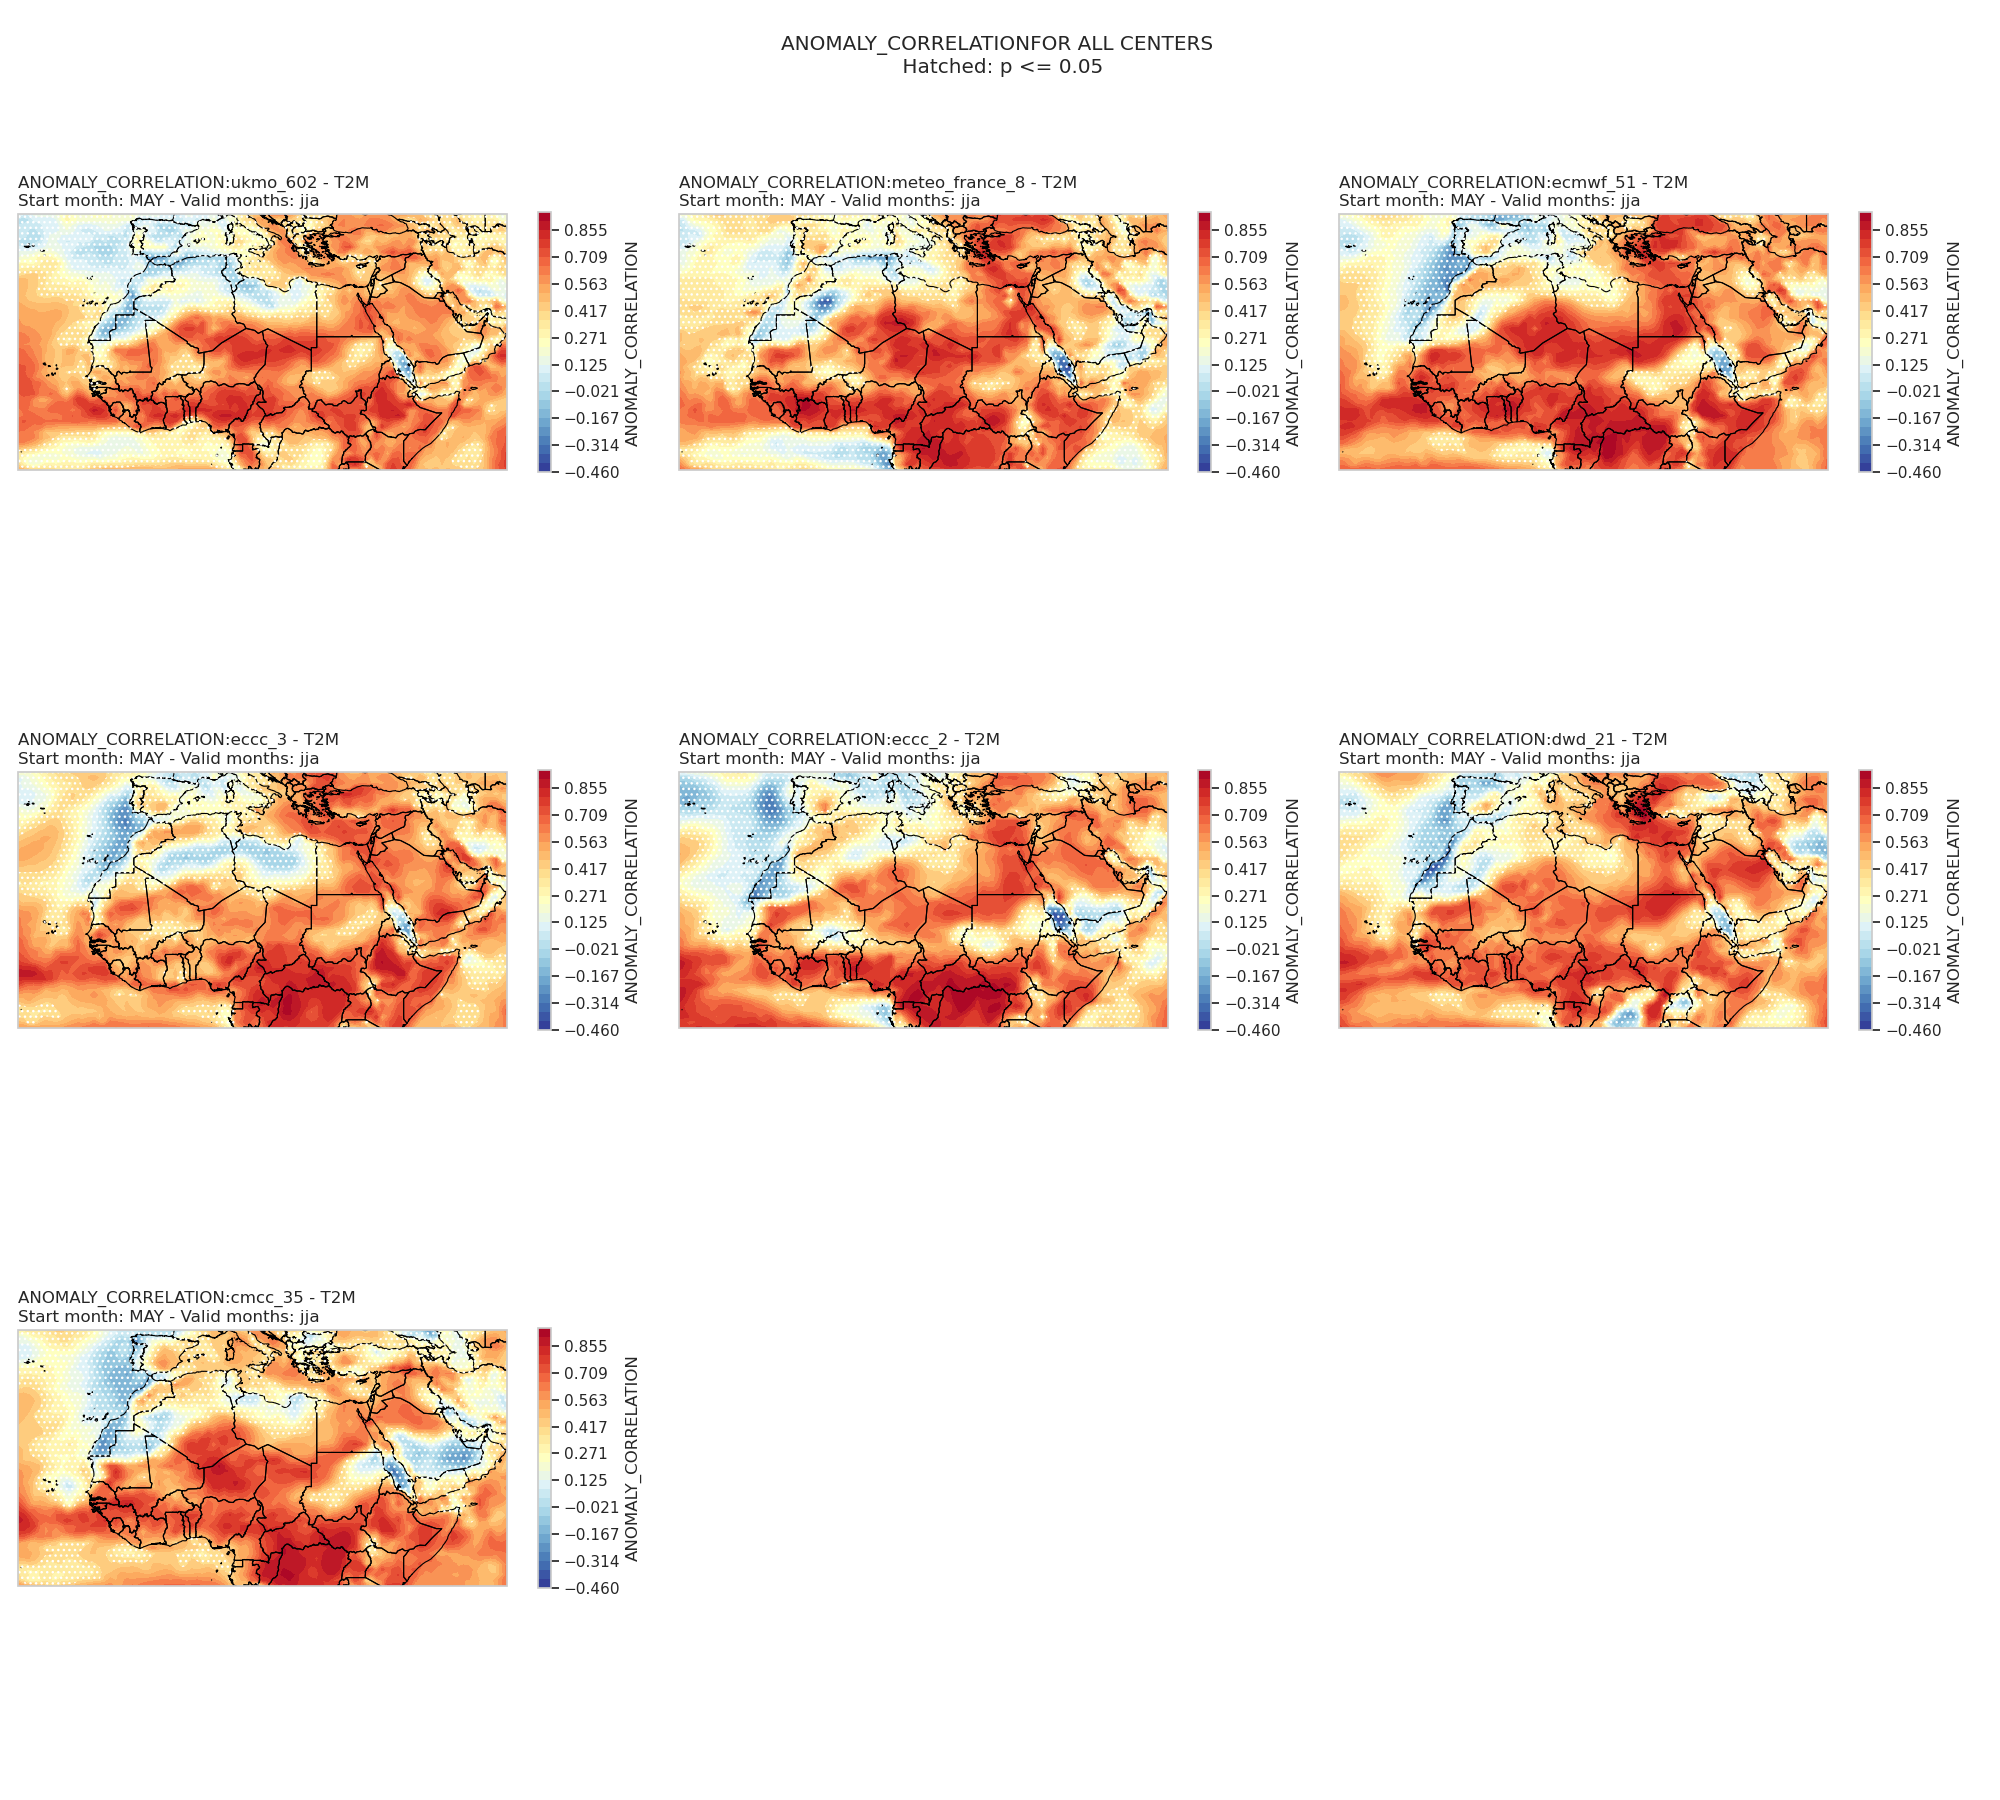
\includegraphics[scale=0.25]{plots/det/acc/ANOMALY_CORRELATION_jja_t2m.png}
	\caption{The 3 month rolling mean of JJA for  ACC for the mena region \textbf{\textit{(1 for perfect ACC)} }}
\end{figure}

the ACC demonstrates strong performance across nearly the entire region, indicating that the model captures the spatial patterns of anomalies effectively. This suggests a high level of agreement between observed and predicted anomalies, reflecting the model's reliability in representing anomaly patterns. However, despite this strong performance in terms of anomaly correlation, the significance of these correlations is not consistent across all regions. Specifically, in the center of Africa and the Arabian Peninsula, the correlations are not statistically significant. This implies that while the model captures the general patterns of anomalies in these areas, the strength of the linear relationship between observed and predicted anomalies is weak or uncertain.

\paragraph{Focus on North Africa}  
The heatmap below reveals that the \textbf{\textit{ECMWF}}, \textbf{\textit{UKMO}}, and \textbf{\textit{ECCC-3}} models demonstrate relatively strong correlations over the North Africa region. This suggests that these models perform well in capturing the anomalies in this specific area.  

\begin{figure}[H]
\centering
\includegraphics[scale=0.25]{plots/det/acc/acc_T2M_NorthAfrica.png}
\caption{ACC heatmap for the North Africa region across different periods.}
\end{figure}

\paragraph{Focus on the Arabian Peninsula}  
The heatmap for the Arabian Peninsula indicates strong performance across all forecasting centers, with \textbf{\textit{ECMWF}}, \textbf{\textit{UKMO}}, and \textbf{\textit{DWD}} exhibiting the highest correlation scores.  

\begin{figure}[H]
\centering
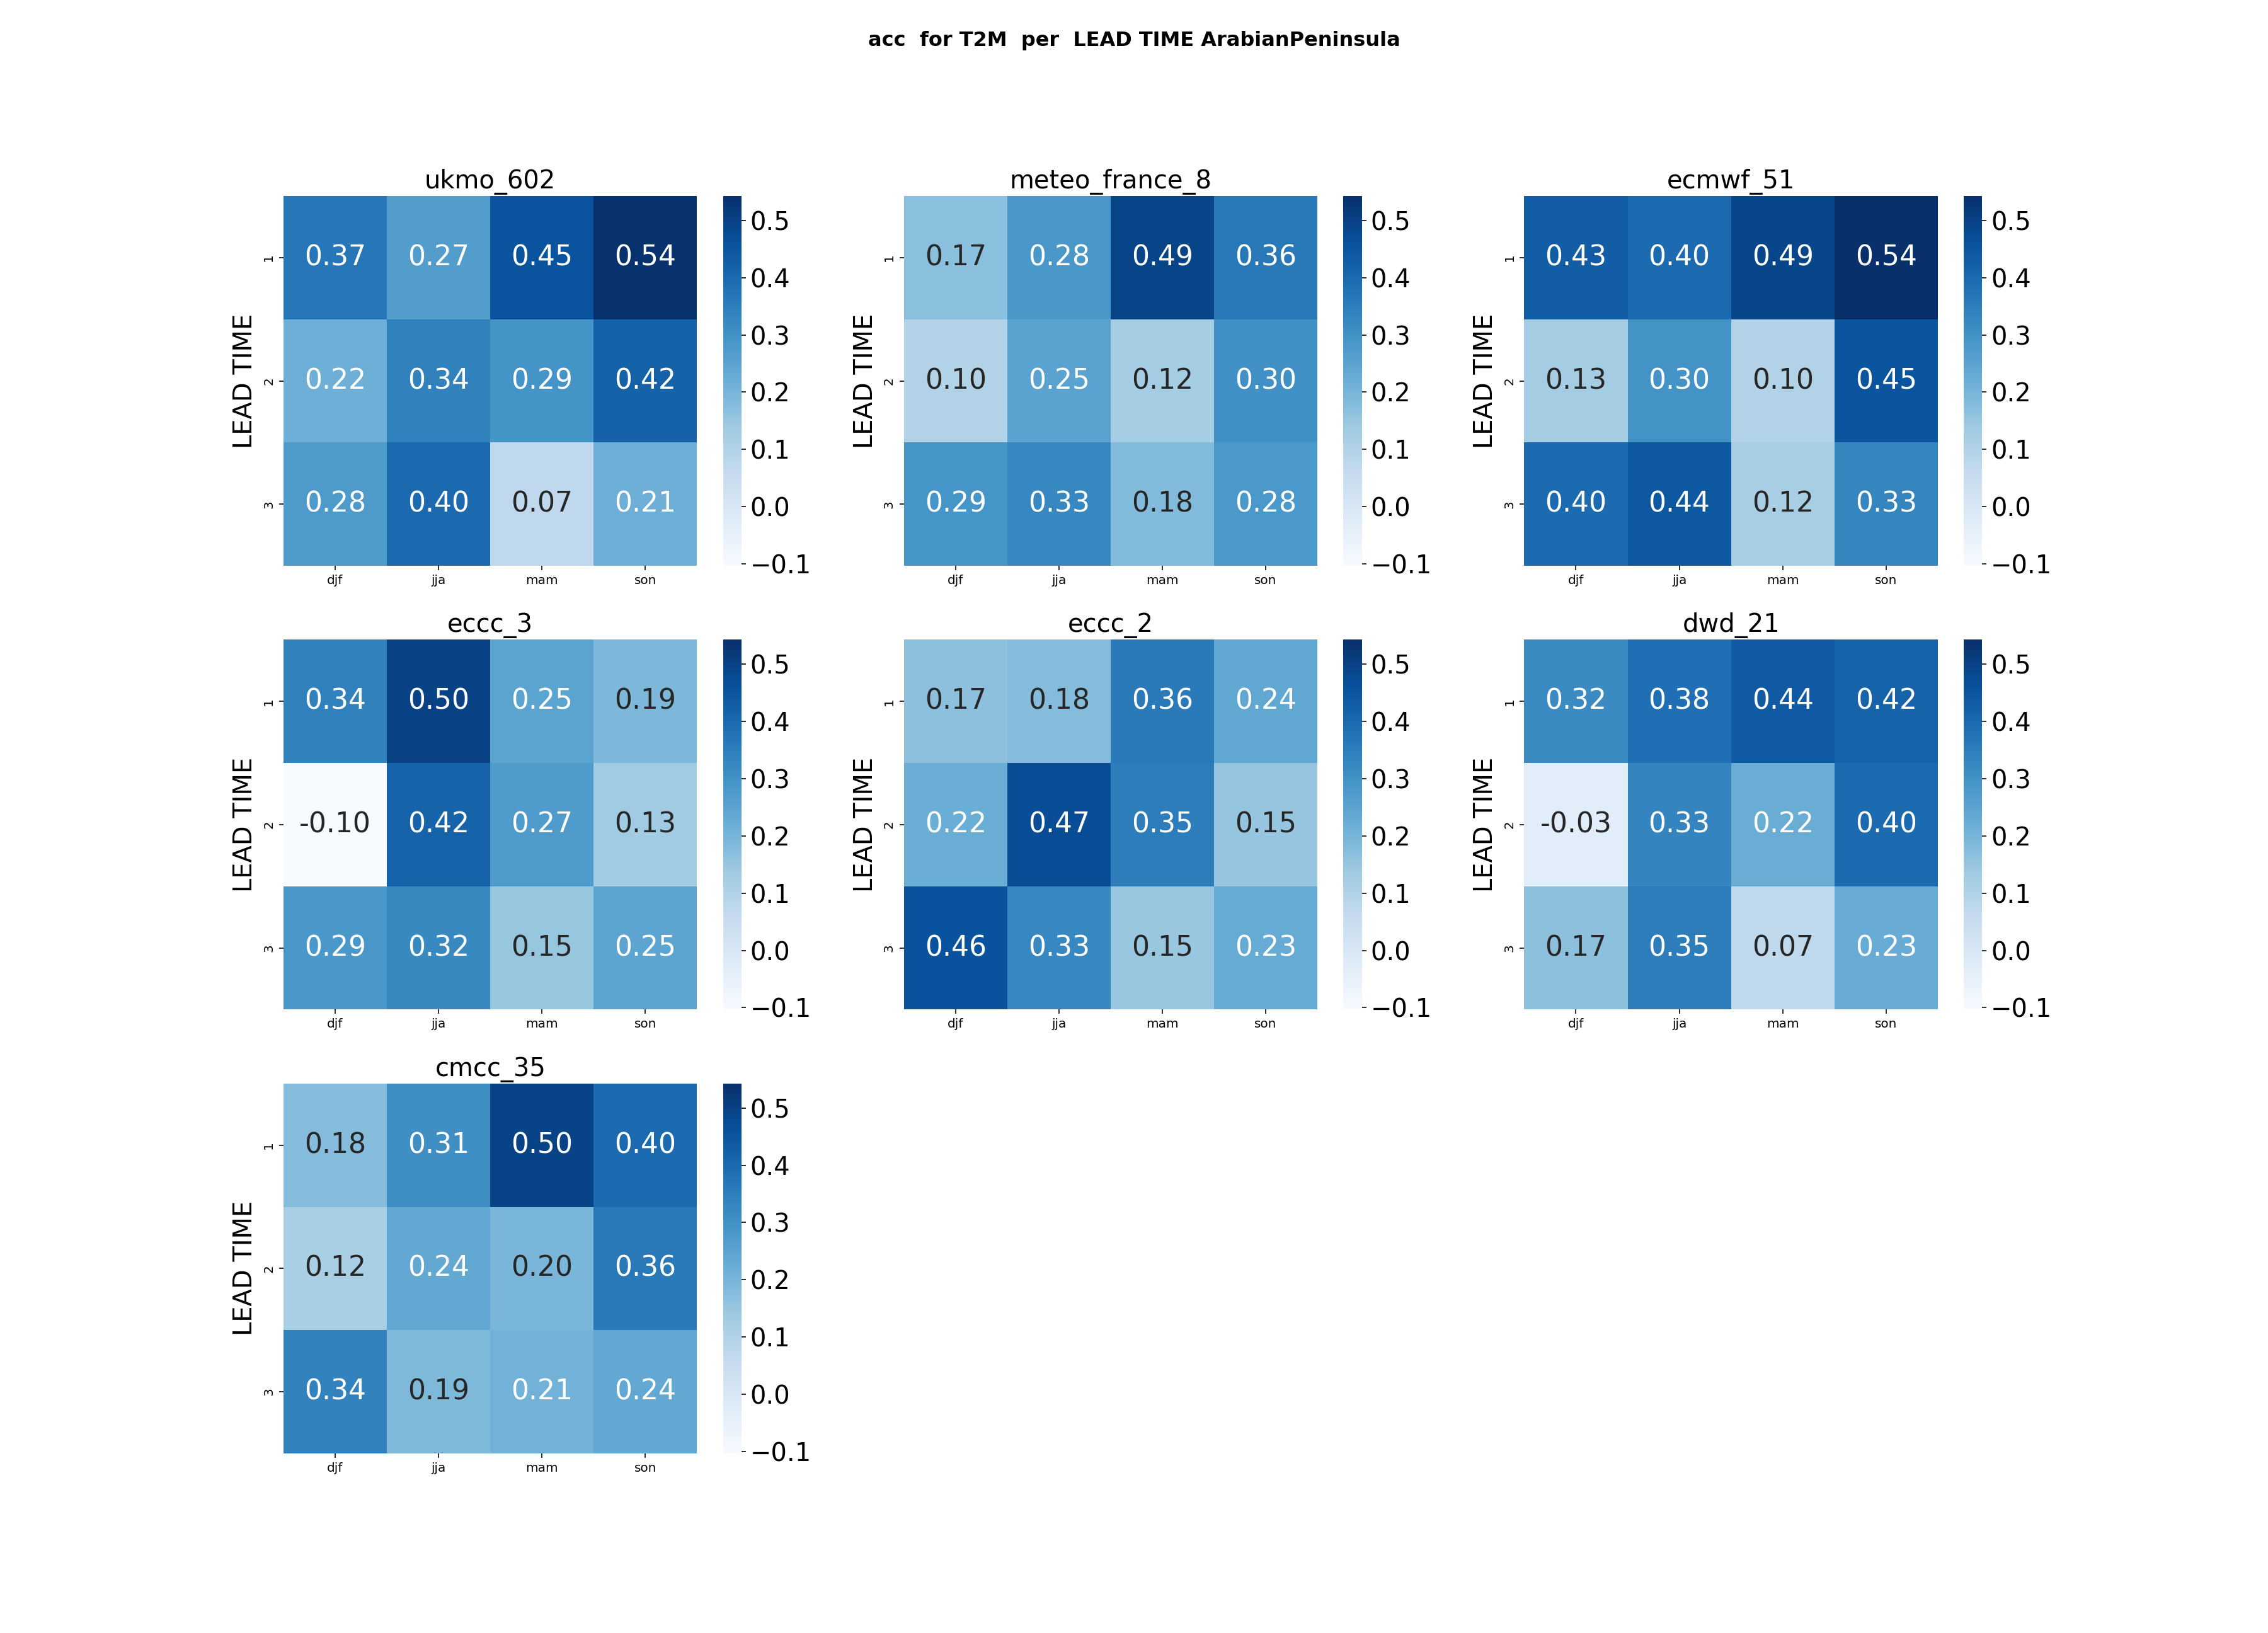
\includegraphics[scale=0.25]{plots/det/acc/acc_T2M_ArabianPeninsula.png}
\caption{ACC heatmap for the Arabian Peninsula across different periods \textbf{\textit{(1 indicates perfect correlation)}}.}
\end{figure}

The analysis highlights that the Arabian Peninsula consistently achieves better ACC scores compared to the general MENA region. Notably, the ACC is particularly high for \textbf{\textit{SON (September-October-November)}} at the third lead time.
\subsubsection{Root Mean Square Error}


The maps in this section show the RMSE (Root Mean Square Error) between observed and modeled surface temperatures across the MENA region for the four seasons: JJA, DJF, MAM, and SON. The RMSE, expressed in the same units as temperature, evaluates the accuracy of climate models, with lower values indicating better performance.  These maps help identify the strengths and limitations of the models across seasons, contributing to the improvement of climate forecasts for the region.
\begin{figure}[H]
    \centering
    \includegraphics[width=1\linewidth]{plots/det/rmse/rmse_T2M.png}
    \caption{Temperature rmse heatmaps for all the sasons \textbf{\textit{(0 for perfect RMSE)} }}
\end{figure}

The heatmap for the seven models highlights distinct variations in their seasonal performance. The UKMO model shows moderate to good performance, particularly in JJA and MAM, as reflected by relatively low RMSE values ranging between 1.35°C and 1.51°C across the three lead times. This indicates that the UKMO model is reasonably effective in capturing surface temperature variations during these seasons, likely benefiting from its ability to simulate key atmospheric processes during these periods.

In contrast, Météo-France exhibits weaker performance in JJA, with higher RMSE values suggesting less accurate predictions of surface temperatures during this season. This could be attributed to the model's limitations in capturing summer-specific temperature drivers in the MENA region, such as heatwaves, desert-air interactions, or seasonal atmospheric circulation patterns.

The ECMWF model emerges as the best-performing model based on the heatmap, particularly during JJA, where it demonstrates high predictive accuracy and consistency. This is supported by the RMSE map, which shows significantly lower RMSE values across most of the MENA region. These low RMSE values confirm the ECMWF model's ability to capture regional temperature dynamics effectively, with reduced errors across diverse climatic zones.

Notably, the spatial distribution of RMSE on the map reinforces the ECMWF's strong performance, as it maintains relatively low error values in critical parts of the MENA region. This suggests that the ECMWF model is better equipped to account for the complex climatic interactions in the region, such as the influence of desert regions, coastal temperature gradients, and seasonal weather patterns.

Overall, these findings emphasize the importance of selecting climate models based on their seasonal and spatial performance, as they play a critical role in improving the accuracy of temperature forecasts for the MENA region.



\begin{figure}[H]
    \centering
    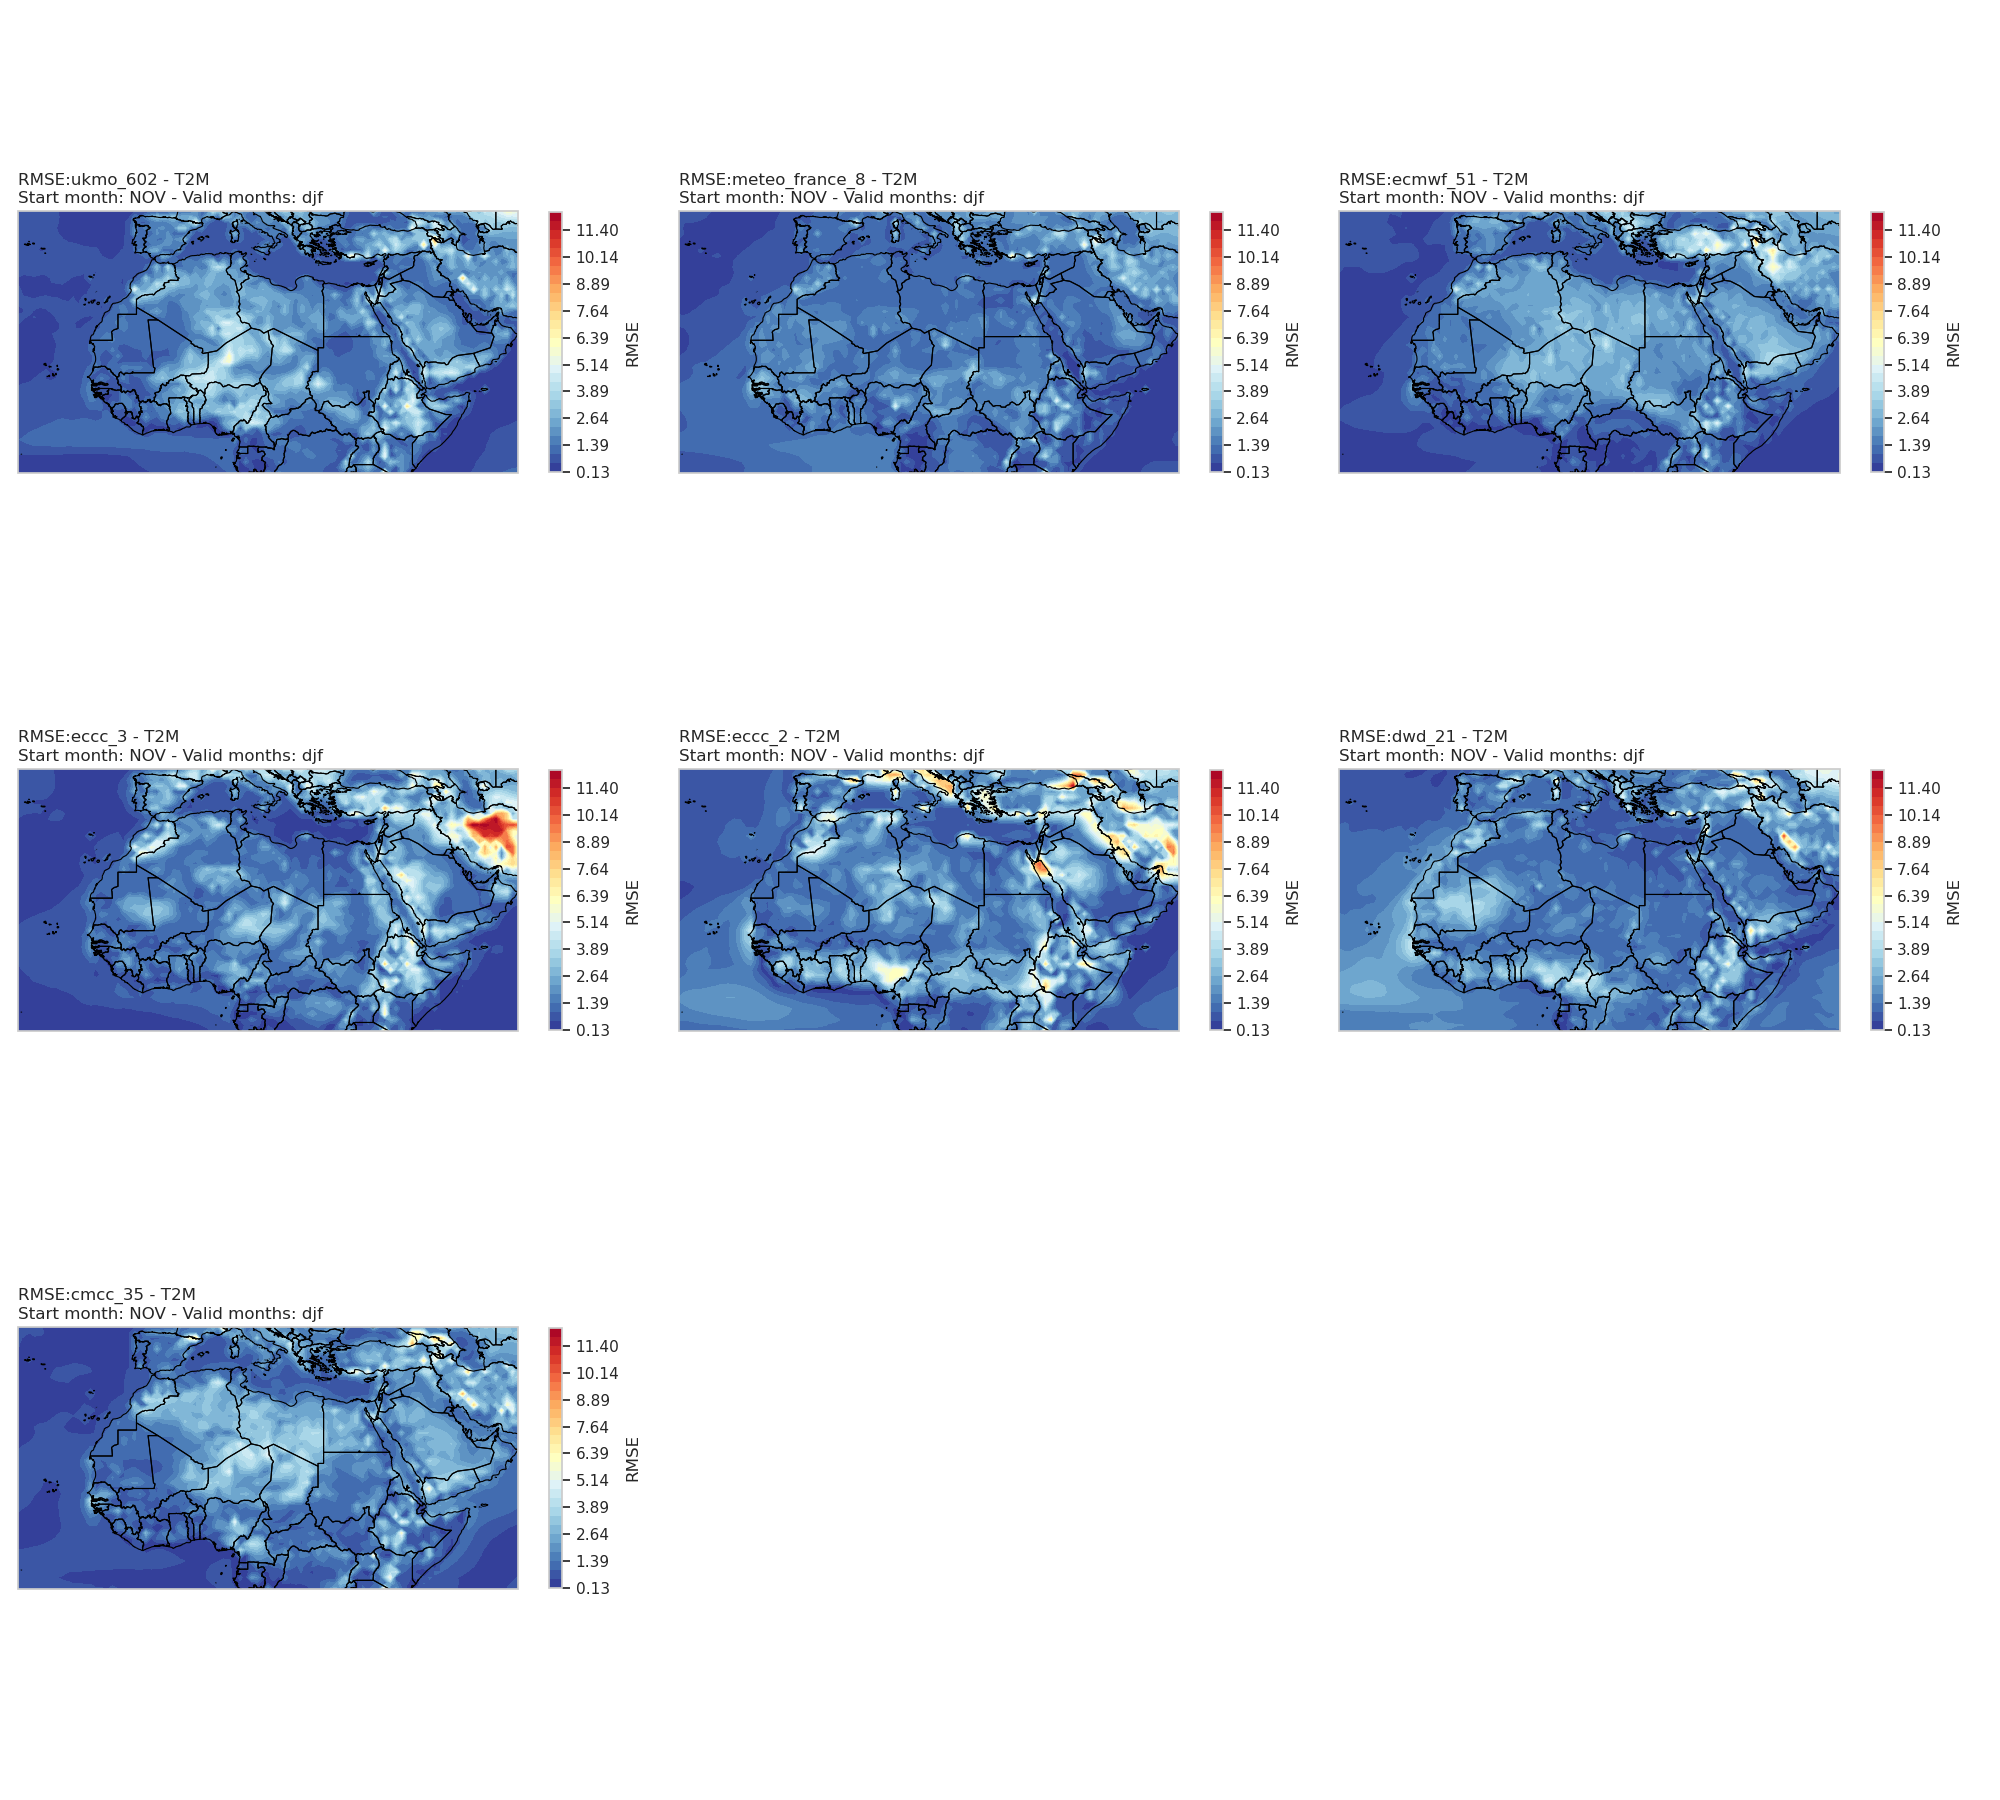
\includegraphics[width=1\linewidth]{plots/det/rmse/rmse_djf_t2m.png}
    \caption{The 3 month rolling mean of Temperature rmse for DJF for all centers \textbf{\textit{(0 for perfect RMSE)} }}
\end{figure}

The analysis of the RMSE highlights several key patterns. Overall, most regions exhibit low RMSE values, indicating a good agreement between the hindcast and observations and suggesting strong model performance across a large portion of the domain. Central and western Africa consistently show low RMSE across all models, reflecting robust forecasting accuracy in these regions. However, variations are evident in northern Africa, particularly in the Sahara, where some areas experience moderate discrepancies depending on the model. The Arabian Peninsula also stands out with localized regions of higher RMSE, especially in its northern parts, suggesting challenges in these areas. Among the models, the UKMO, Météo-France, and ECMWF generally perform well, with ECMWF demonstrating consistent low RMSE across the entire domain. In contrast, the ECCC-3 and ECCC-2 models exhibit higher RMSE in specific areas, such as northern Africa and the Arabian Peninsula, while the DWD model performs comparably to the best models in most regions. 
\paragraph{focus on North Africa} : 
\begin{figure}[H]
\centering
\includegraphics[scale=0.3]{plots/det/rmse/rmse_T2M_NorthAfrica.png}
\caption{heatmap of RMSE For T2M  (North Africa)}
\end{figure}

The North African climate poses challenges for modeling extreme temperatures and spatial variability. Heatmap analysis shows that \textbf{\textit{ECMWF}} excels in JJA with RMSE values of 1.34°C–1.58°C but performs lower in other seasons. \textbf{\textit{Météo-France}} delivers consistent accuracy, especially in SON, making it more reliable for multi-seasonal forecasting in this region.
\vspace{1.5cm}
\paragraph{focus on Arabian Peninsula}:

\begin{figure}[H]
\centering
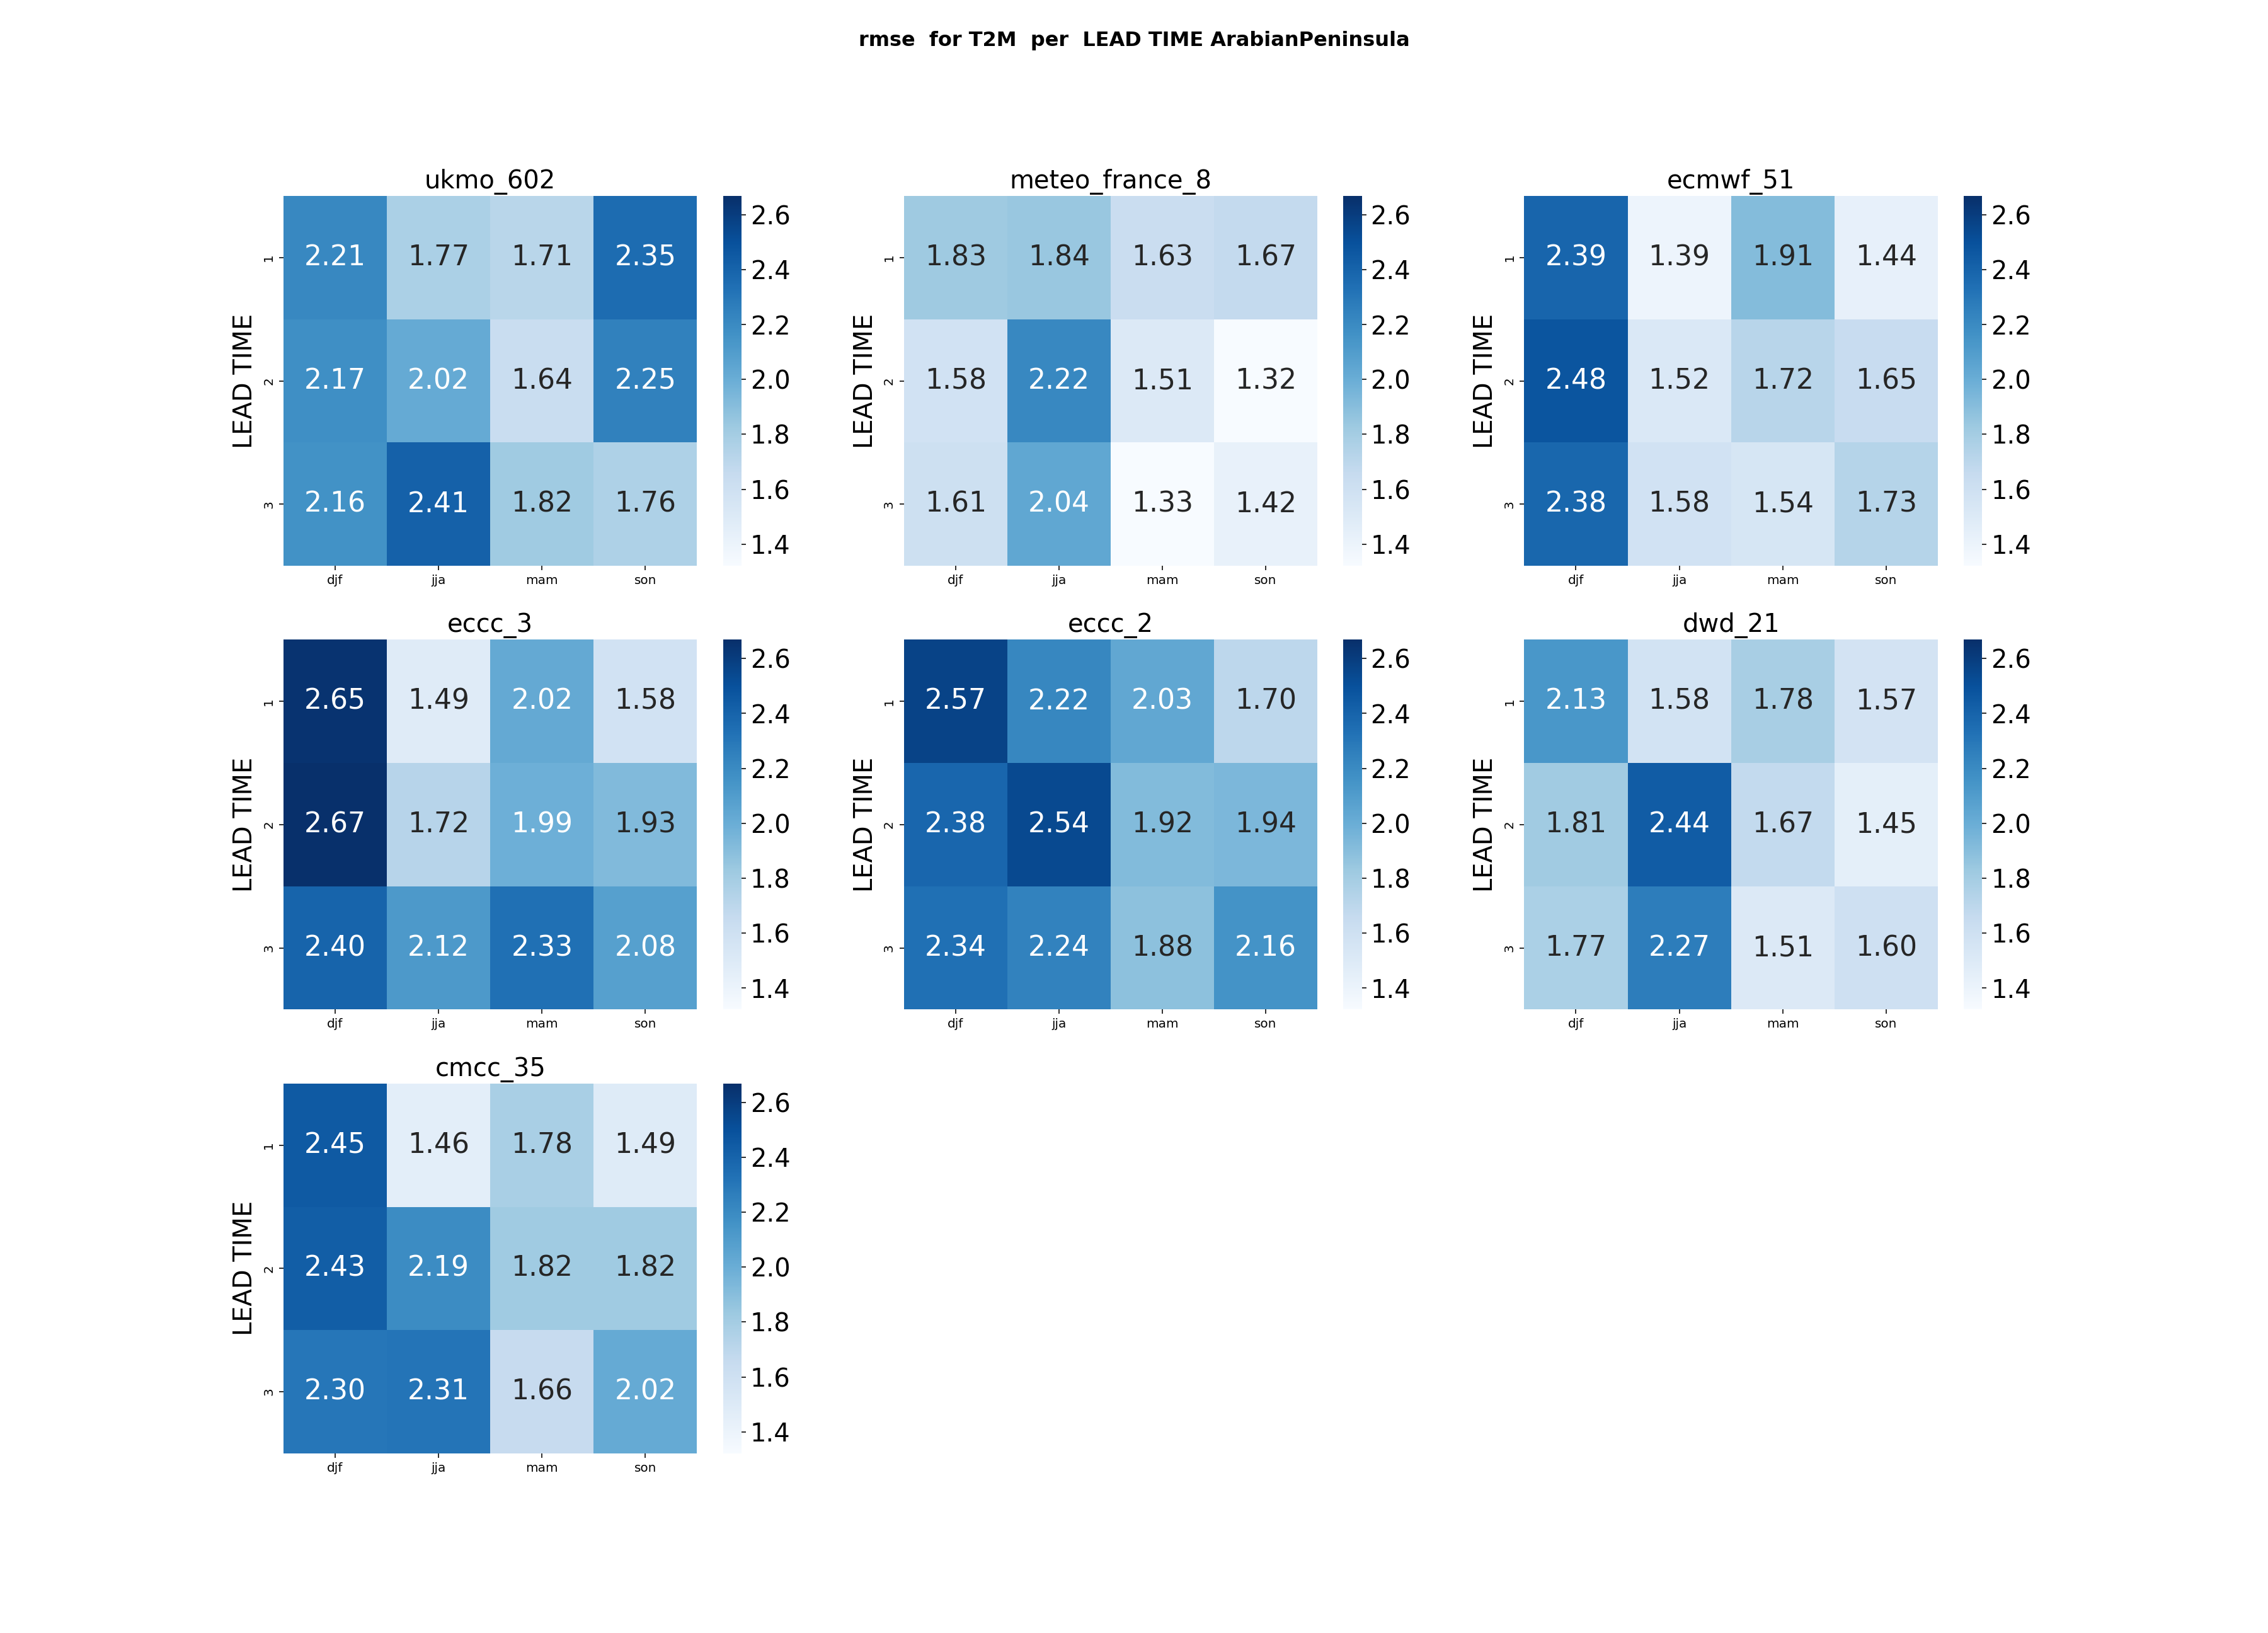
\includegraphics[scale=0.3]{plots/det/rmse/rmse_T2M_ArabianPeninsula.png}
\caption{heatmap of RMSE For T2M  (Arabian Peninsula)}
\end{figure}

In the same way as North Africa, the RMSE for the Arabian Peninsula is significantly lower for \textbf{\textit{Météo-France}}, indicating superior performance.
\subsubsection{coefficient of determination}


The maps in this section show the Rsquared between observed and modeled surface temperatures across the MENA region for the four seasons: JJA, DJF, MAM, and SON. R-squared is a statistical measure that indicates how well the model explains the variability in observed data, with values closer to 1 signifying better performance. These maps provide valuable insights into the predictive skill of the climate models, highlighting their ability to capture seasonal temperature patterns.

\begin{figure}[H]
    \centering
    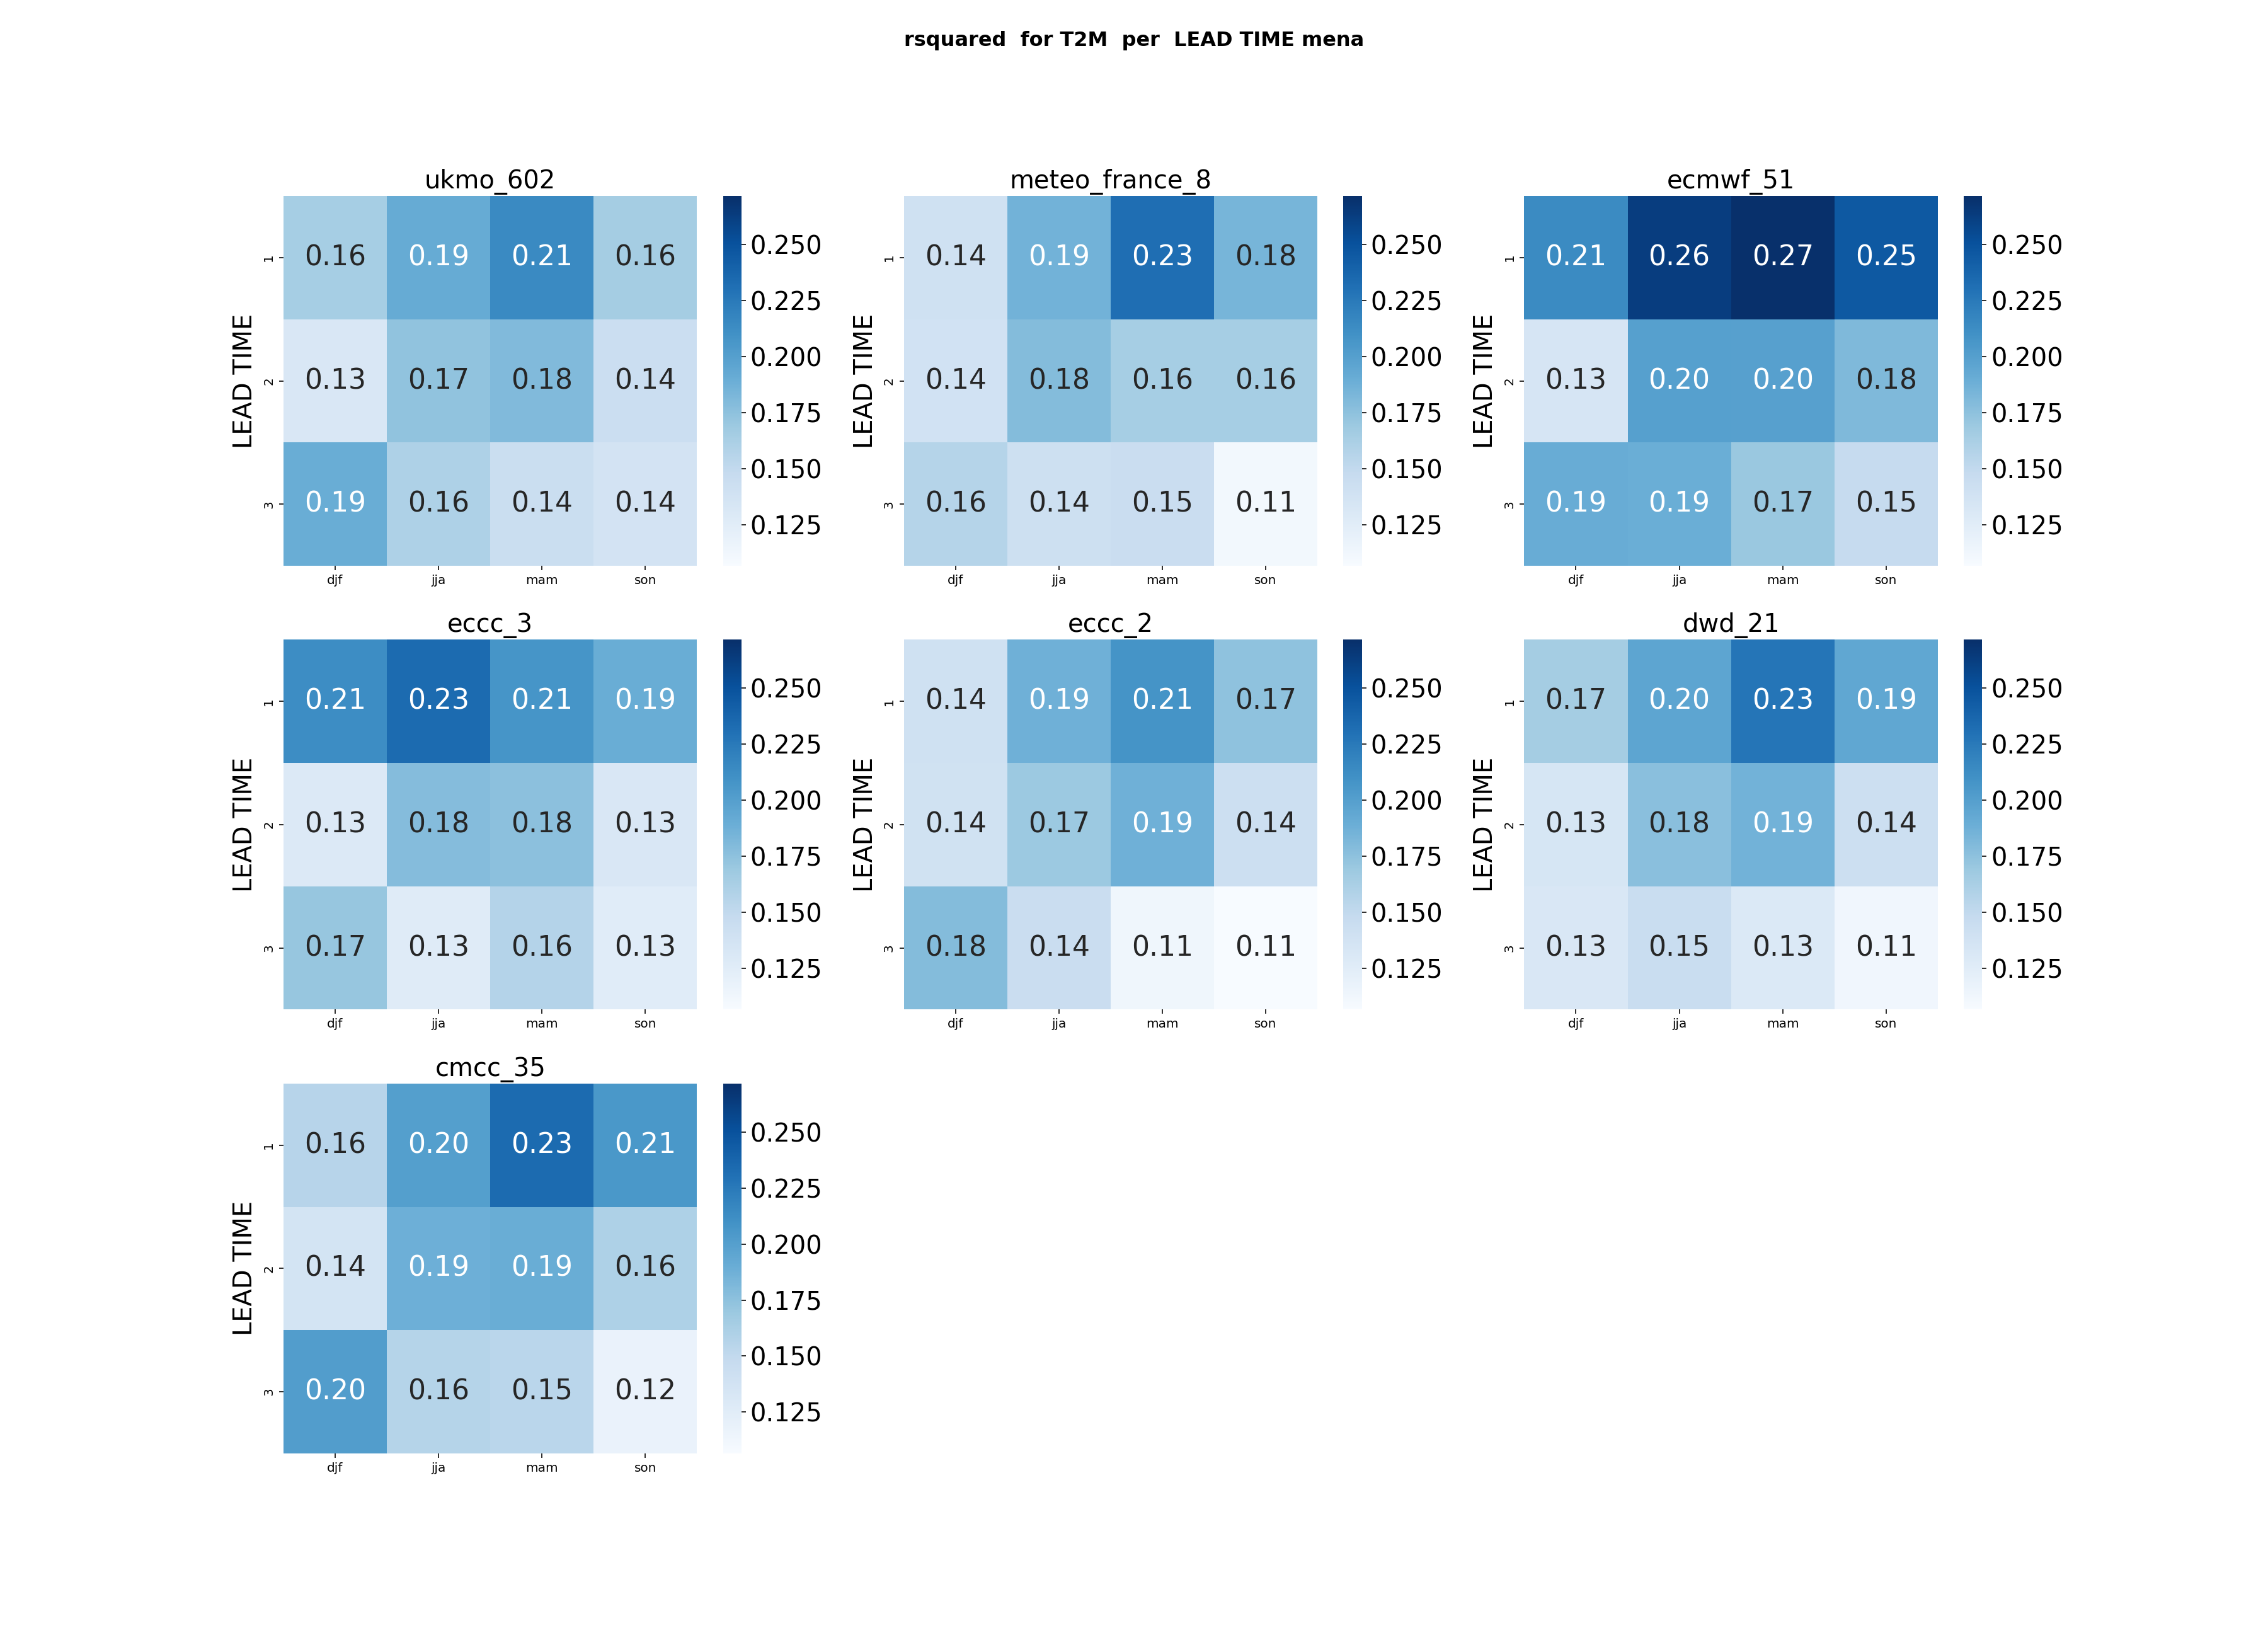
\includegraphics[width=1\linewidth]{plots/det/rsquared/rsquared_T2M_mena.png}
    \caption{Temperature rsquared heatmaps for all the seasons \textbf{\textit{(1 for perfect R-SQUARED)} }}
\end{figure}
Based on this deterministic metric (R-squared), the ECMWF model demonstrates superior performance for lead time 1 across all four seasons, particularly during MAM. In general, the portion of variance explained by the model decreases as the lead time increases. This indicates that while the model is highly effective at capturing seasonal variability of surface temperatures in the short term, its predictive skill diminishes over longer time horizons.

The strong performance during MAM highlights the ECMWF model’s ability to capture the complexities of spring, a season marked by transitional weather patterns in the MENA region. The high R-squared values during this period suggest that the model accurately reflects observed temperature variability by effectively simulating key drivers such as the gradual warming trend, atmospheric circulation changes, and the interaction between desert and coastal dynamics.

Such precision underscores the ECMWF model’s reliability for short-term seasonal forecasting, particularly during periods of heightened climatic variability like MAM. However, the decreasing performance with increasing lead times suggests the need for careful interpretation of forecasts beyond lead time 1, as uncertainty increases with longer projections.


\begin{figure}[H]
    \centering
    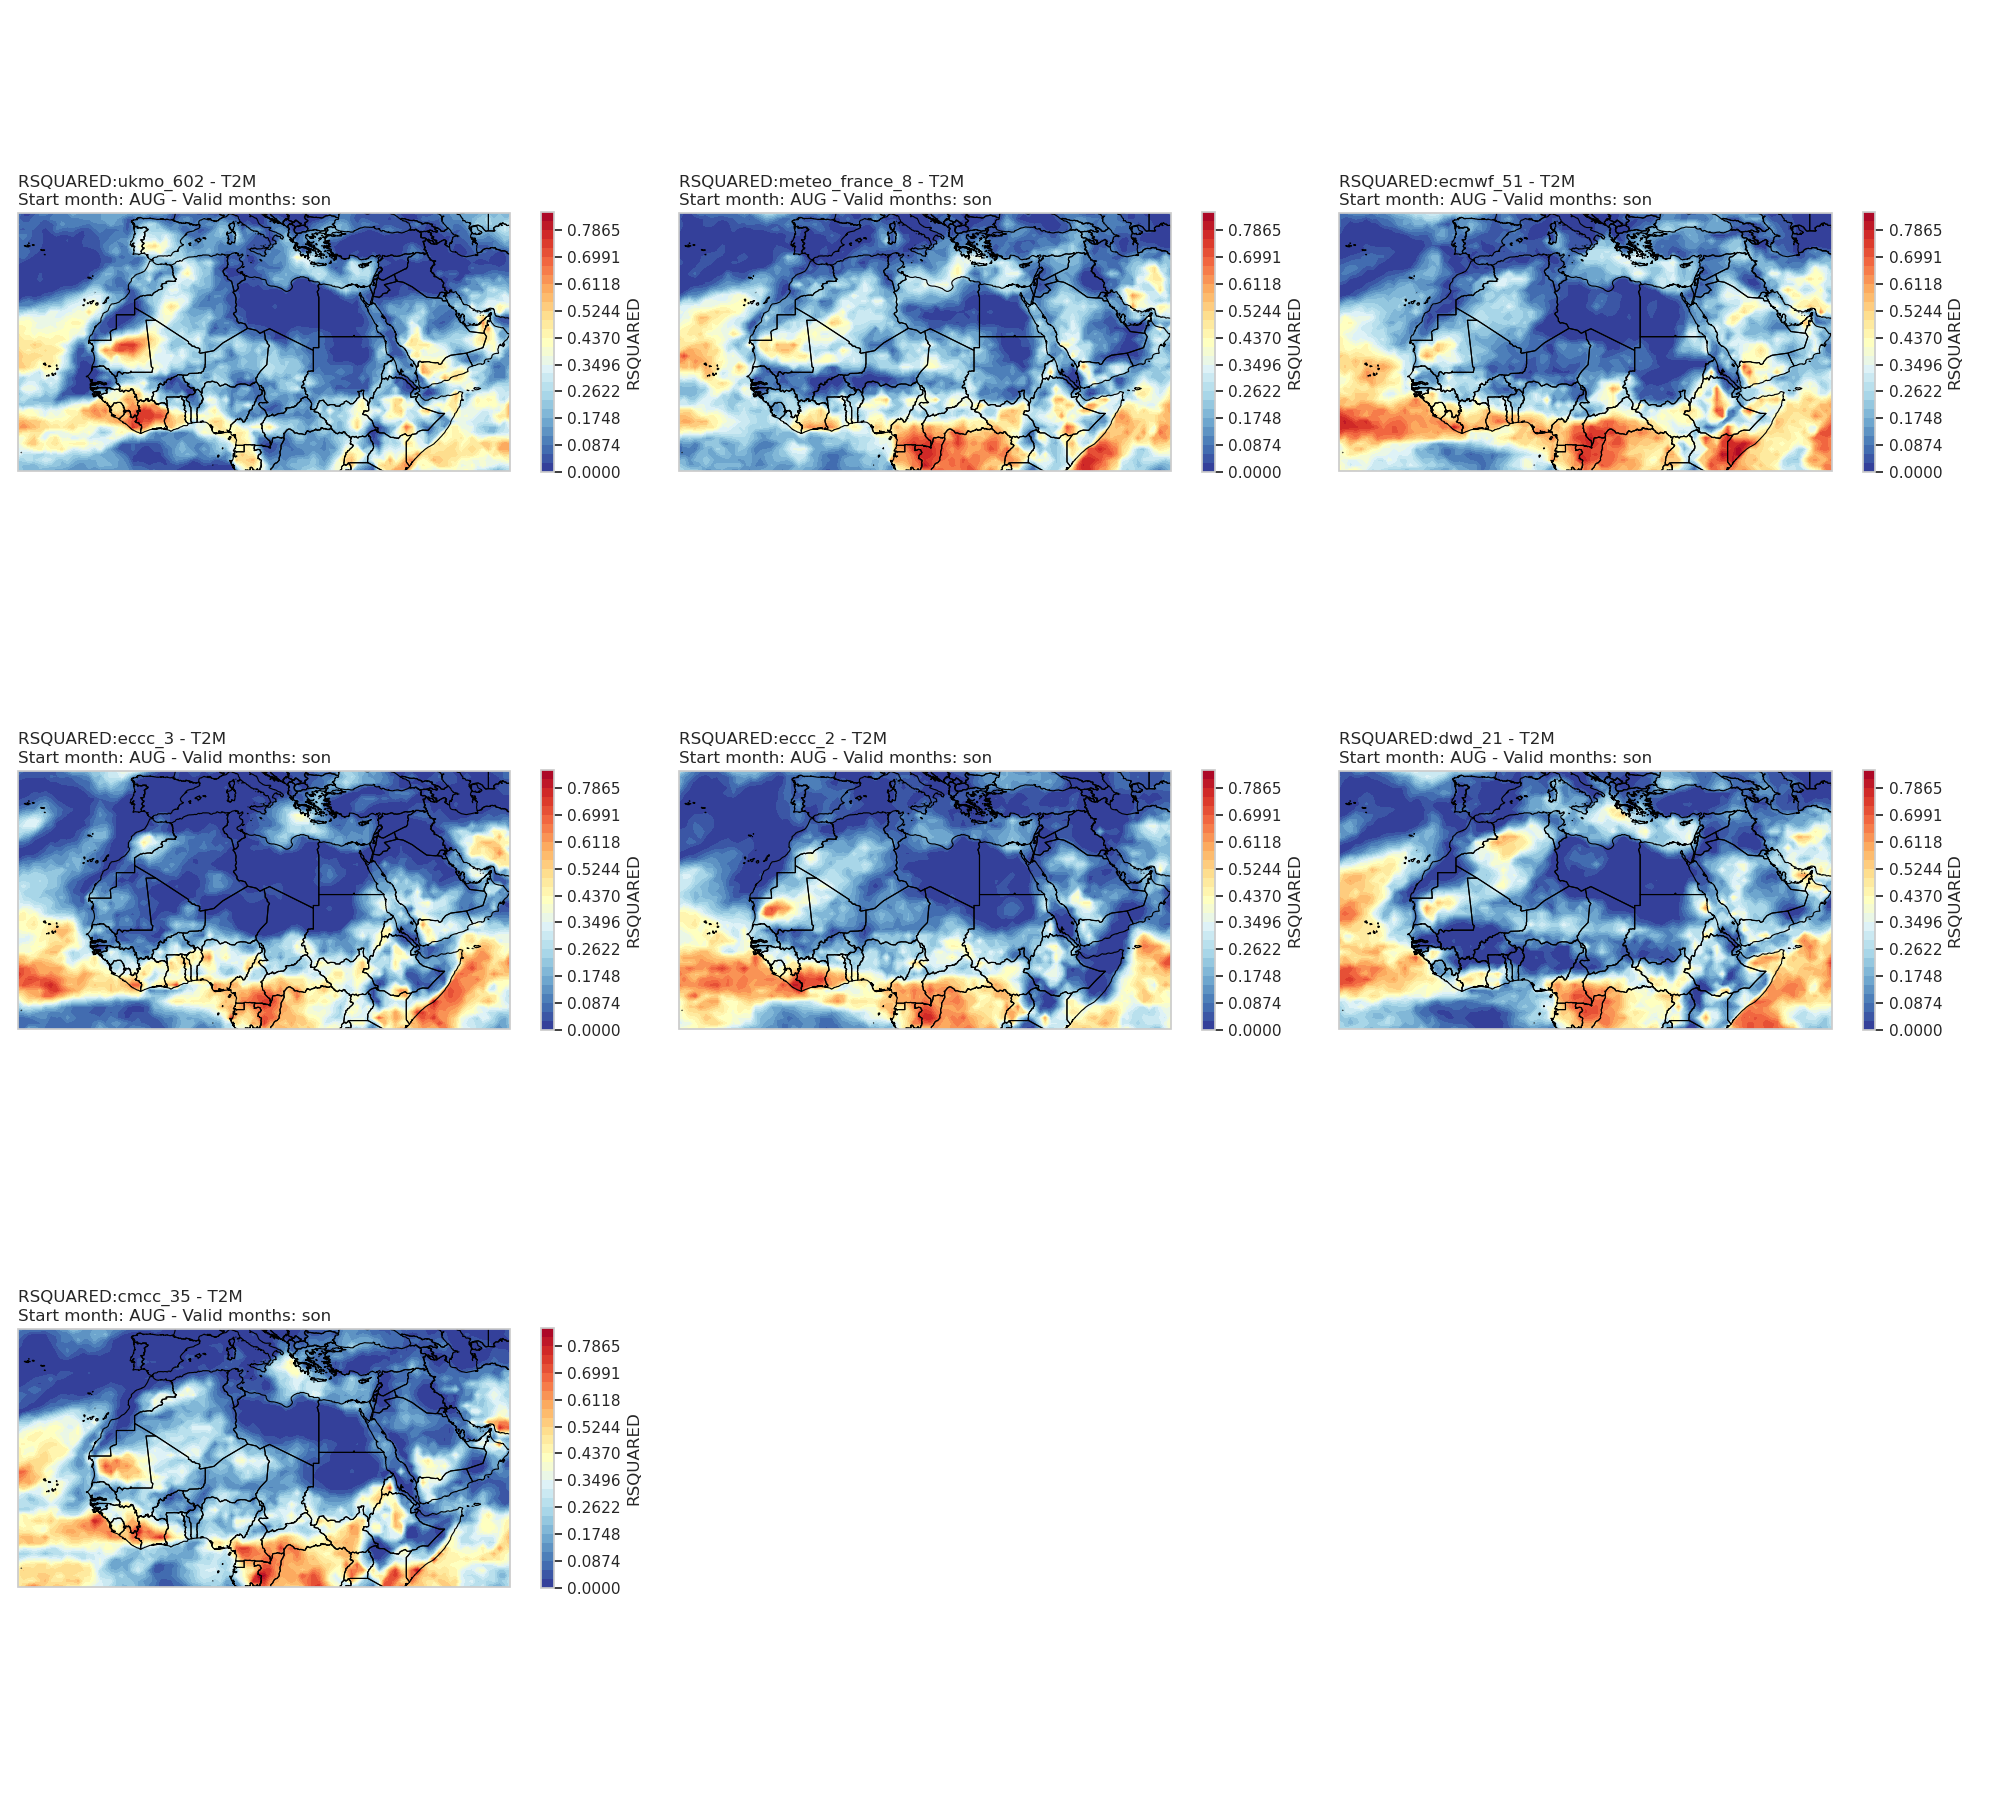
\includegraphics[width=1\linewidth]{plots/det/rsquared/rsquared_son_t2m.png}
    \caption{3-months rolling mean of 2-meter temperature of SON R-SQUARED  for all centers \textbf{\textit{(1 for perfect R-SQUARED)} }}
\end{figure}

From the figure above, the R-SQUARED is excellent at the equator, reaching a maximum value of 0.78. All the centers exhibit good R-SQUARED performance in this region; nevertheless, the ECMWF model demonstrates slightly better performance overall. Across the northern parts of Africa, the R-SQUARED values decrease, indicating a reduced agreement between the hindcast and observations. However, some models, such as Météo-France and ECCC-3, maintain moderate performance in certain localized areas. The Arabian Peninsula exhibits generally low R-SQUARED values across all models, signifying challenges in capturing seasonal variability in this region. The southern part of the domain, particularly over regions near Angola and Zambia, shows moderate R-SQUARED values in some models, such as UKMO and CMCC.

Thus, while the equatorial region consistently shows excellent performance across all models, northern Africa and the Arabian Peninsula represent areas with lower R-SQUARED values, highlighting potential limitations in the seasonal forecasting system. Among the models, ECMWF appears to have a slight advantage in terms of consistency and accuracy.
\paragraph{focus on North Africa}

Focusing on North Africa, \textbf{\textit{ECMWF}} maintains its position as the most reliable center, consistent with its performance across the broader MENA region.
\begin{figure}[H]
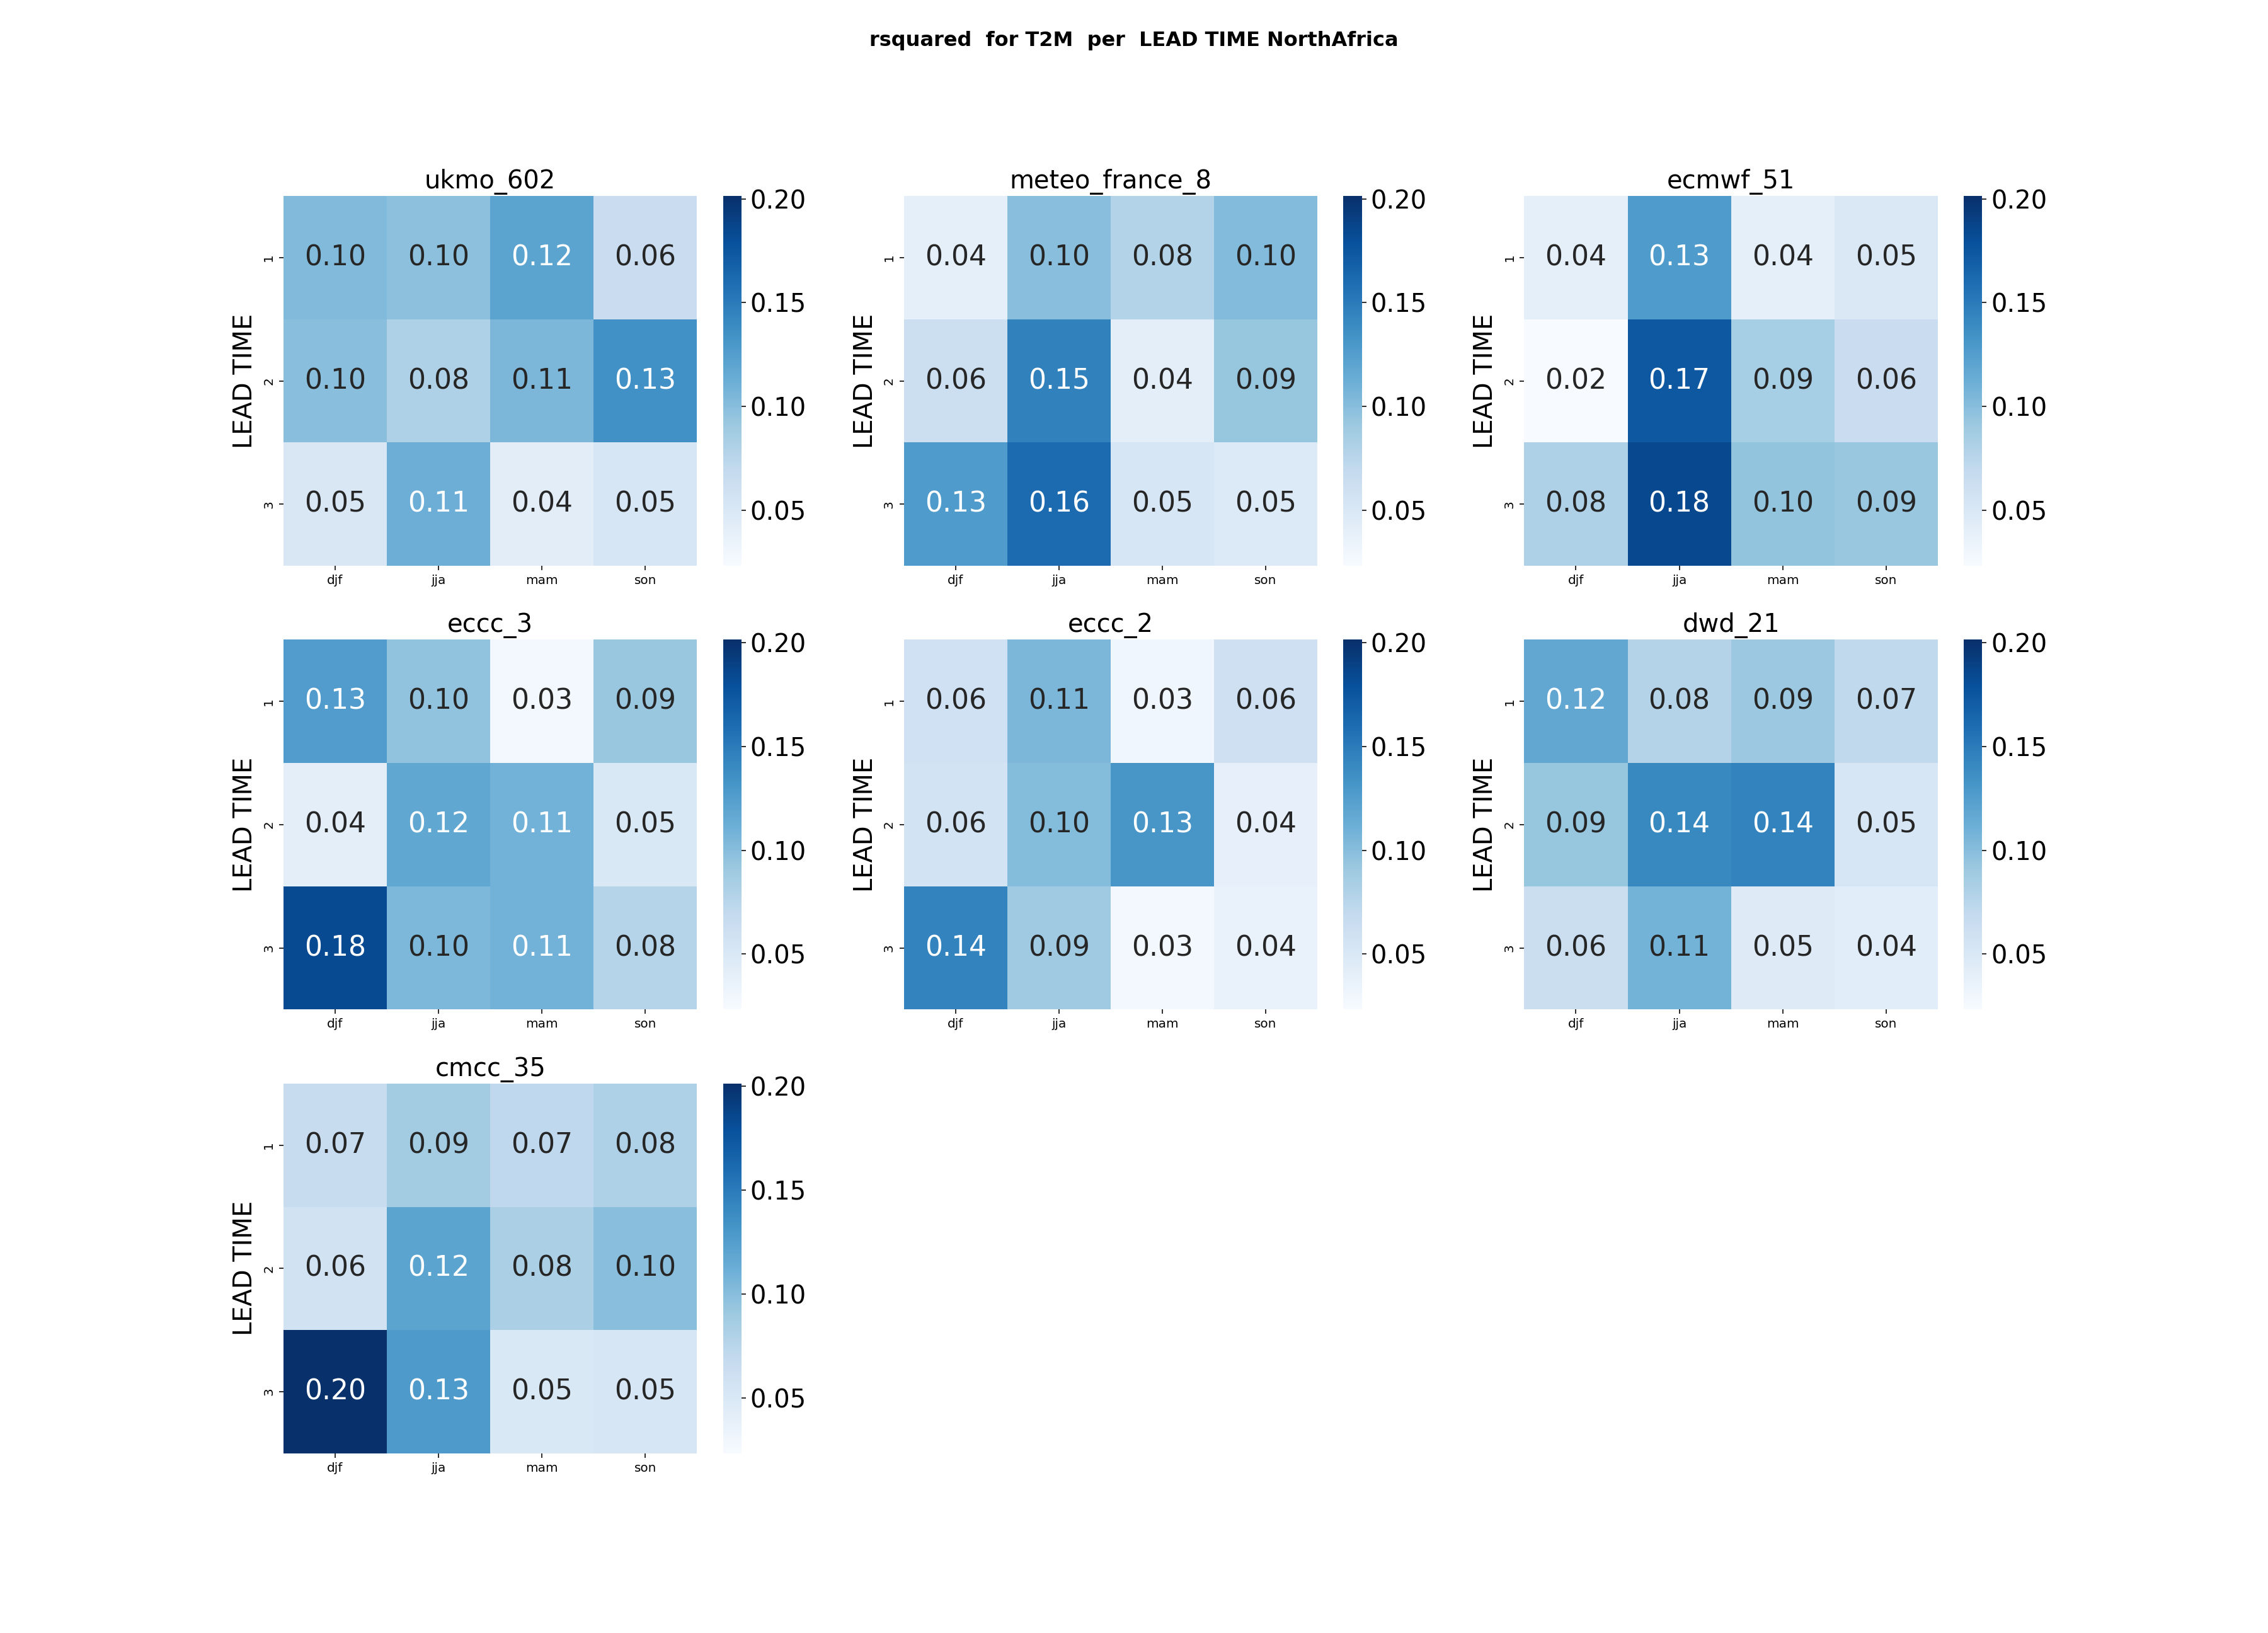
\includegraphics[scale=0.3]{plots/det/rsquared/rsquared_T2M_NorthAfrica.png}
\caption{Heatmap of T2M  RSQUARED in North Africa Region for all centers }
\end{figure}


\vspace{1.5cm}
\paragraph{focus on Arabian Peninsula}:


\begin{figure}[H]
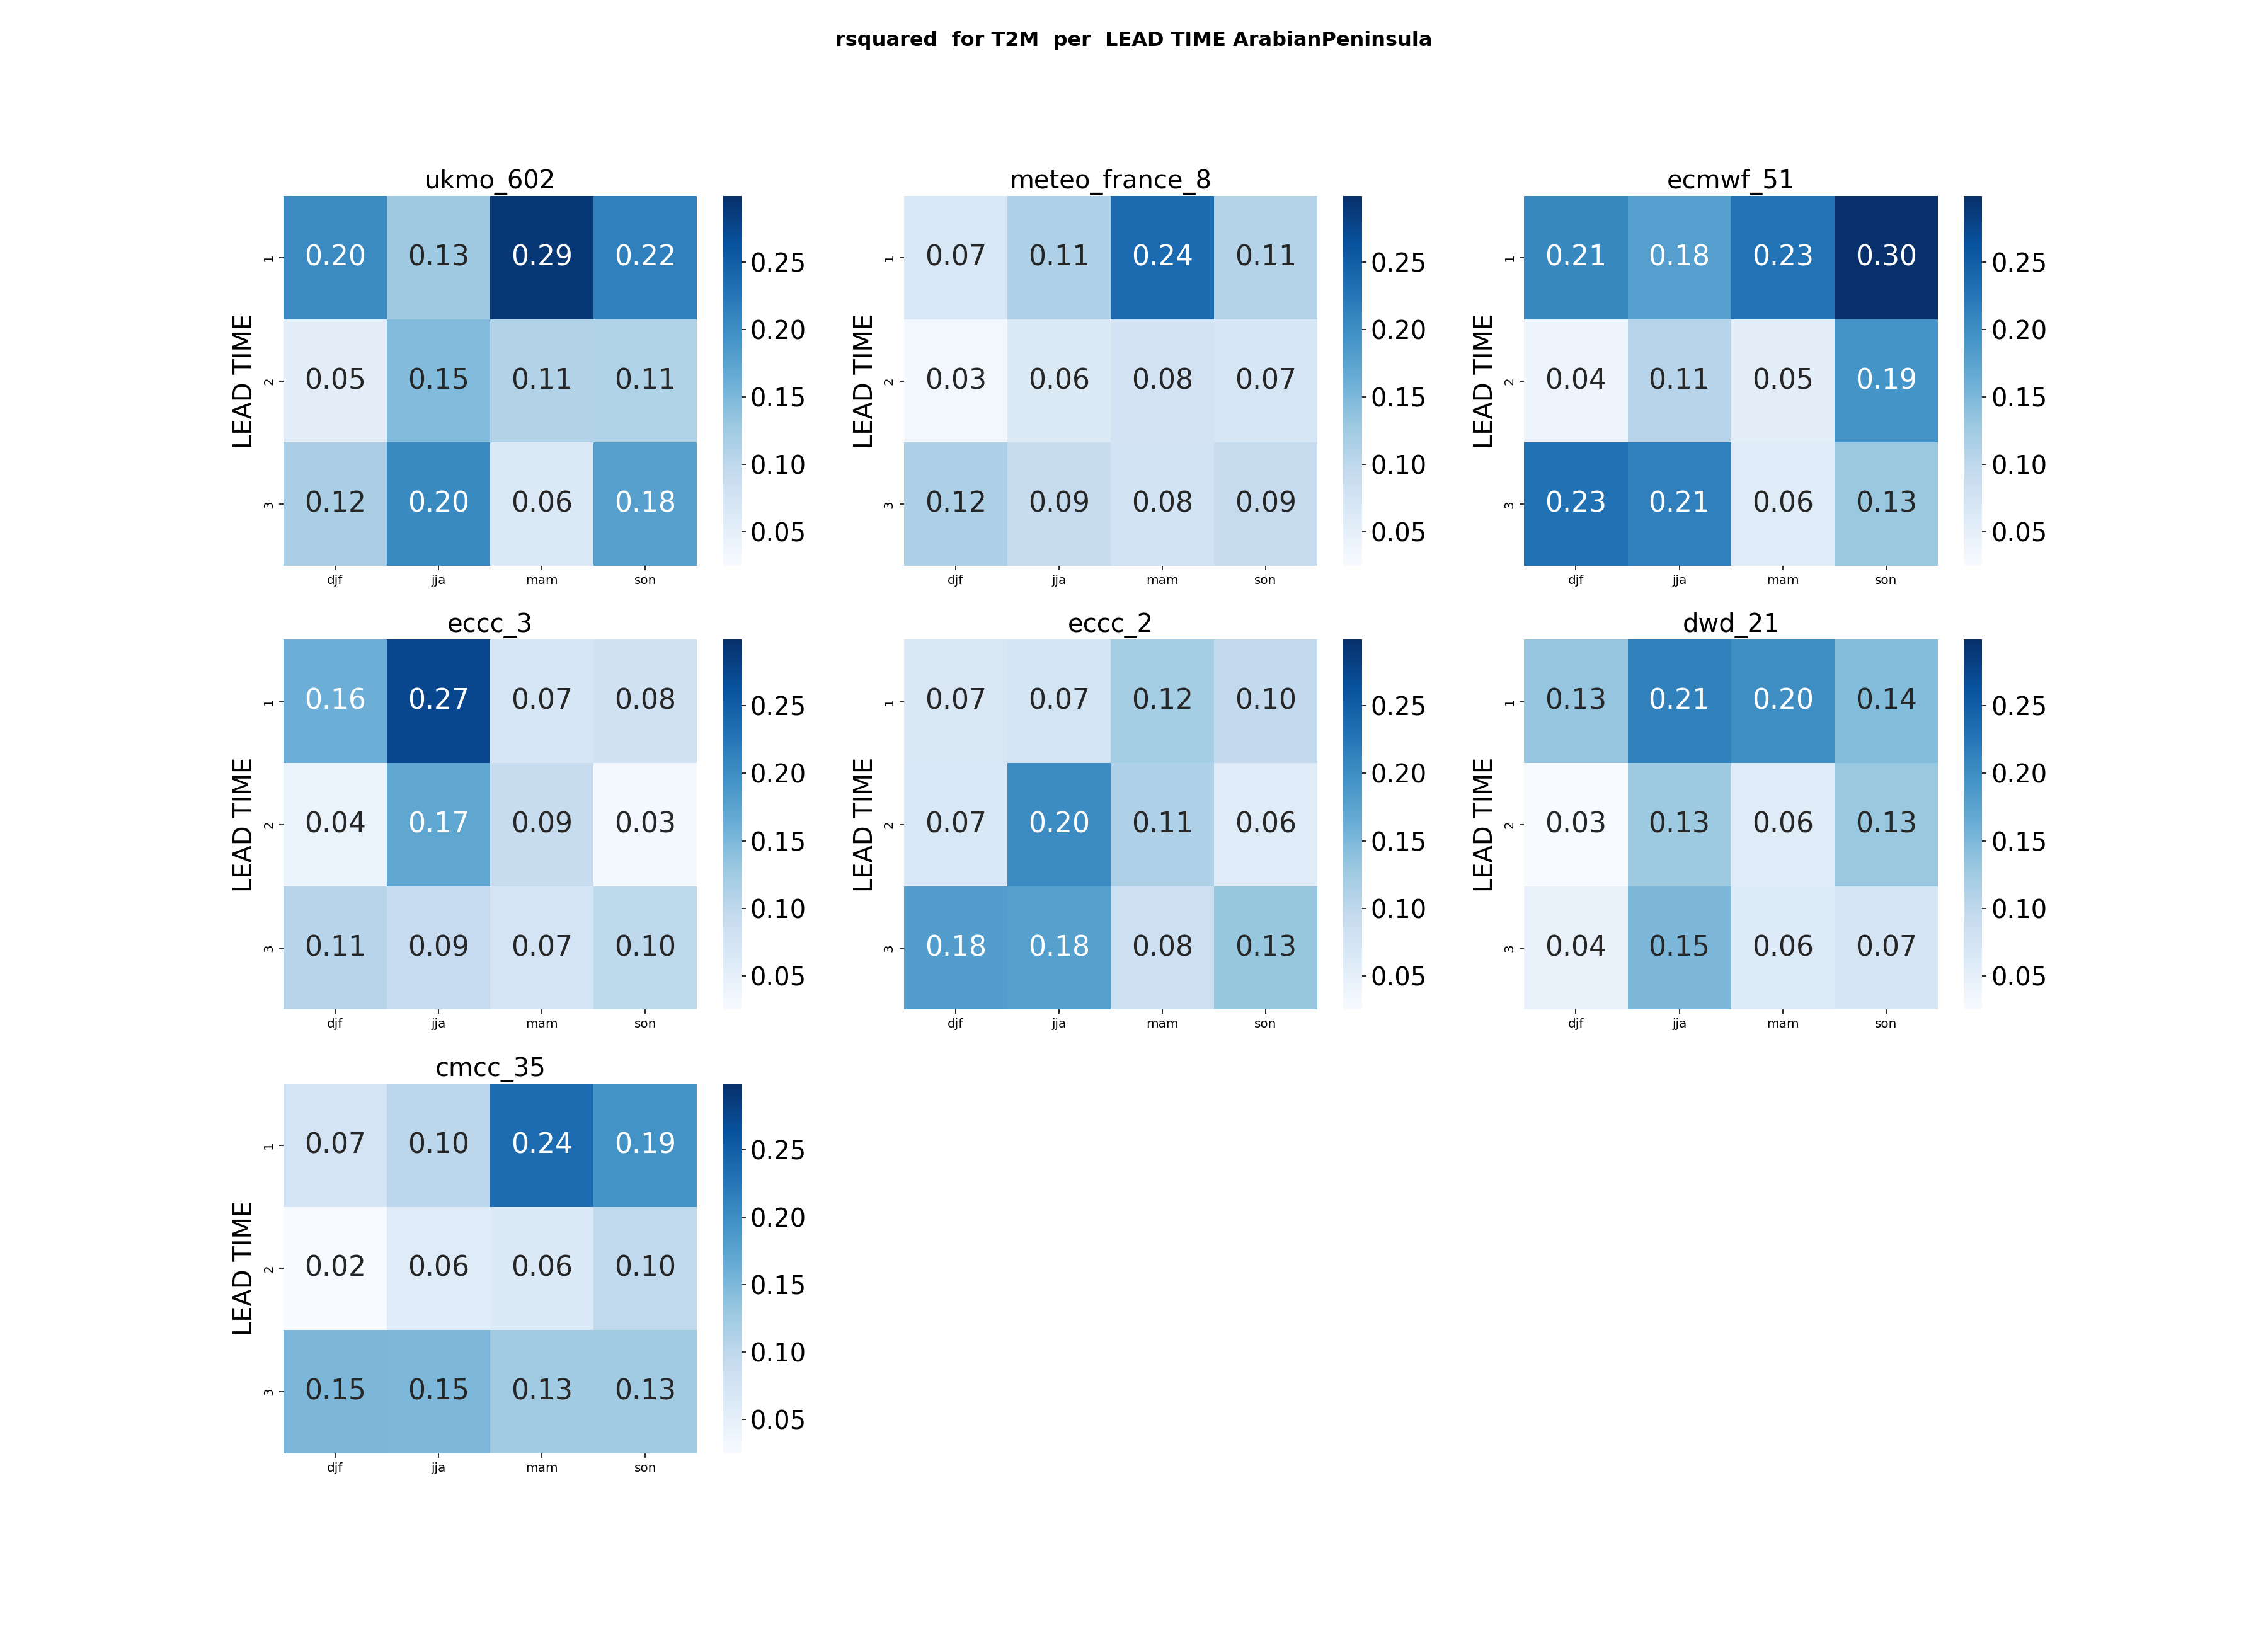
\includegraphics[scale=0.3]{plots/det/rsquared/rsquared_T2M_ArabianPeninsula.png}
\caption{Heatmap of T2M  RSQUARED in MENA Region for all centers Arabian Peninsula}
\end{figure}

the R-SQUARED for the Arabian Peninsula shows a little improvement.

\subsection{Probabilistic evaluation results}

To complement the deterministic evaluation of model performance, probabilistic evaluation metrics are employed to assess the reliability and skill of climate models in predicting the likelihood of specific outcomes. Unlike deterministic metrics, which focus on the accuracy of single-point predictions, probabilistic metrics evaluate the quality of the models’ forecast distributions, accounting for uncertainty and variability in predictions. These metrics are essential for understanding how well models represent the range of possible outcomes, particularly in regions like MENA, where climatic variability and extremes are prominent. By incorporating probabilistic metrics, this analysis provides a more comprehensive evaluation of the models’ predictive capabilities and their usefulness in decision-making under uncertainty.
The figures illustrate two main approaches to probabilistic assessment metrics, including the Brier Score (BS) and others. The first approach averages across lead times and grid points, while preserving categories, where the final figure contains the value of the metric for each season across all four seasons, for each category (mean, lower, upper) defined by the 1/3 quartiles. This method provides insight into the predictive ability of models under different seasonal conditions and forecast probability categories, particularly how well models capture temperature variations in the middle, lower, and upper quartiles of the predicted probability distribution. The diversity of metric values ​​across these categories helps highlight the sensitivity of models to different levels of forecast confidence. It indicates their ability to differentiate between forecast uncertainty and actual observed outcomes, providing a nuanced understanding of how accurately models predict different temperature ranges.

The second approach averages all grid points in the MENA region while retaining all lead times and seasons. This aggregated view provides an overall assessment of the measure for each season, considering all lead times and forecast categories. This approach focuses on how models perform across different forecast scenarios and how well they produce accurate and reliable temperature forecasts, regardless of forecast probability. By retaining lead times and seasons in the analysis, this method provides a comprehensive picture of model performance over time and under different climate conditions. It reveals how well models generalize across different forecast scenarios, helping to identify which models are most effective at producing consistent and reliable forecasts.
\subsubsection{Brier score}

The figure at the bottom illustrates that most models demonstrate relatively high performance, as indicated by a small Brier Score (BS) around 0.2, meaning that the predicted probabilities are close to the observed ones. This reflects accurate forecast probabilities for T2M. Notably, the middle category presents lower performance relative to the other two categories (lower and upper). This indicates that while some models capture temperature variability well in extreme conditions (upper category), their skill may diminishes when forecasting moderate changes (middle category). This discrepancy highlights the challenges models face in translating predicted probabilities into reliable forecasts, particularly for temperature variations that are neither extreme nor outlier events. 


\begin{figure}[H]
    \centering
    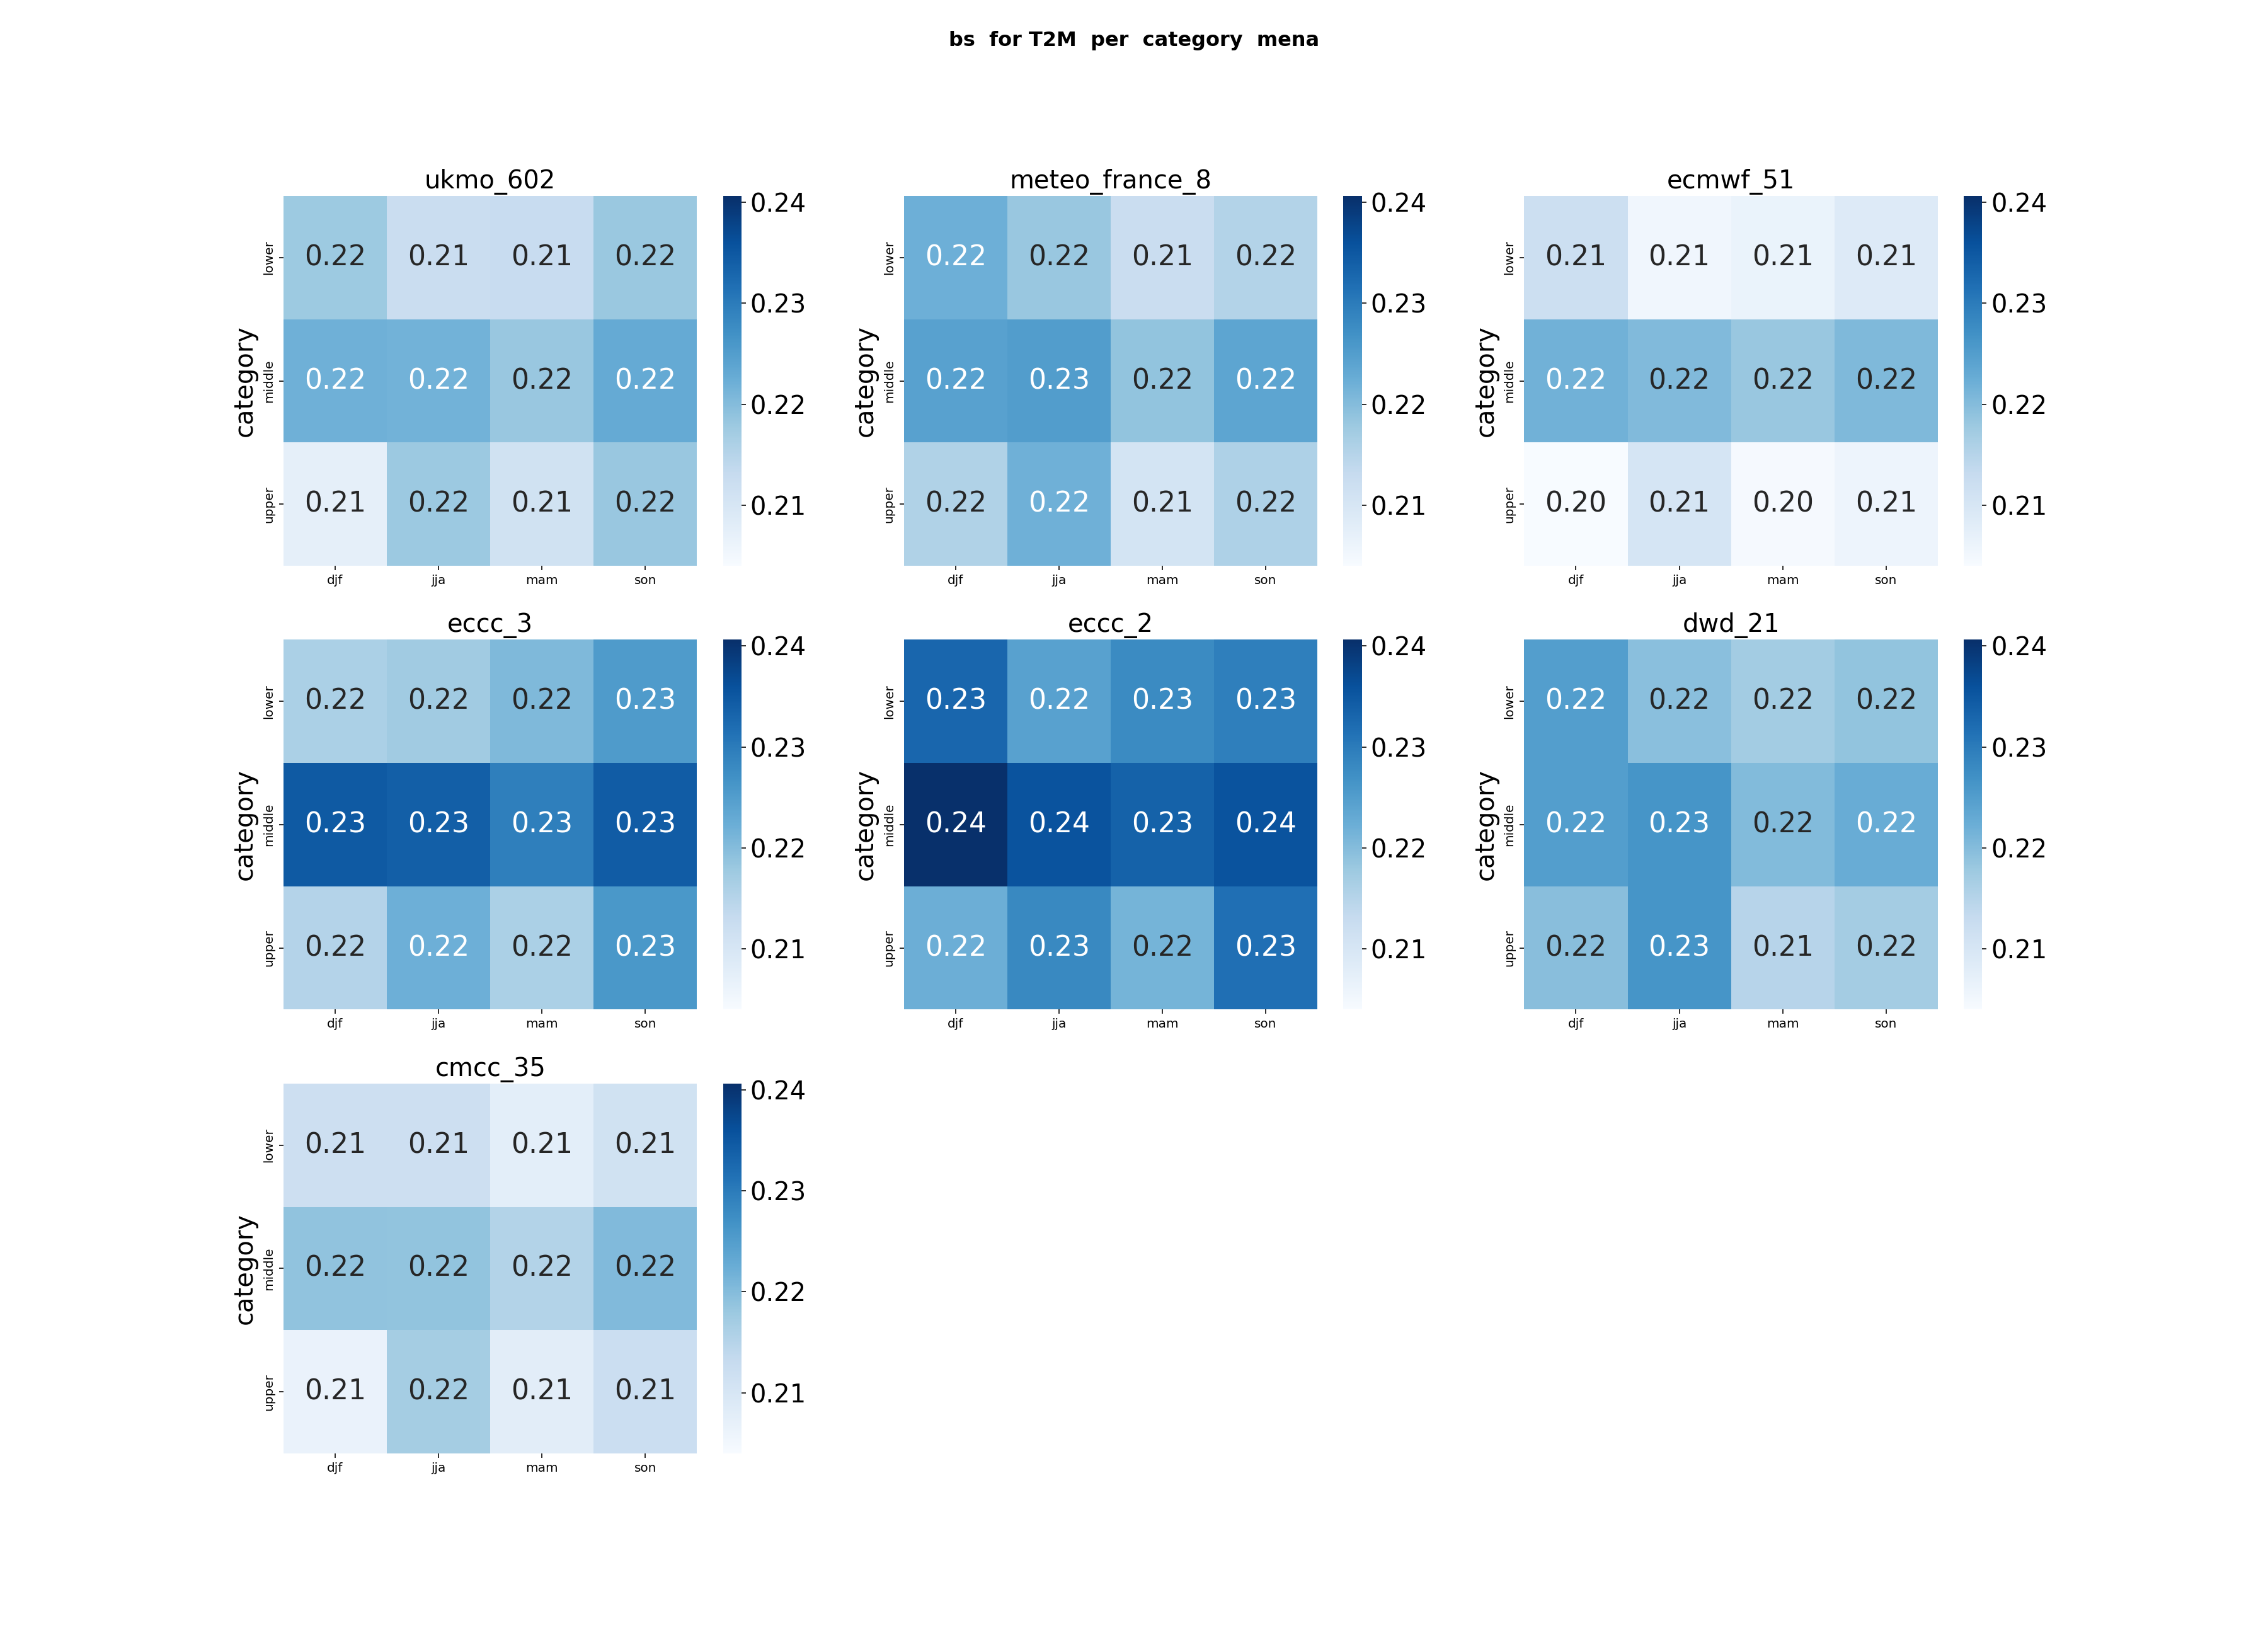
\includegraphics[width=1\linewidth]{plots/prob/bs/bs_T2M_category_mena.png}
    \caption{Temperature Brier score heatmaps for all the seasons per categories \textbf{\textit{(0 represents perfect BS)} }}
\end{figure}

An analysis by lead time revealed that the models \textbf{\textit{ Meteo France, ECMWF,UKMO  and CMCC-35 }} exhibit superior performance, as indicated by lower Brier Scores (BS) between 0.21 and 0.23. This suggests that these models provide more accurate probabilistic forecasts for T2M compared to others. Moreover, the differences in BS values between successive lead times are minimal, indicating that the predictive skill of these models remains relatively consistent as the forecast horizon increases.

This stability in performance across lead times is particularly noteworthy, as it reflects the robustness of these models in maintaining their ability to produce reliable forecasts over time. The lower BS values also suggest that these models effectively capture the relationship between predicted probabilities and observed outcomes, ensuring high confidence in their probabilistic predictions. Such consistent performance across lead times is crucial for operational forecasting, as it highlights these models' reliability for both short- and medium-term forecasts in the MENA region.

\begin{figure}[H]
    \centering
    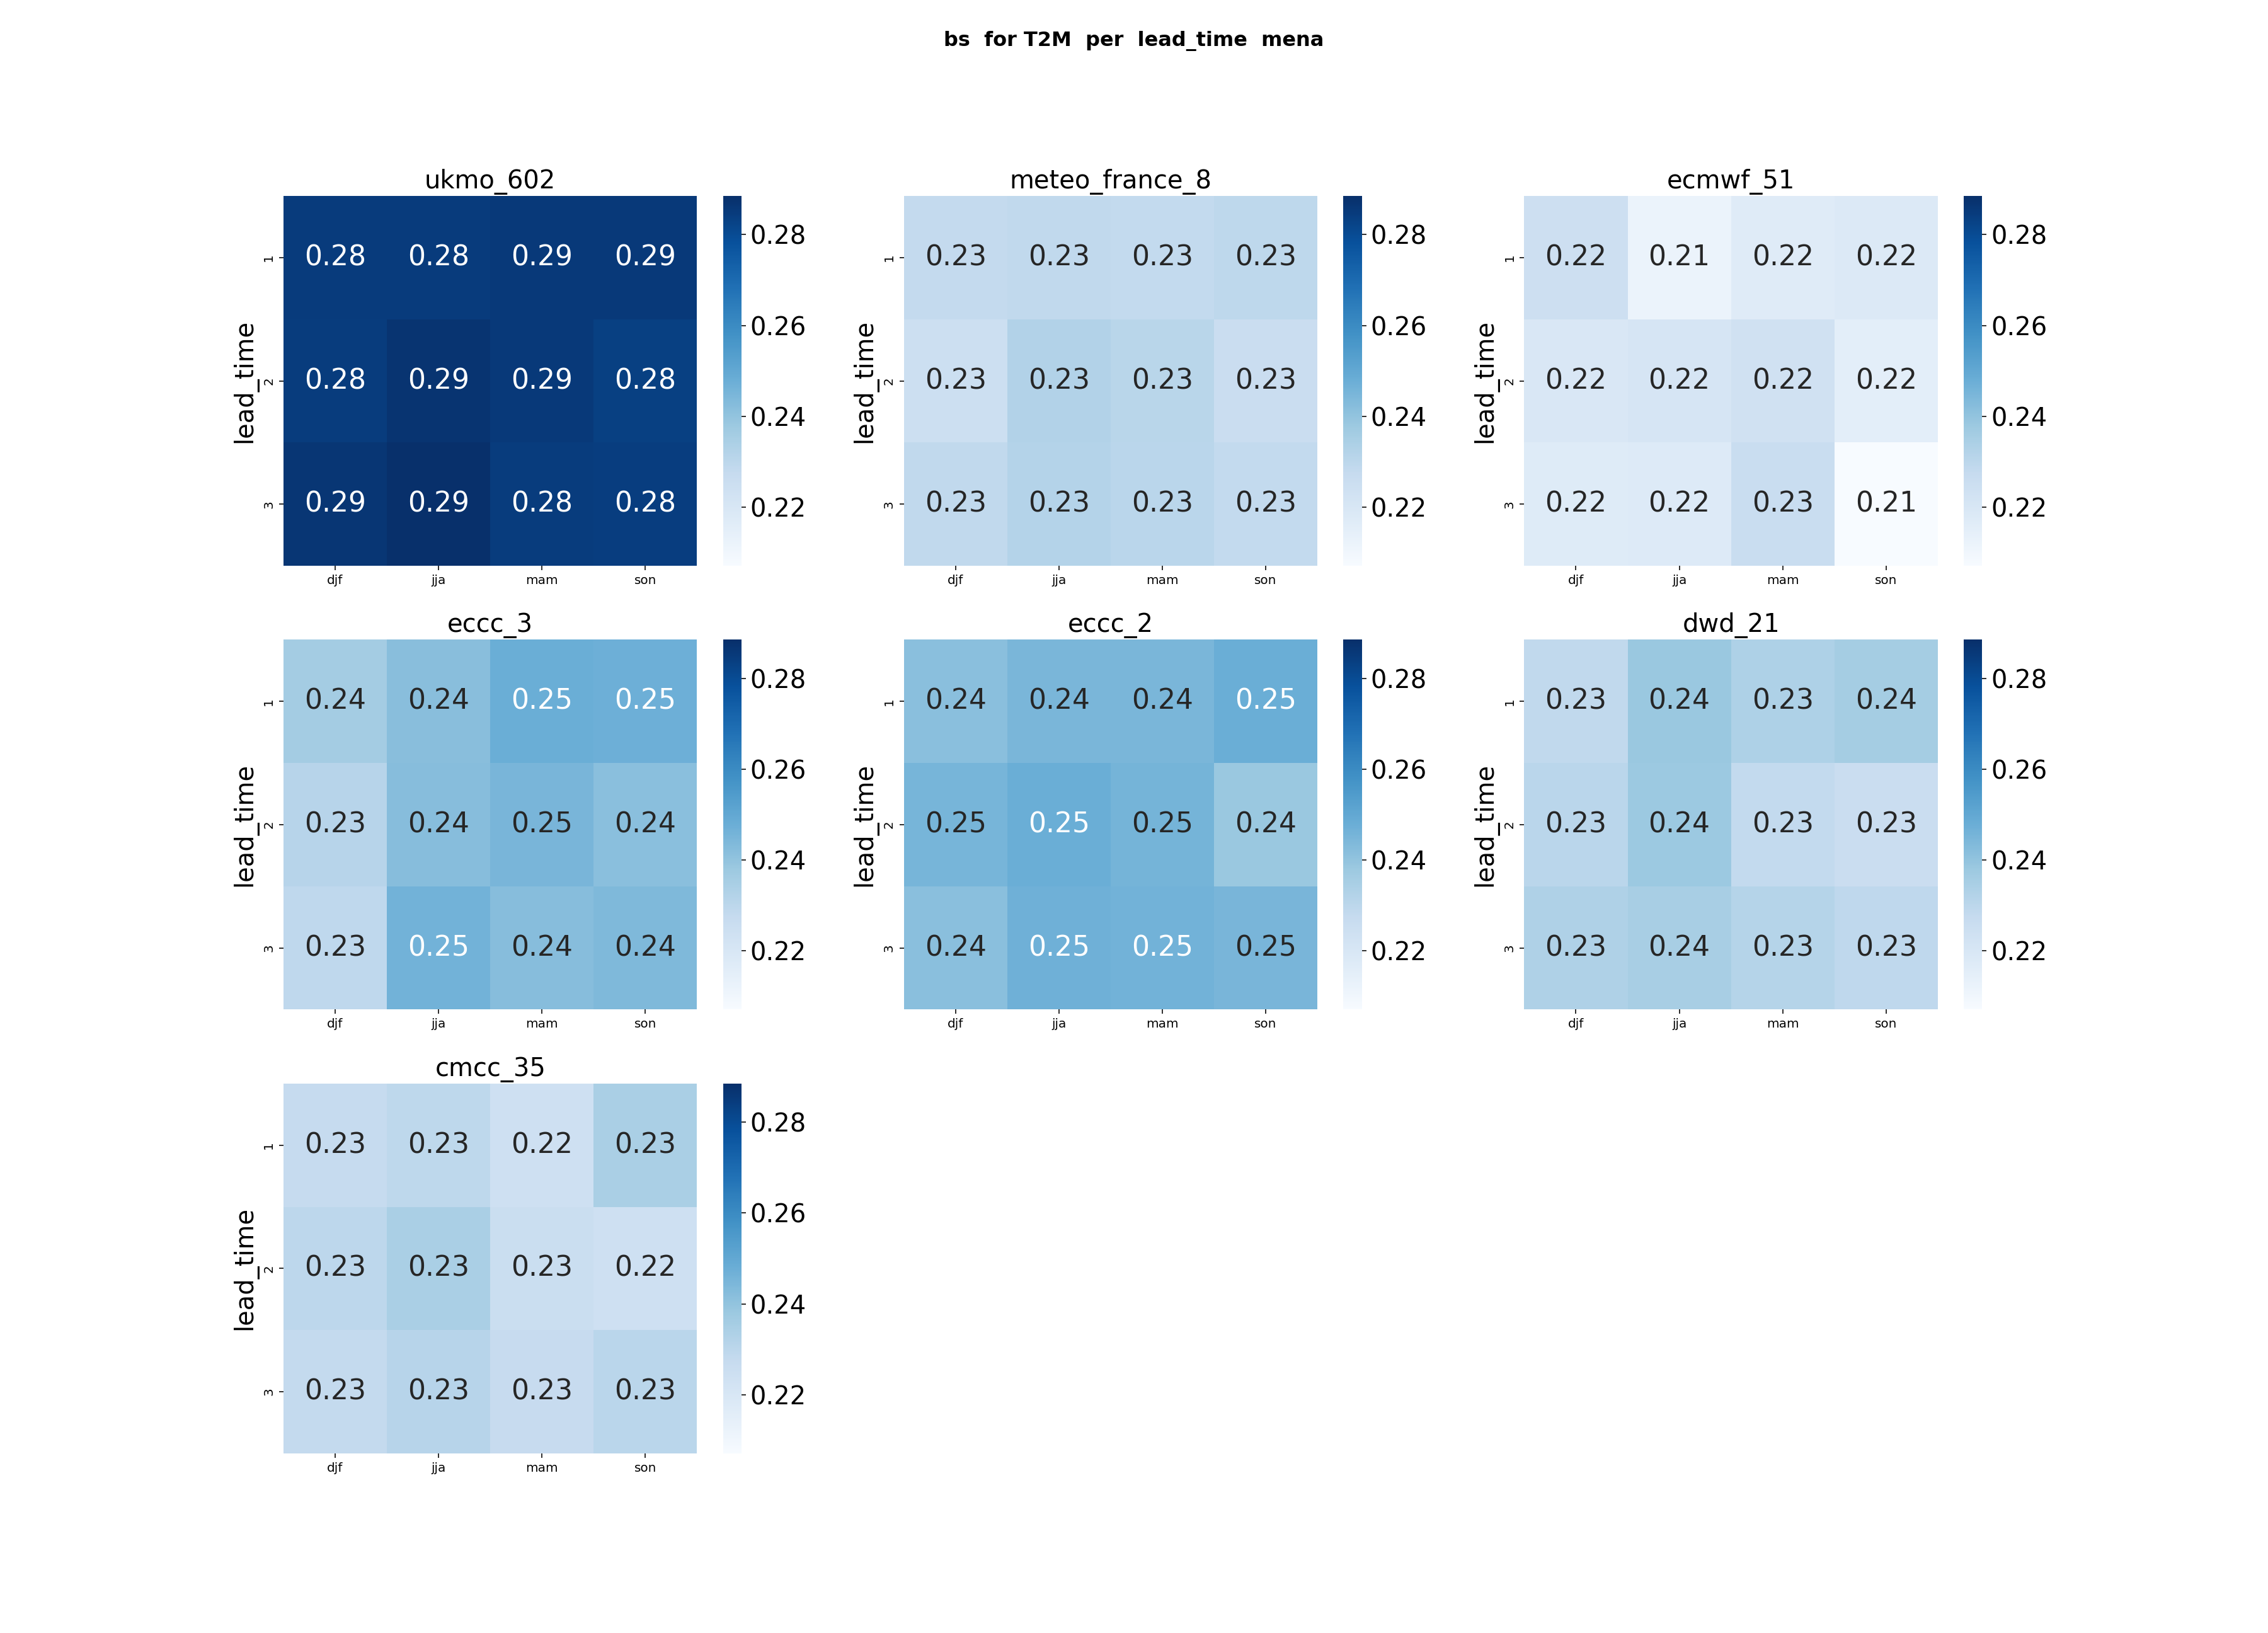
\includegraphics[width=1\linewidth]{plots/prob/bs/bs_T2M_lead_time_mena.png}
    \caption{Temperature brier score heatmaps for all the seasons per lead time \textbf{\textit{(0 represents perfect BS)} }}
\end{figure}


\begin{figure}[H]
    \centering
    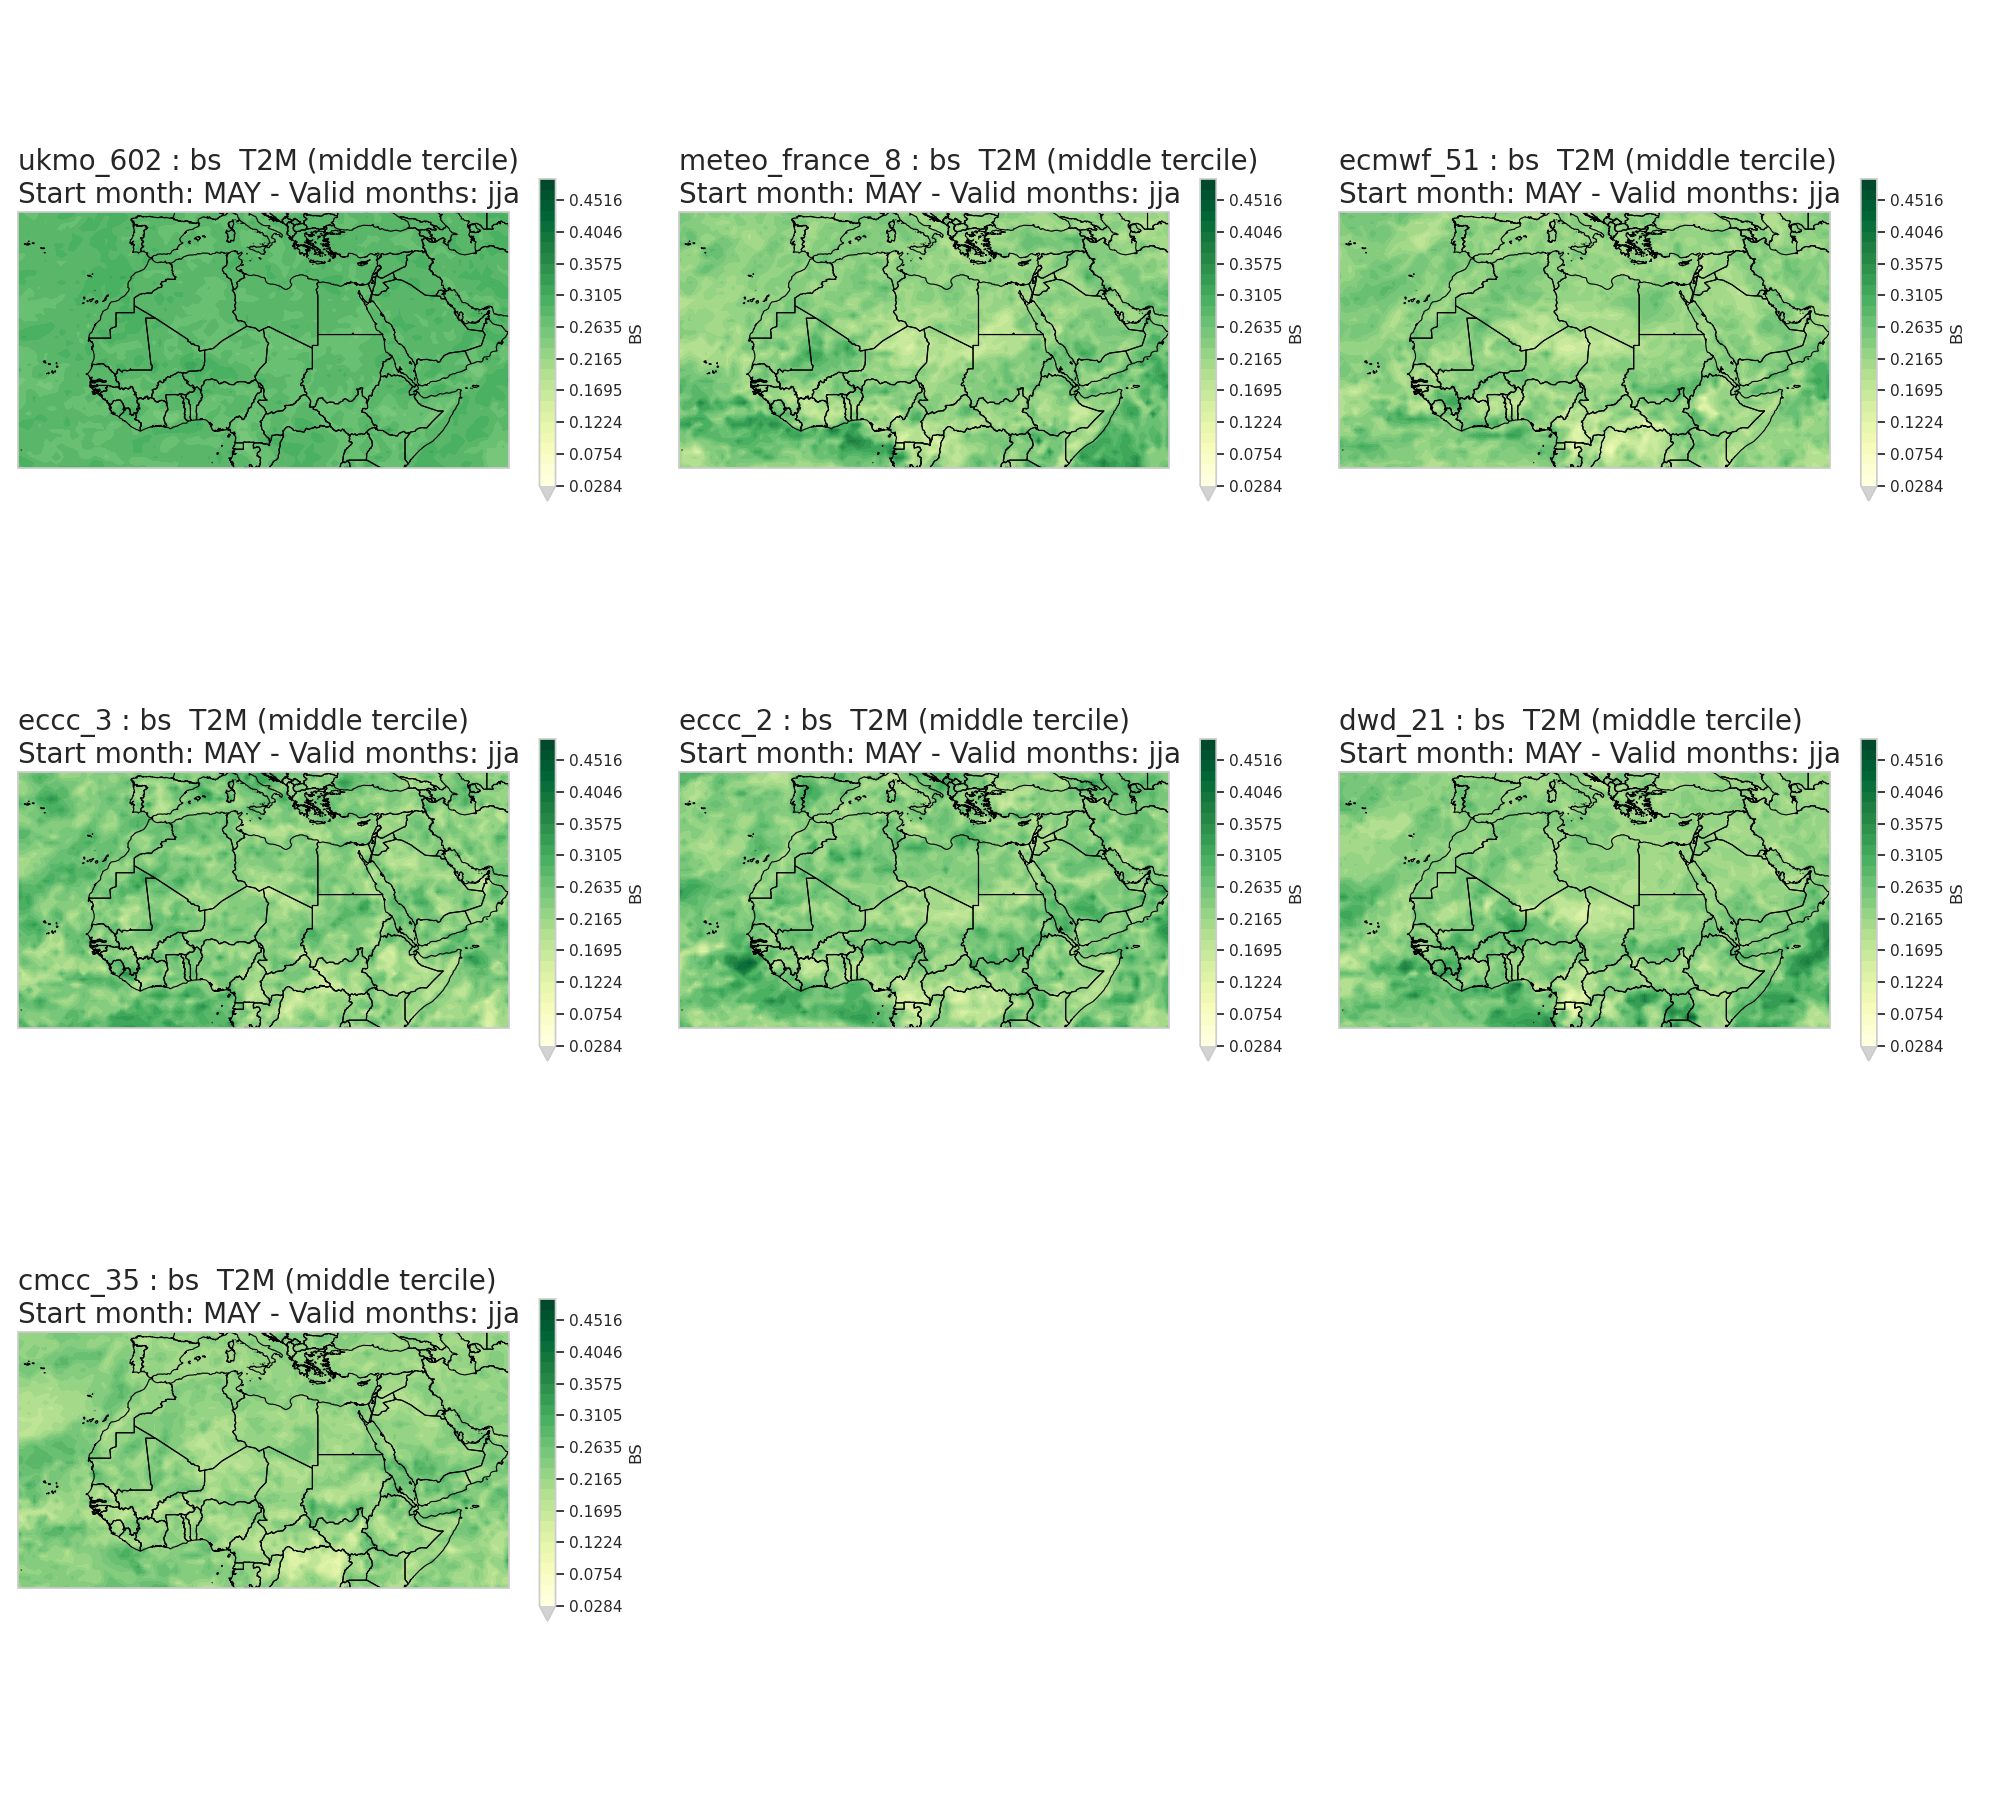
\includegraphics[width=1\linewidth]{plots/prob/bs/bs_jja_t2m_middle.png}
    \caption{3 months rolling mean for 2-meter-temperature of brier score in the middle tercile JJA. \textbf{\textit{(0 represents perfect BS)} }}
\end{figure}

For the \textbf{\textit{ECMWF}}, the Brier Score reaches an impressive value of 0.02 at the equator, signifying an exceptionally high level of forecast reliability and accuracy in this region. This score underscores the center's strong capability to generate precise probabilistic forecasts, particularly in equatorial zones where weather patterns can be highly dynamic.

While the other centers exhibit a slight decrease in performance compared to the \textbf{\textit{ECMWF}}, their results still fall within the range of noteworthy accuracy. The relatively modest decline does not overshadow the overall competency demonstrated by the centers, as their scores remain indicative of robust forecasting.

This comprehensive evaluation of Brier Scores across different centers reflects an impressive level of \textbf{Resolution}, which refers to the ability of a forecast to distinguish between different outcomes effectively. 

\paragraph{focus on North Africa}:

To evaluate model performance in North Africa, Brier Score analysis confirms that \textbf{\textit{ECMWF, CMCC, and UKMO}} maintain low scores, reflecting consistent reliability across lead times and seasons. These findings indicate that North Africa’s unique climatic variability does not significantly impact the predictive skill of these models, affirming their adaptability within the broader MENA region. Minimal score variations across lead times further emphasize their robustness for accurate probabilistic forecasting over varying temporal ranges.

\begin{figure}[H]
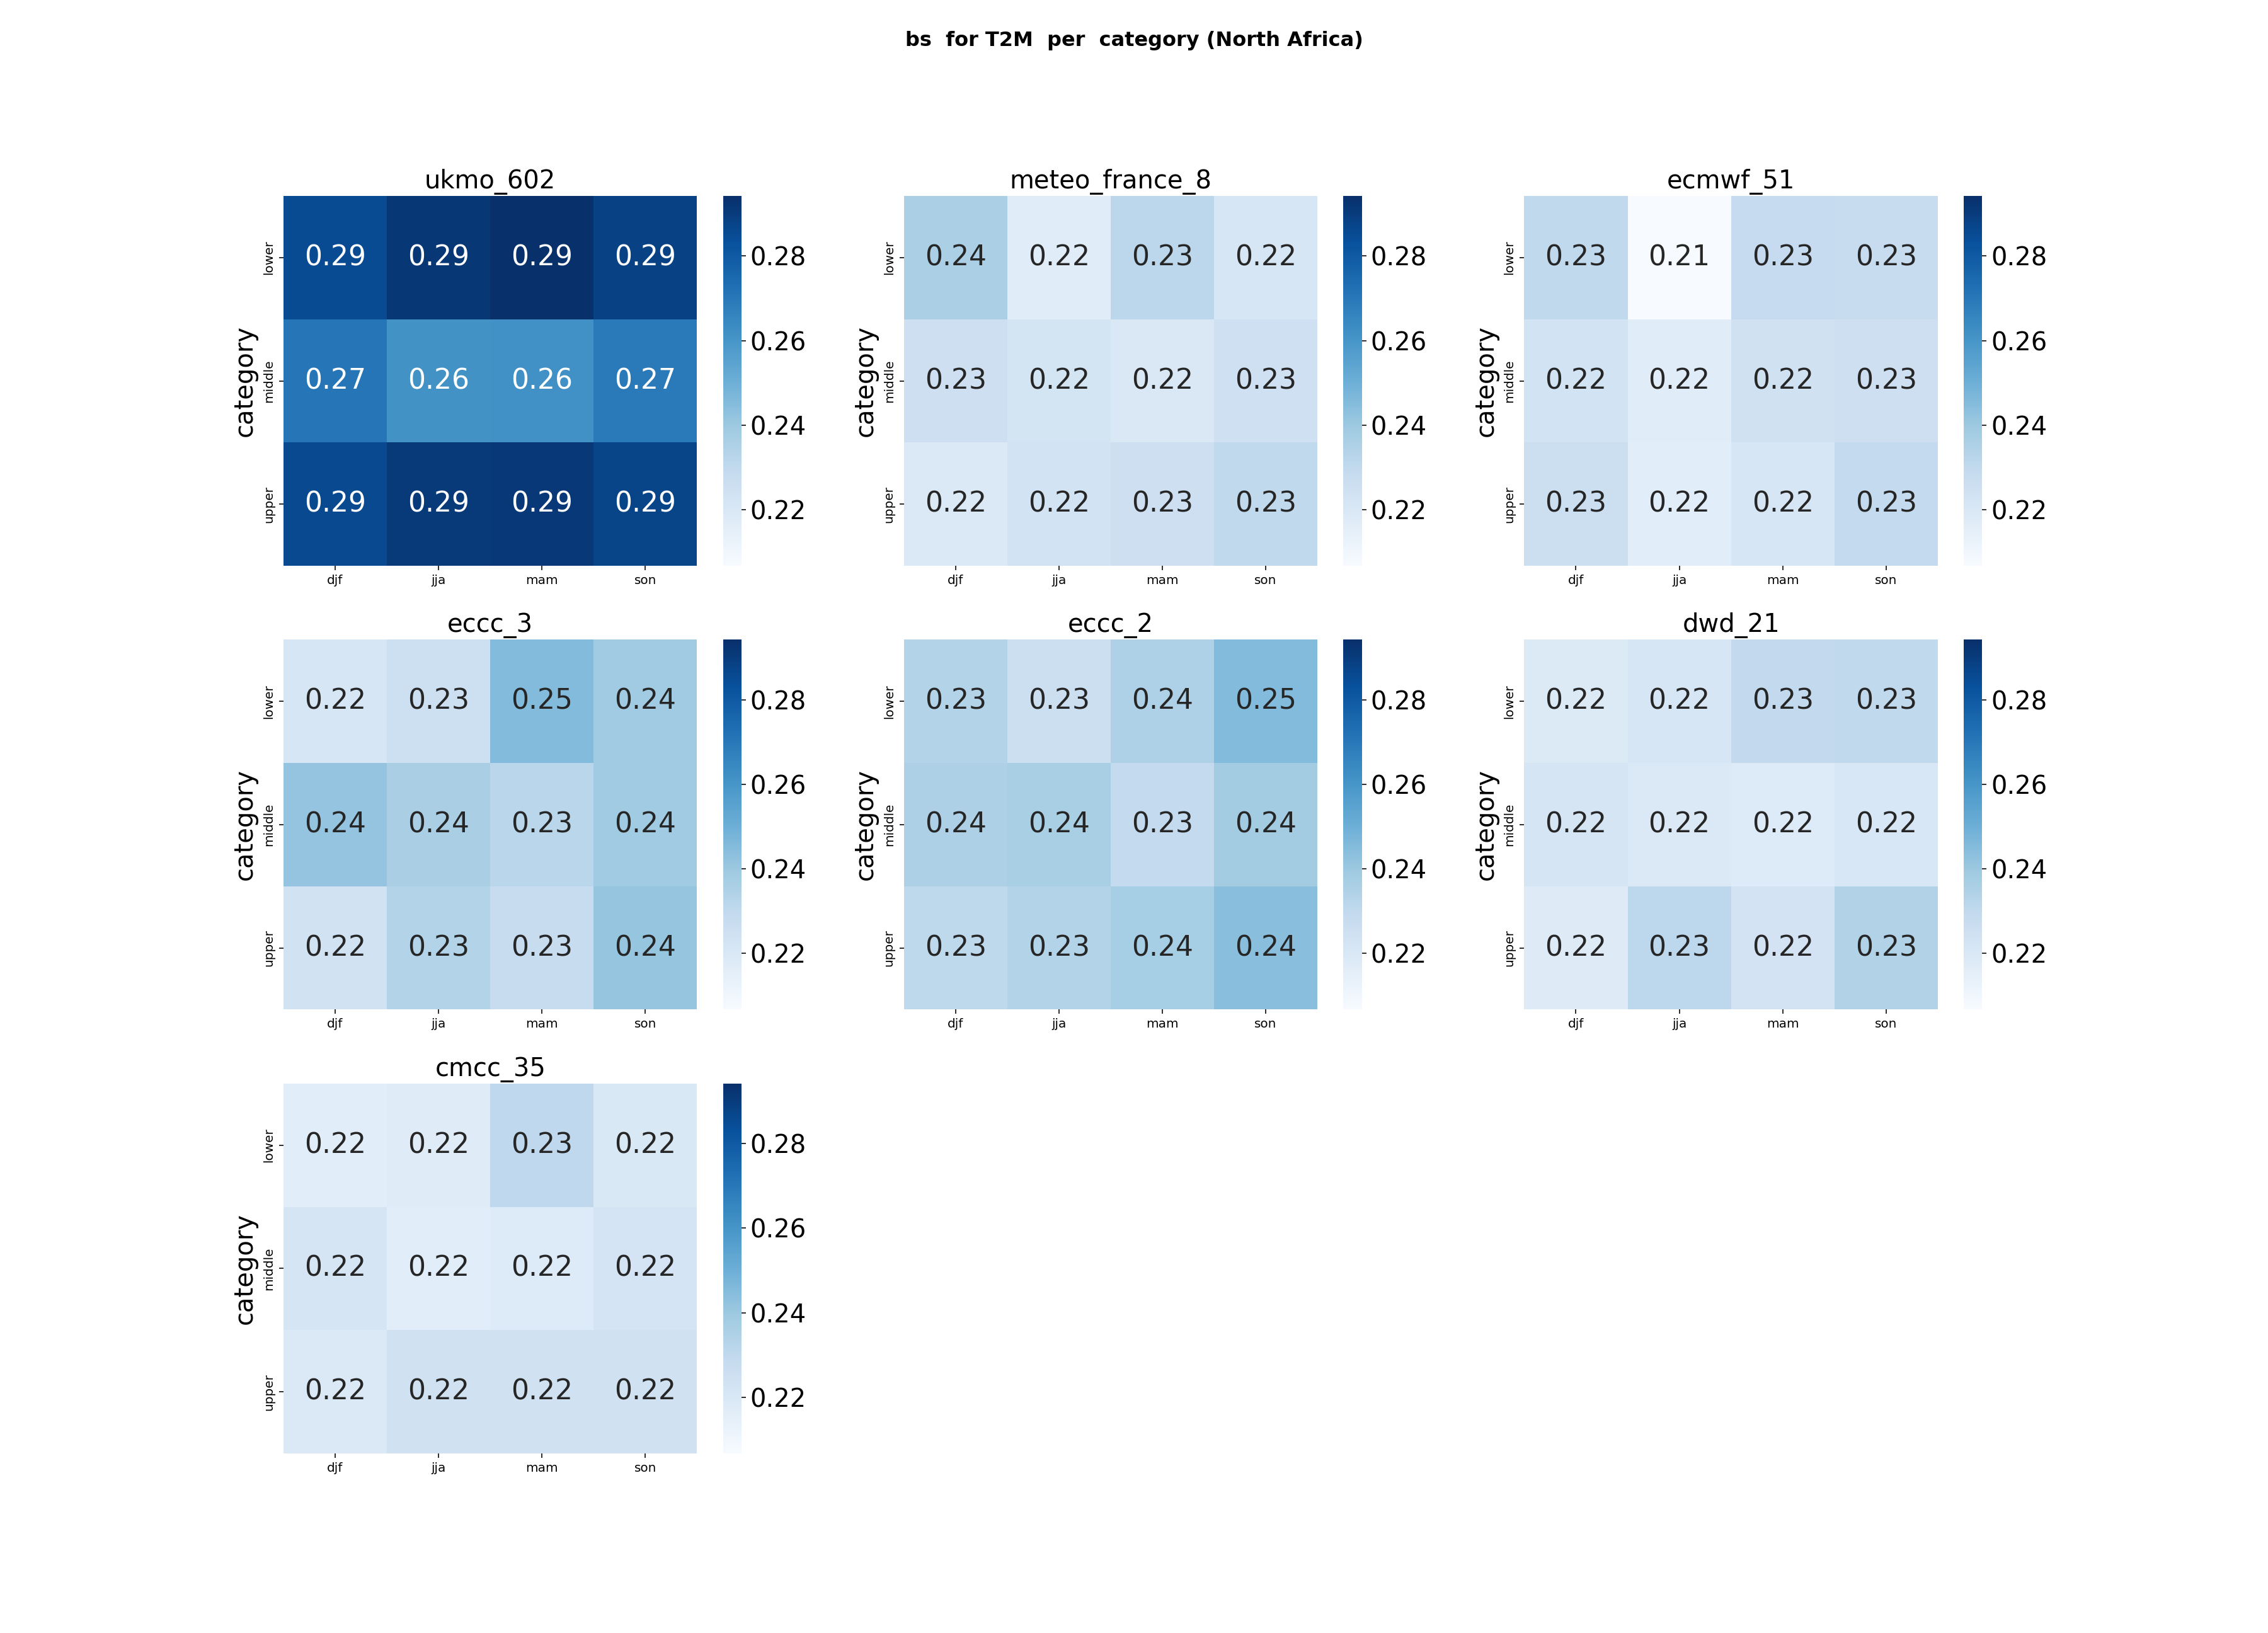
\includegraphics[scale=0.3]{plots/prob/bs/bs_T2M_category_NorthAfrica.png}

\caption{Heatmap of T2M  brier score for all centers in North Africa region}
\end{figure}





\vspace{1.5cm}
\paragraph{focus on Arabian Peninsula}:
there is no big difference in Arabian Peninsula.

\subsubsection{Reliability}

\begin{figure}[H]
    \centering
    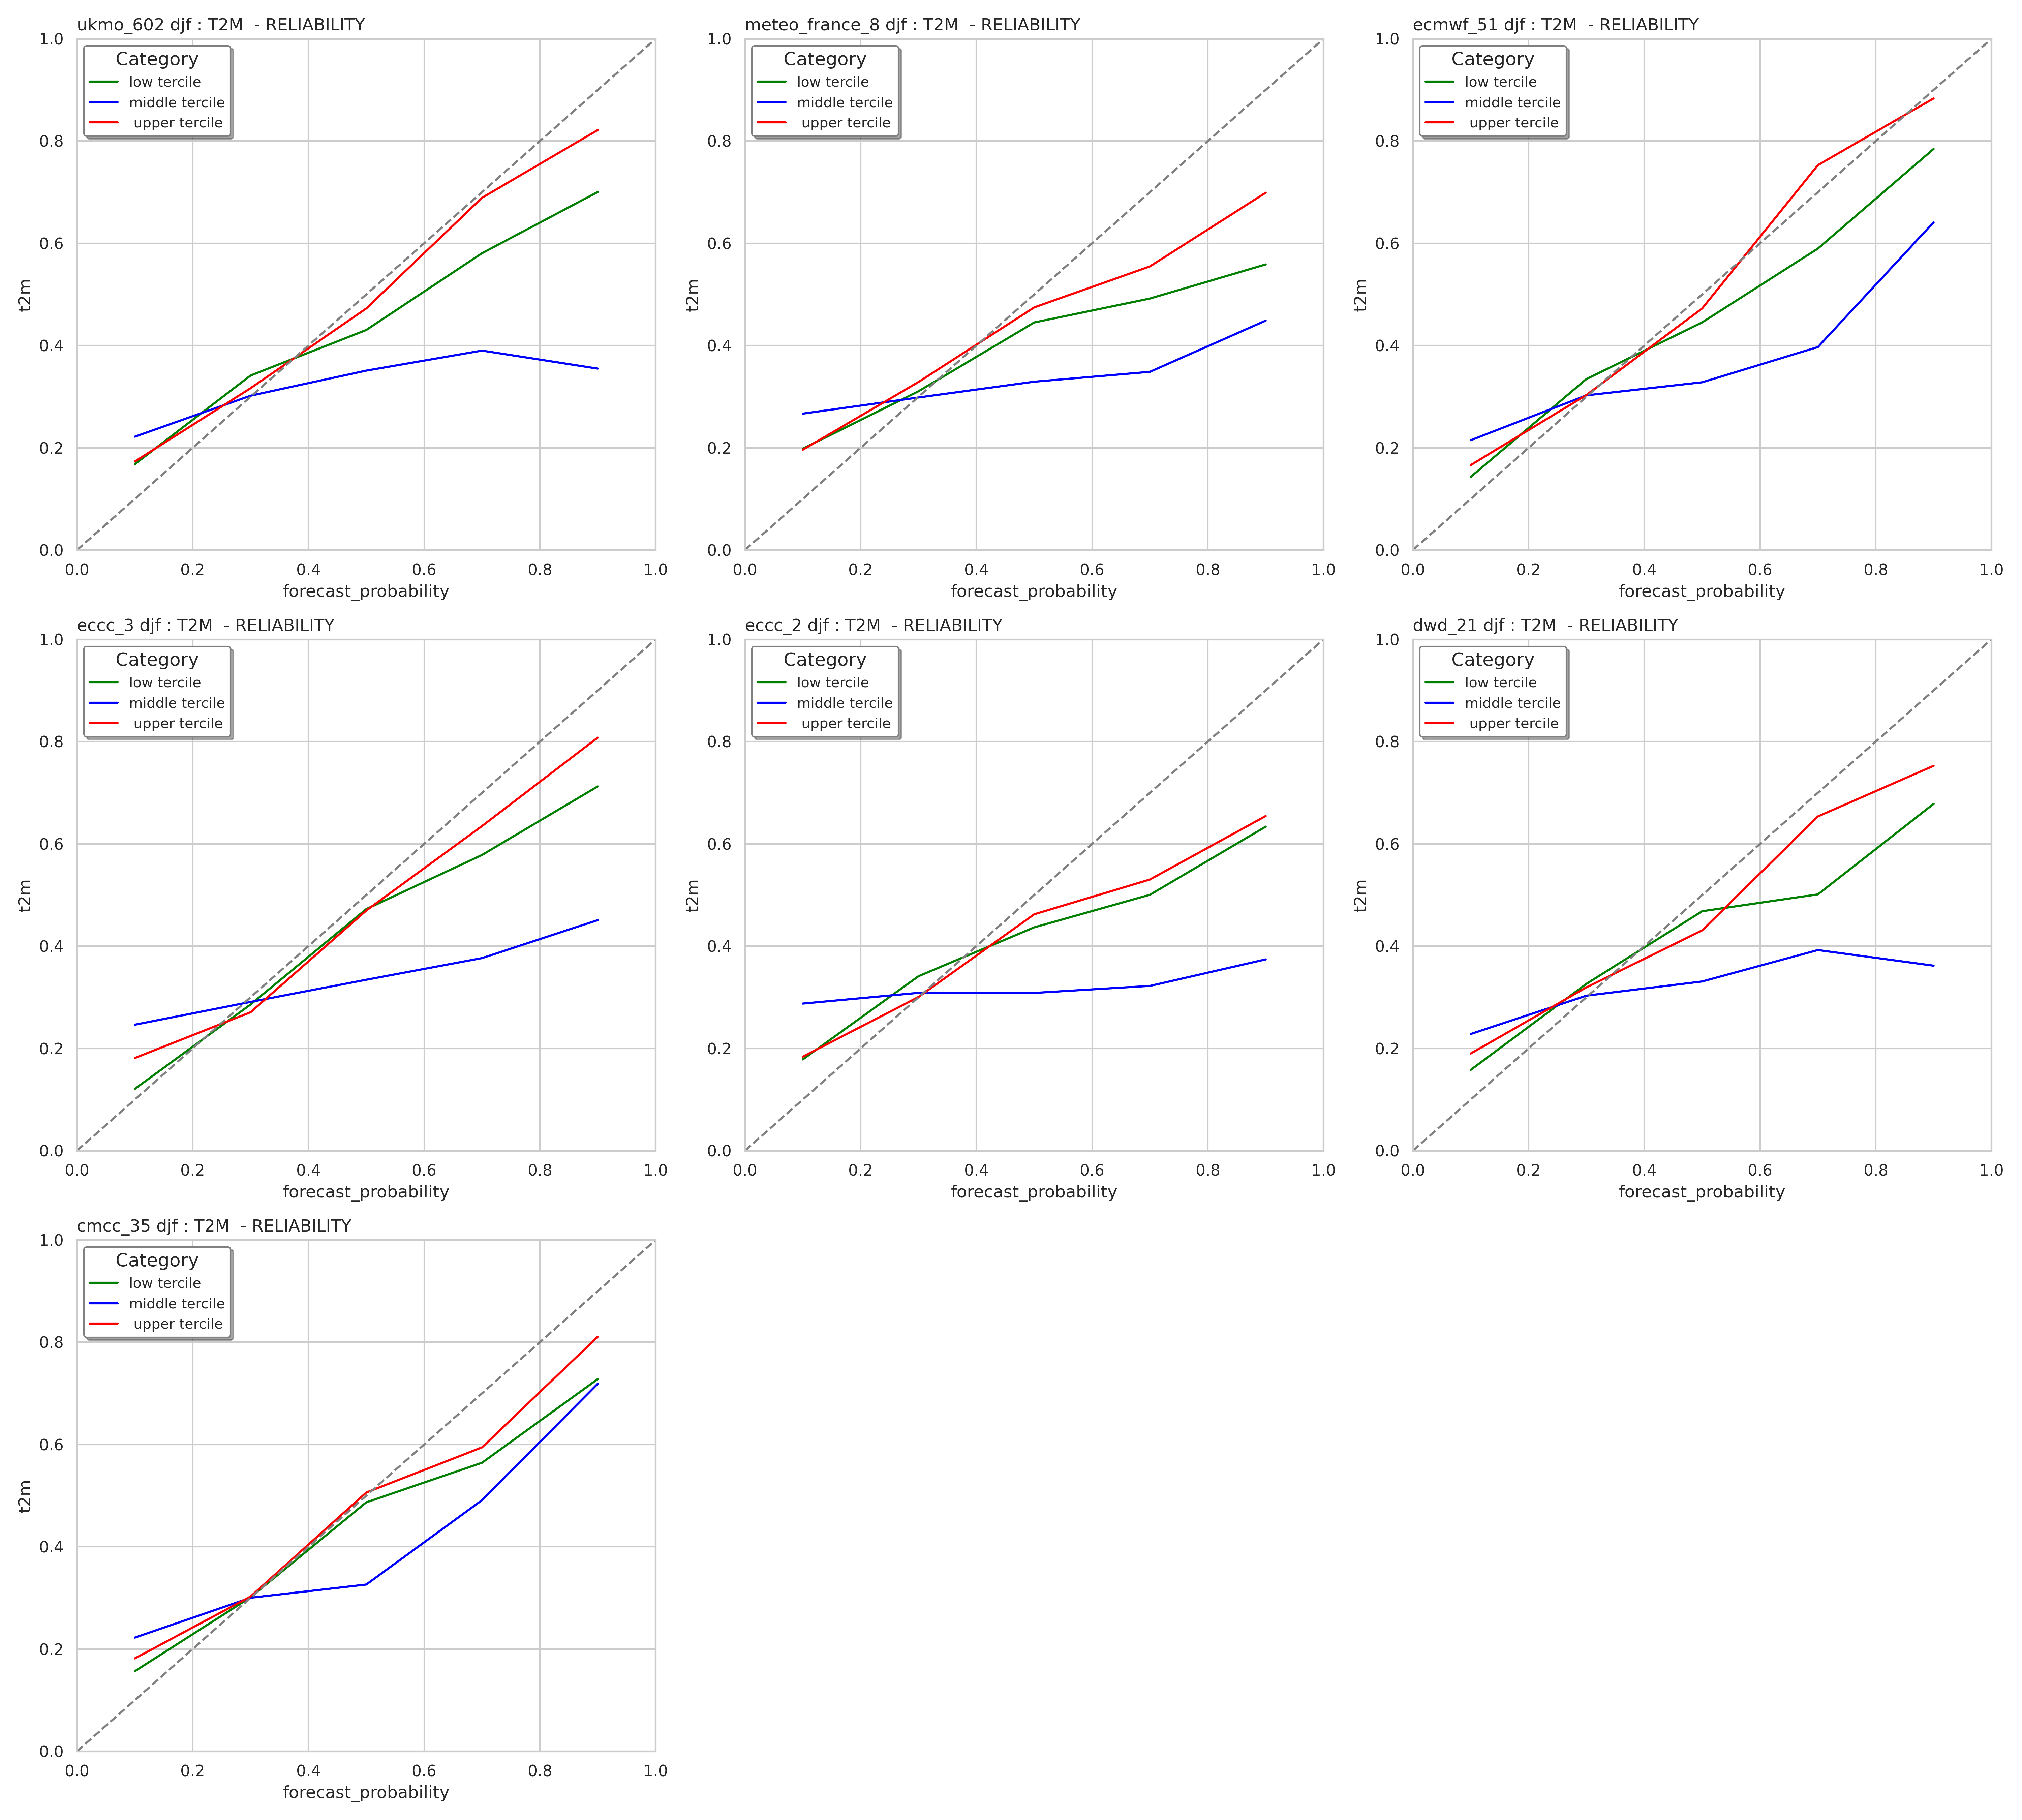
\includegraphics[width=1\linewidth]{plots/prob/rela/rela_diagram_djf_t2m.png}
    \caption{temperature reliability diagram DJF \textbf{\textit{(45 degree means perfect reliability)}}}
\end{figure}

The reliability diagram reveals strong performance in predicting the upper and lower terciles across all centers, with particularly notable accuracy observed in \textbf{\textit{UKMO, ECMWF, and ECCC-3}}. However, the middle tercile presents some notable challenges, with predictions being less reliable for all centers. Among them, the \textbf{\textit{CMCC-35}} demonstrates comparatively better performance in this middle range, indicating potential advantages in handling predictions for moderate conditions.

\begin{figure}[H]
    \centering
    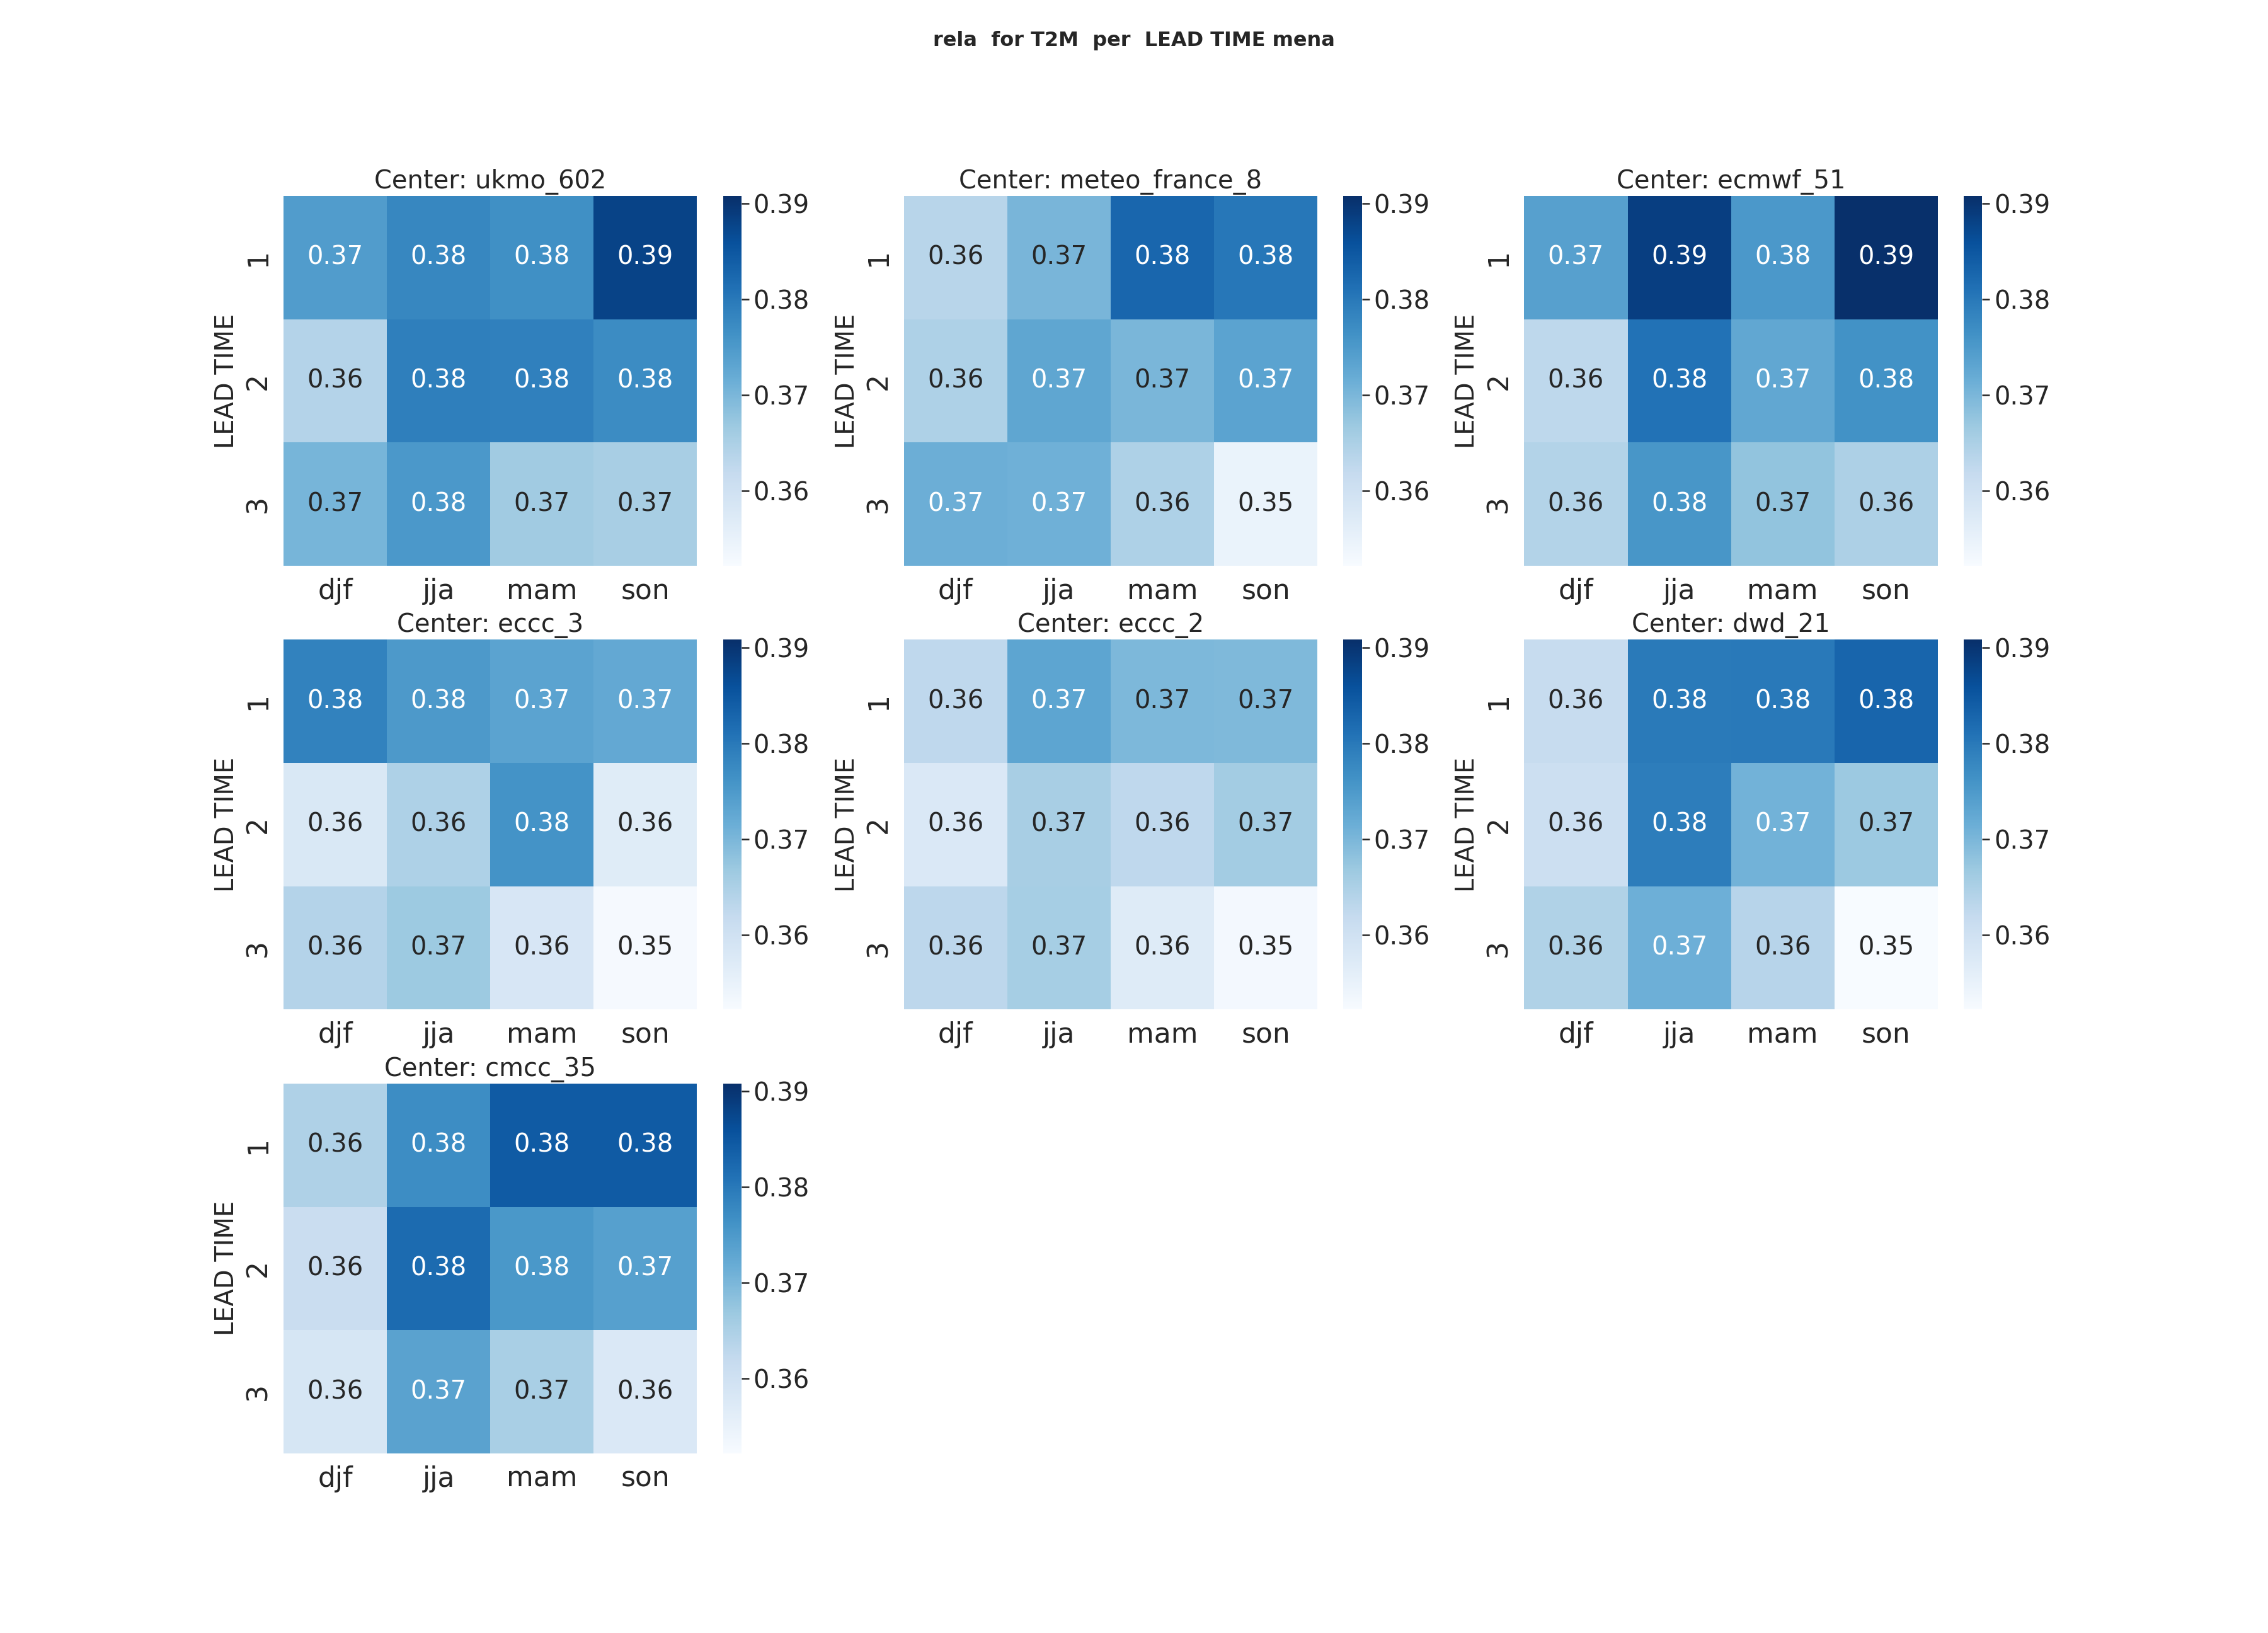
\includegraphics[width=1\linewidth]{plots/prob/rela/rela_T2M_mena.png}
    \caption{temperature reliability heatmap \textbf{\textit{(0 means perfect Reliability)}}}
\end{figure}


The heatmap highlights similar trends observed across the models and seasons. Thus, there is no big difference between centers, the score is moderate and the variability along lead-time is very week.


\paragraph{focus on North Africa}:
\begin{figure}[H]
\includegraphics[scale=0.3]{plots/prob/rela/rela_T2M_NorthAfrica.png}

\caption{Heatmap of T2M  reliability  for all centers in North Africa}
\end{figure}


A more focused analysis on North Africa has not significantly altered the overall conclusions derived from the broader MENA region. The consistent performance patterns observed across the different models and seasons remain largely unchanged when examining the North African context. 

\paragraph{focus on Arabian Peninsula}:

there is no big difference in  Arabian Peninsula.

\subsubsection{The ranked probability score}

The Ranked Probability Score (RPS) provides a valuable measure of forecast performance by evaluating the accuracy of probabilistic predictions across different categories. It combines both the skill in predicting the occurrence of events and the sharpness of the forecast distribution. By comparing the forecasted probability distribution against the observed outcomes, the RPS quantifies the deviation between the predicted and actual probabilities. A lower RPS value indicates better forecast accuracy, reflecting both how well the forecast aligns with observed frequencies and how well it discriminates between different probability categories. This metric helps to identify which models offer the most reliable probabilistic predictions, particularly in terms of capturing the likelihood of various temperature outcomes within a given forecast period.
\begin{figure}[H]
    \centering
    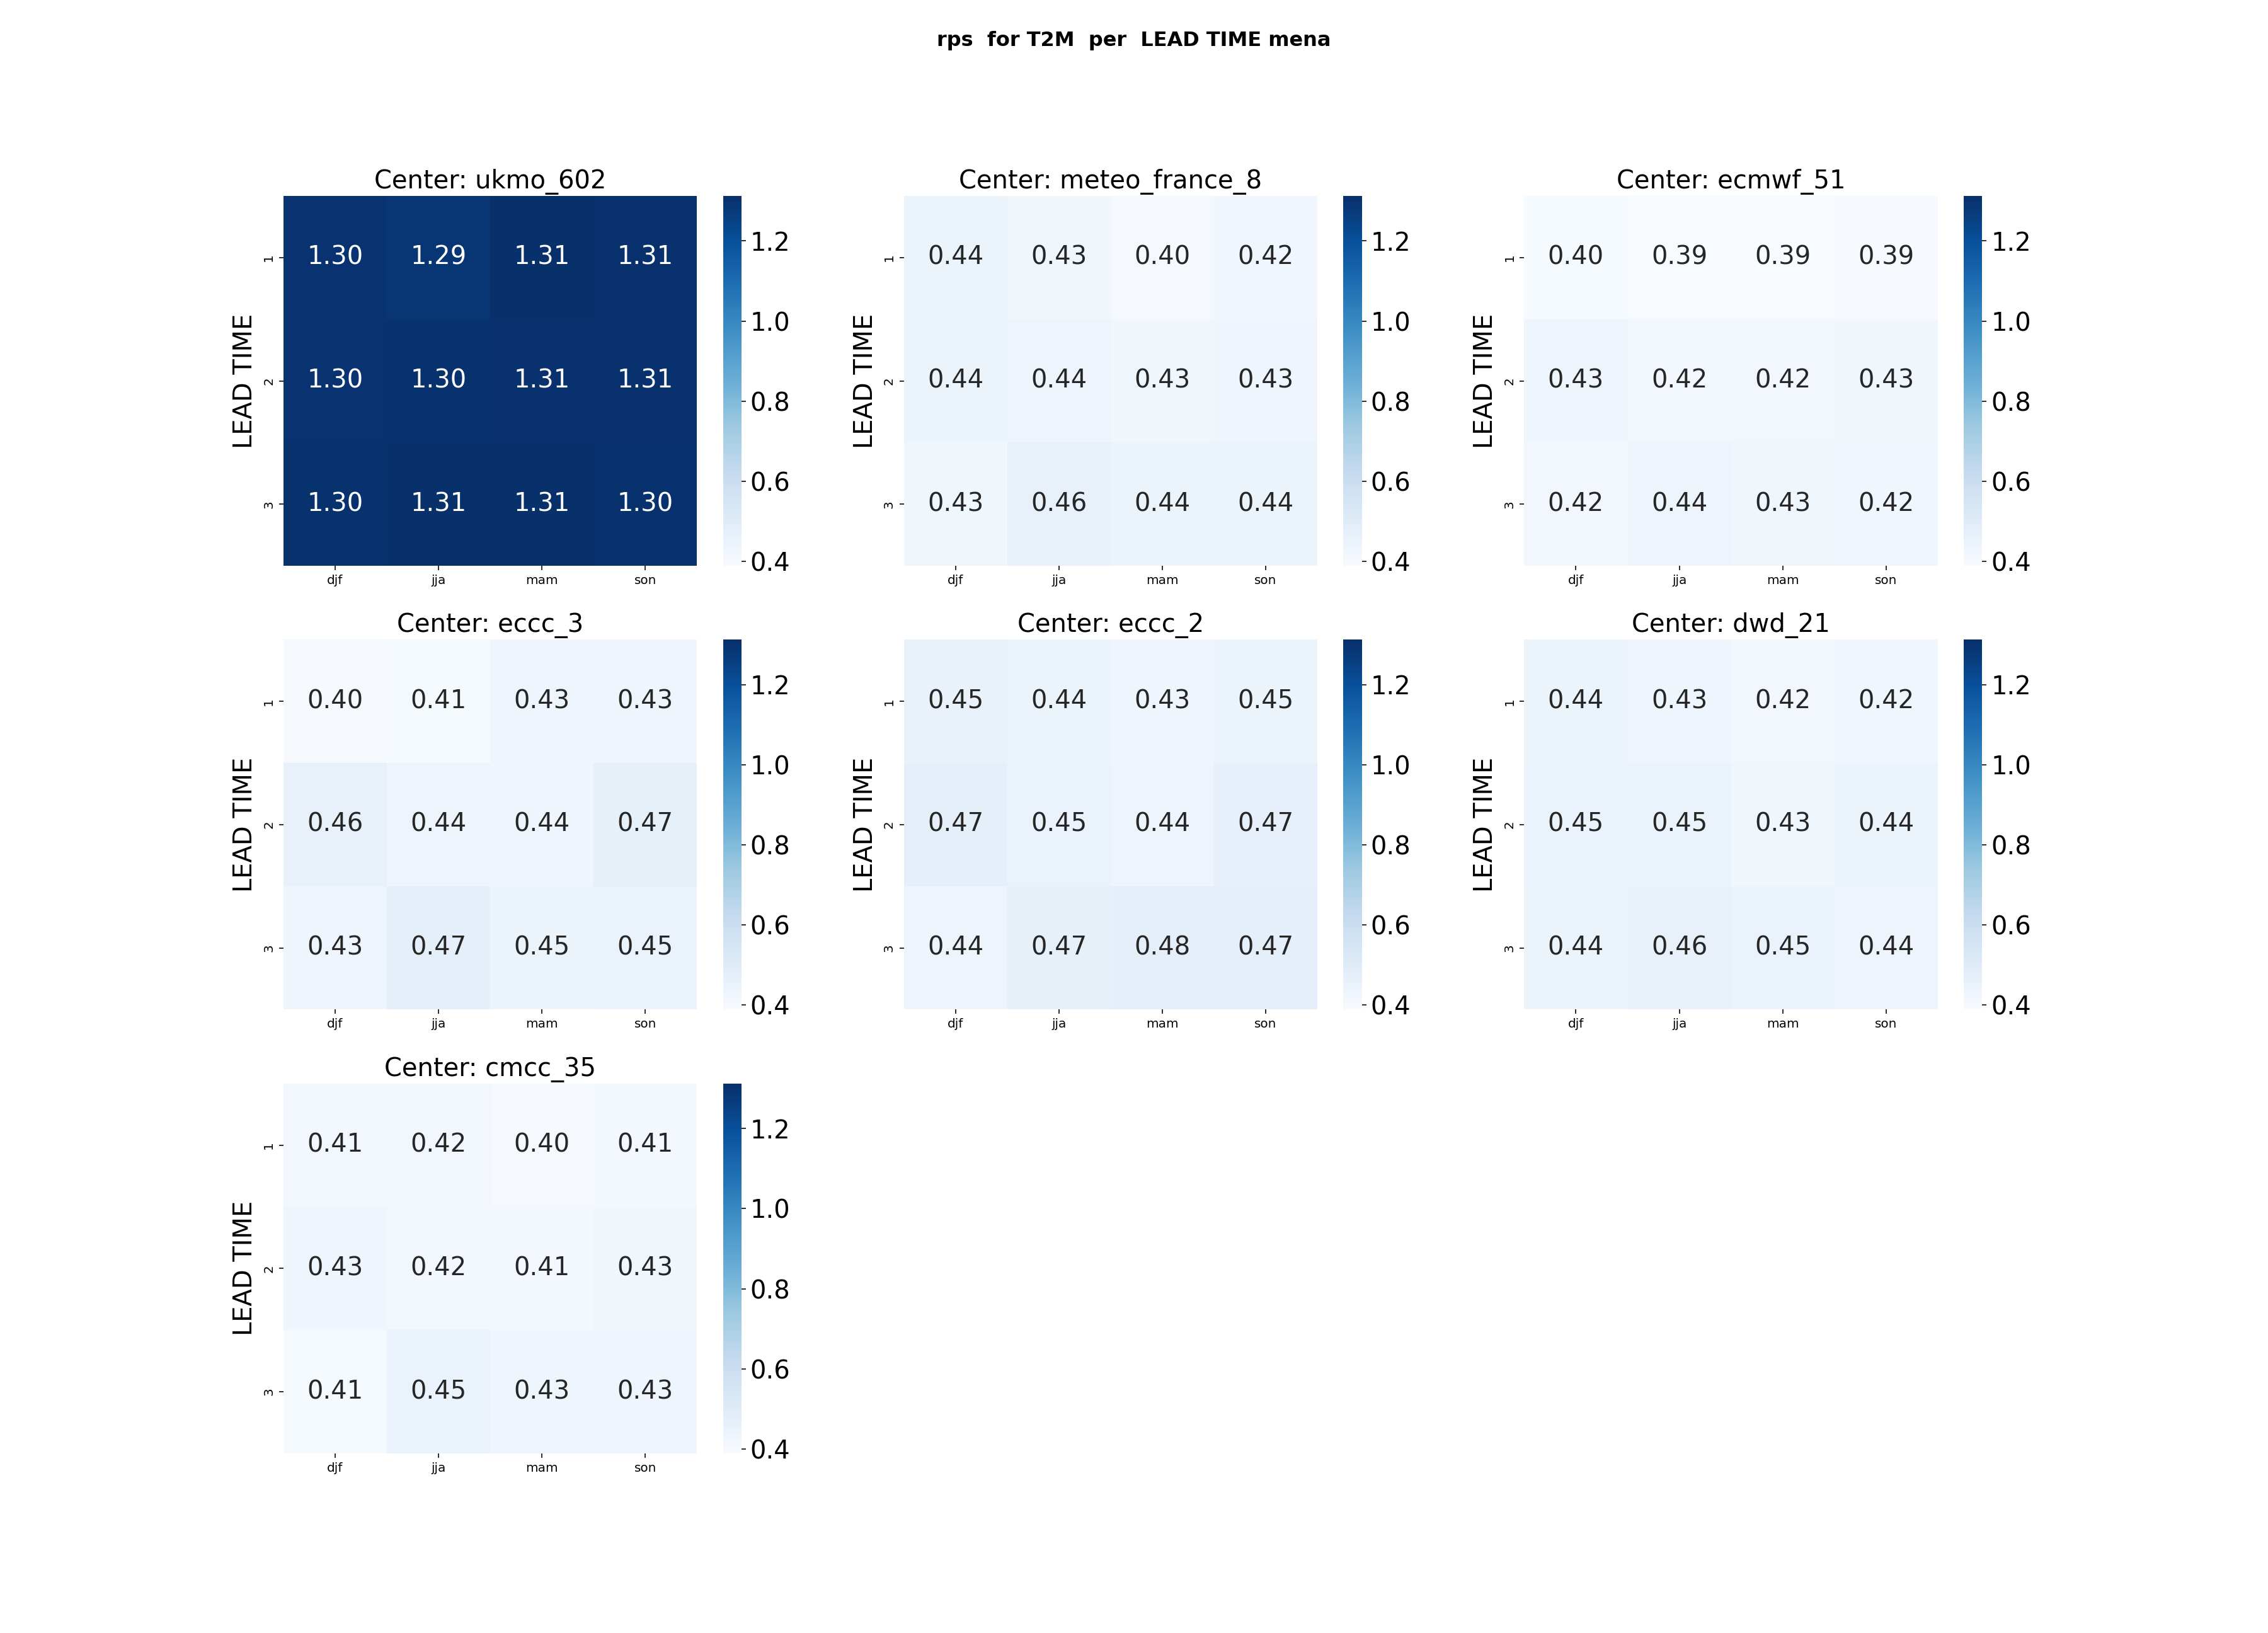
\includegraphics[width=1\linewidth]{plots/prob/rps/rps_T2M_mena.png}
    \caption{Temperature RPS  heatmaps for all the seasons per categories \textbf{\textit{(0 means perfect RPS)}}}
\end{figure}
The figure displaying the Ranked Probability Score (RPS) for different climate models and seasonal periods provides a detailed view of model performance across various start months (DJF, JJA, MAM, SON). Each cell in the matrix represents the RPS value for a specific model and season combination, with the color intensity indicating how well the forecast probabilities match the observed data.

From this figure, it is evident that \textbf{\textit{ECMWF, CMCC-35, METEO-FRANCE and UKMO}}  consistently show lower RPS values, indicating better predictive accuracy across different seasons. This suggests that this forecasts are more closely aligned with observed temperature variability. The relatively higher RPS values for  \textbf{\textit{ECCC}} model underscore their challenges in accurately capturing temperature variations. 

\begin{figure}[H]
    \centering
    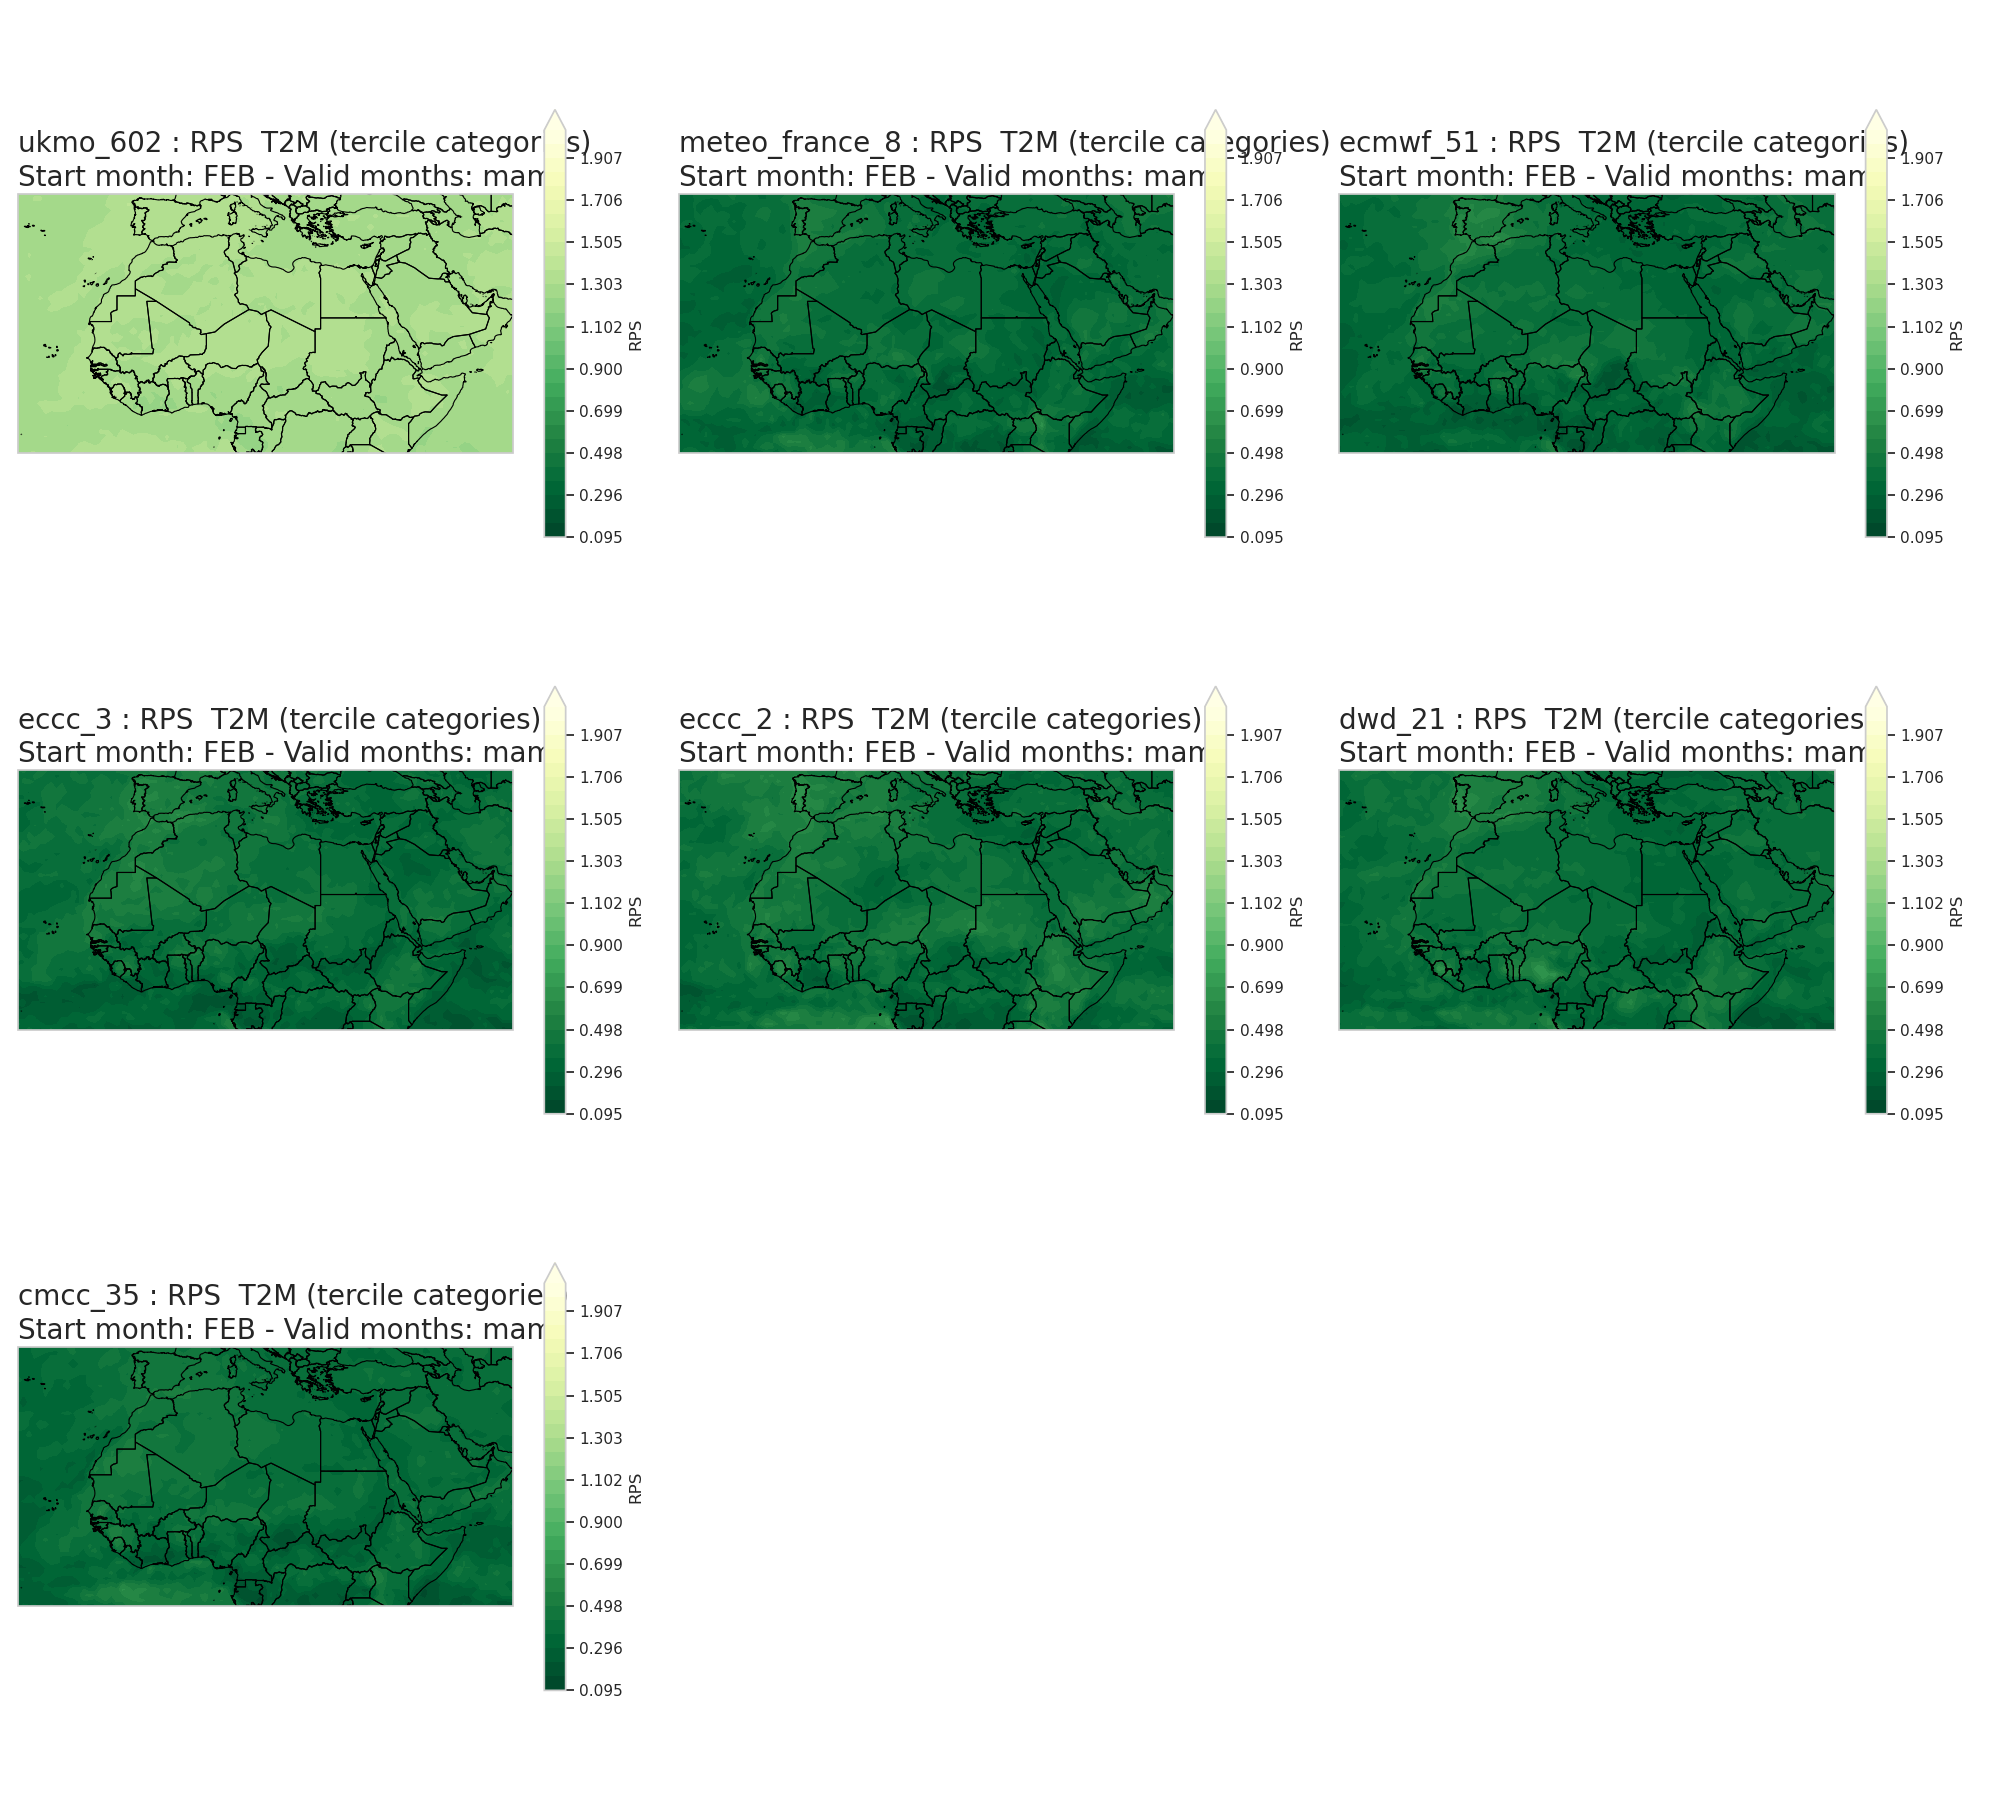
\includegraphics[width=1\linewidth]{plots/prob/rps/rps_mam_t2m.png}
    \caption{Temperature RPS  heatmaps for all the seasons per categories \textbf{\textit{(0 means perfect RPS)}}}
\end{figure}

The figure above illustrates an excellent Ranked Probability Score (RPS), with values approaching 0, which signifies a high degree of accuracy and reliability in the probabilistic forecasts. This indicates that the forecasts effectively capture the uncertainty of outcomes and closely align with observed events.

Moreover, the spatial distribution of the RPS highlights consistent performance across the entire MENA region. The near-uniformity in low RPS values across this extensive and diverse area underscores the robustness of the forecasting system in managing the variability of climatic and weather conditions characteristic of the region.


Overall, the analysis confirms strong forecasting performance in the MENA region, with some variability in accuracy between forecasting centers. The results reinforce the importance of ongoing evaluation and optimization of forecasting systems to ensure consistent and high-quality predictions across all regions.
\paragraph{focus on north africa:}
For the North African region, the results mirror those observed in the broader MENA region.  

This suggests that despite the localized focus on North Africa, the model performance differences remain significant, particularly for \textbf{\textit{ECCC}}. 

\begin{figure}[H]
\includegraphics[scale=0.3]{plots/prob/rps/rps_T2M_NorthAfrica.png}

\caption{Heatmap of T2M  rps  for all centers in North Africa regions}
\end{figure}


\paragraph{focus on Arabian Peninsula}:
All centers exhibit nearly identical performance, with the exception of \textit{ECCC}, which demonstrates lower skill compared to the others.
\subsubsection{Receiver Operating Characteristic}

The ROC (Receiver Operating Characteristic) curve is an important tool for evaluating the performance of predictive models, particularly in the context of probabilistic forecasts. It provides a graphical representation of the trade-off between the true positive rate  and the false positive rate  across various threshold levels.

\begin{figure}[H]
    \centering
    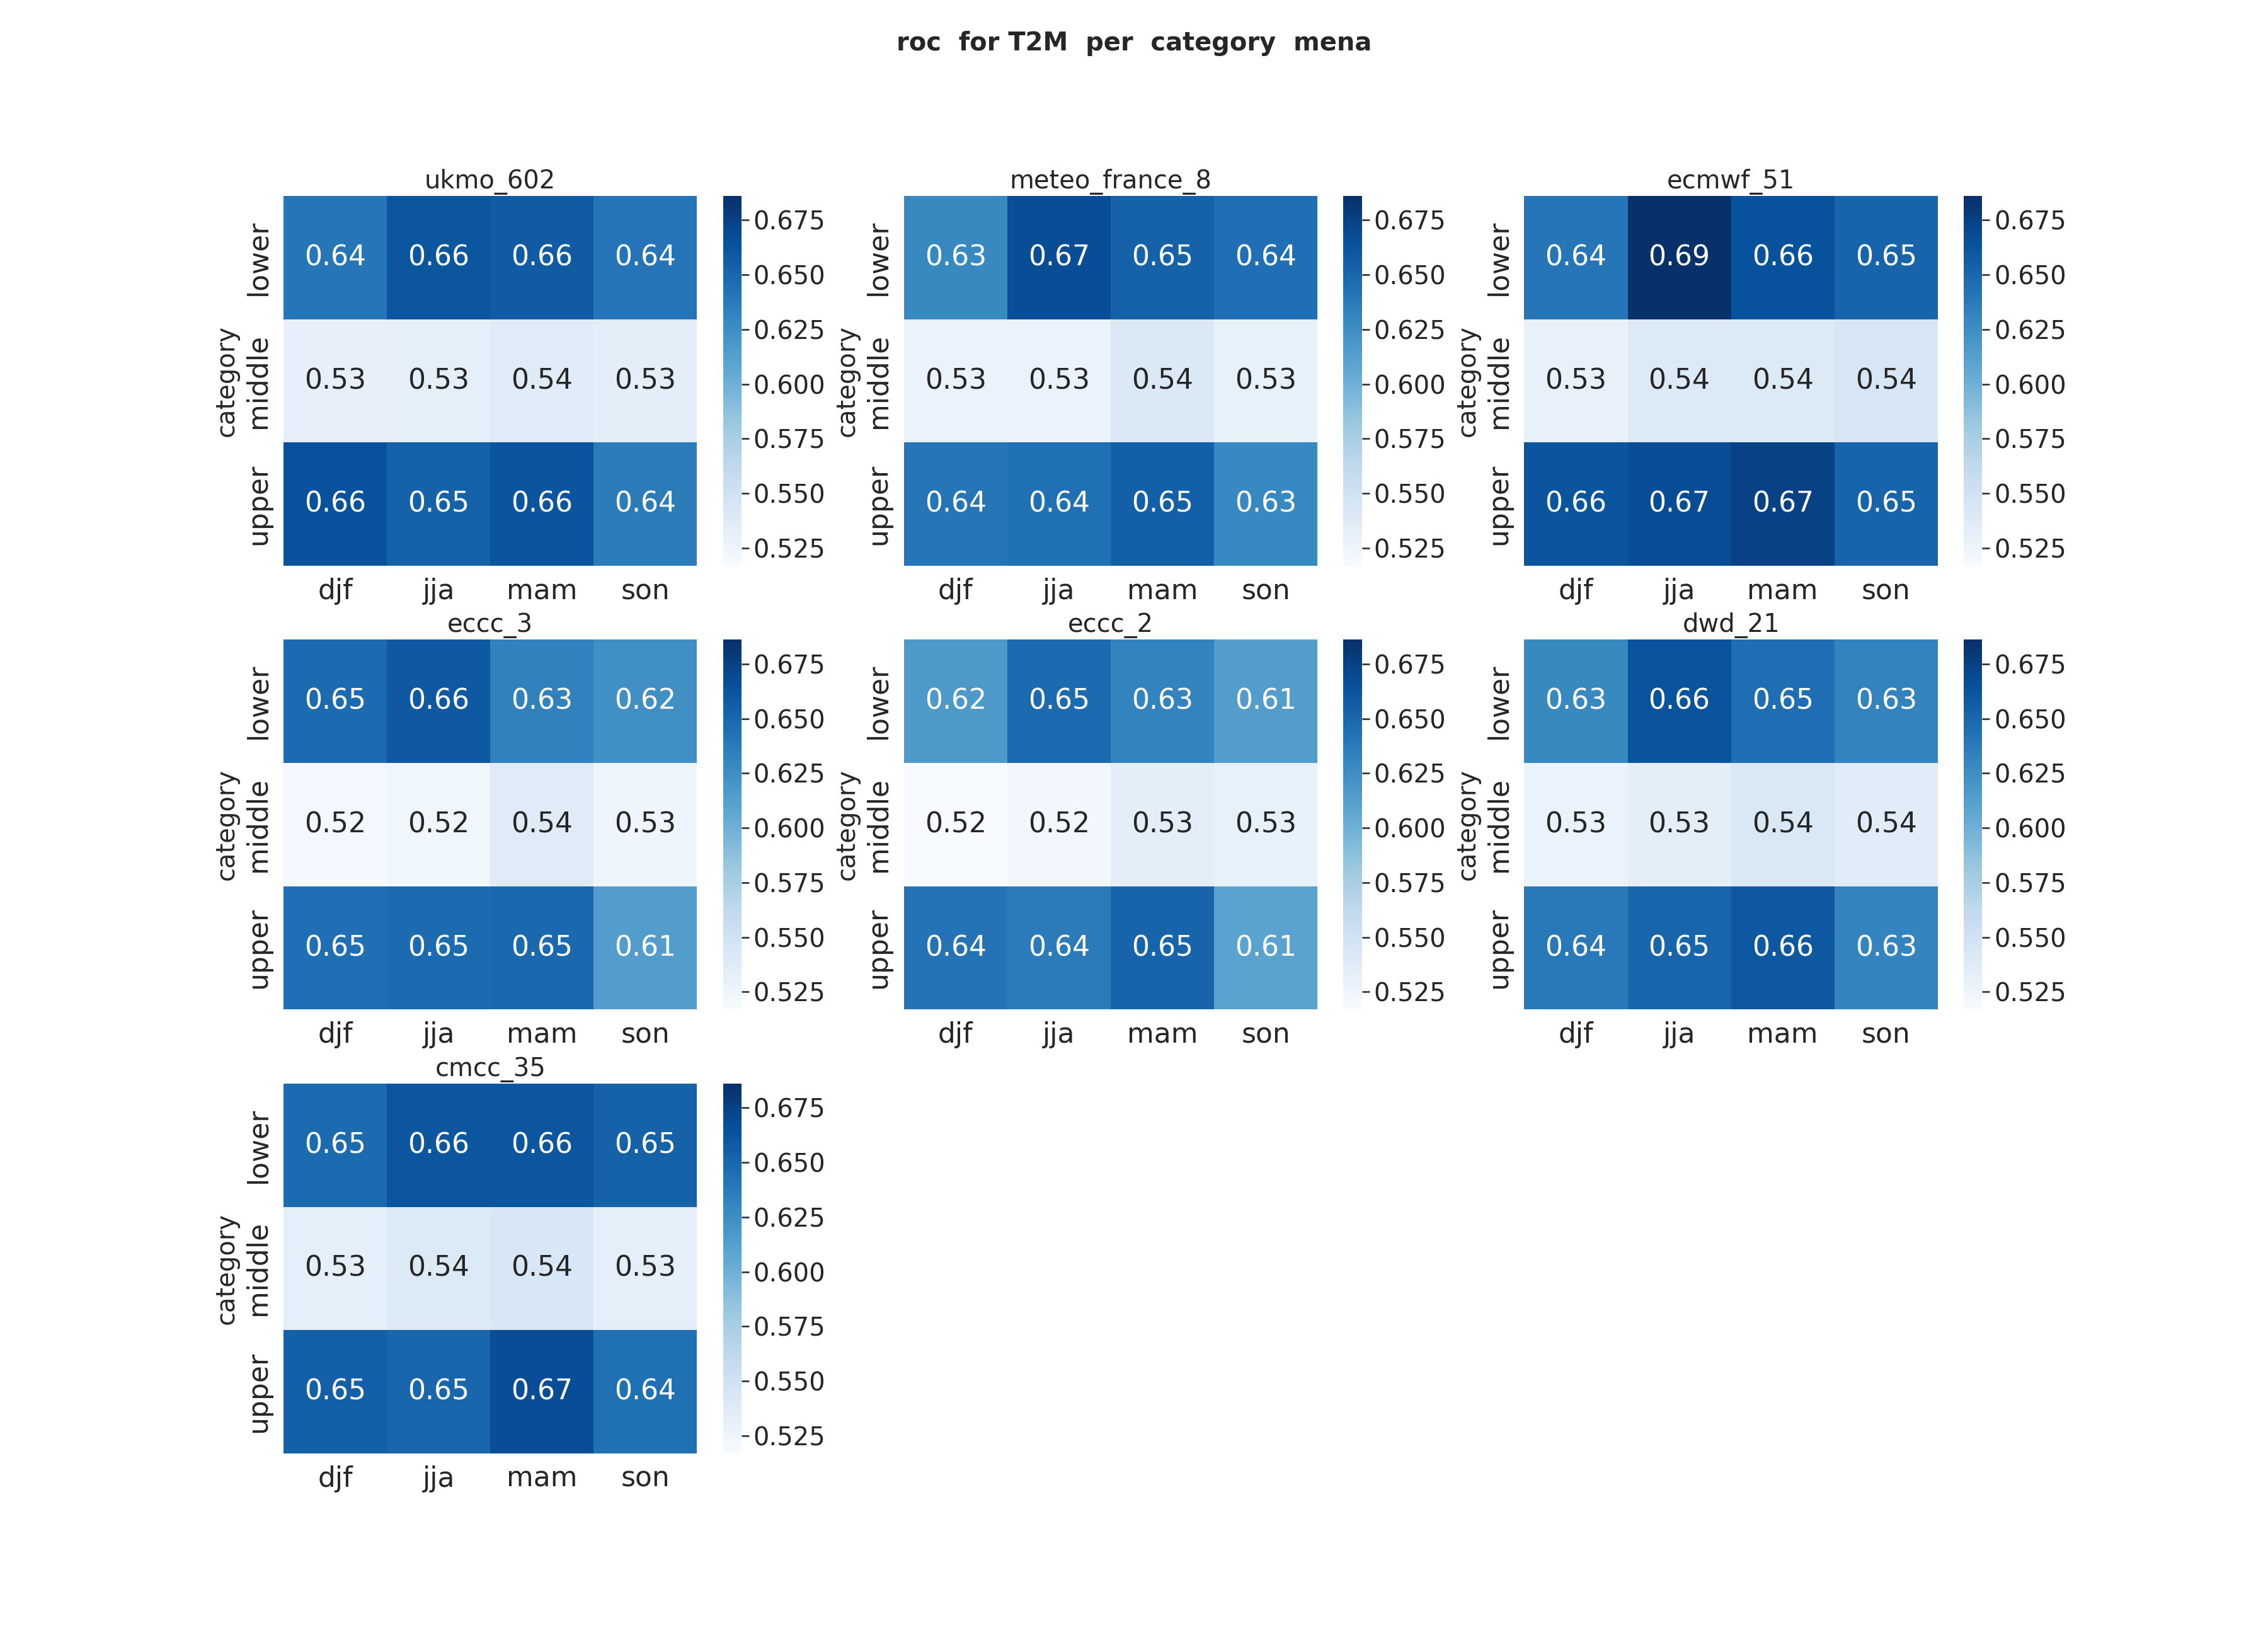
\includegraphics[width=1\linewidth]{plots/prob/roc/roc_T2M_category_mena.png}
    \caption{Temperature AUC  heatmaps \textbf{\textit{(1 means perfect ROC)}}}
\end{figure}


Models generally exhibit similar performance, as indicated by the high Area Under the ROC Curve (AUC) values, which reflect their ability to effectively discriminate between predicted probabilities and observed outcomes. All centers perform relatively well in terms of the AUC, demonstrating good skill in distinguishing between forecasted events and non-events. Similar to the findings with the Brier Score (BS), the "middle" probability category tends to show weaker performance compared to the "lower" and "upper" categories. This highlights the models' greater sensitivity in accurately predicting events with extreme probabilities (high or low), but reduced skill for moderate probability scenarios. This consistency across metrics underscores the need to address forecast performance specifically in the middle category to further improve model predictions.



\begin{figure}[H]
    \centering
    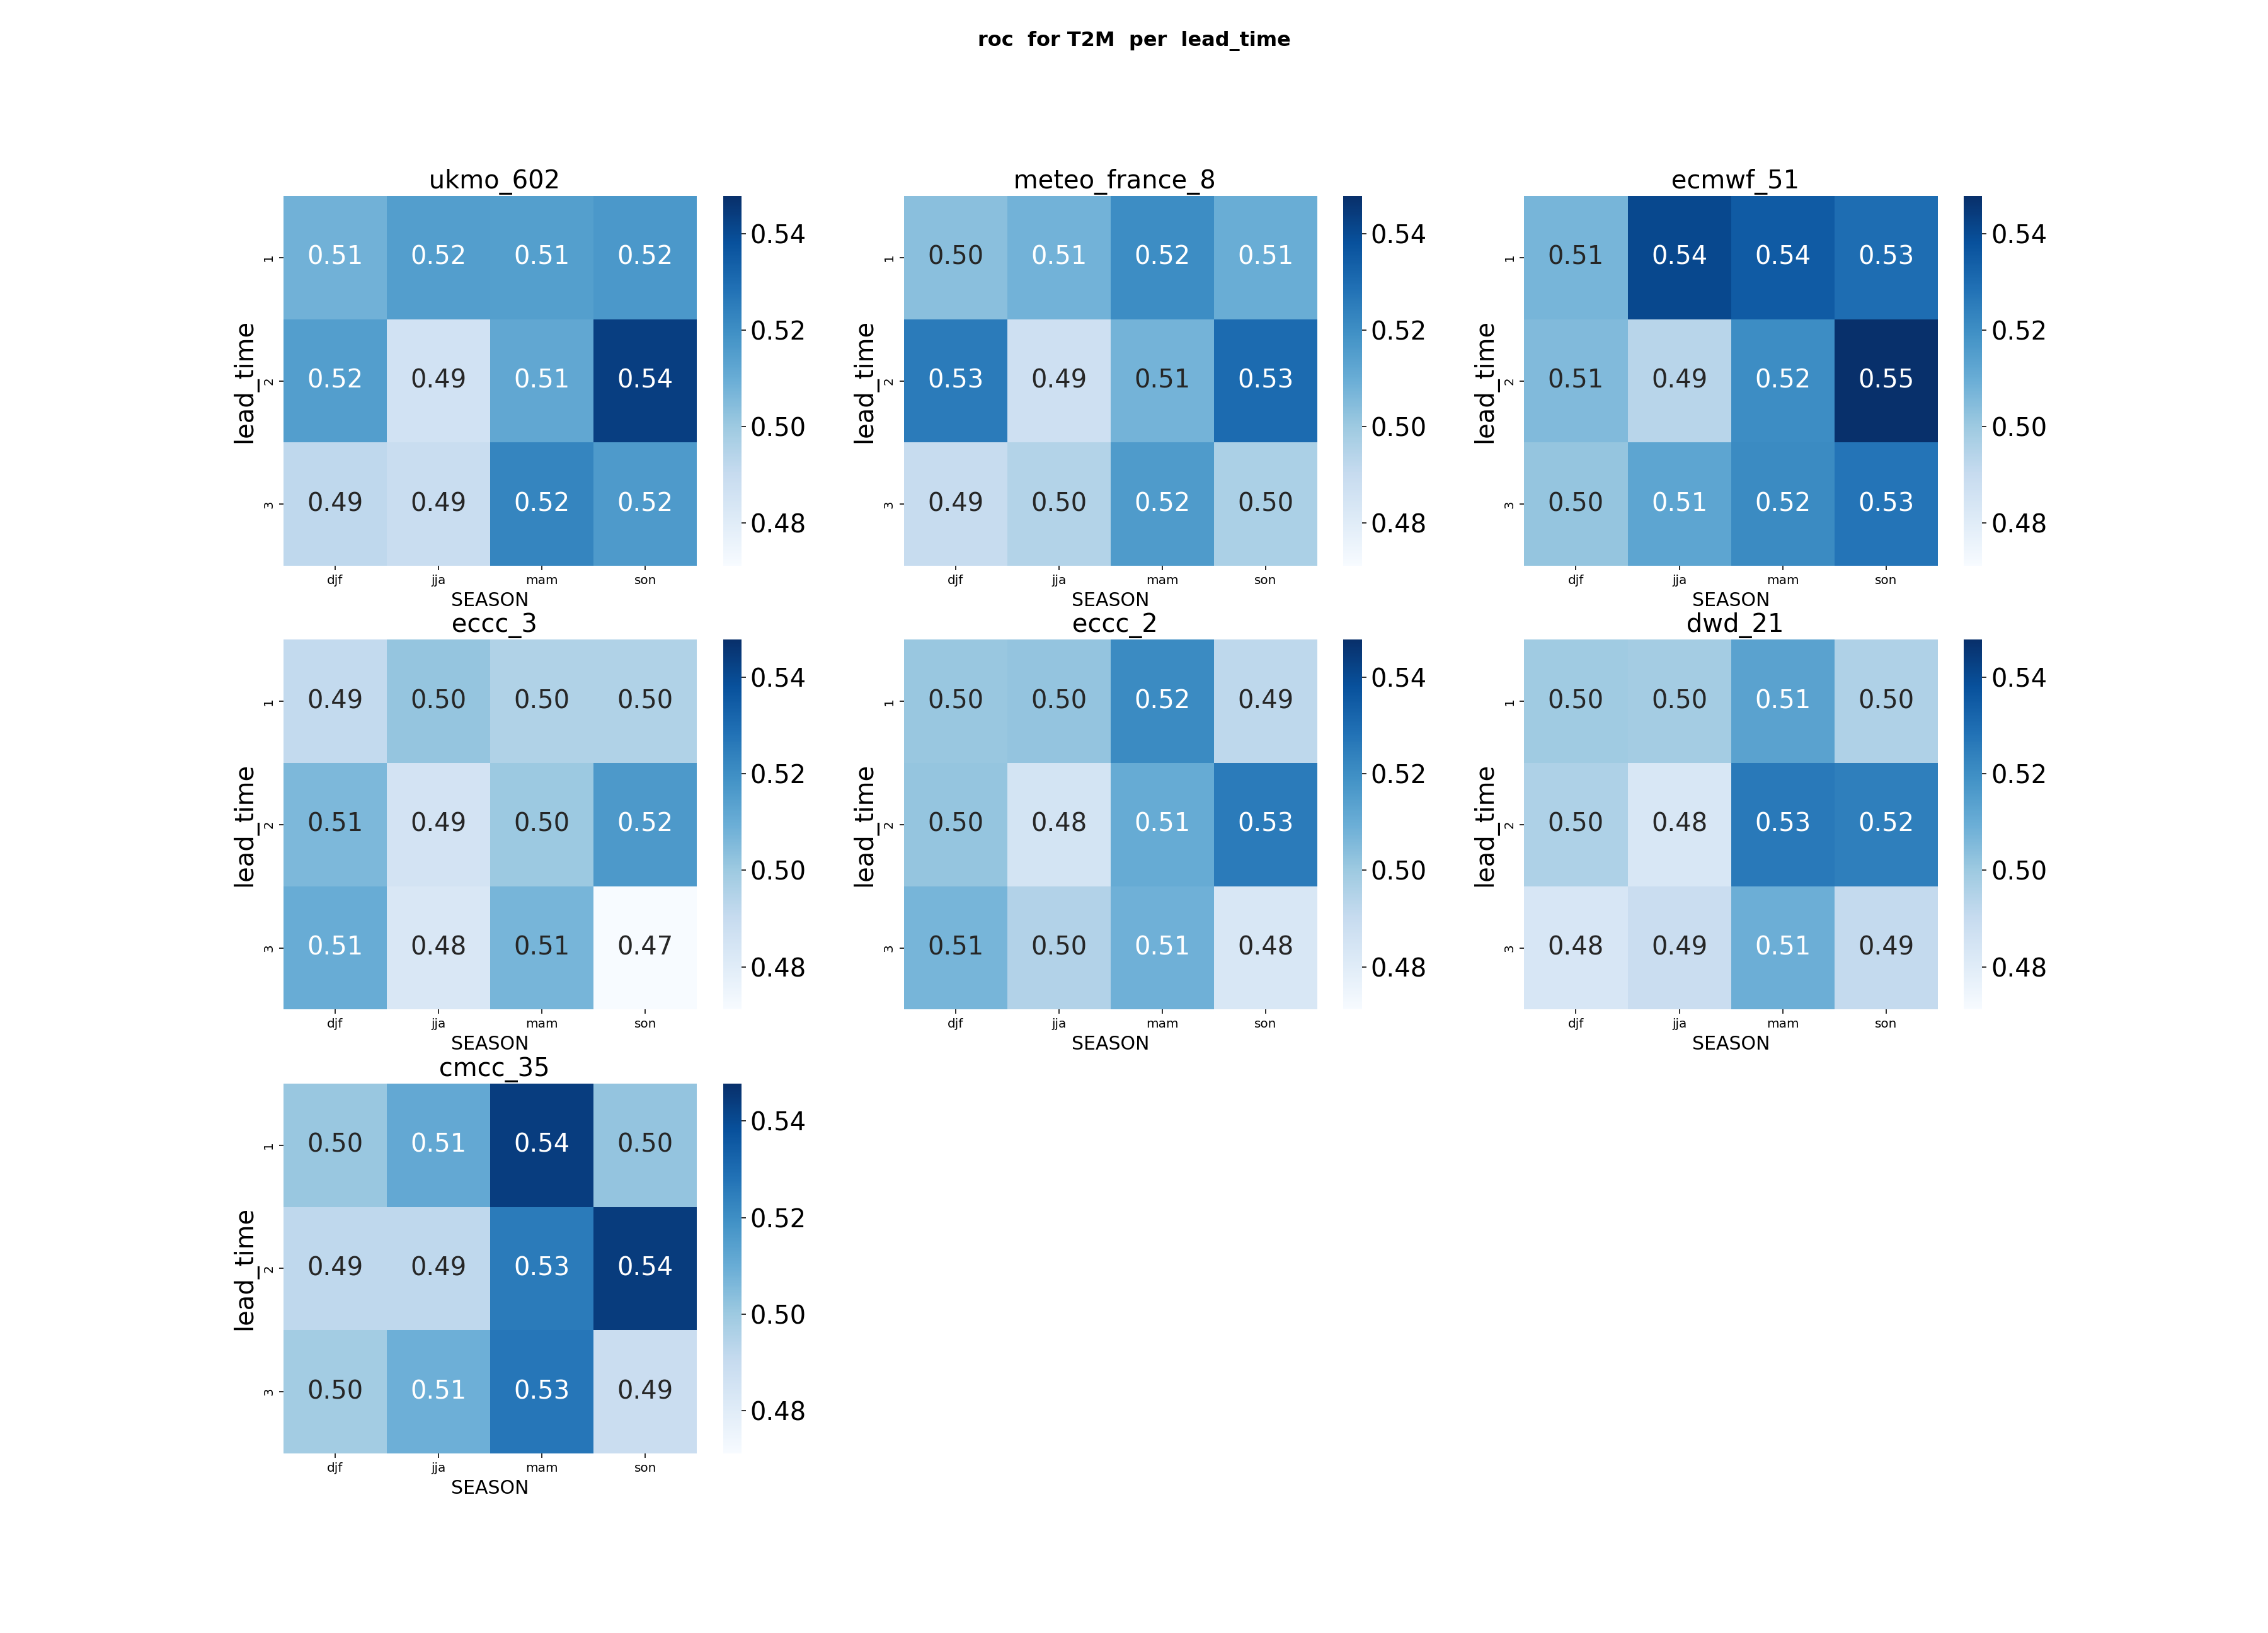
\includegraphics[width=1\linewidth]{plots/prob/roc/roc_T2M_lead_time.png}
    \caption{Temperature AUC  heatmap per lead-time. \textbf{\textit{(1 means perfect ROC)}}}
\end{figure}


The figure above, shows the roc score along lead-time, a noteworthy good performance for SON is observed for the second lead-time, for all centers with values reaching 0.55. As for the other seasons, the performance stay in general stable along lead-time for all centers with scores around 0.5.


\begin{figure}[H]
    \centering
    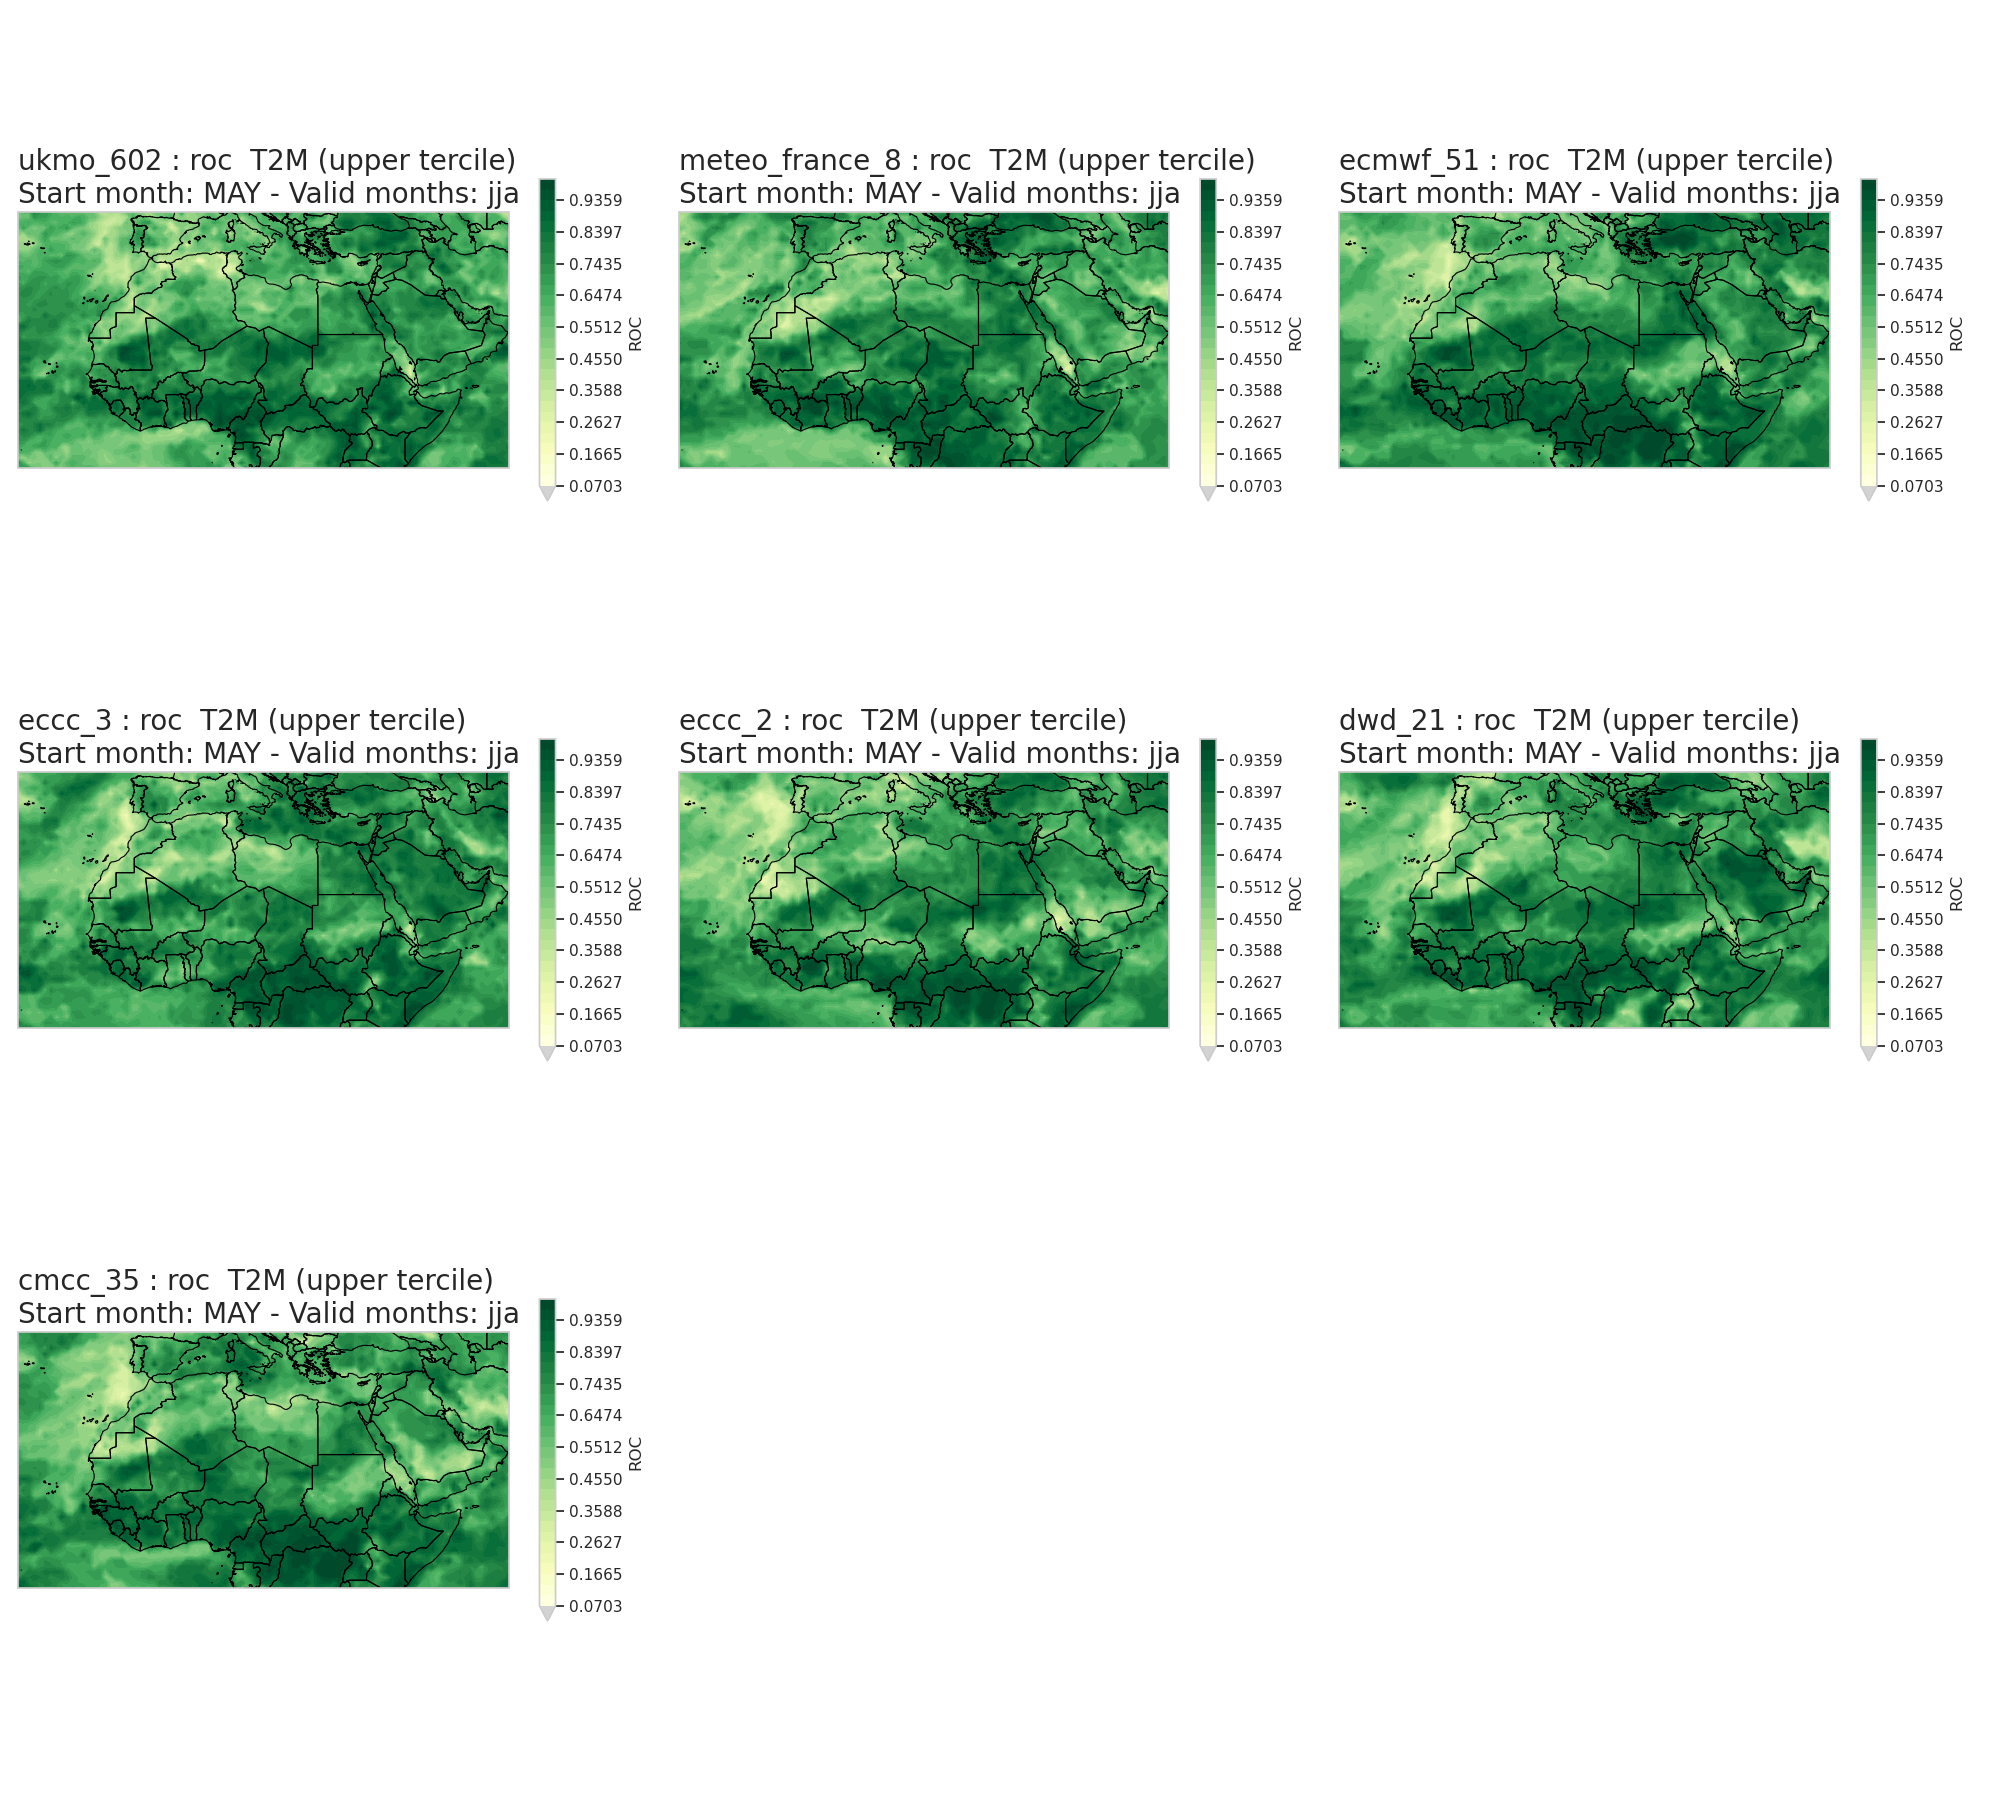
\includegraphics[width=1\linewidth]{plots/prob/roc/roc_jja_t2m_upper.png}
    \caption{2-meter Temperature ROC JJA Upper tercile \textbf{\textit{(1 means perfect ROC)}}}
\end{figure}


\begin{figure}[H]
    \centering
    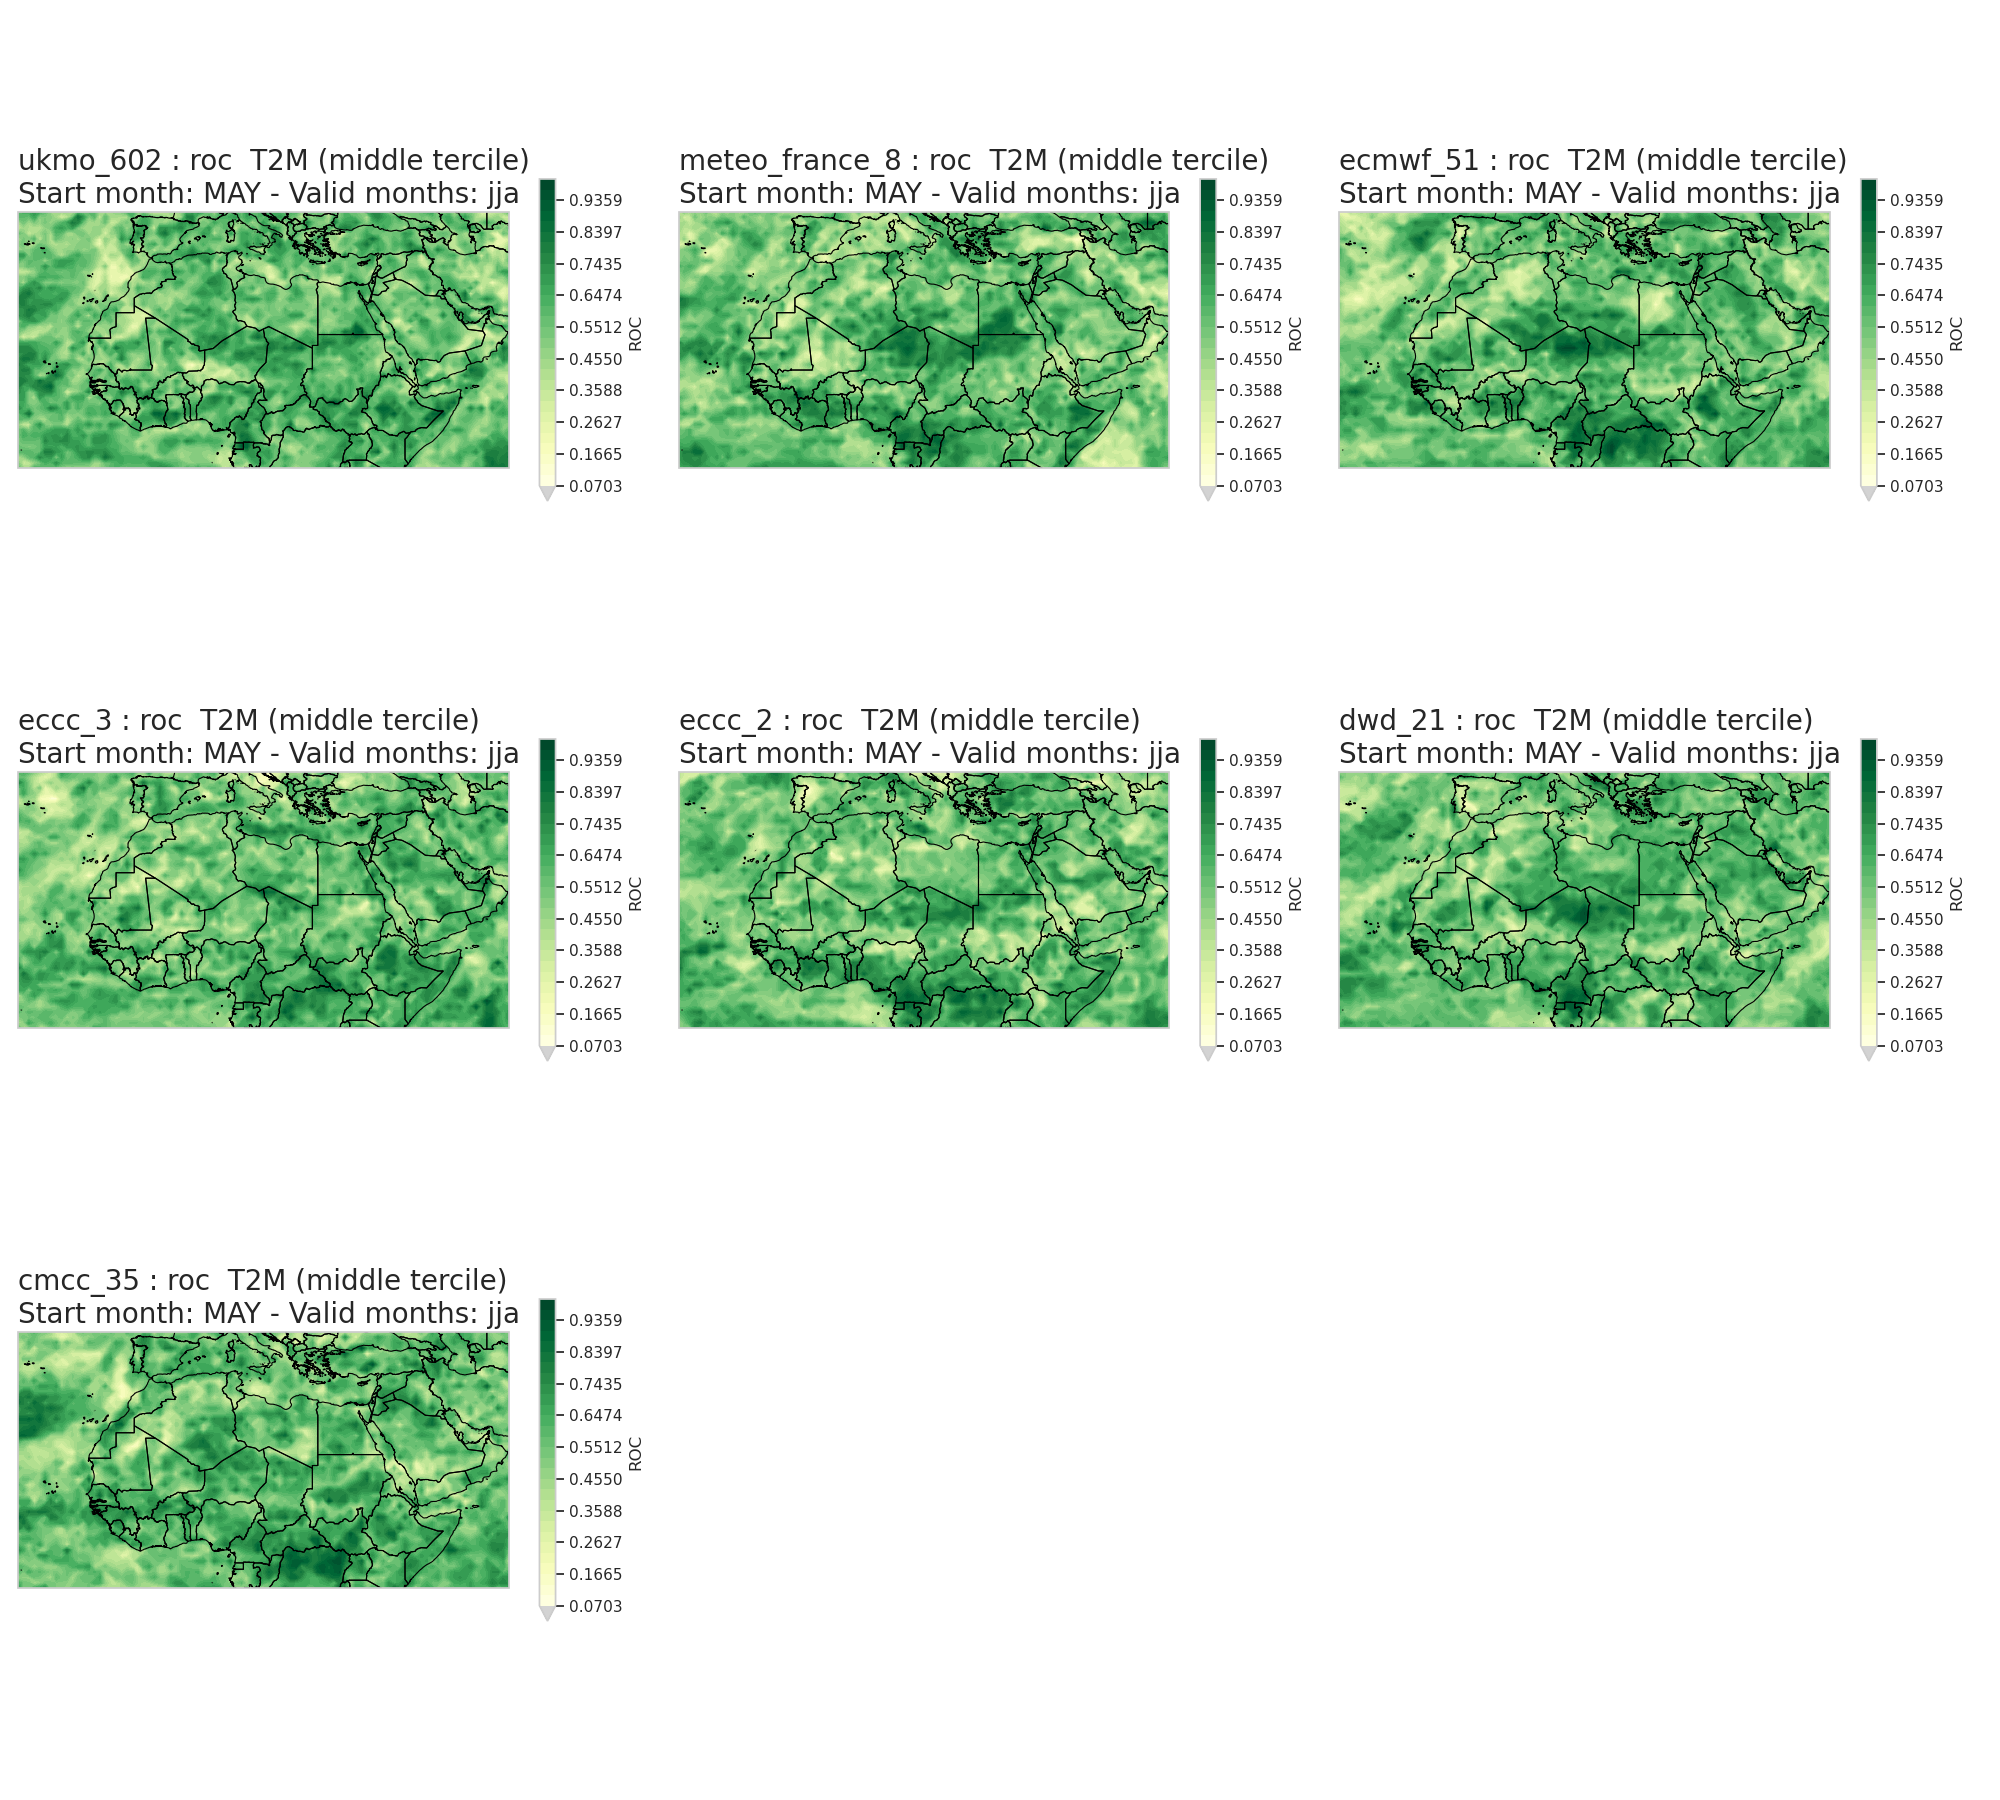
\includegraphics[width=1\linewidth]{plots/prob/roc/roc_jja_t2m_middle.png}
    \caption{2-meter Temperature ROC JJA Middle tercile \textbf{\textit{(1 means perfect ROC)}}}
\end{figure}

For the Upper tercile, the analysis of the spacial variation of ROC score (AUC), shows excellent scores for all scores especially \textbf{\textit{ECMWF}}. The spacial distribution shows a quite variation in North Africa. Thus, the \textbf{\textit{DWD}} exhibit the best performance for Arabian peninsula. Hence, the discrimination (Ability to distinguish
events from non-events) is good for the upper tercile as well as for the lower tercile.

As for the Middle tercile, the performance is much lower. The spacial variability is very high and there is no clear pattern of the score, reflecting a week discrimination for the middle tercile. Thus, the discrimination of extreme events (lower and above normal) is much better than the normal situations.

\paragraph{focus on north africa:}



\begin{figure}[H]
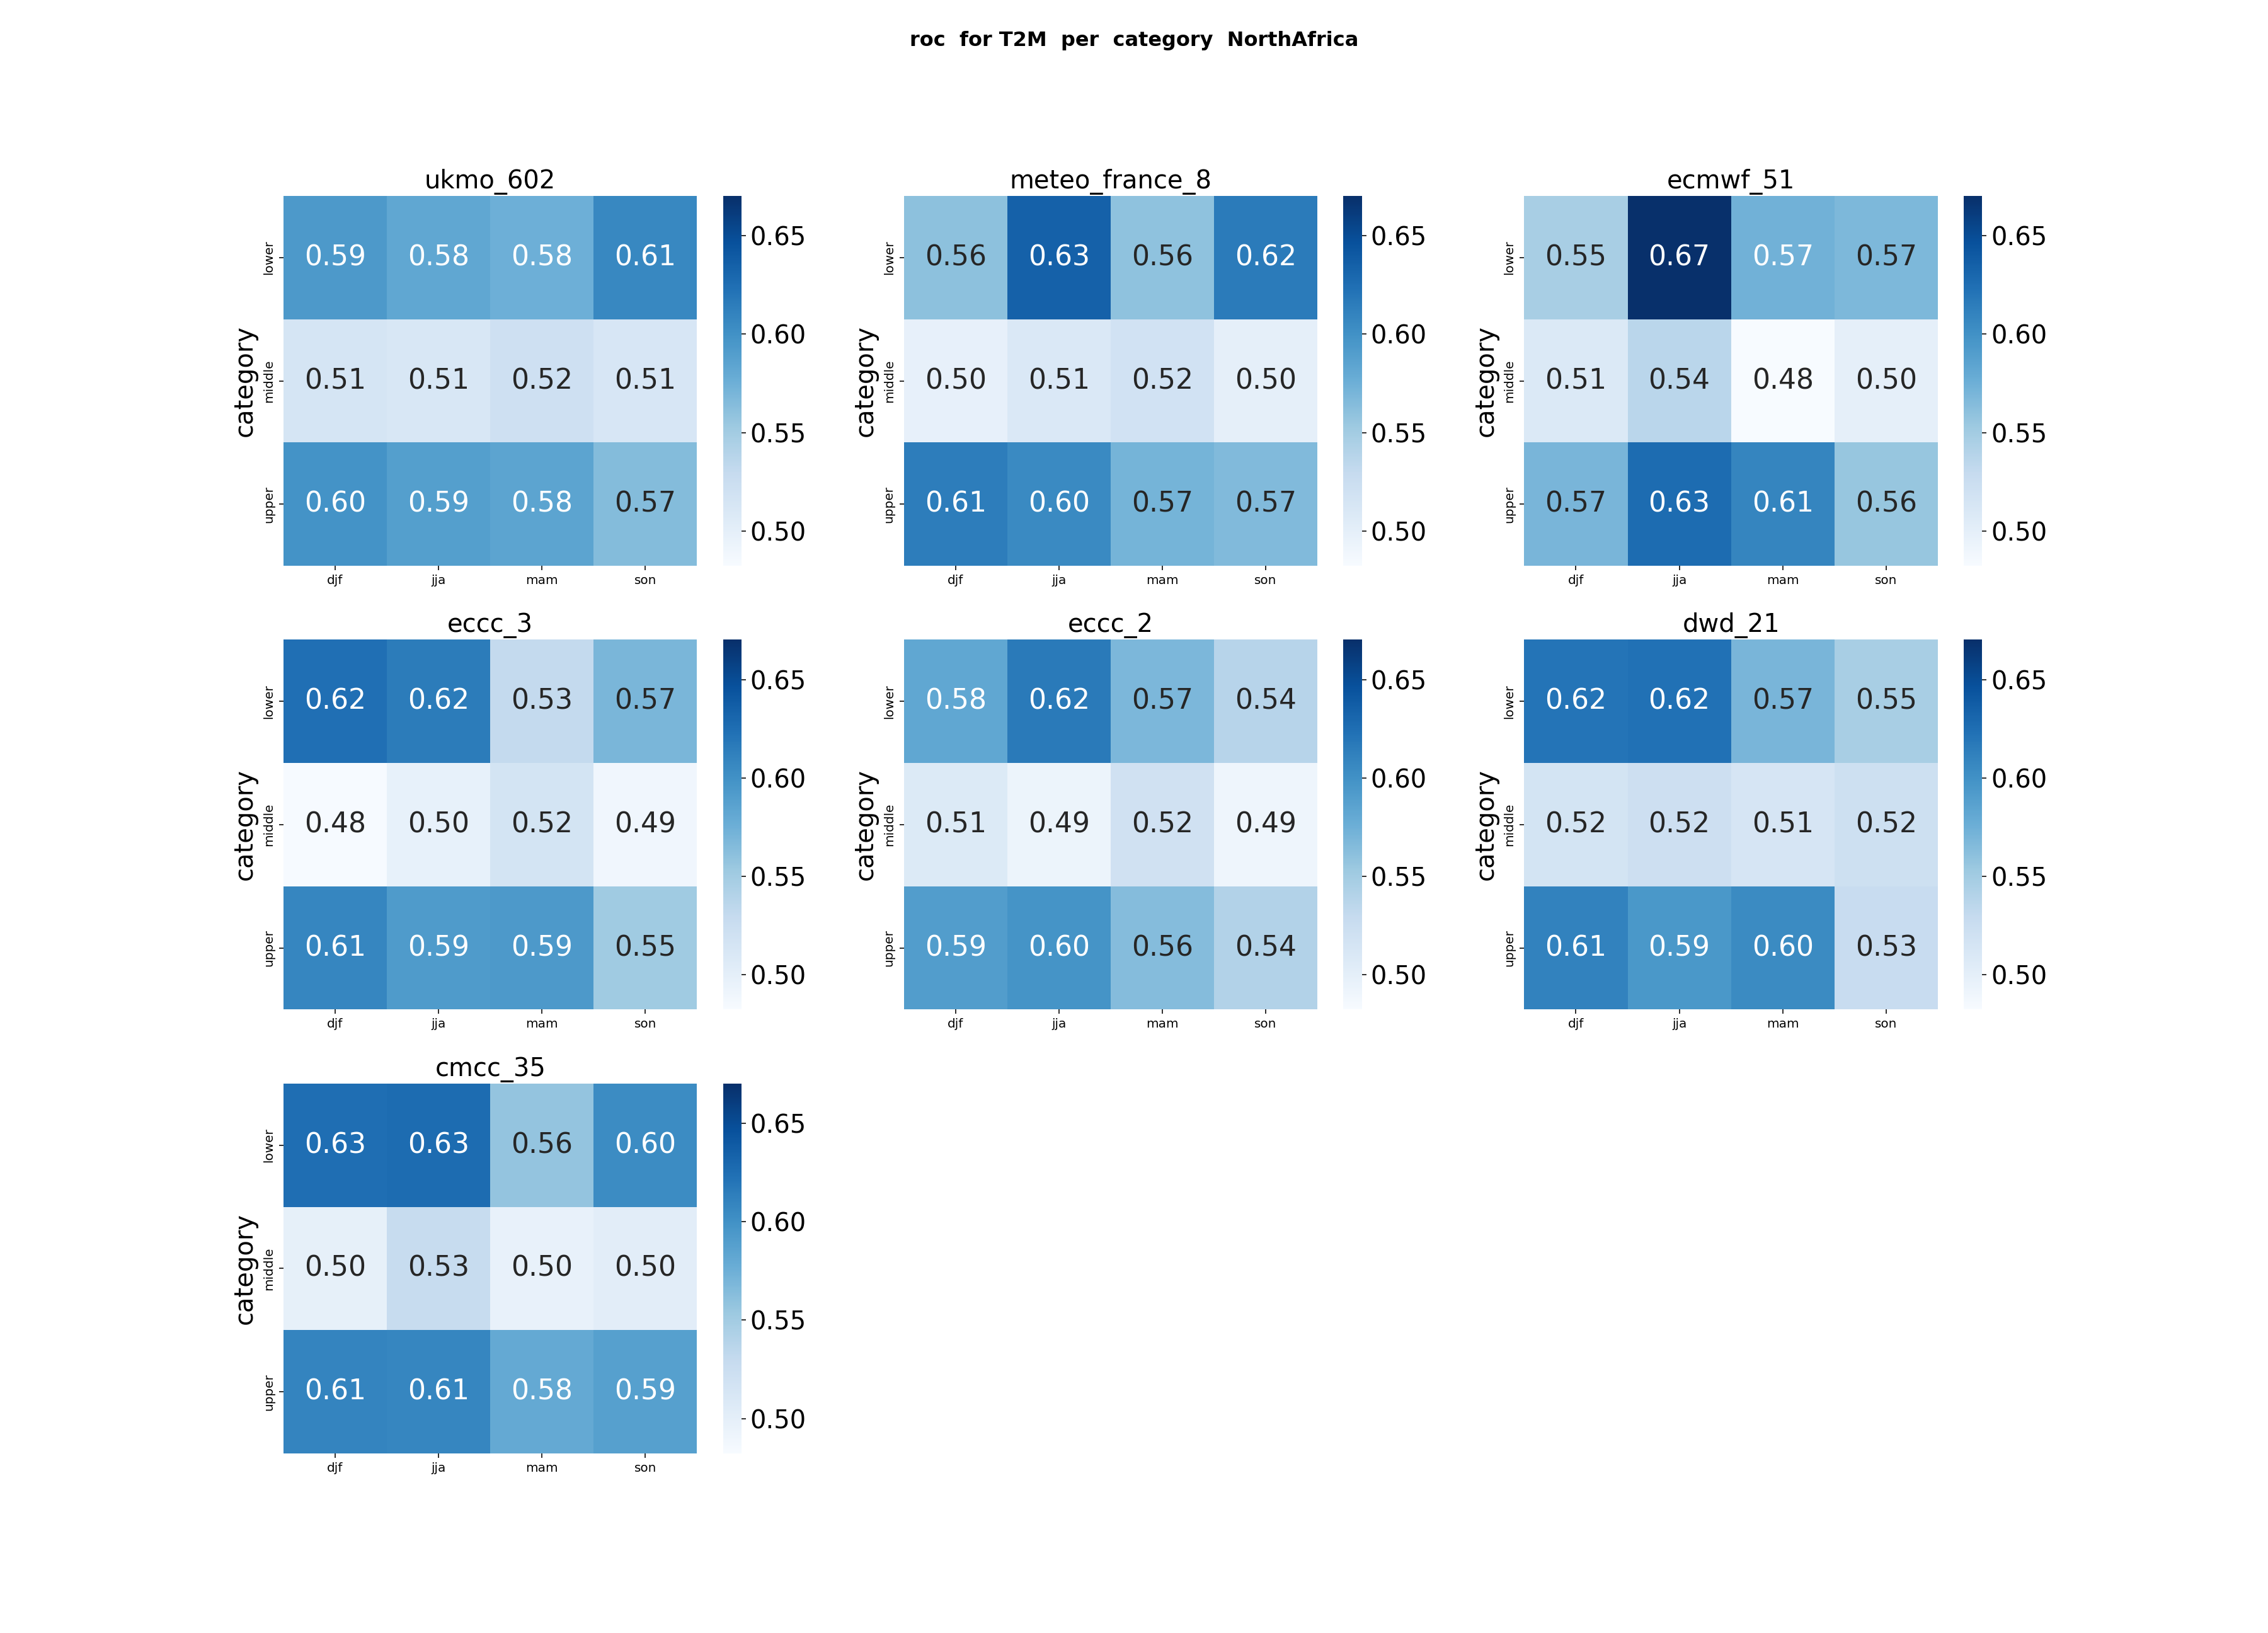
\includegraphics[scale=0.3]{plots/prob/roc/roc_T2M_category_NorthAfrica.png}
\caption{Temperature AUC  heatmaps for north africa }
\end{figure}

The figure above confirms the same conclusions for the North Africa region. The models generally maintain similar performance, with high AUC values reflecting strong discrimination skill across all categories. The UKMO continues to show robust results in terms of ROC. As observed previously, the "middle" probability category remains the least performant compared to the "lower" and "upper" categories, indicating the models' reduced ability to predict moderate probability events. This consistency in findings suggests that the regional focus on North Africa does not significantly alter the overall assessment of model performance.
\paragraph{focus on Arabian Peninsula}:
There are no significant differences in performance across the centers, indicating comparable skill levels.

\subsubsection{Relative operating characteristics Skill Score}
ROCSS provides an assessment of a model's ability to discriminate between observed and forecasted events relative to a reference model, often a climatological or random forecast. A higher ROCSS indicates that the model has skill in distinguishing between occurrences and non-occurrences of an event, while a score close to zero suggests no significant improvement over the reference.

\begin{figure}[H]
    \centering
    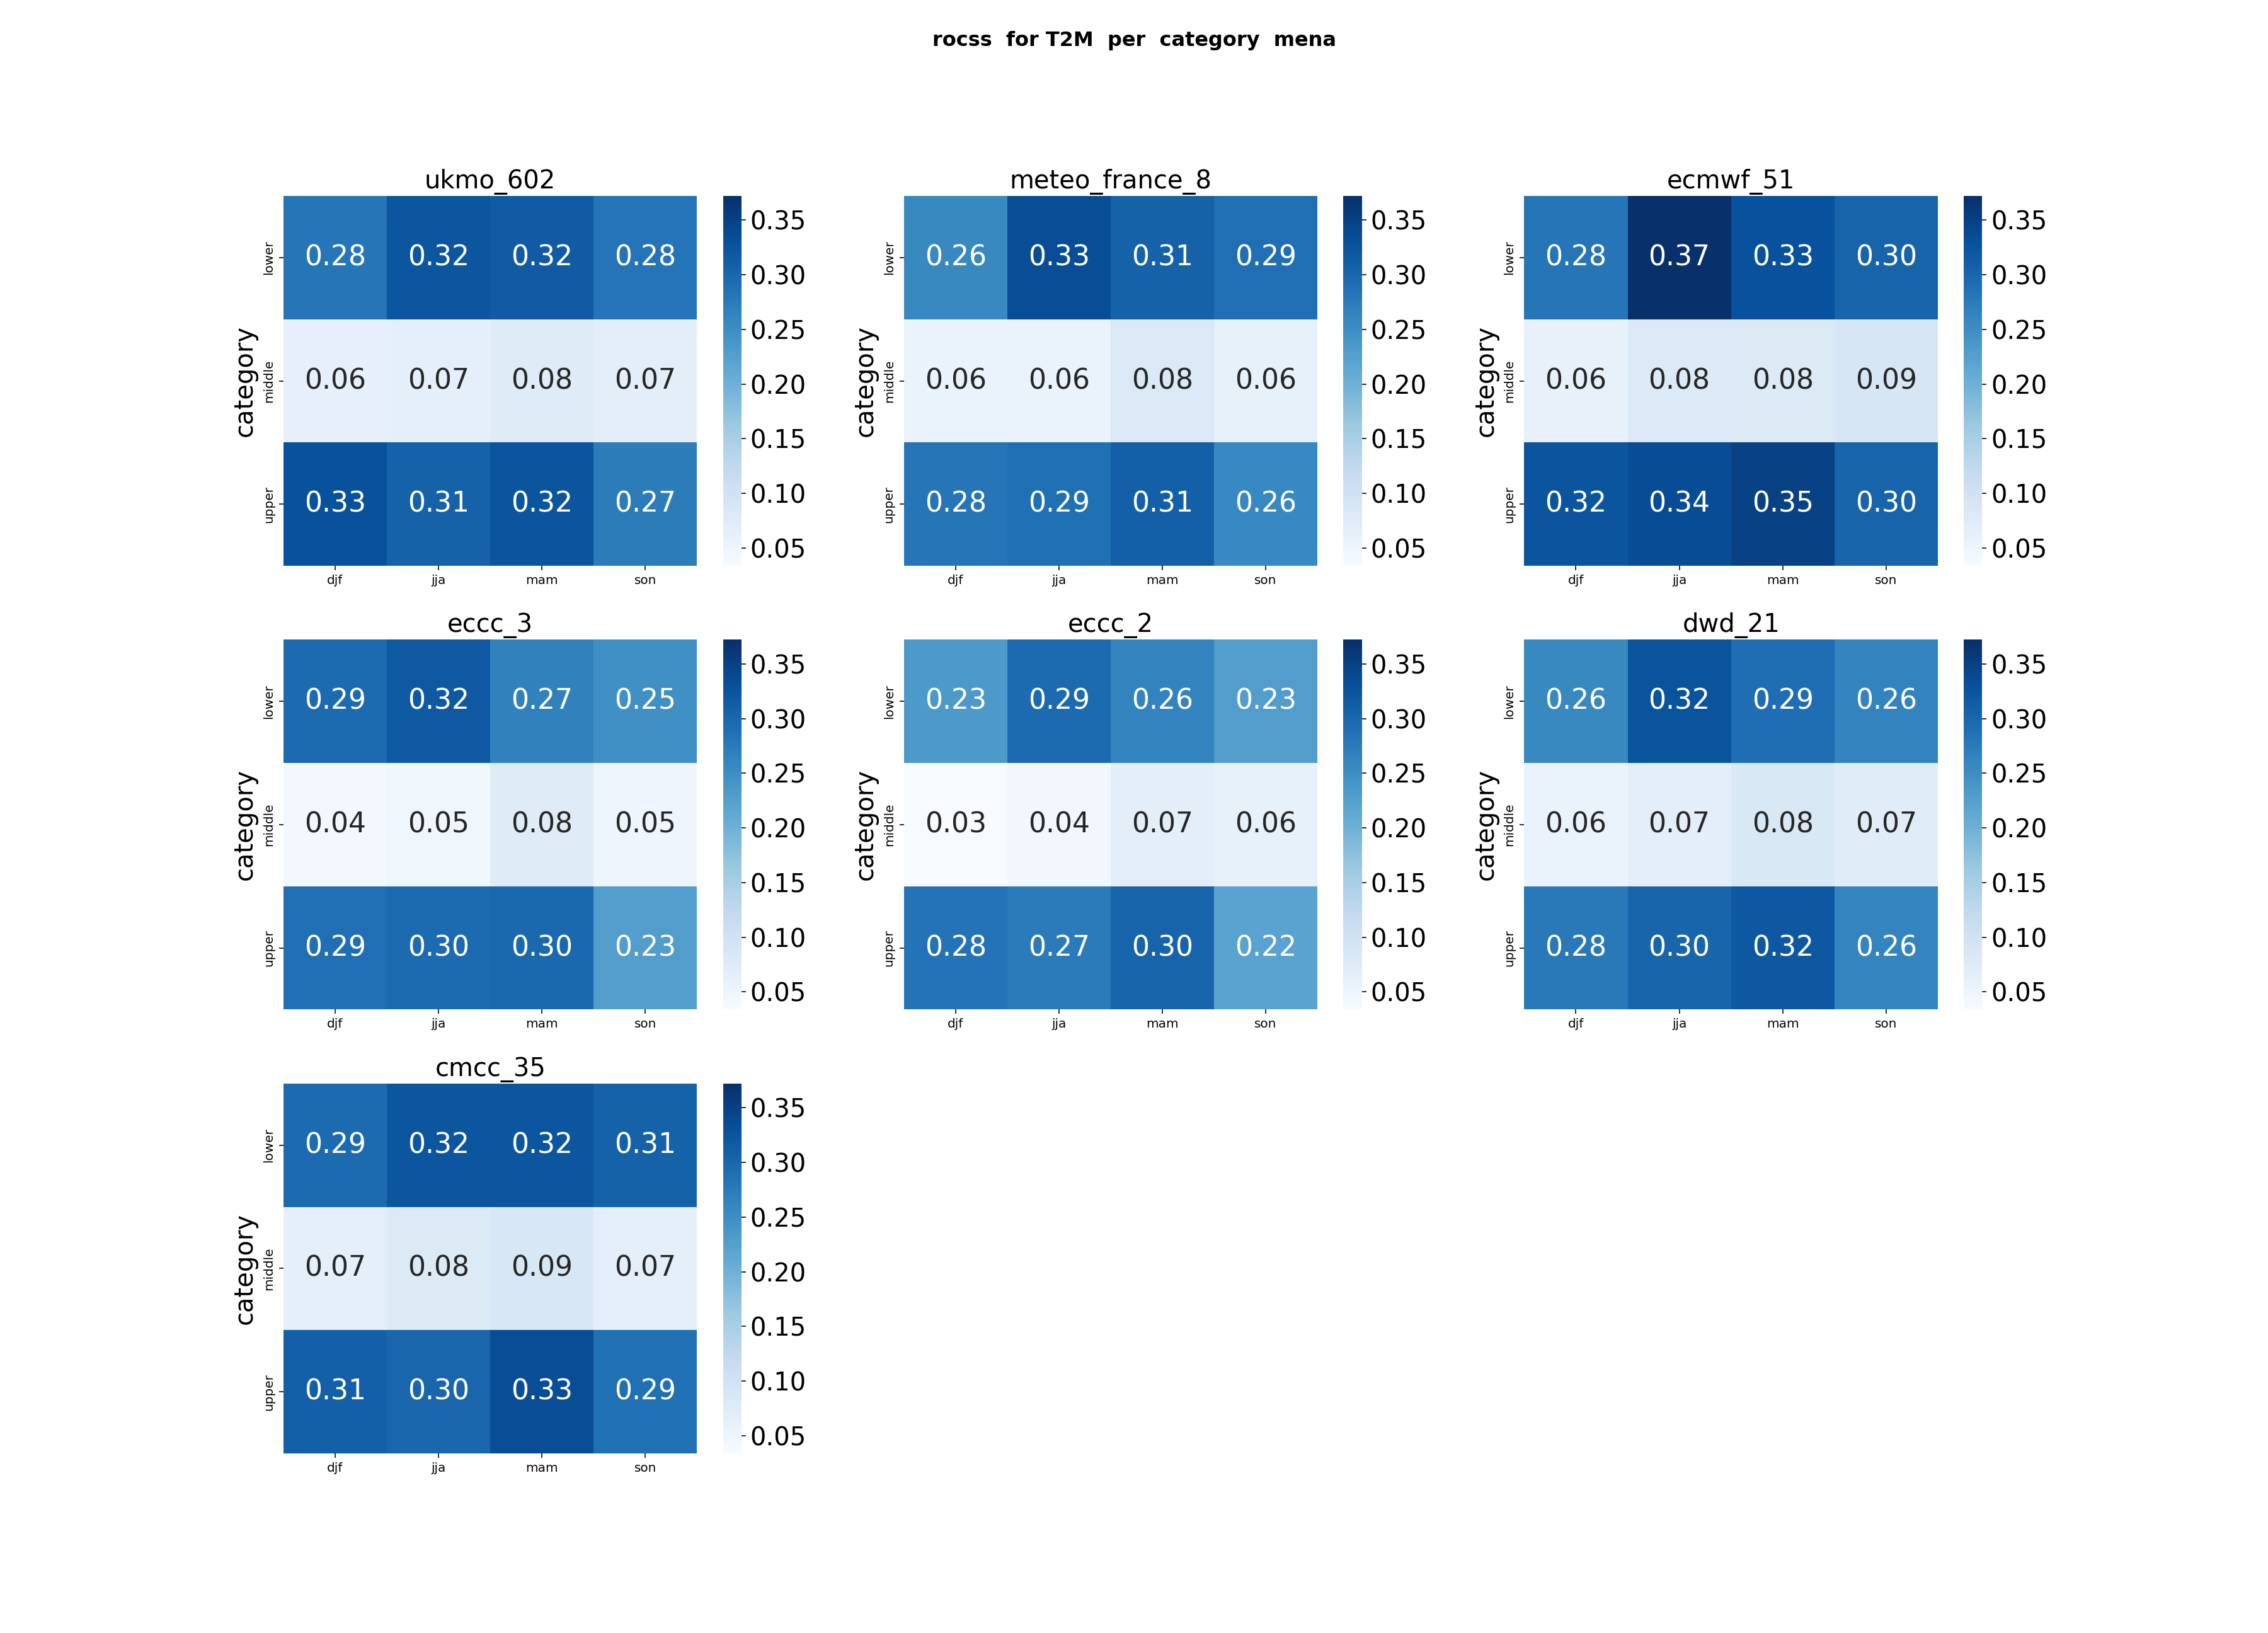
\includegraphics[width=1\linewidth]{plots/prob/rocss/rocss_T2M_category_mena.png}
    \caption{Temperature ROCSS  heatmaps for MENA region per category \textbf{\textit{(1 means perfect ROCSS)}} }
\end{figure}
The models generally demonstrate consistent and positive skill, highlighting their ability to discriminate between observed and forecasted events. UKMO, which showed good performance in reliability metrics, continues to perform well in terms of ROCSS, confirming its relative robustness in event discrimination. Additionally, as observed with the ROC scores, the "middle" category exhibits lower performance compared to the "lower" and "upper" categories. This indicates that while the models excel at predicting extreme events with high or low probabilities, their ability to capture moderate probability events remains limited.

\begin{figure}[H]
    \centering
    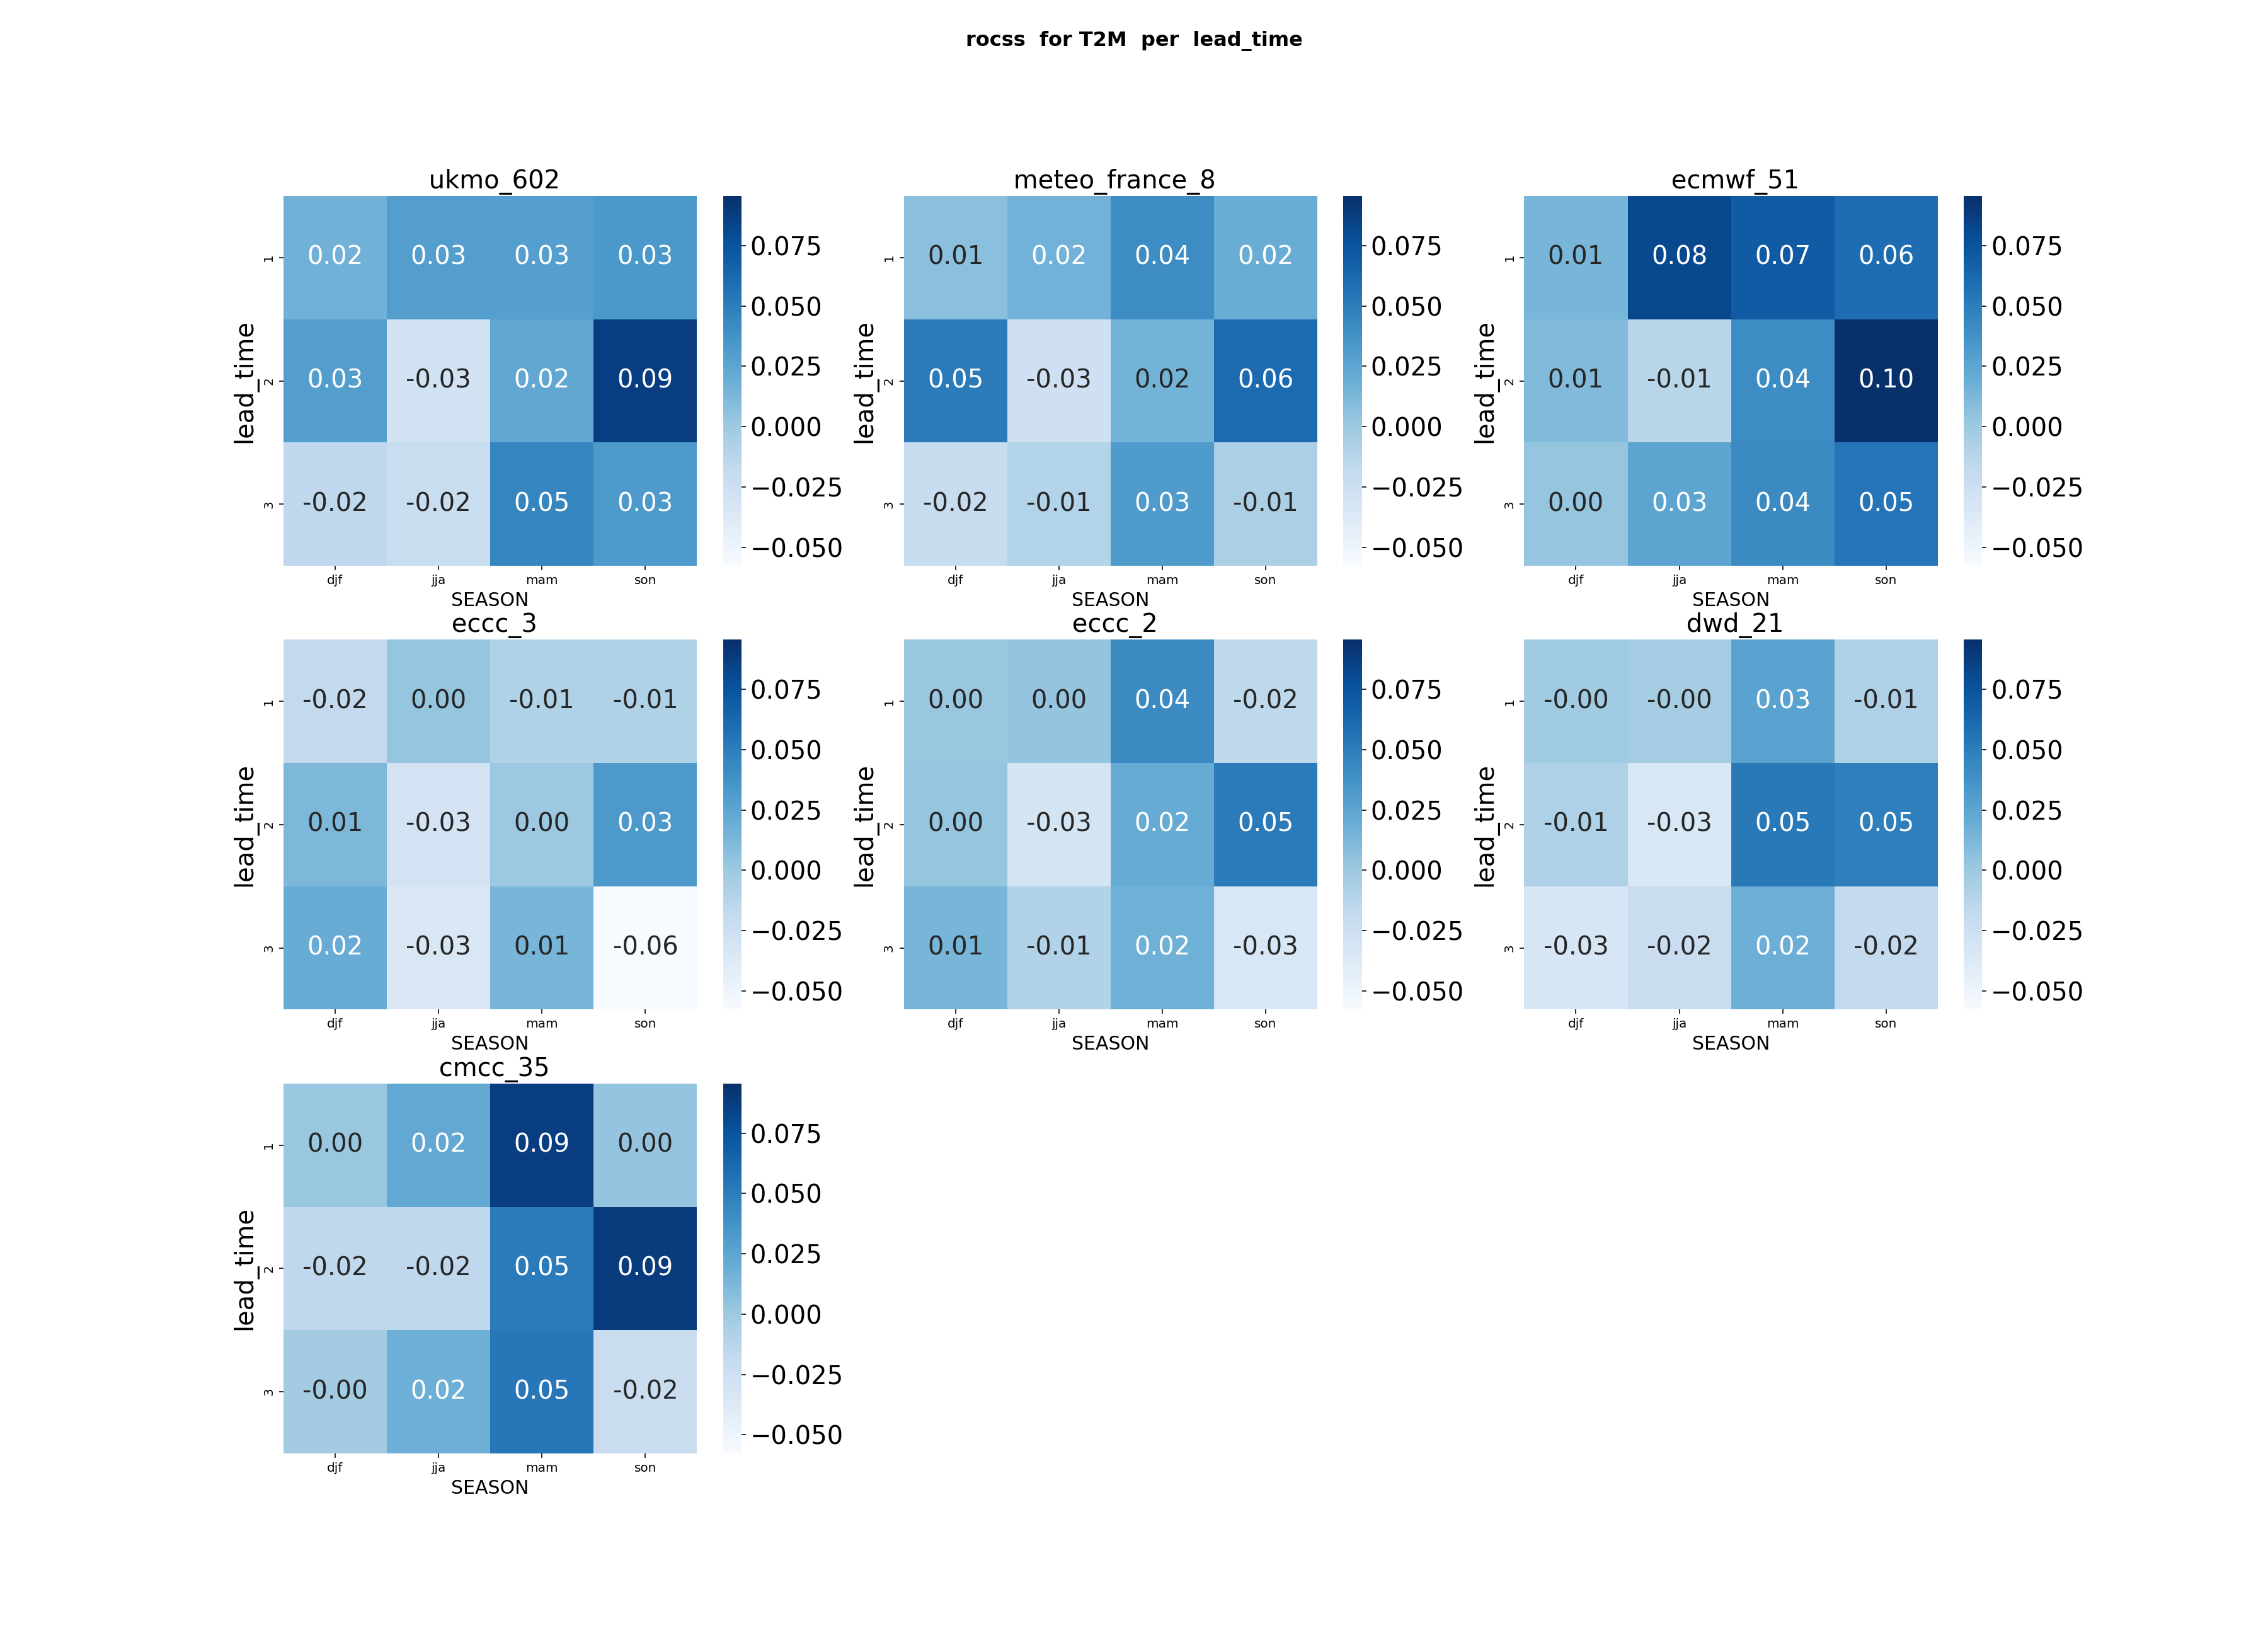
\includegraphics[width=1\linewidth]{plots/prob/rocss/rocss_T2M_lead_time.png}
    \caption{Temperature ROCSS  heatmaps for MENA region per lead-time. \textbf{\textit{(1 means perfect ROCSS)}} }
\end{figure}

The SON maintain its good performance for the second lead-time with 0.10 for the \textbf{\textit{ECMWF}} and 0.09 for the \textbf{\textit{UKMO and CMCC-35}} , in general the performance is low for all centers. The DJF and JJA exhibit the lowest performance for all centers, although, the \textbf{\textit{ECMWF}} shows relatively good performance for the 1st lead-time of JJA  (0.08).

\begin{figure}[H]
    \centering
    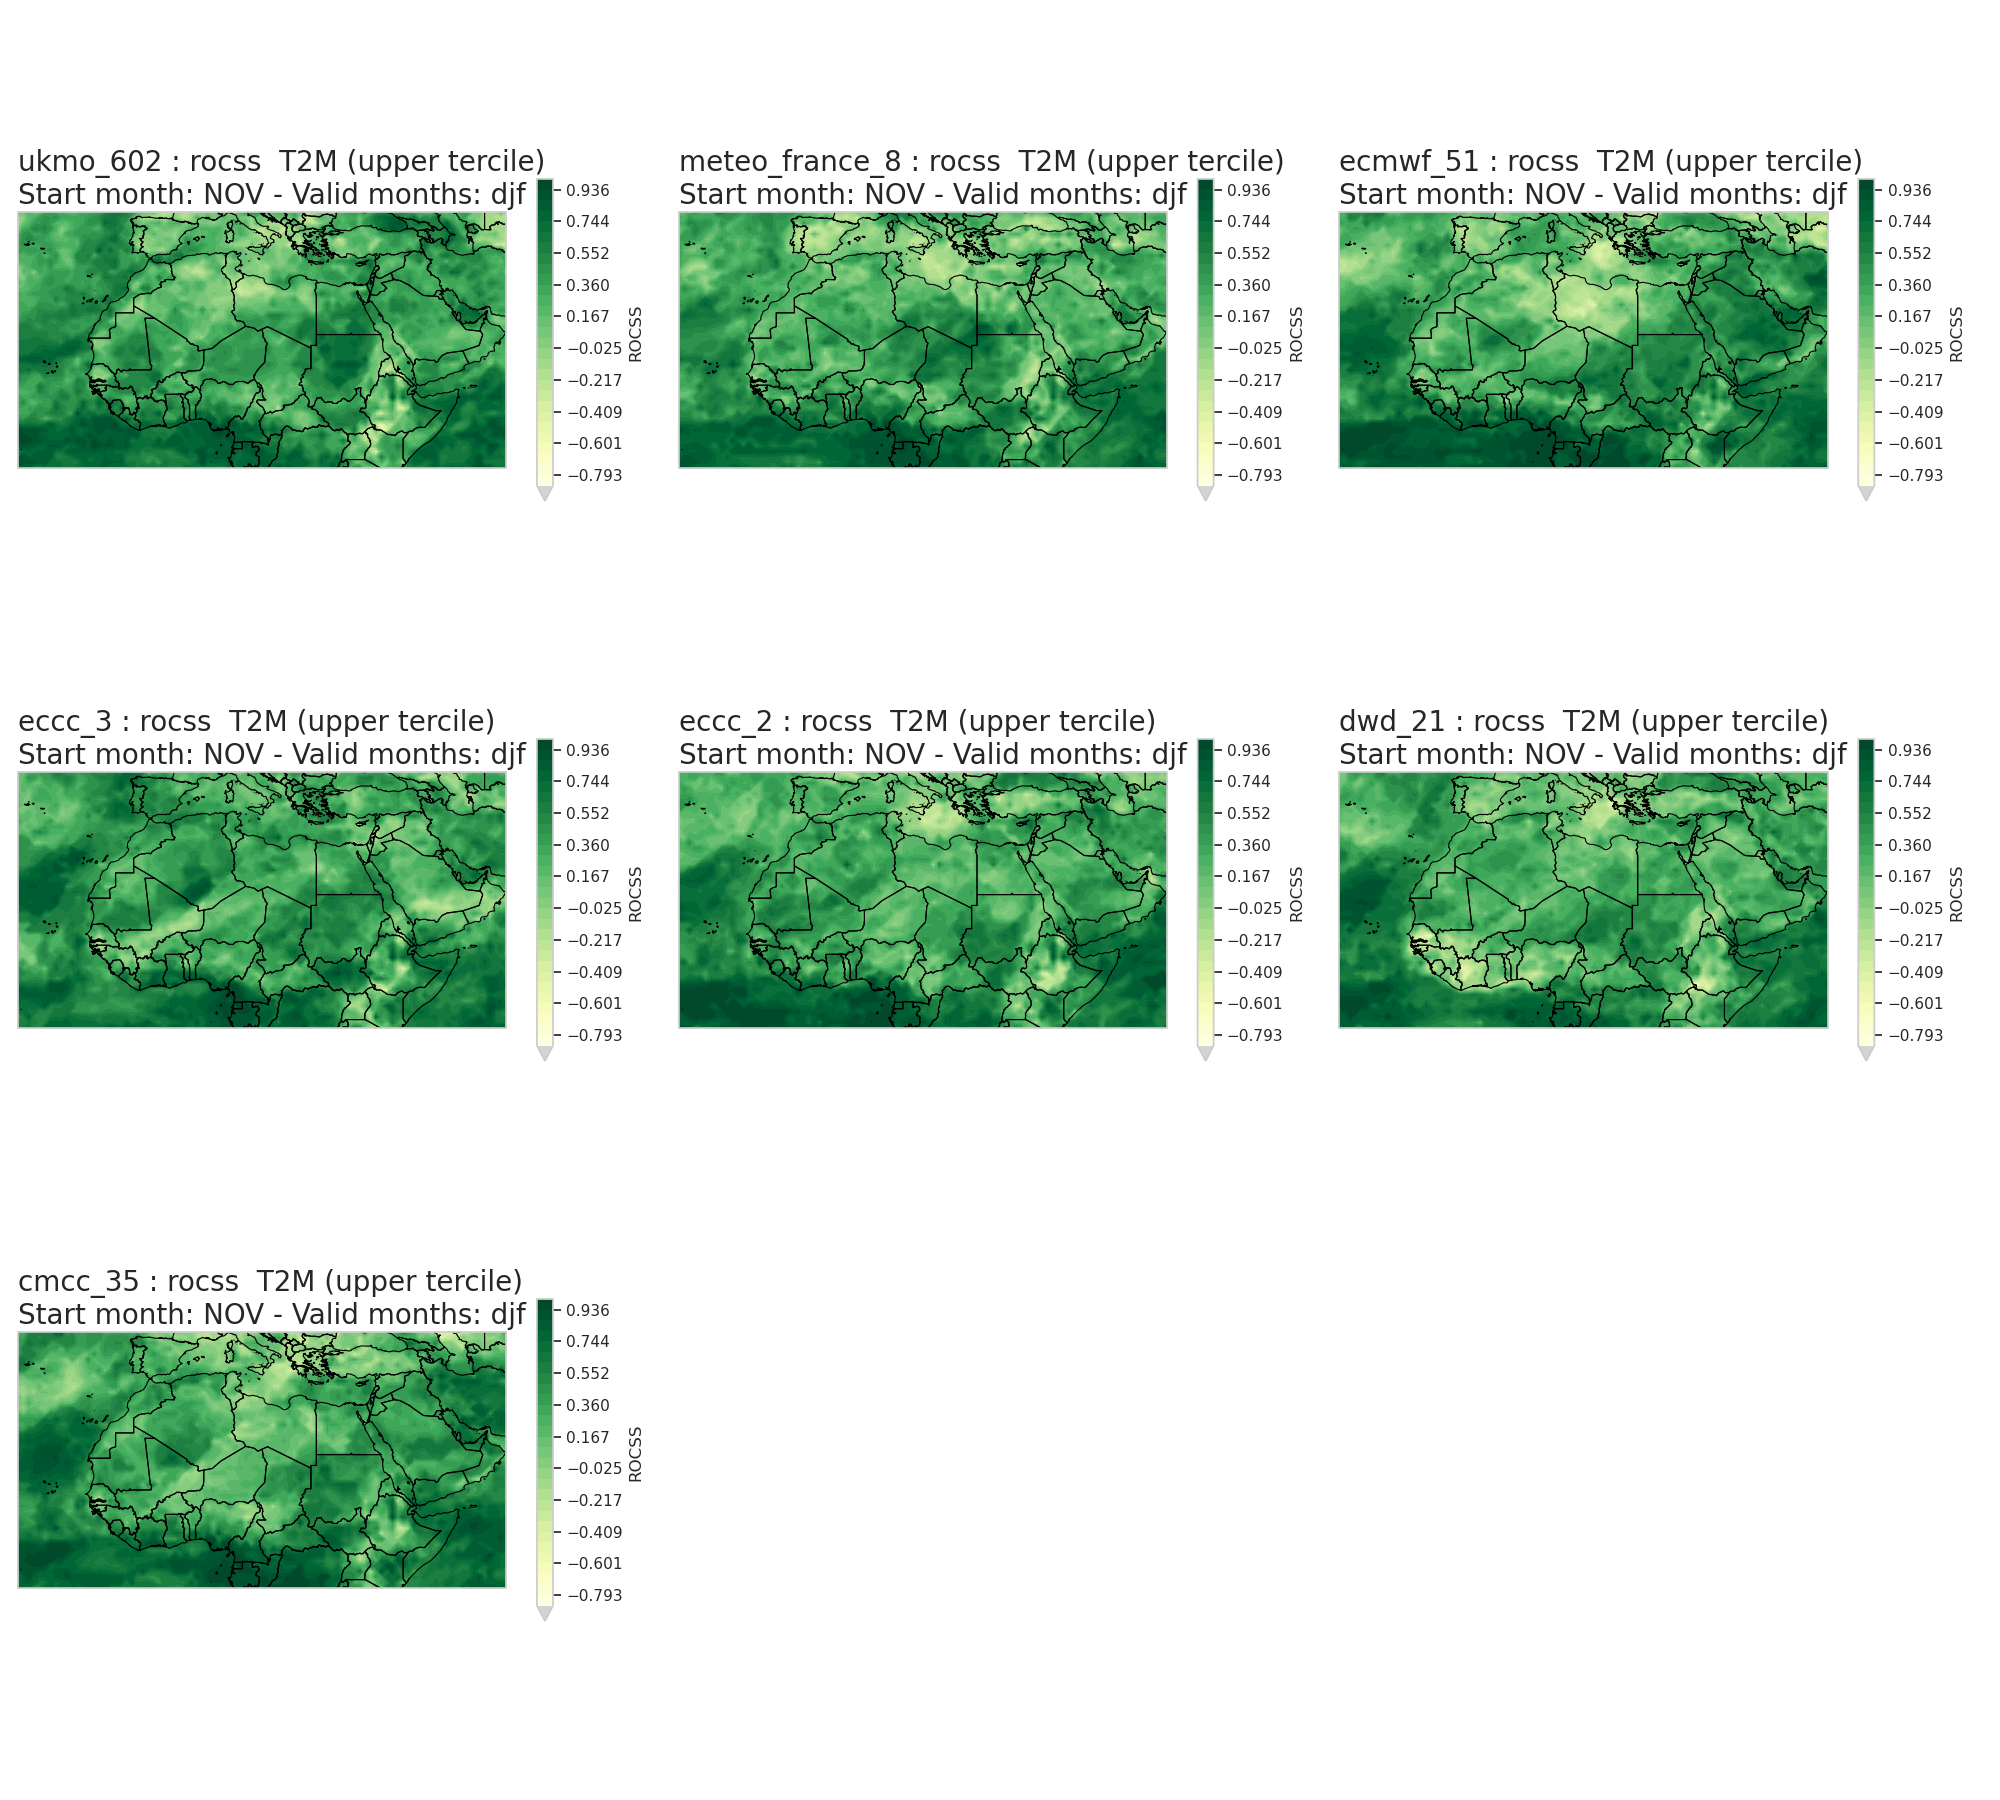
\includegraphics[width=1\linewidth]{plots/prob/rocss/rocss_djf_t2m_upper.png}
    \caption{2-meter Temperature ROCSS DJF Upper tercile \textbf{\textit{(1 means perfect ROCSS)}}}
\end{figure}

For the upper tercile of DJF, the performance is good in the equator and the Arabian Peninsula with rocss around 0.9. Nevertheless, the North Africa shows negative values which means that the forecast performs worse than random guessing, indicating a forecast that is worse than a no-skill forecast.

\begin{figure}[H]
    \centering
    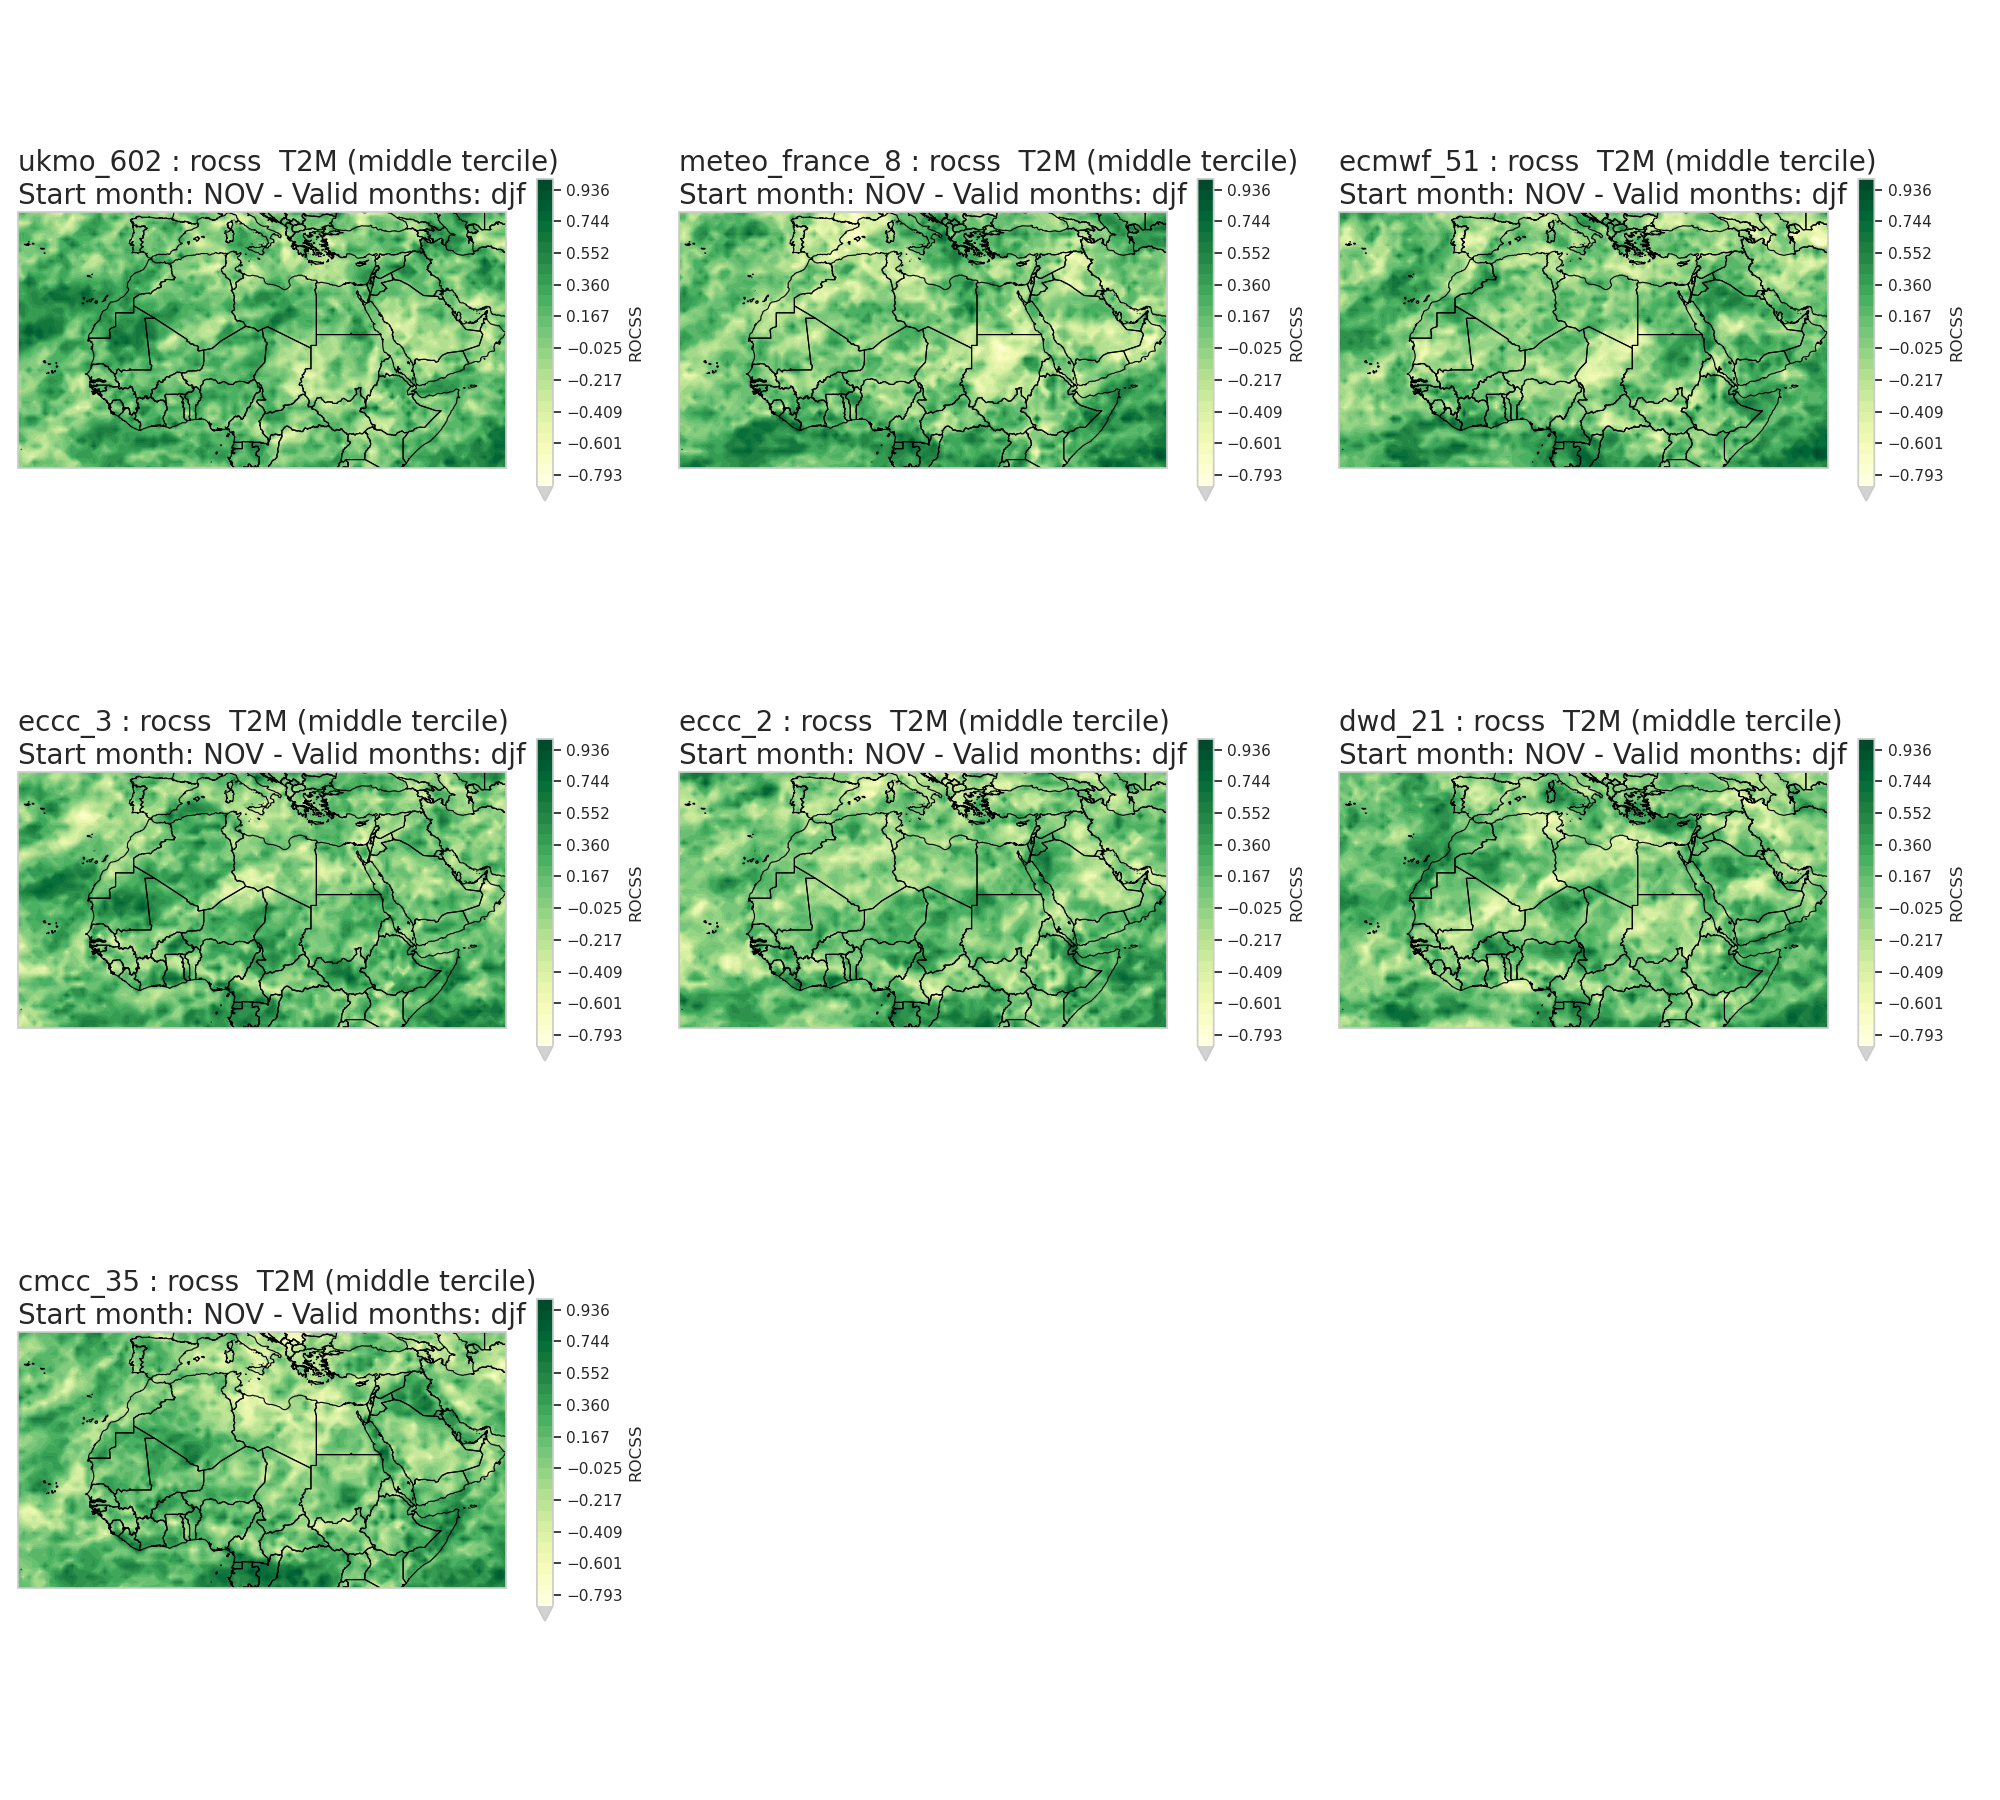
\includegraphics[width=1\linewidth]{plots/prob/rocss/rocss_djf_t2m_middle.png}
    \caption{2-meter Temperature ROCSS DJF Middle tercile \textbf{\textit{(1 means perfect ROCSS)}}}
\end{figure}

The Middle Tercile exhibits weak and inconsistent performance, with no clear spatial variability across the region. The scores are generally low and even negative in many areas, with values dropping as low as -0.79, particularly in North Africa. Despite this overall weak performance, there are a few isolated regions where the scores are notably higher, reaching up to 0.9 in certain areas of the Arabian Peninsula and along the equator. These localized high scores contrast with the broader pattern of poor performance, suggesting some regional variability in the model's predictive ability.
\paragraph{focus on north africa:}
The ROC Skill Score (ROCSS) analysis reveals similar conclusions to the ROC results for Mena region and north Africa. 
\begin{figure}[H]
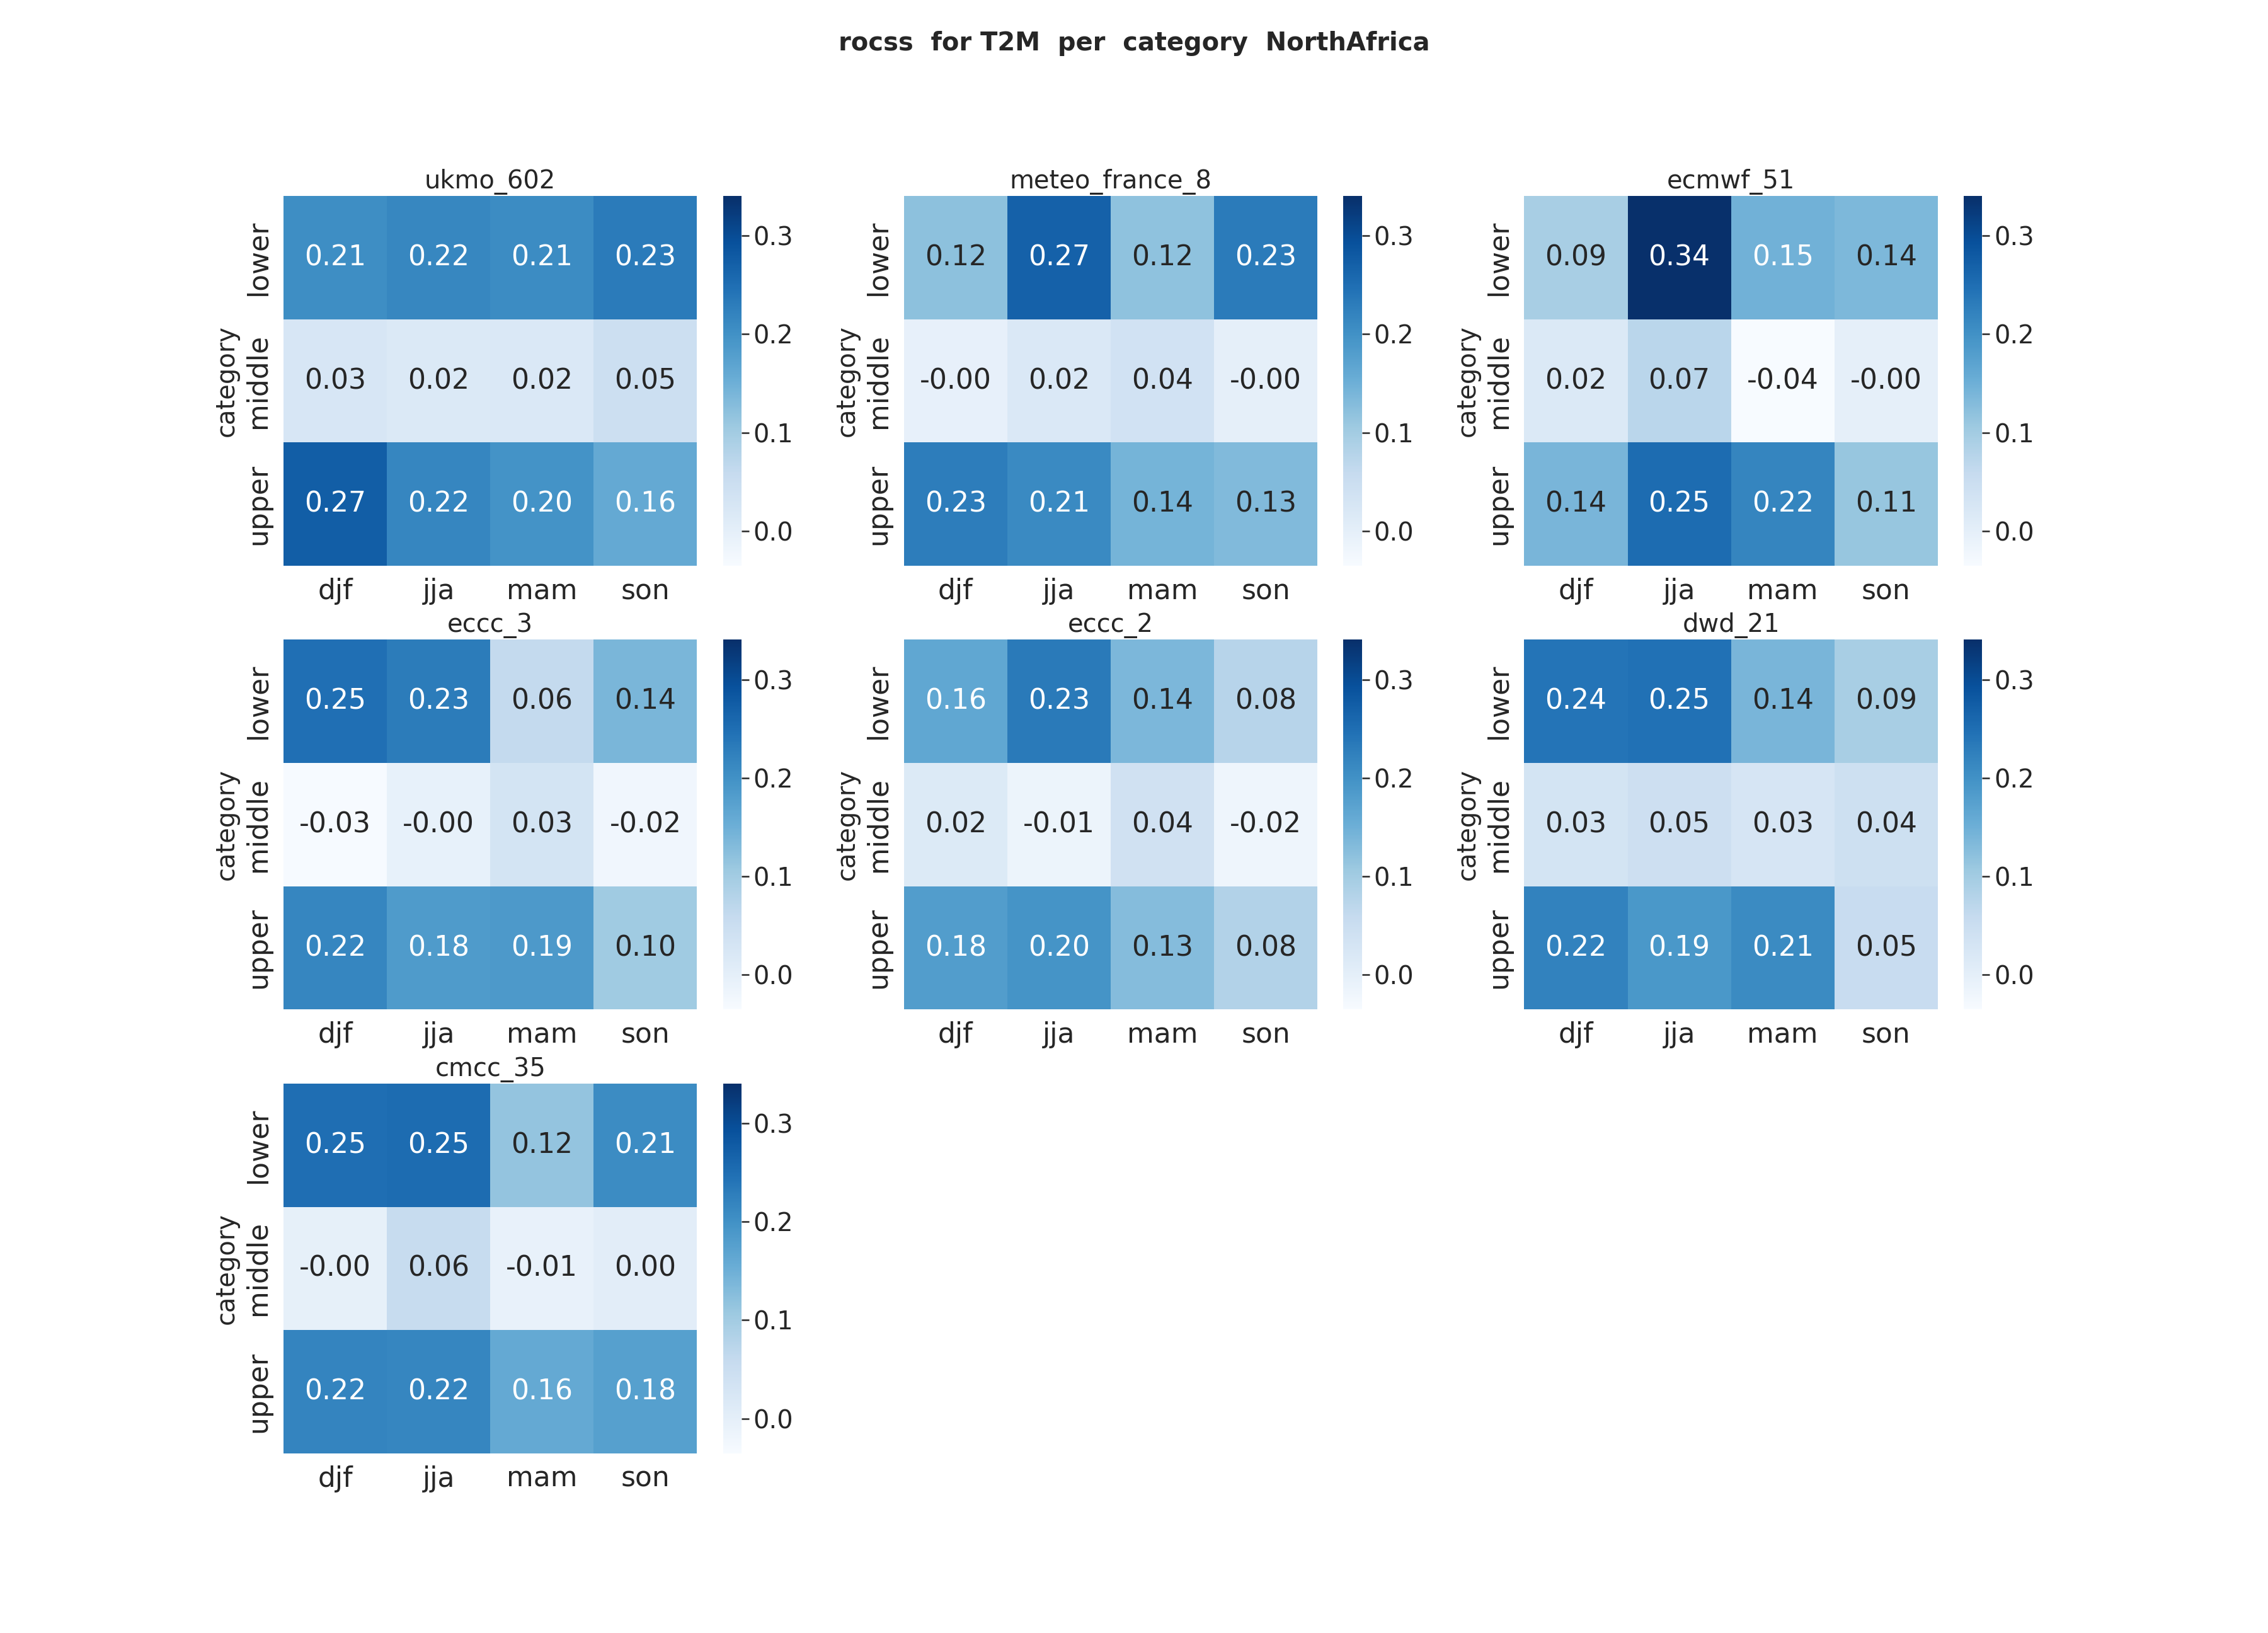
\includegraphics[scale=0.3]{plots/prob/rocss/rocss_T2M_category_NorthAfrica.png}

\caption{Temperature ROCSS  heatmaps for north africa }
\end{figure}

\paragraph{focus on Arabian Peninsula}:
There are no significant differences

\section{PRECIPITATIONS}
IN general, the forecast of precipitations is more complicated than temperature, thus the scores are a little less good for this part especially the deterministic ones. 
\subsection{Deterministic Evaluation Metrics}

\subsubsection{Anomaly Correlation Coefficient}

\begin{figure}[H]
	\centering
	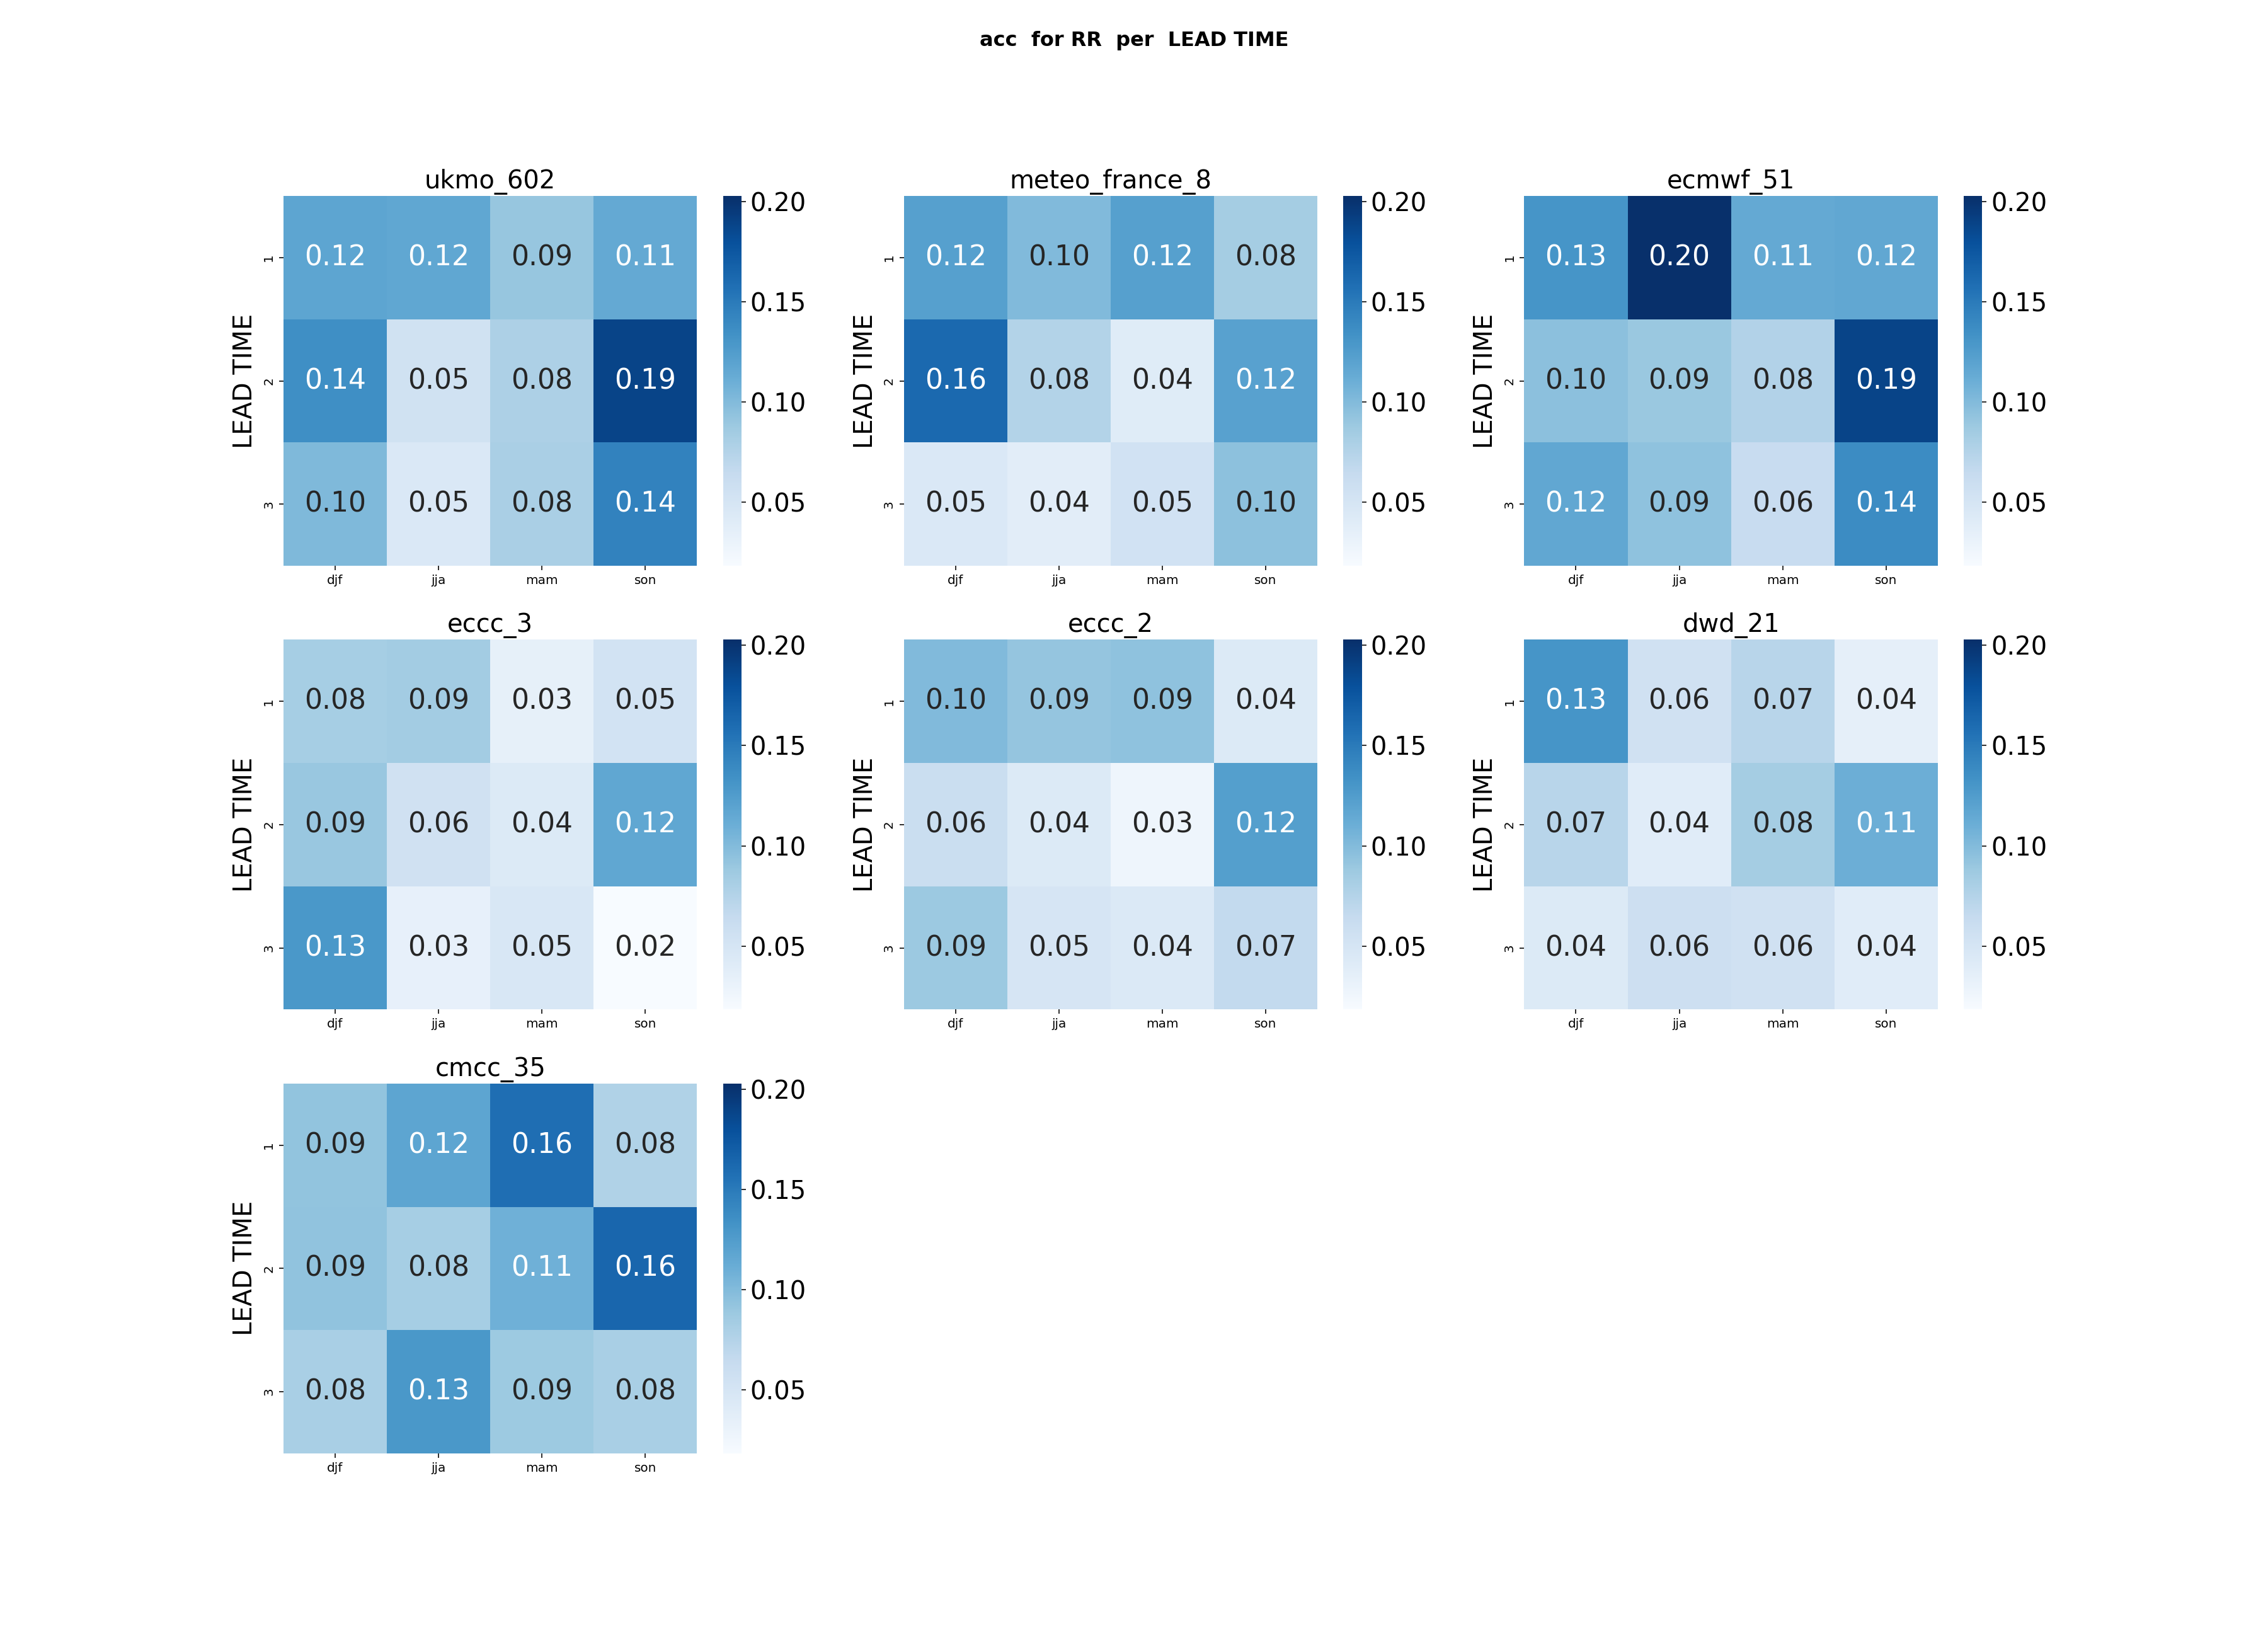
\includegraphics[scale=0.25]{plots/det/acc/acc_RR_mena.png}
	\caption{The Heatmap of acc for the mena region for every period \textbf{\textit{(1 for perfect ACC)} }}
\end{figure}
The acc is moderate for all centers; however, the best models are \textbf{\textit{ECMWF, UKMO, and CMCC-35}}. There is no clear variability in performance along lead-time. For SON, the performance is good at lead-time 2 for all centers. As for the other seasons, the performance is generally strong at the 1st lead-time but decreases with increasing lead-time.
Hence, Meteo-France also shows good performance, but it decreases significantly over time.



\begin{figure}[H]
\centering
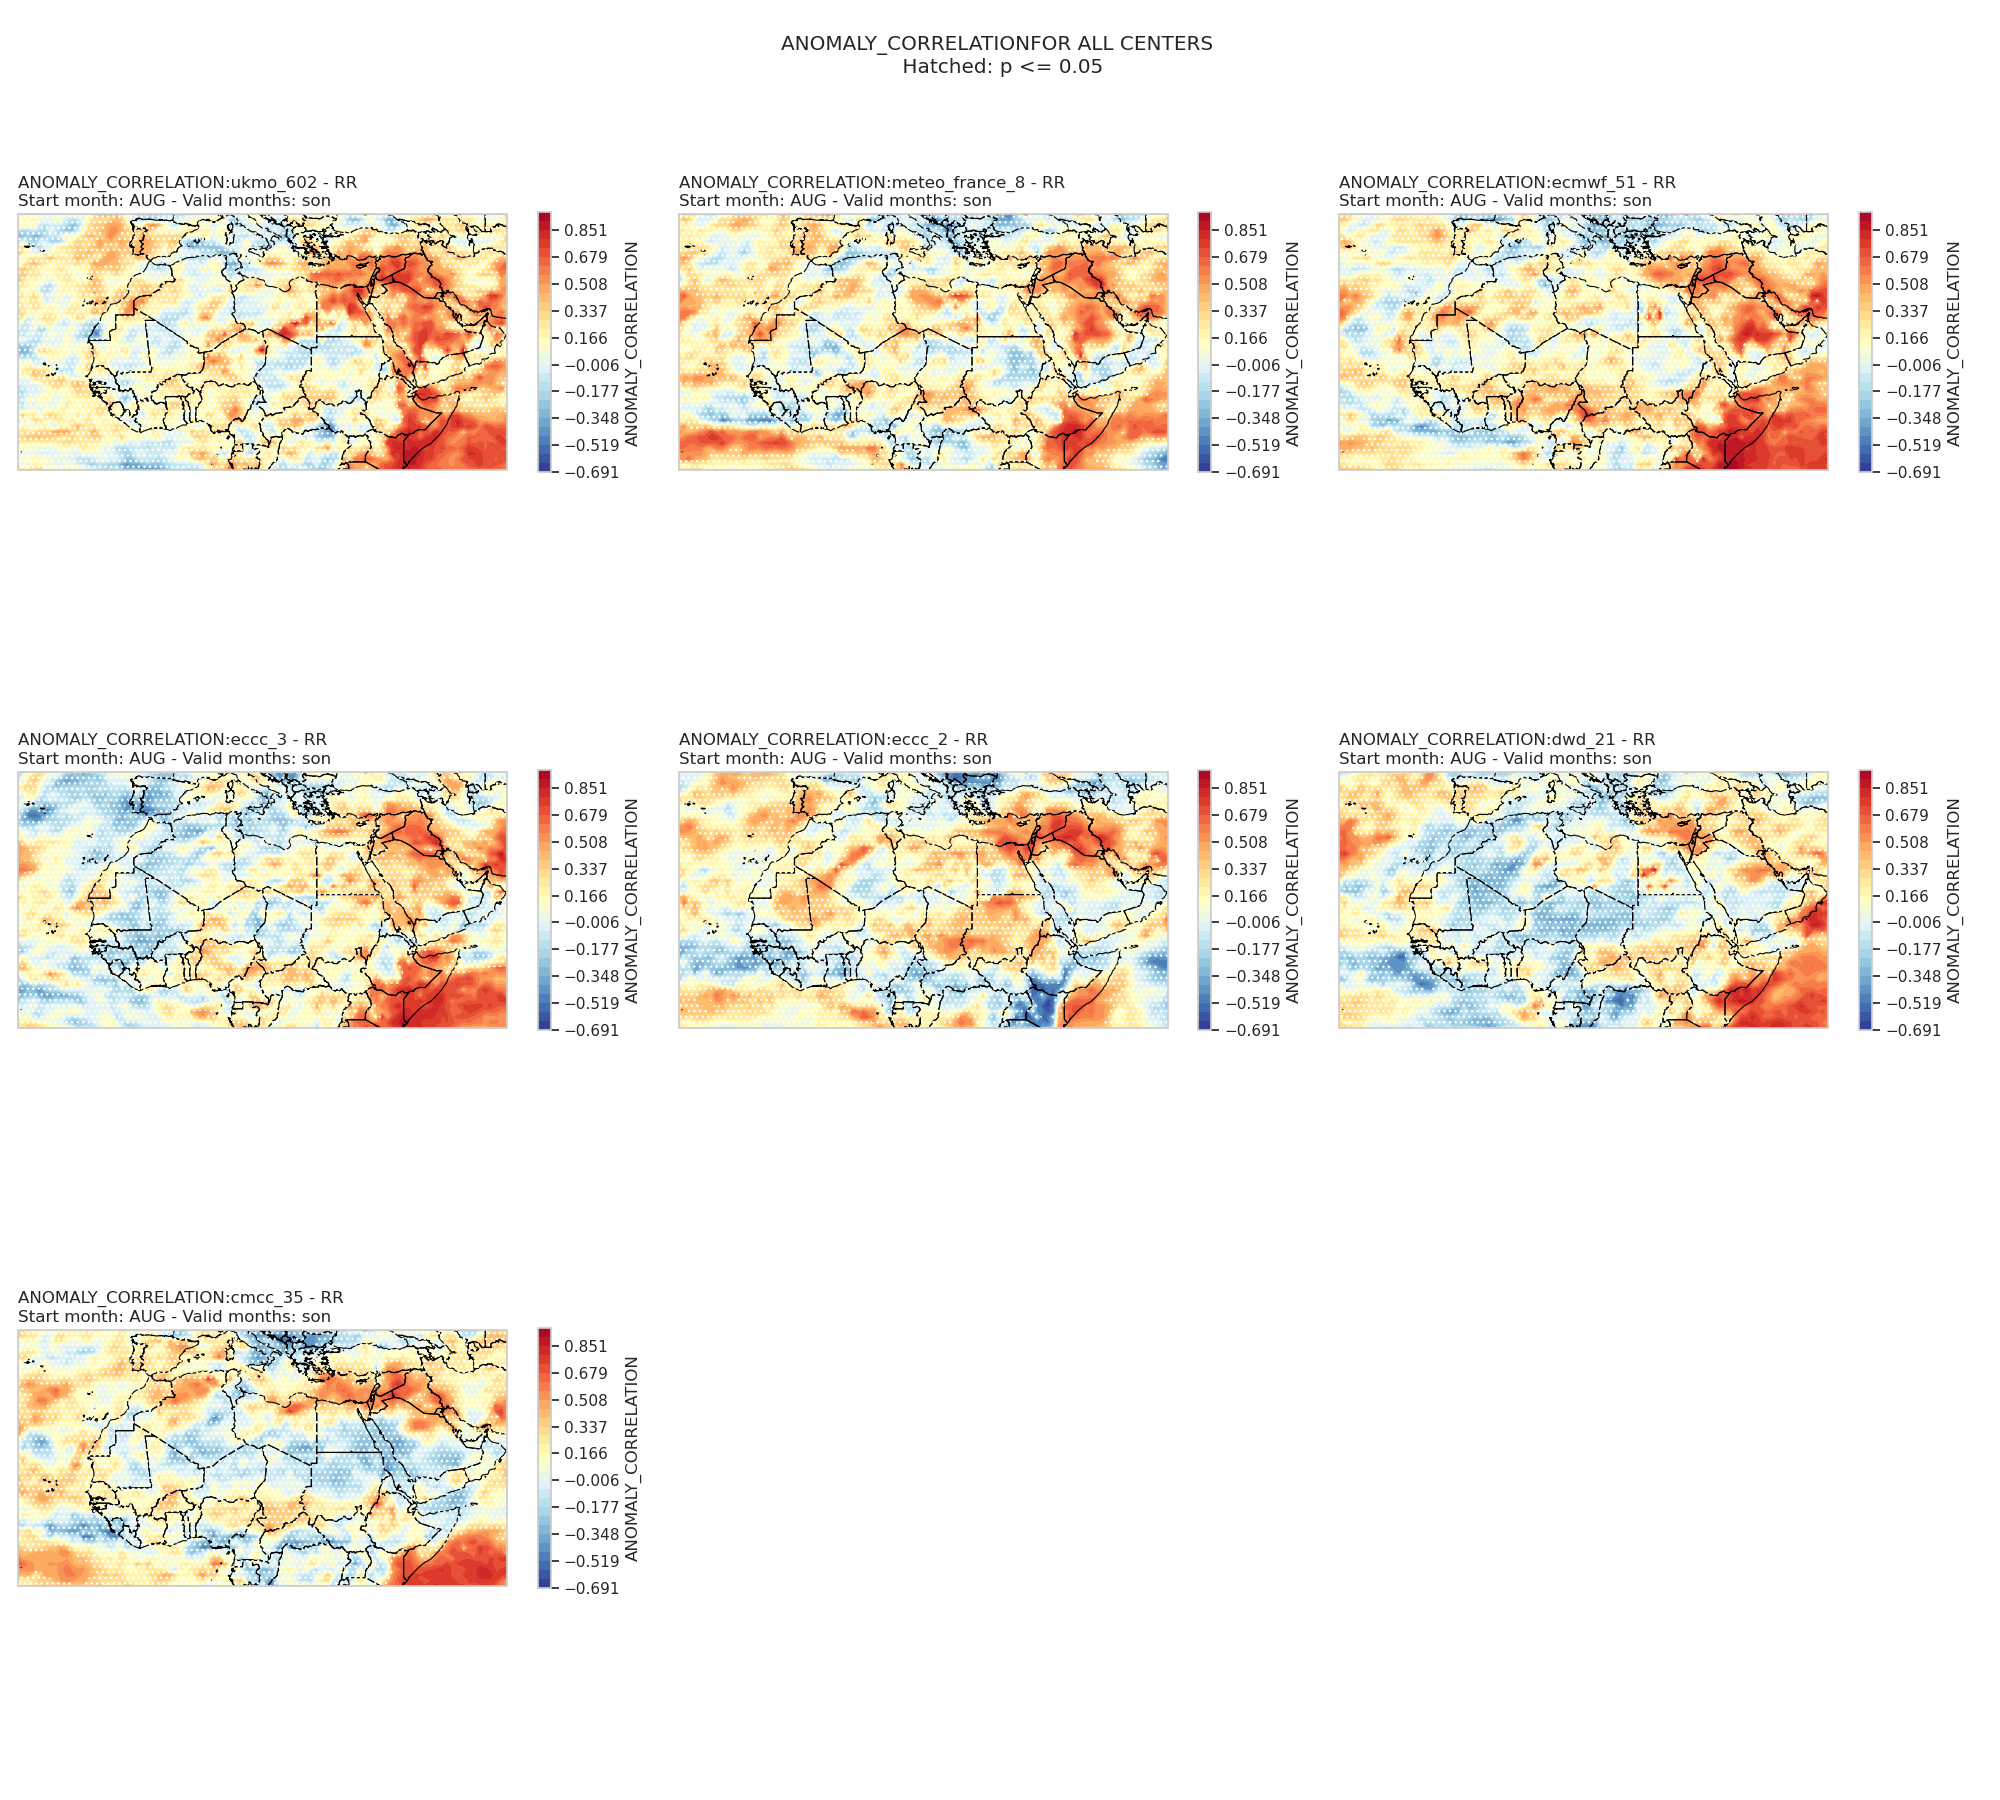
\includegraphics[scale=0.3]{plots/det/acc/ANOMALY_CORRELATION_son_RR.png}
\caption{3-months Rolling mean of Anomaly Correlation in MENA Region for all centers SON}
\end{figure}
For temperature, the models demonstrate the best performance in the tropical regions. However, for precipitation, the situation is different. Hence the results show good performance during SON, where the Arabian Peninsula and  East Africa exhibit the highest performance.
\begin{figure}[H]
\centering
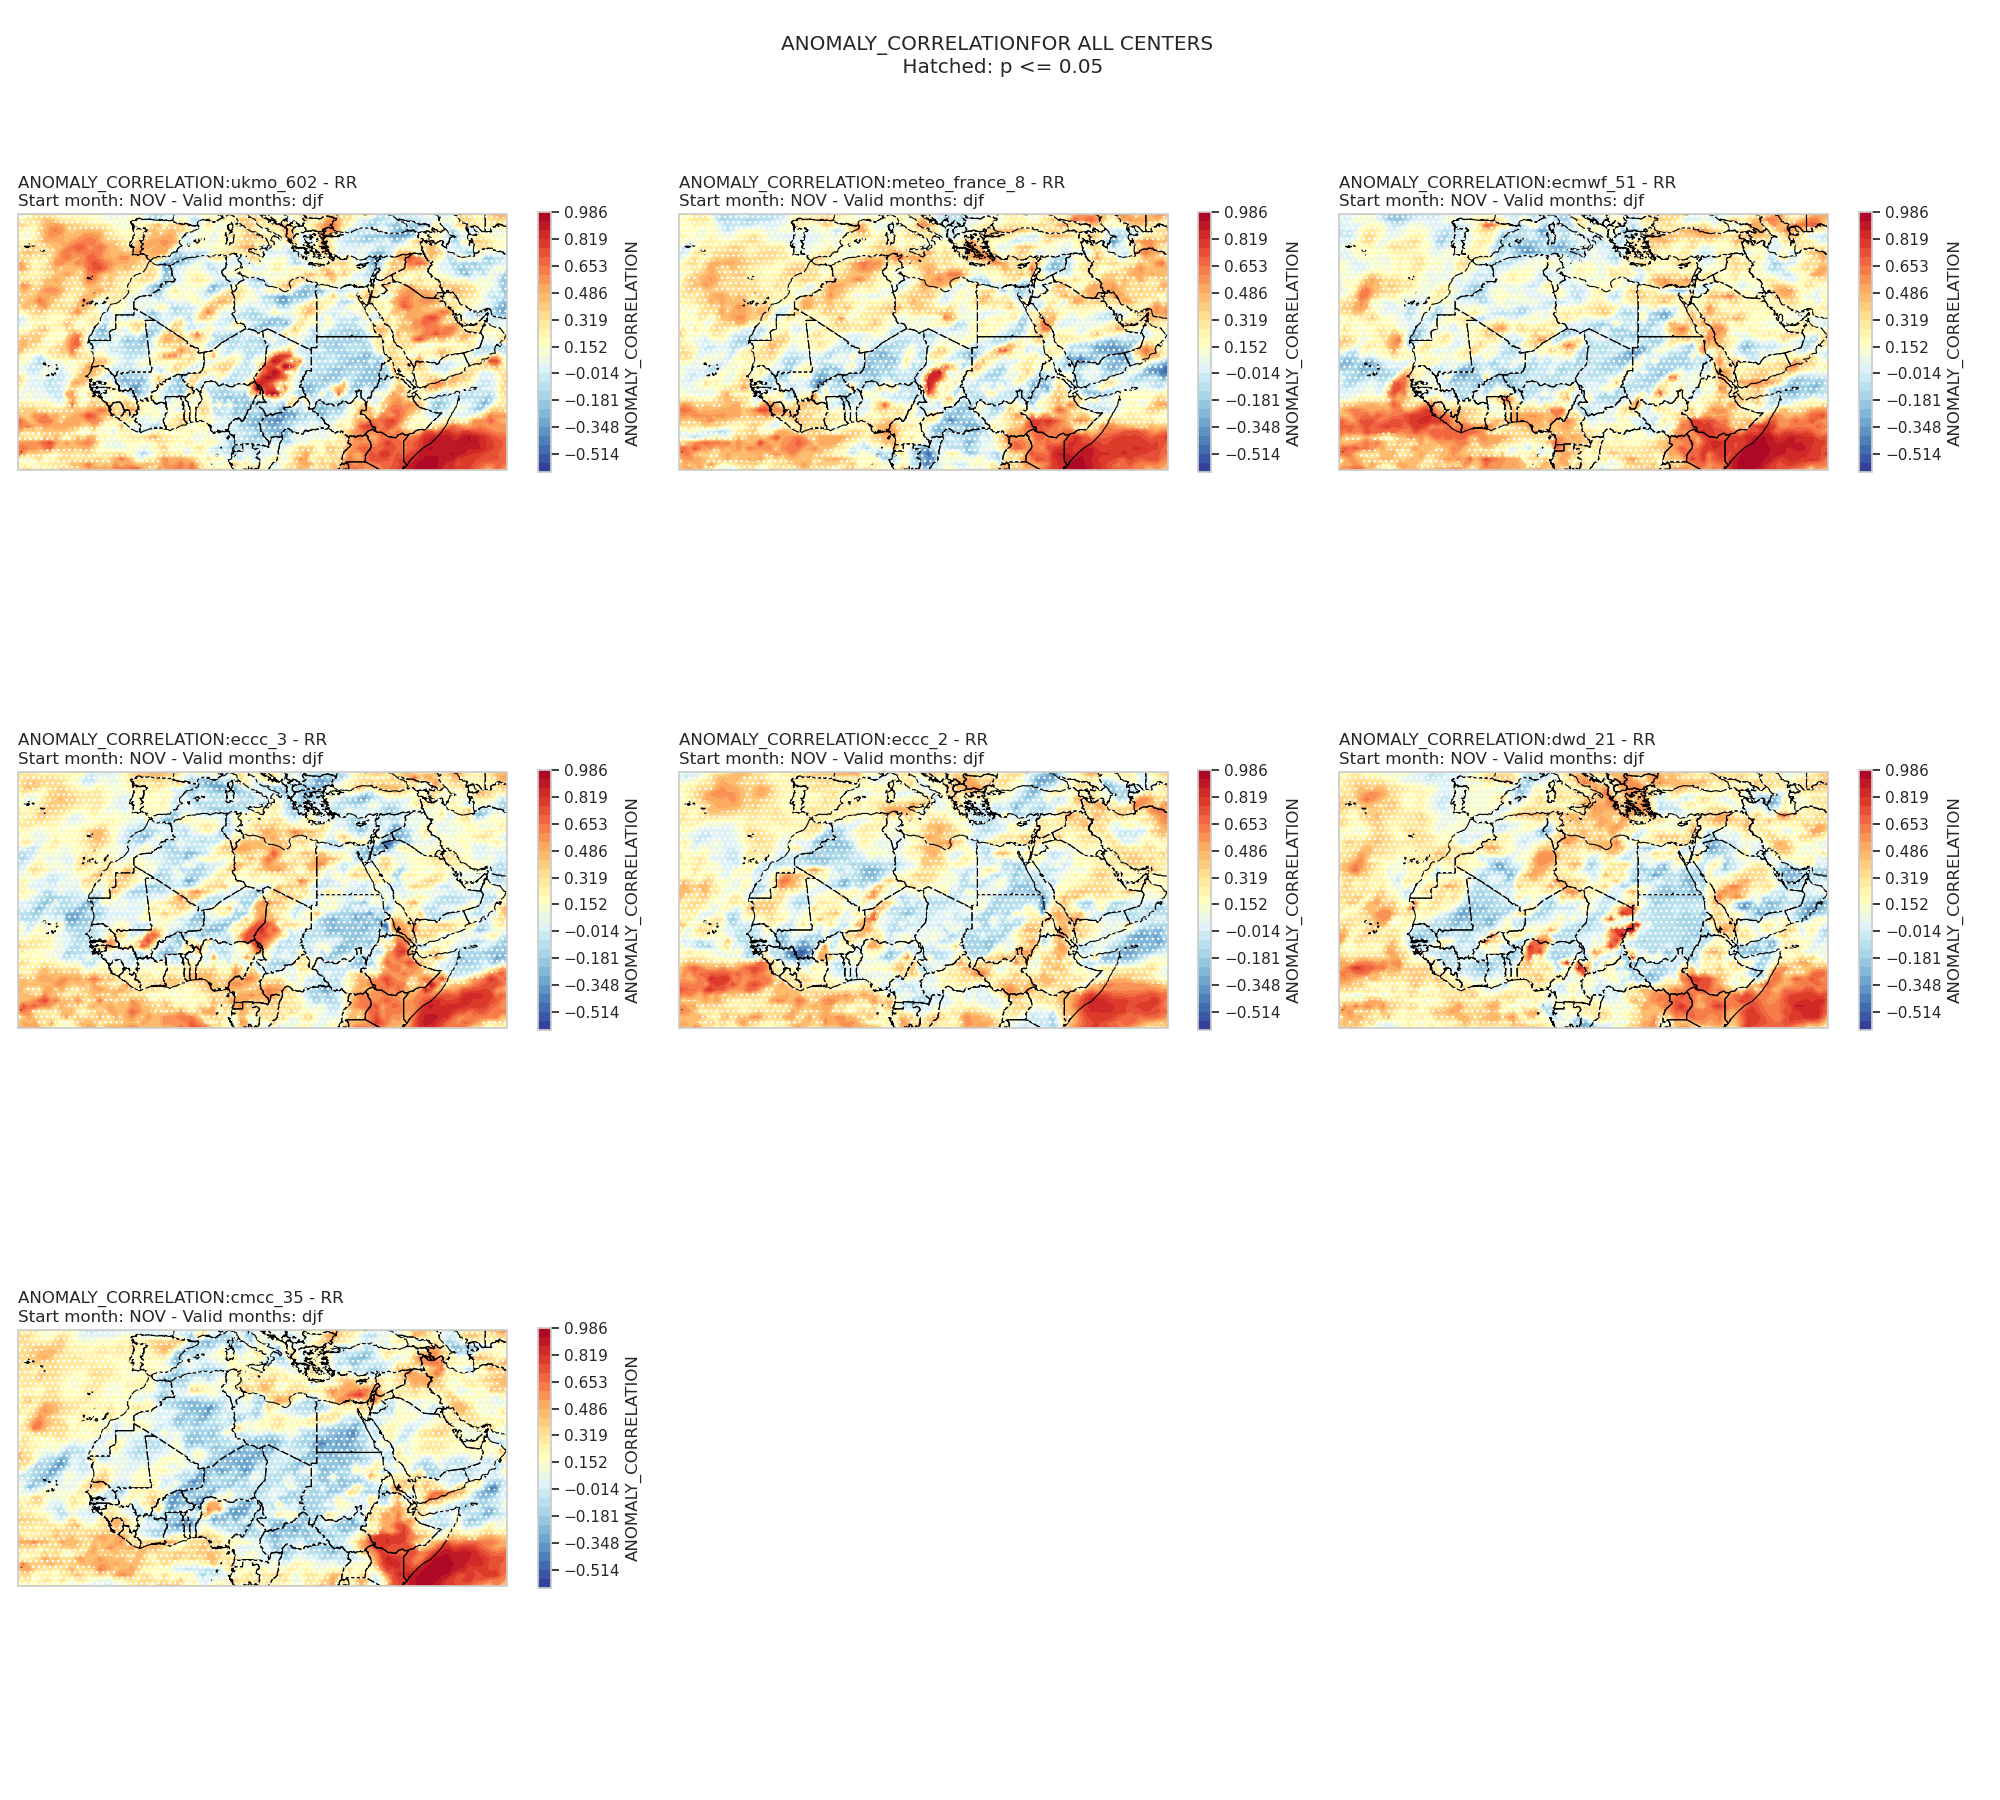
\includegraphics[scale=0.3]{plots/det/acc/ANOMALY_CORRELATION_djf_RR.png}
\caption{3-months Rolling mean of Anomaly Correlation in MENA Region for all centers DJF}
\end{figure}

The 3-month rolling mean for DJF acc shows that the best models are \textbf{\textit{ECMWF, UKMO, and Meteo-France}}. The acc is significant across most of the MENA region, except in the east of Africa. Thus, for all centers the East of Africa have the highest score. However, the \textbf{\textit{ecmwf and ukmo}} show good performance for 


 
For SON, the situation is generally better than for DJF in the Arabian peninsula. In general, \textbf{\textit{ECMWF and Meteo-France}} are the best. Nevertheless, the ACC isn't significant in the east of africa and the north of the Arabian peninsula despite of the high acc.


\paragraph{focus on north africa:}
according to the heatmap below, the correlation shows no big difference for the first lead-time, but for the second and third lead-times, it became lower. Thus, the \textbf{\textit{ecmwf,ukmo and meteo-france}} maintain relatively good correlation.


\begin{figure}[H]
	\centering
	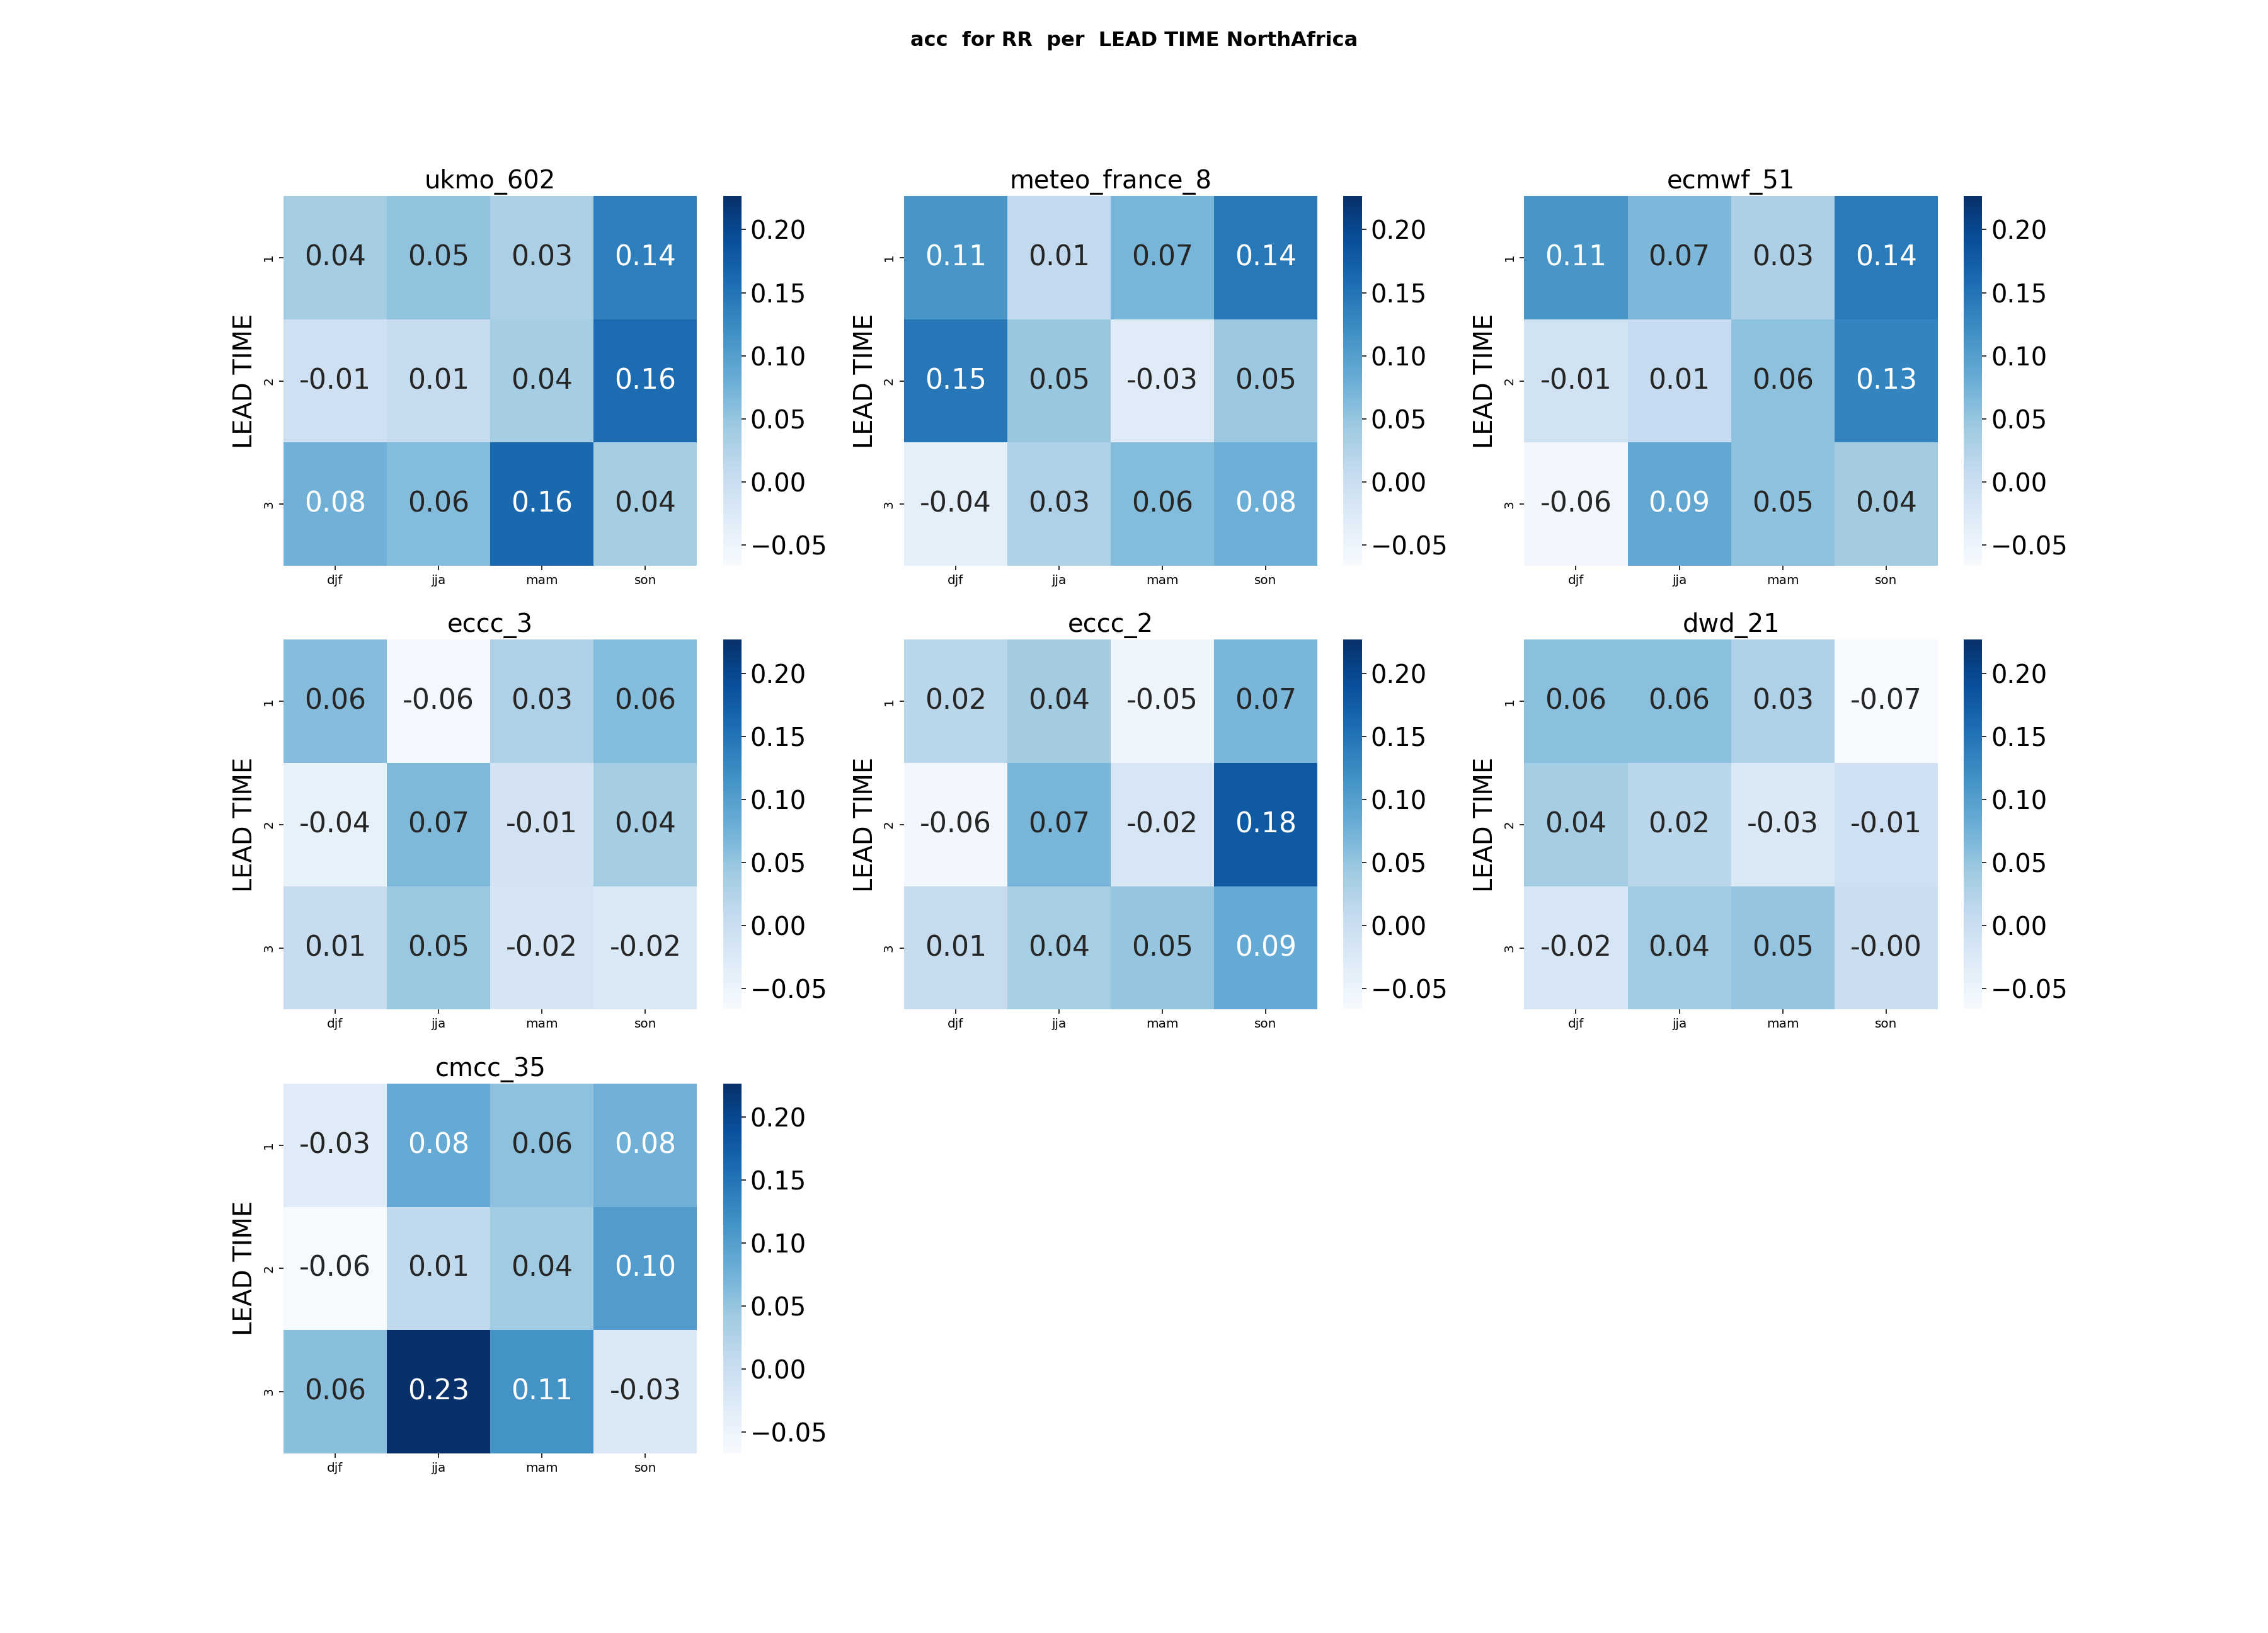
\includegraphics[scale=0.25]{plots/det/acc/acc_RR_NorthAfrica.png}
	\caption{The Heatmap of ACC for the North Africa region for every period \textbf{\textit{(1 for perfect Correlation)} }}
\end{figure}

\vspace{1.5cm}
\paragraph{focus on Arabian Peninsula}:

\begin{figure}[H]
	\centering
	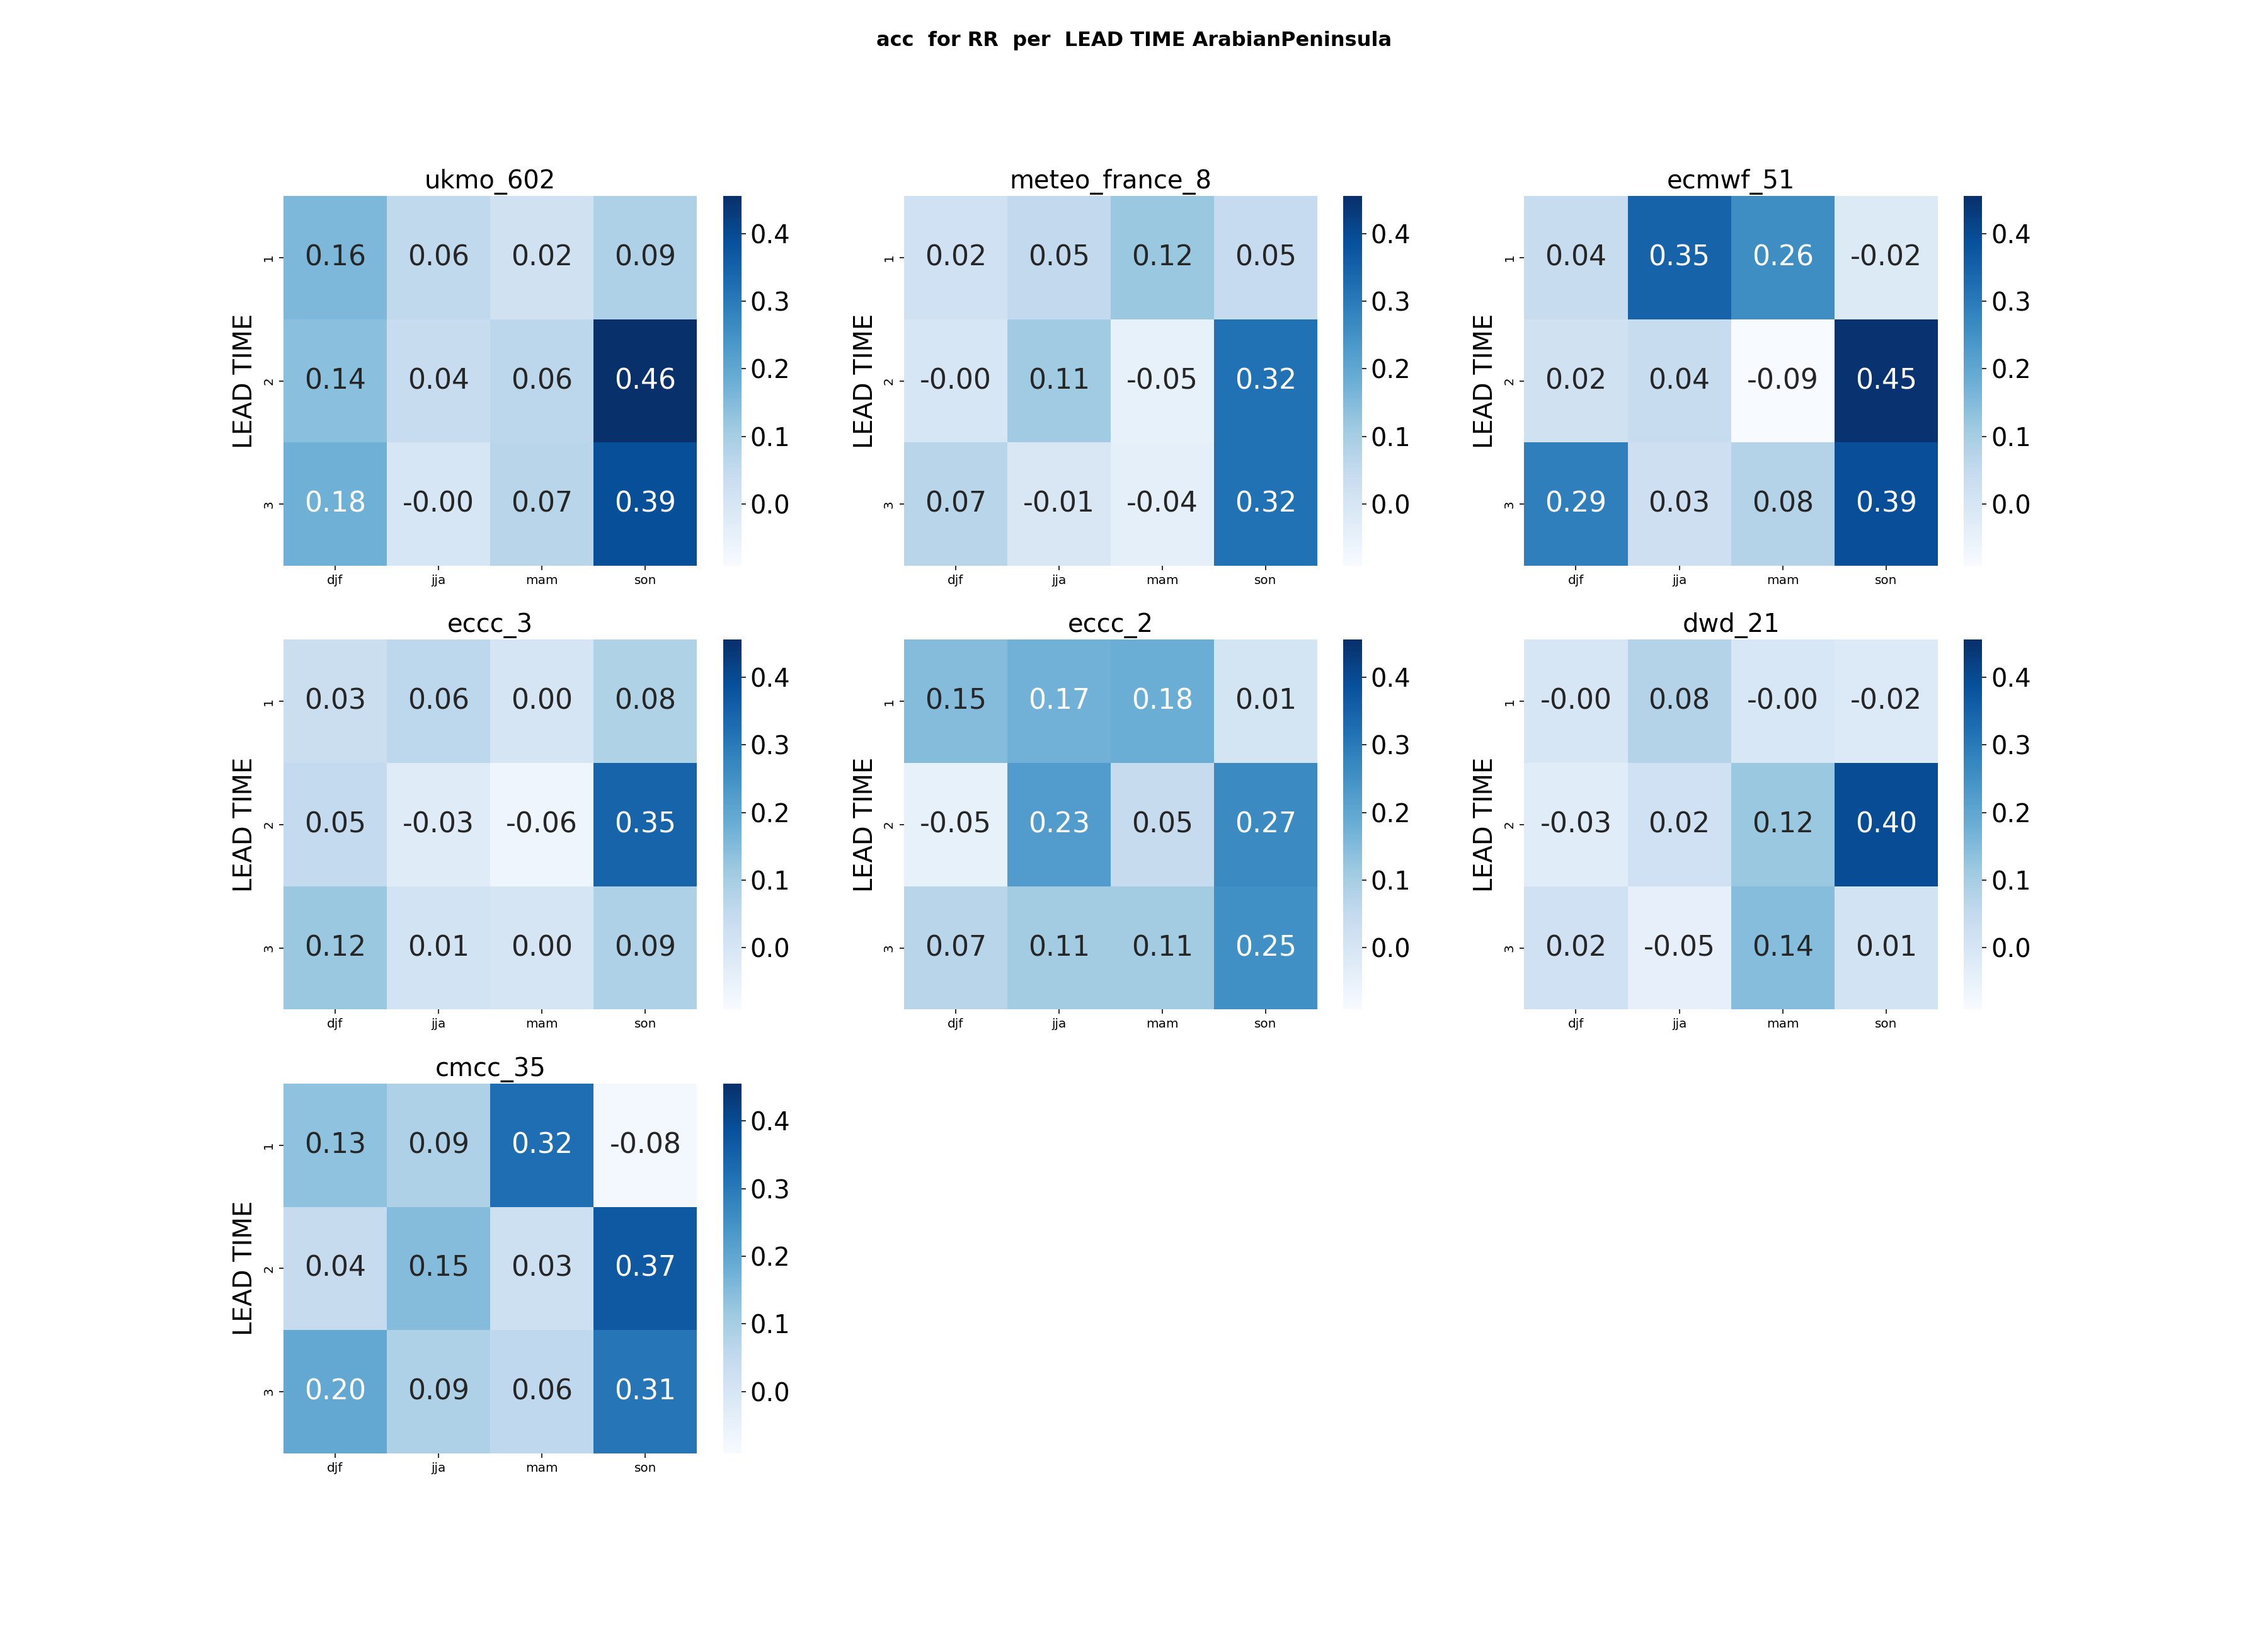
\includegraphics[scale=0.25]{plots/det/acc/acc_RR_ArabianPeninsula.png}
	\caption{The Heatmap of acc for the Arabian Peninsula region for every period  \textbf{\textit{(1 for perfect ACC)} }}
\end{figure}

The analysis of the Arabian Peninsula shows that the score is much better than the general situation of the mena region. The acc is good especially for SON for the second and third lead-times.

\subsubsection{Root Mean Square Error}
 


\begin{figure}[H]
\centering
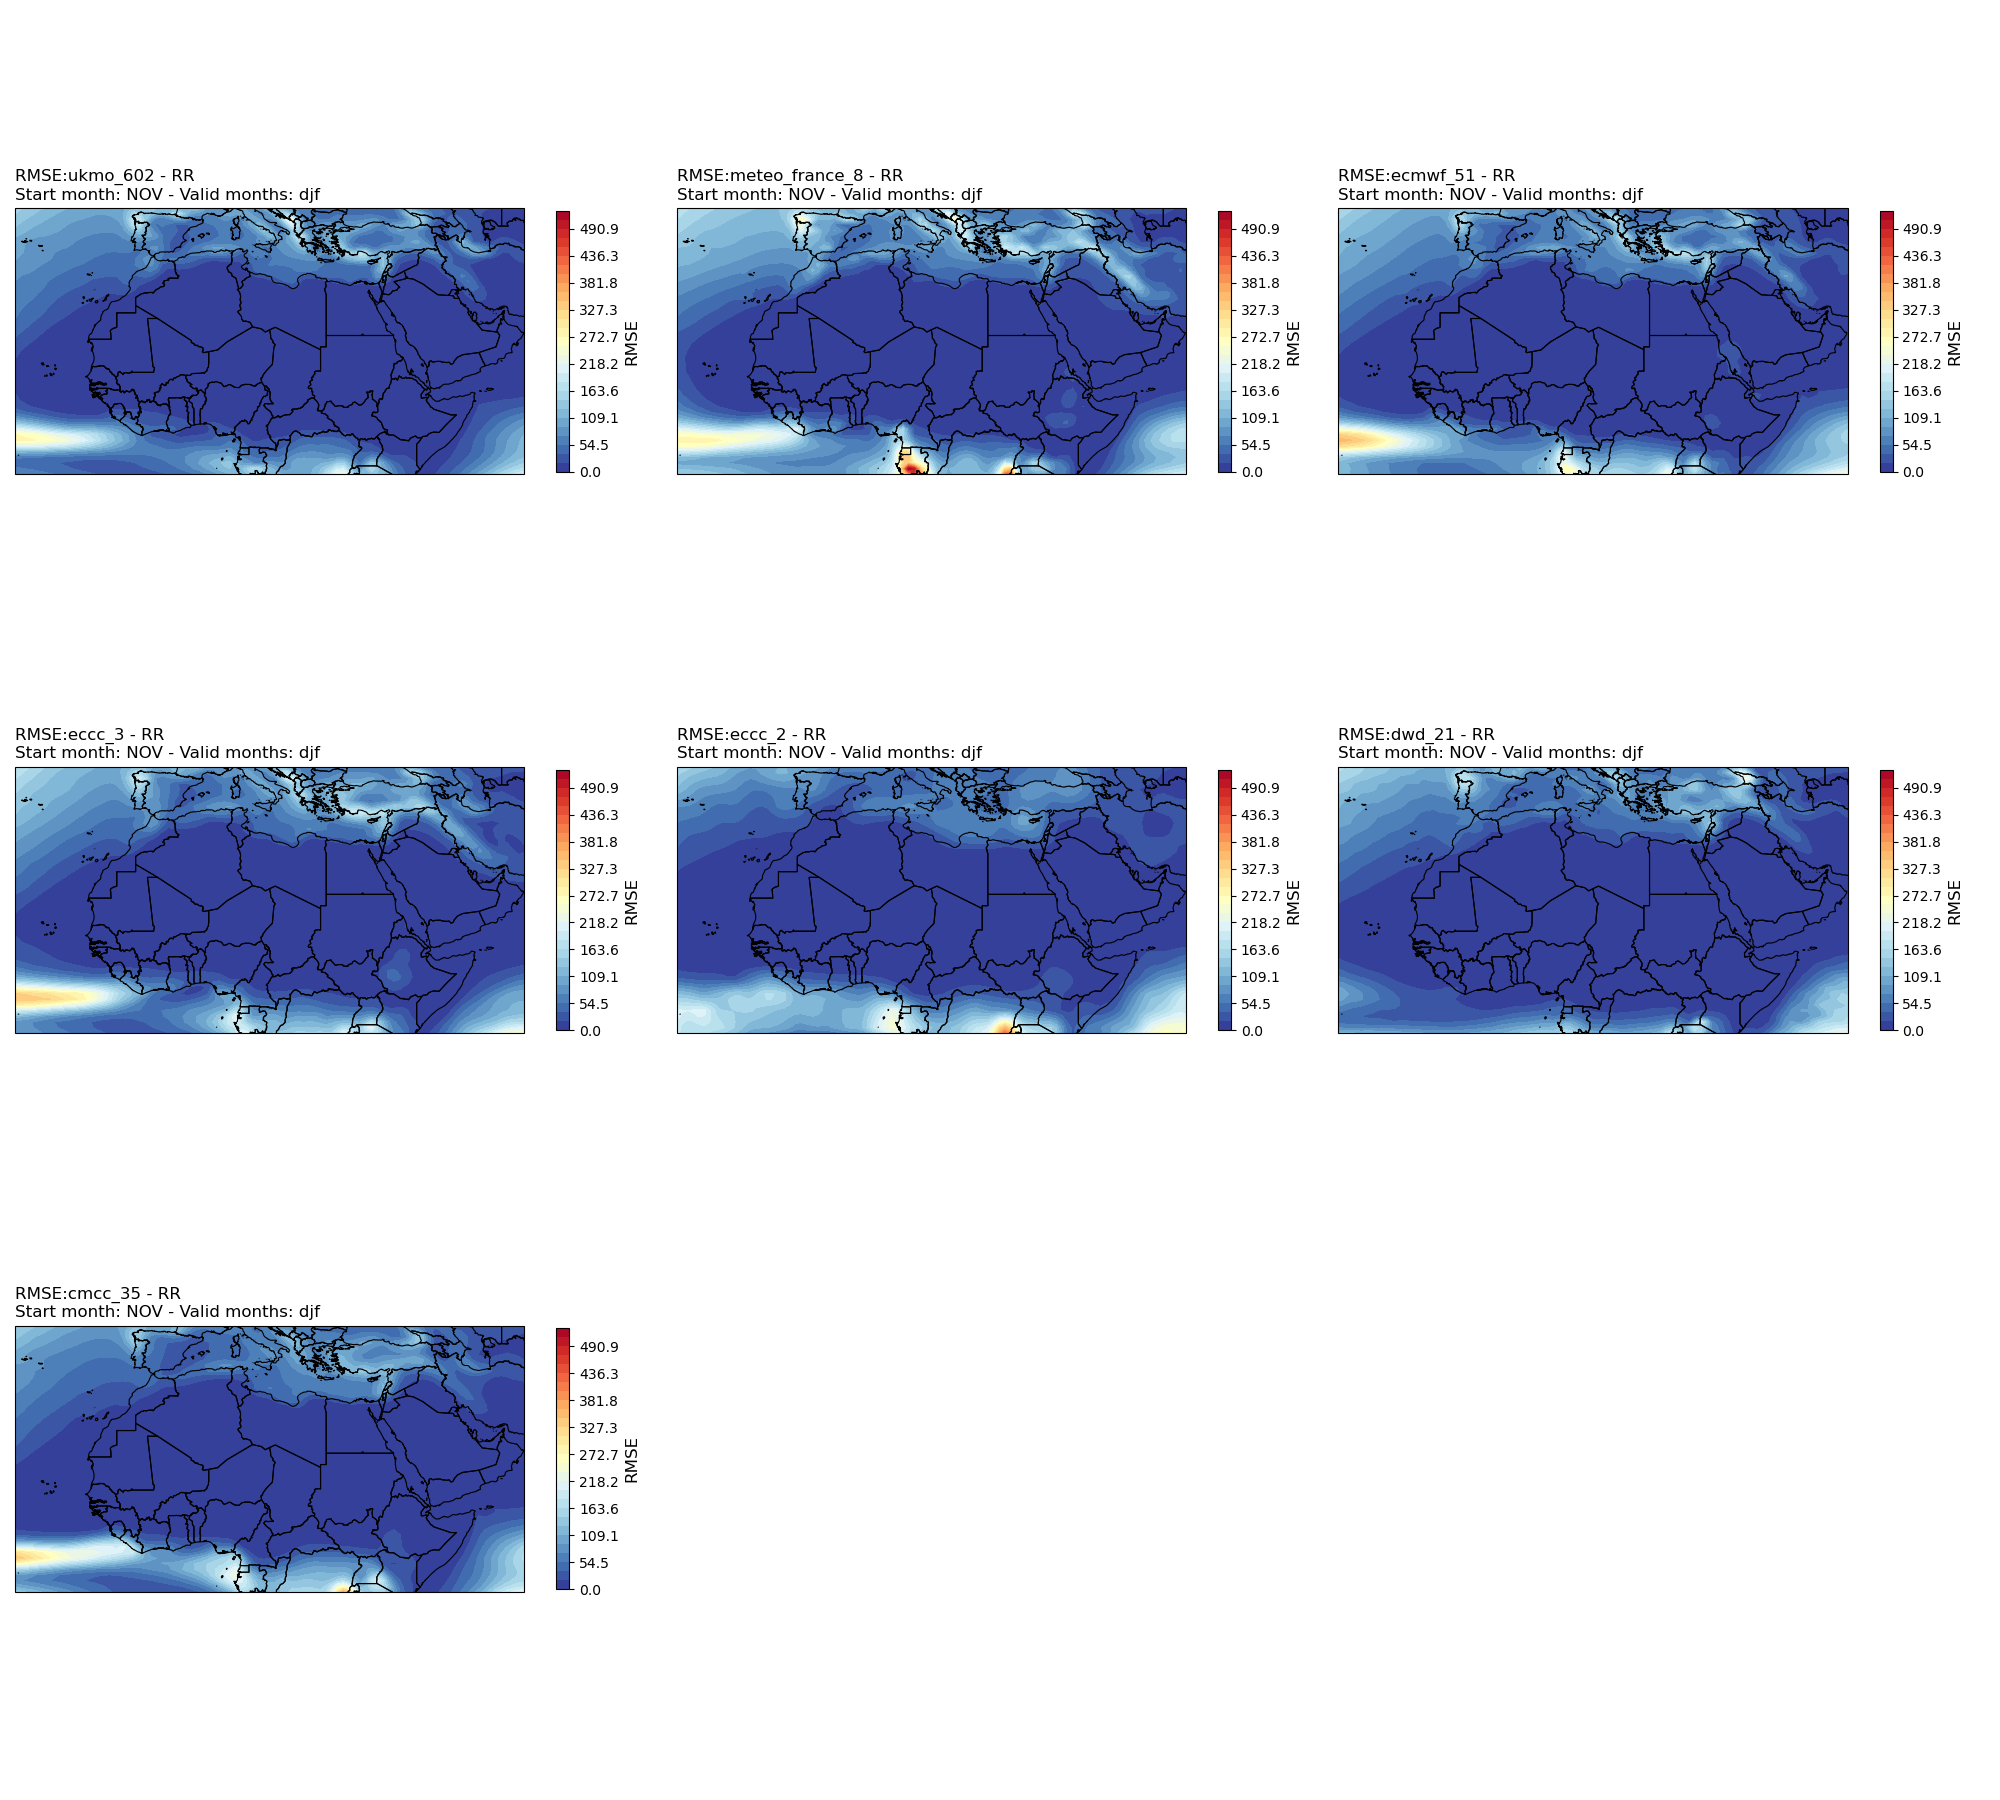
\includegraphics[scale=0.3]{plots/det/rmse/rmse_djf_RR.png}
\caption{3-months Rolling mean of RMSE in MENA Region for all centers DJF in mm}
\end{figure}

\begin{figure}[H]
\centering
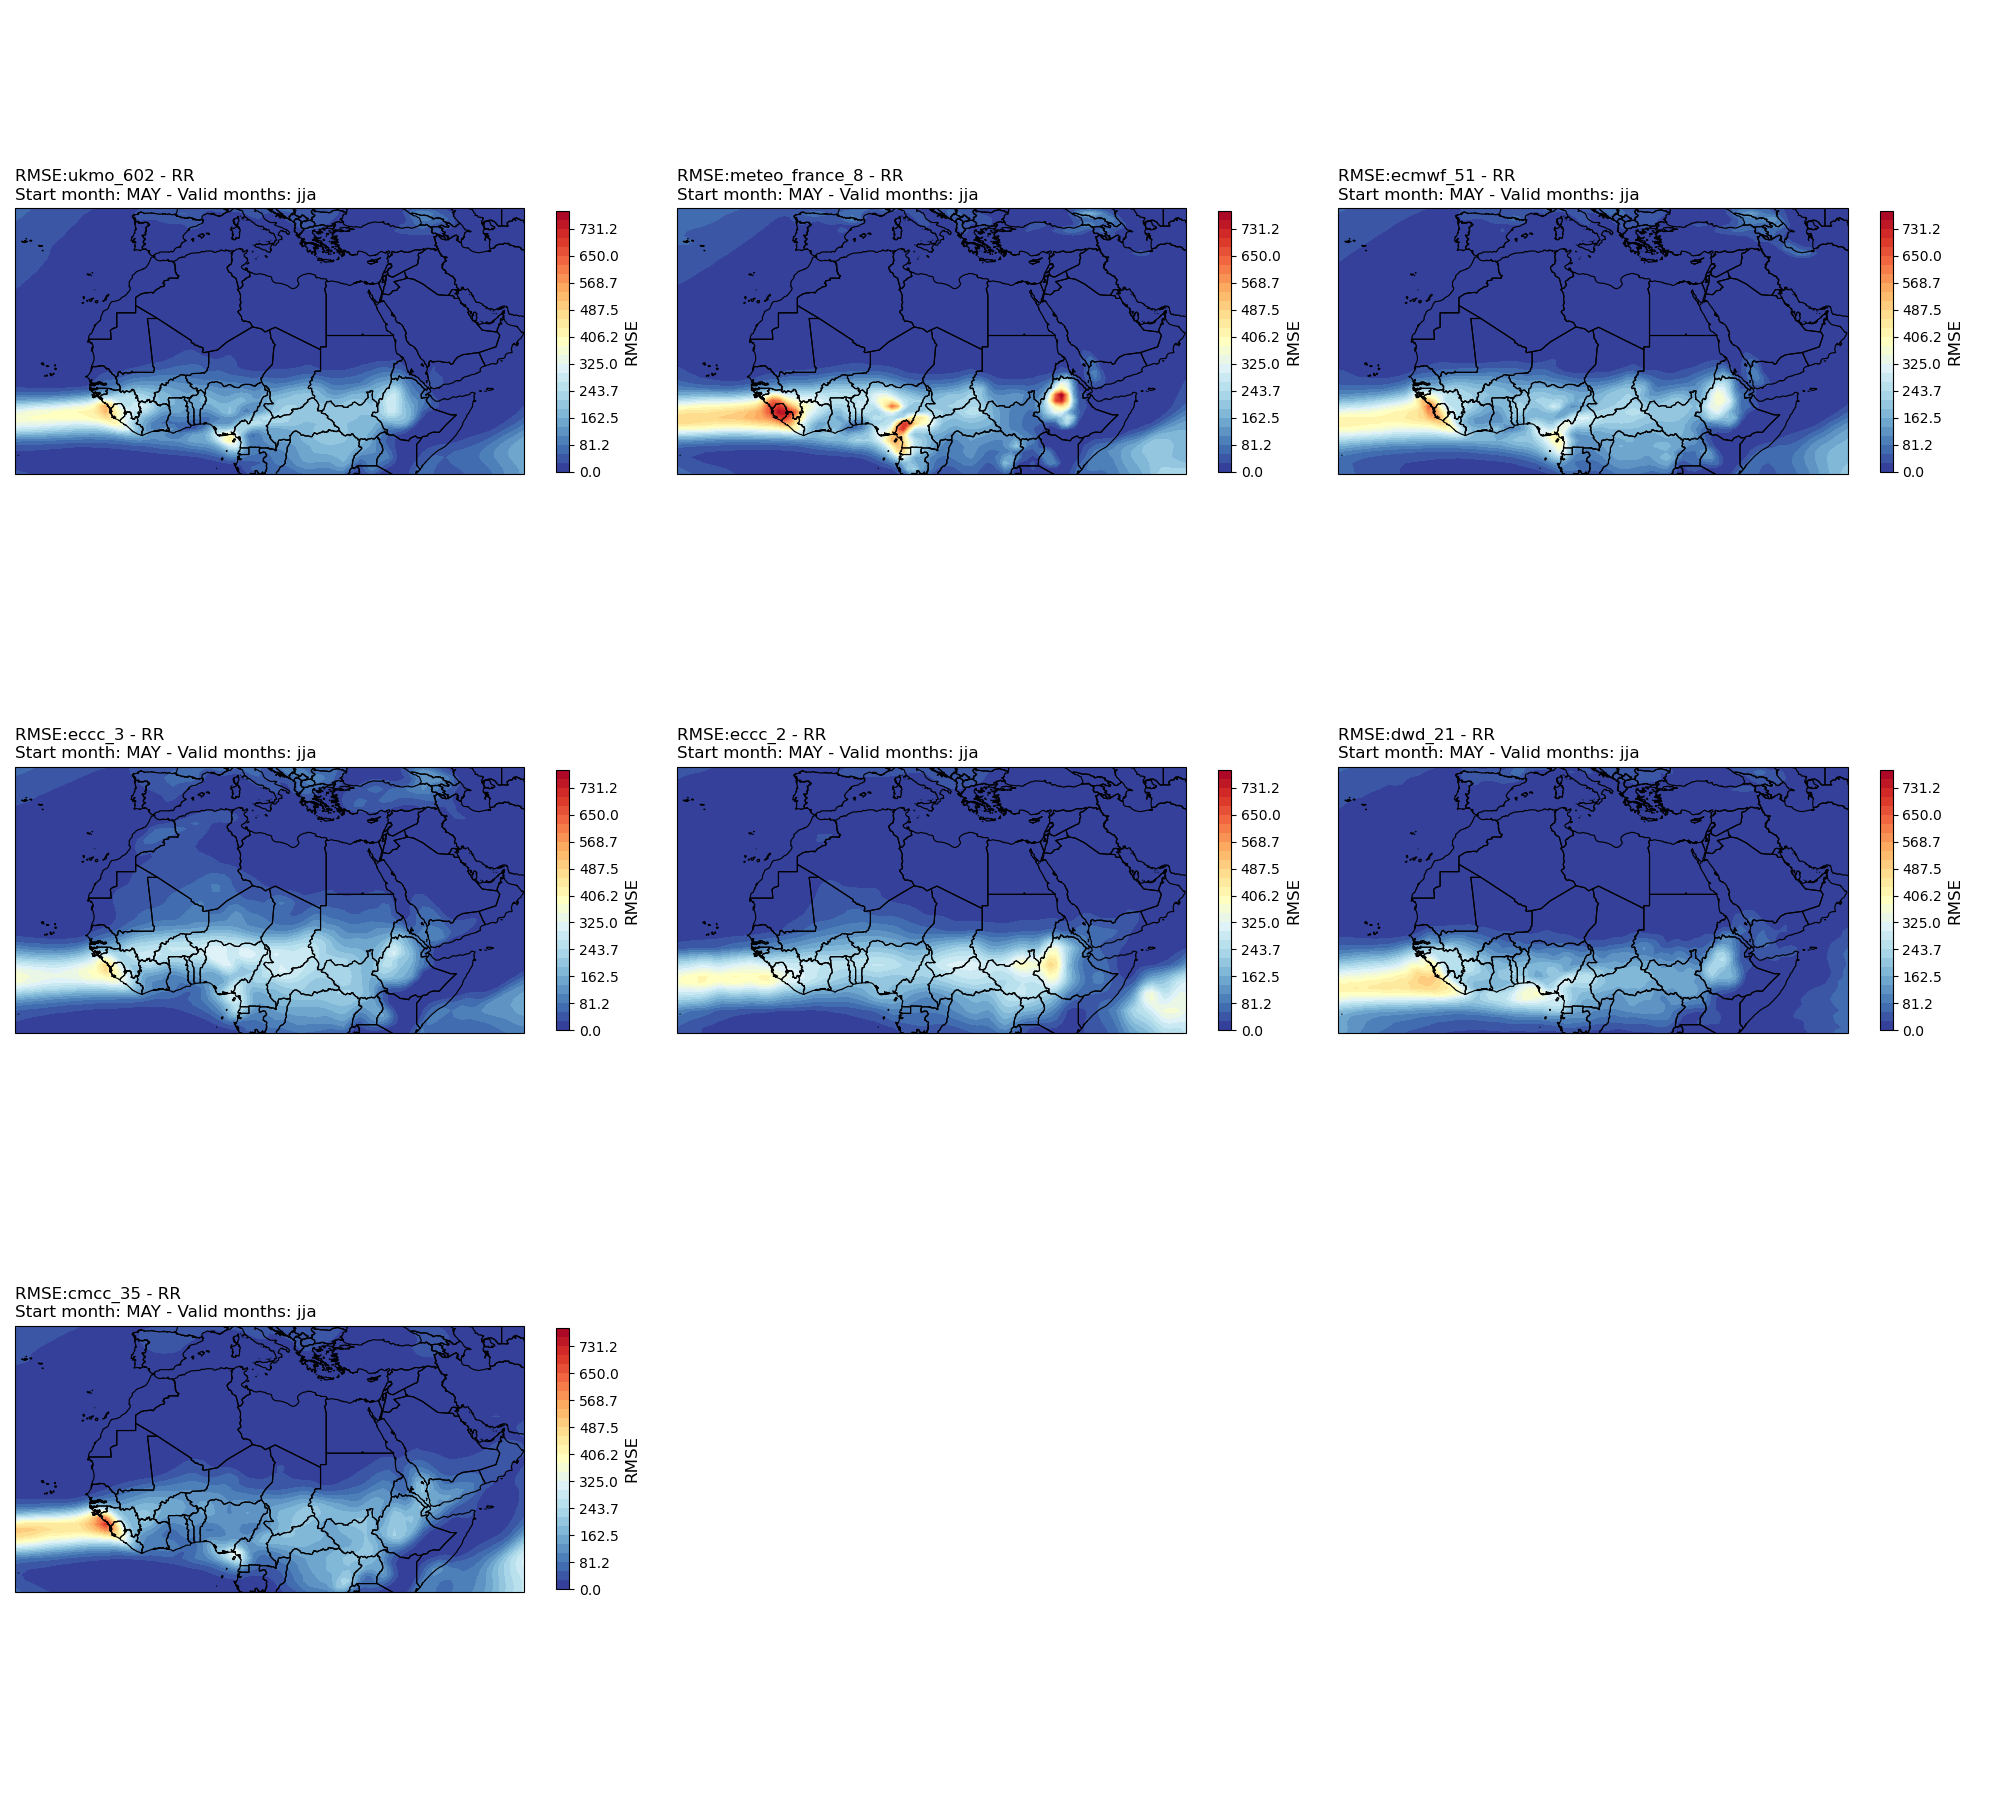
\includegraphics[scale=0.3]{plots/det/rmse/rmse_jja_RR.png}
\caption{3-months Rolling mean of RMSE in MENA Region for all centers JJA in mm}
\end{figure}

also for the spacial dimension, the RMSE stay stable and exhibit moderate performance for all centers. Thus, all models have almost the same skill and they are consistent with each other. We can see some isolated areas in the equator where the RMSE is very high reaching 731 mm for all centers especially \textbf{\textit{ECMWF and METEO-FRANCE}} for both DJF and JJA especially in JJA.

\begin{figure}[H]
\centering
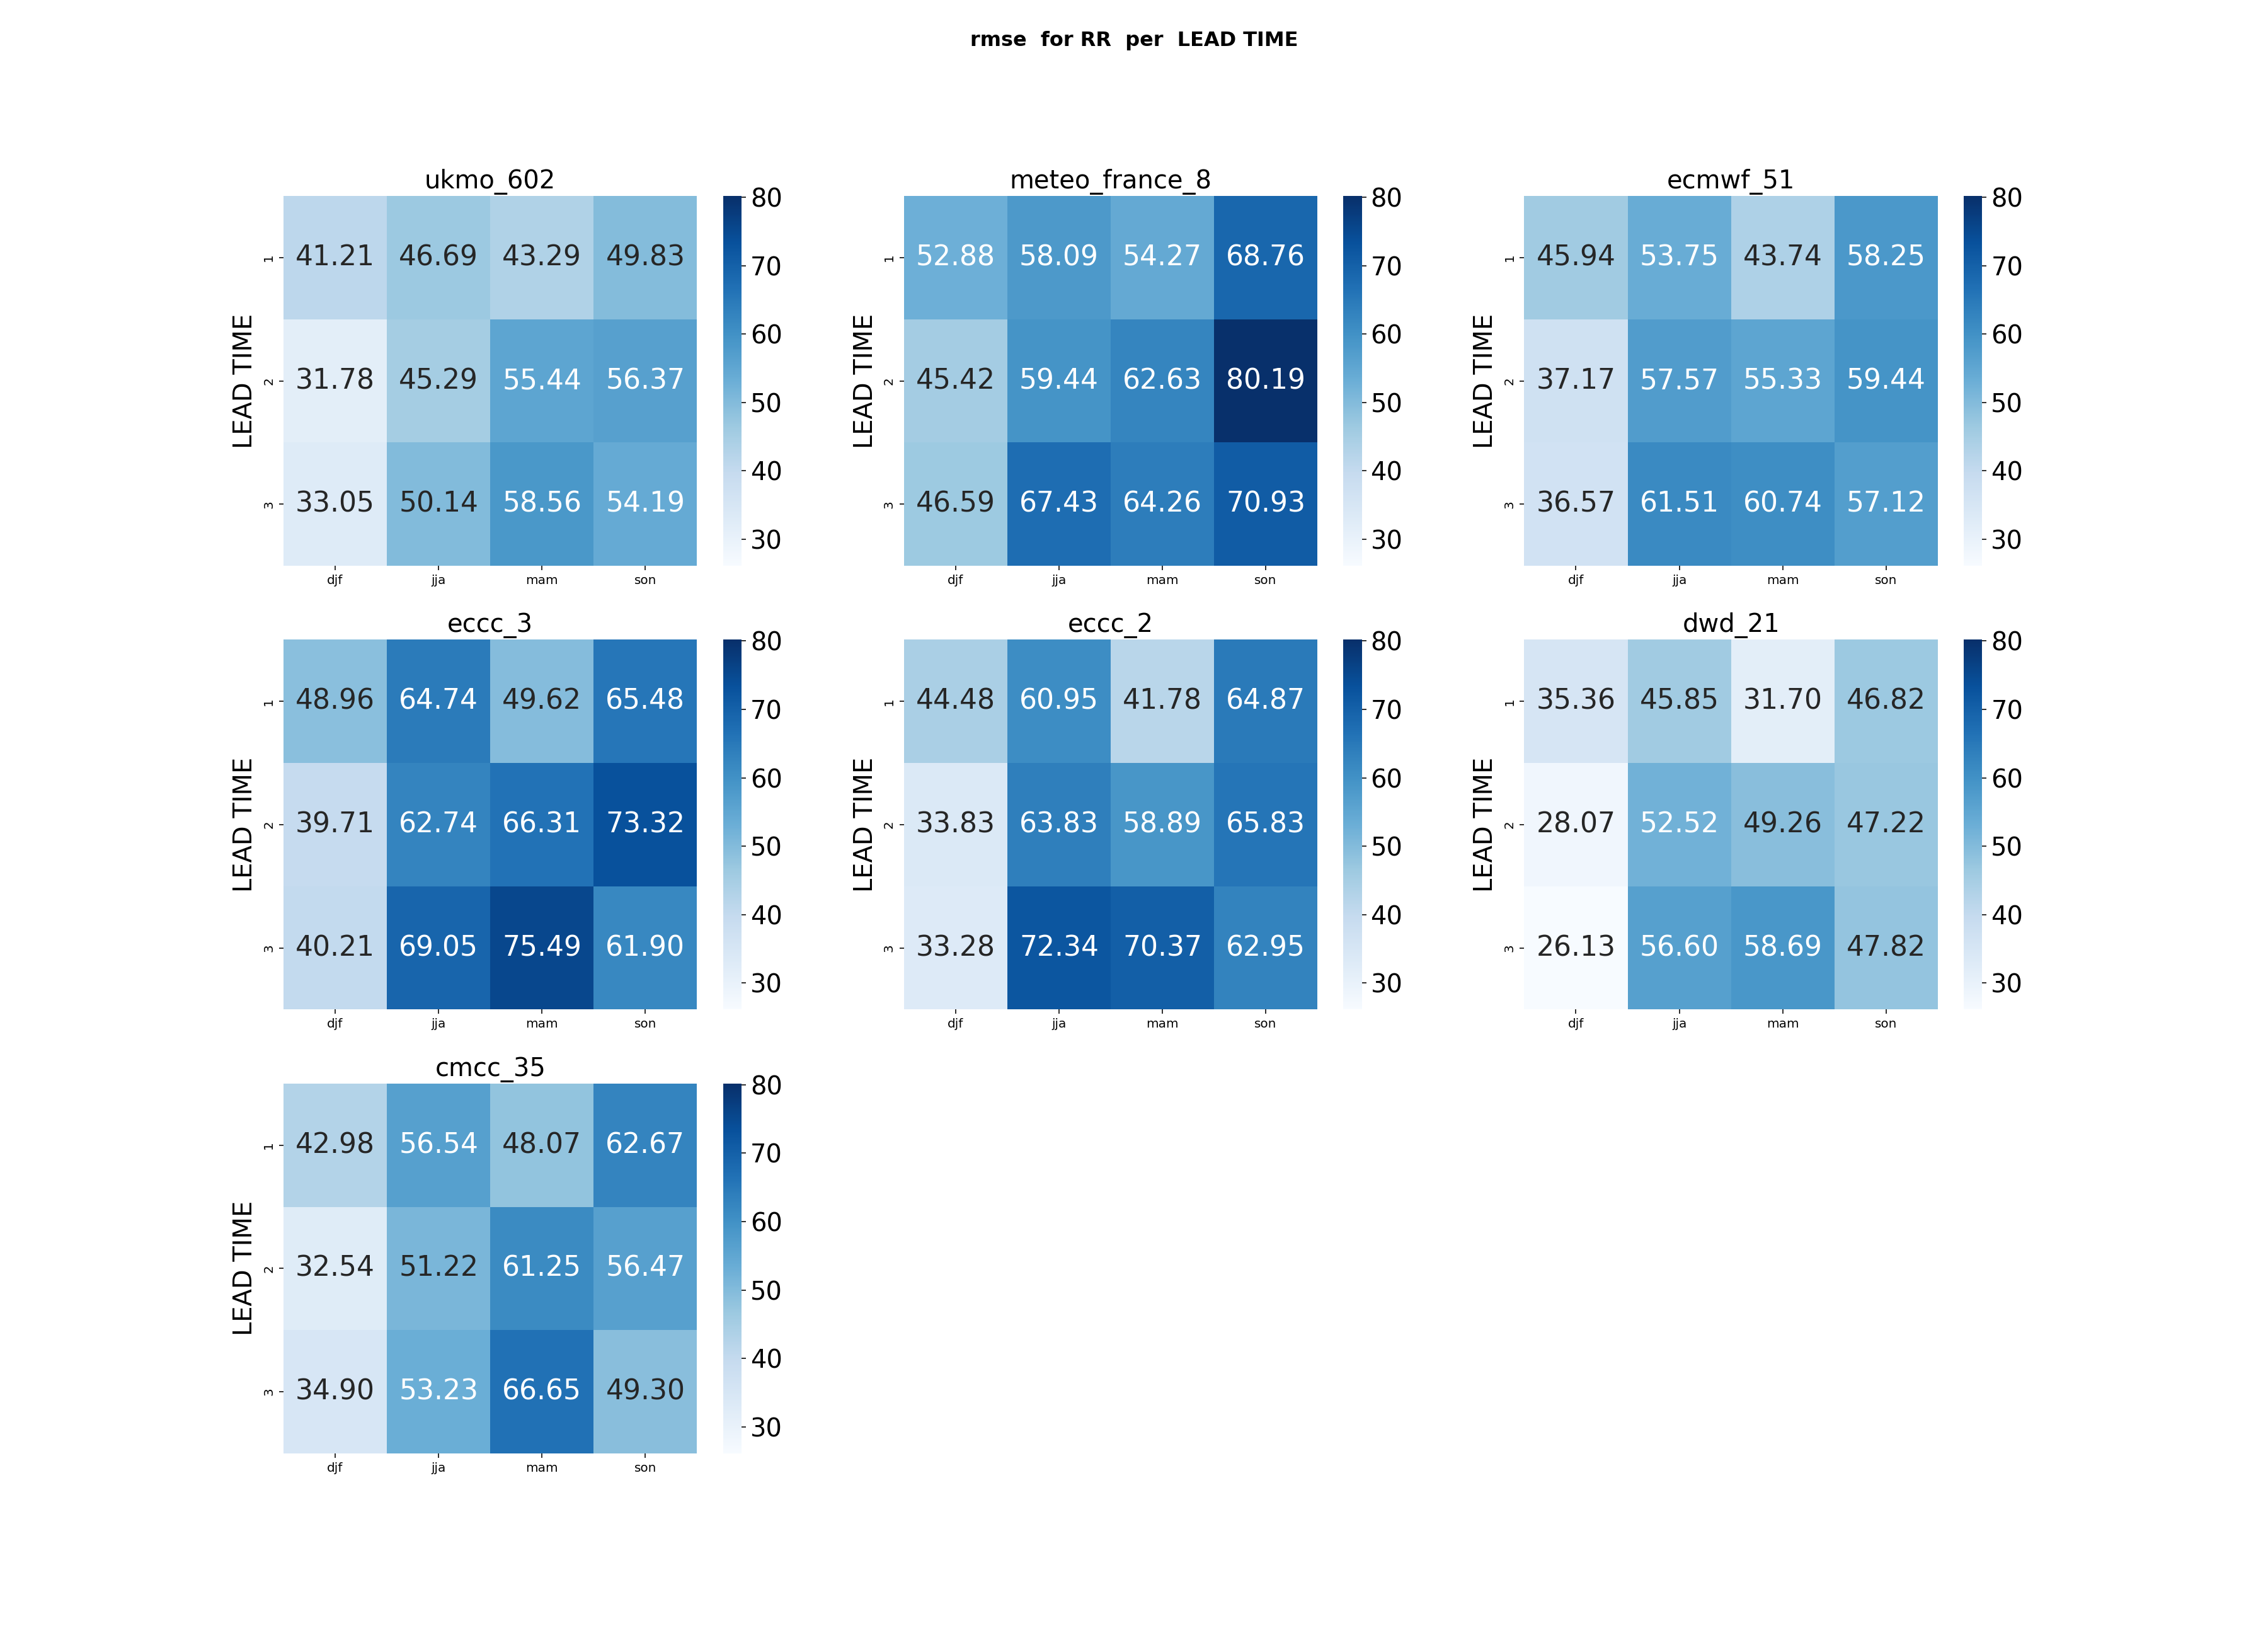
\includegraphics[scale=0.3]{plots/det/rmse/rmse_RR_mena.png}
\caption{heatmap of RMSE For RR in mm}
\end{figure}

for the Root Mean Squared Error, the best models shown in the heatmap above are \textbf{\textit{DWD, ECMWF and UKMO}} .The RMSE score demonstrate a moderate performance for all models especially \textbf{\textit{DWD, ECMWF and UKMO}}. The performance is stable over lead-times and it is much better for djf in all centers with values between 26 and 35 for \textbf{\textit{DWD}} . The SON exhibit the biggest RMSE for all centers, with values around 70 in \textbf{\textit{METEO-FRANCE}}.

\paragraph{focus on North Africa} : 
\begin{figure}[H]
\centering
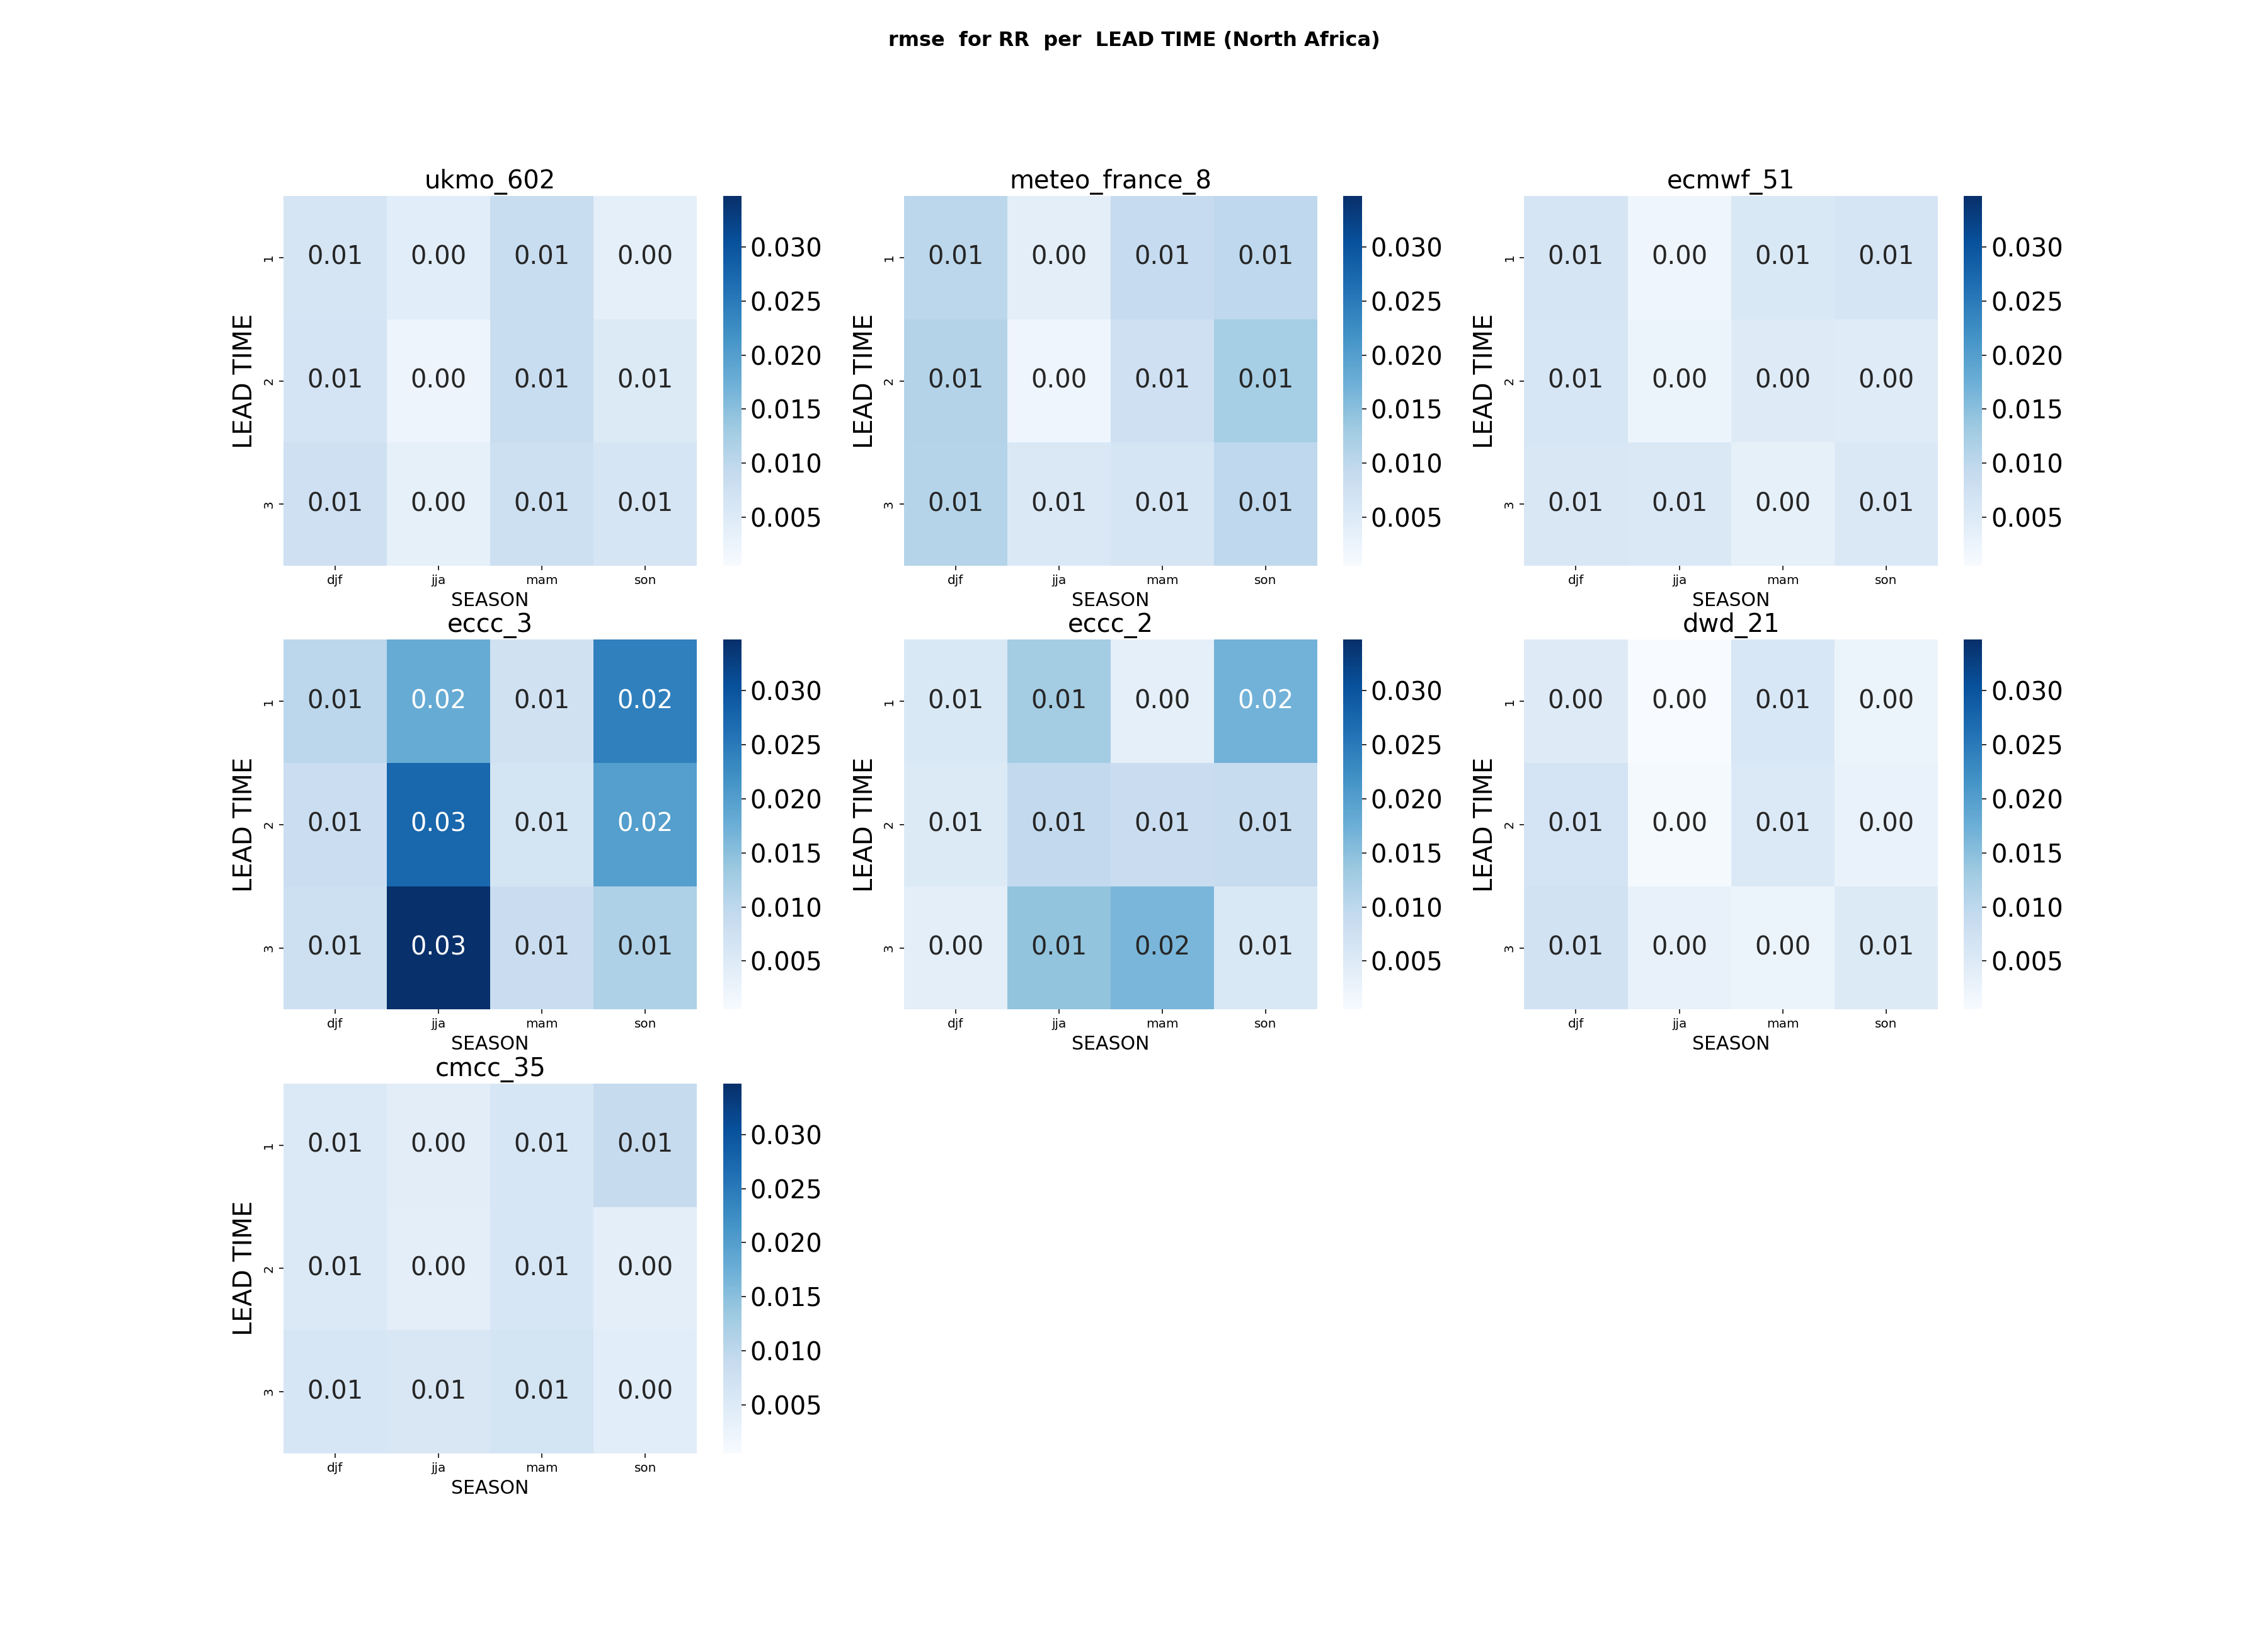
\includegraphics[scale=0.3]{plots/det/rmse/rmse_RR_NorthAfrica.png}
\caption{heatmap of RMSE For RR in mm (North Africa)}
\end{figure}

the RMSE is much better for North africa, the score is good over all lead-times and seasons. The centers, \textbf{\textit{ecmwf, ukmo and dwd}} show very good performance.

\vspace{1.5cm}
\paragraph{focus on Arabian Peninsula}:

\begin{figure}[H]
\centering
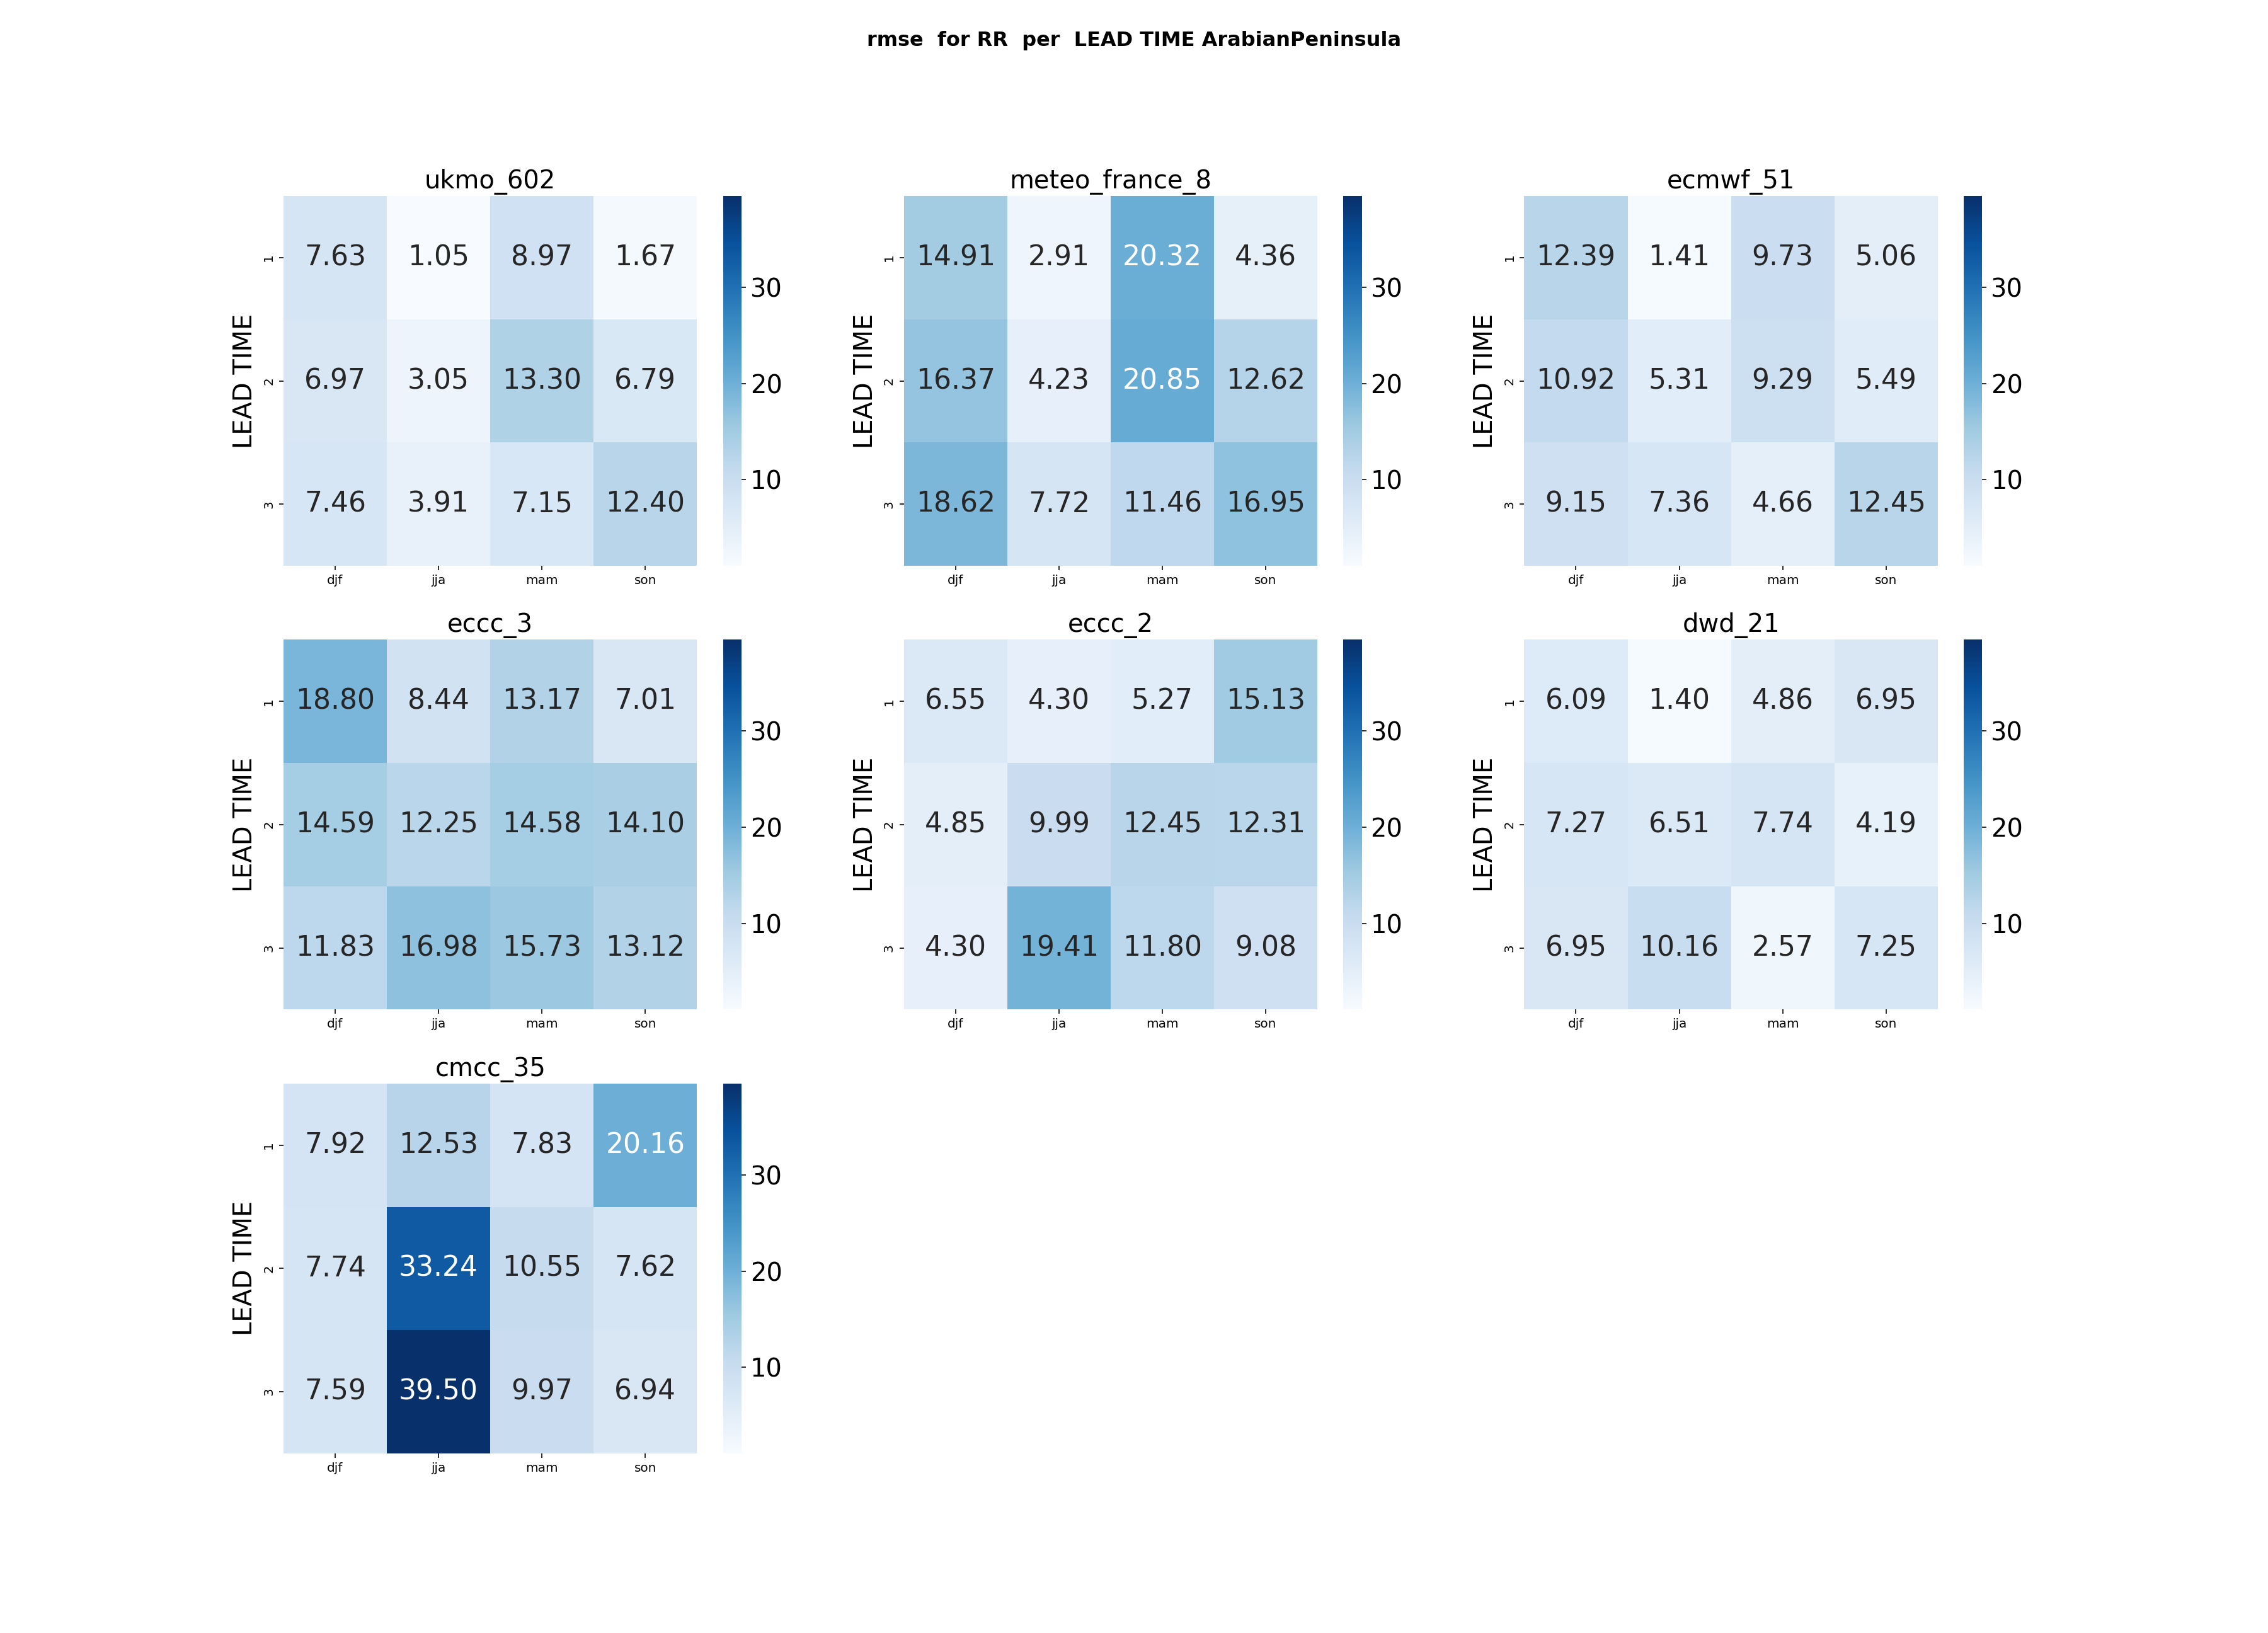
\includegraphics[scale=0.3]{plots/det/rmse/rmse_RR_ArabianPeninsula.png}
\caption{heatmap of RMSE For RR in mm (Arabian Peninsula)}
\end{figure}

In the same way as North Africa, the RMSE for the Arabian Peninsula is much better than mena. The centers, \textbf{\textit{ecmwf, ukmo and dwd}} show very good performance.

\subsubsection{Coefficient of Determination (\( R^2 \))}
for precipitation, the R-SQUARED is very low, the maximum value is less than 0.1. However, the ecmwf is the best in term of R-SQUARED. for DJF,JJA and MAM the highest performance is in the first Lead-time, and it decrease along time, But for SON the best score is in the second Lead-time for all centers.
\begin{figure}[H]
	\centering
	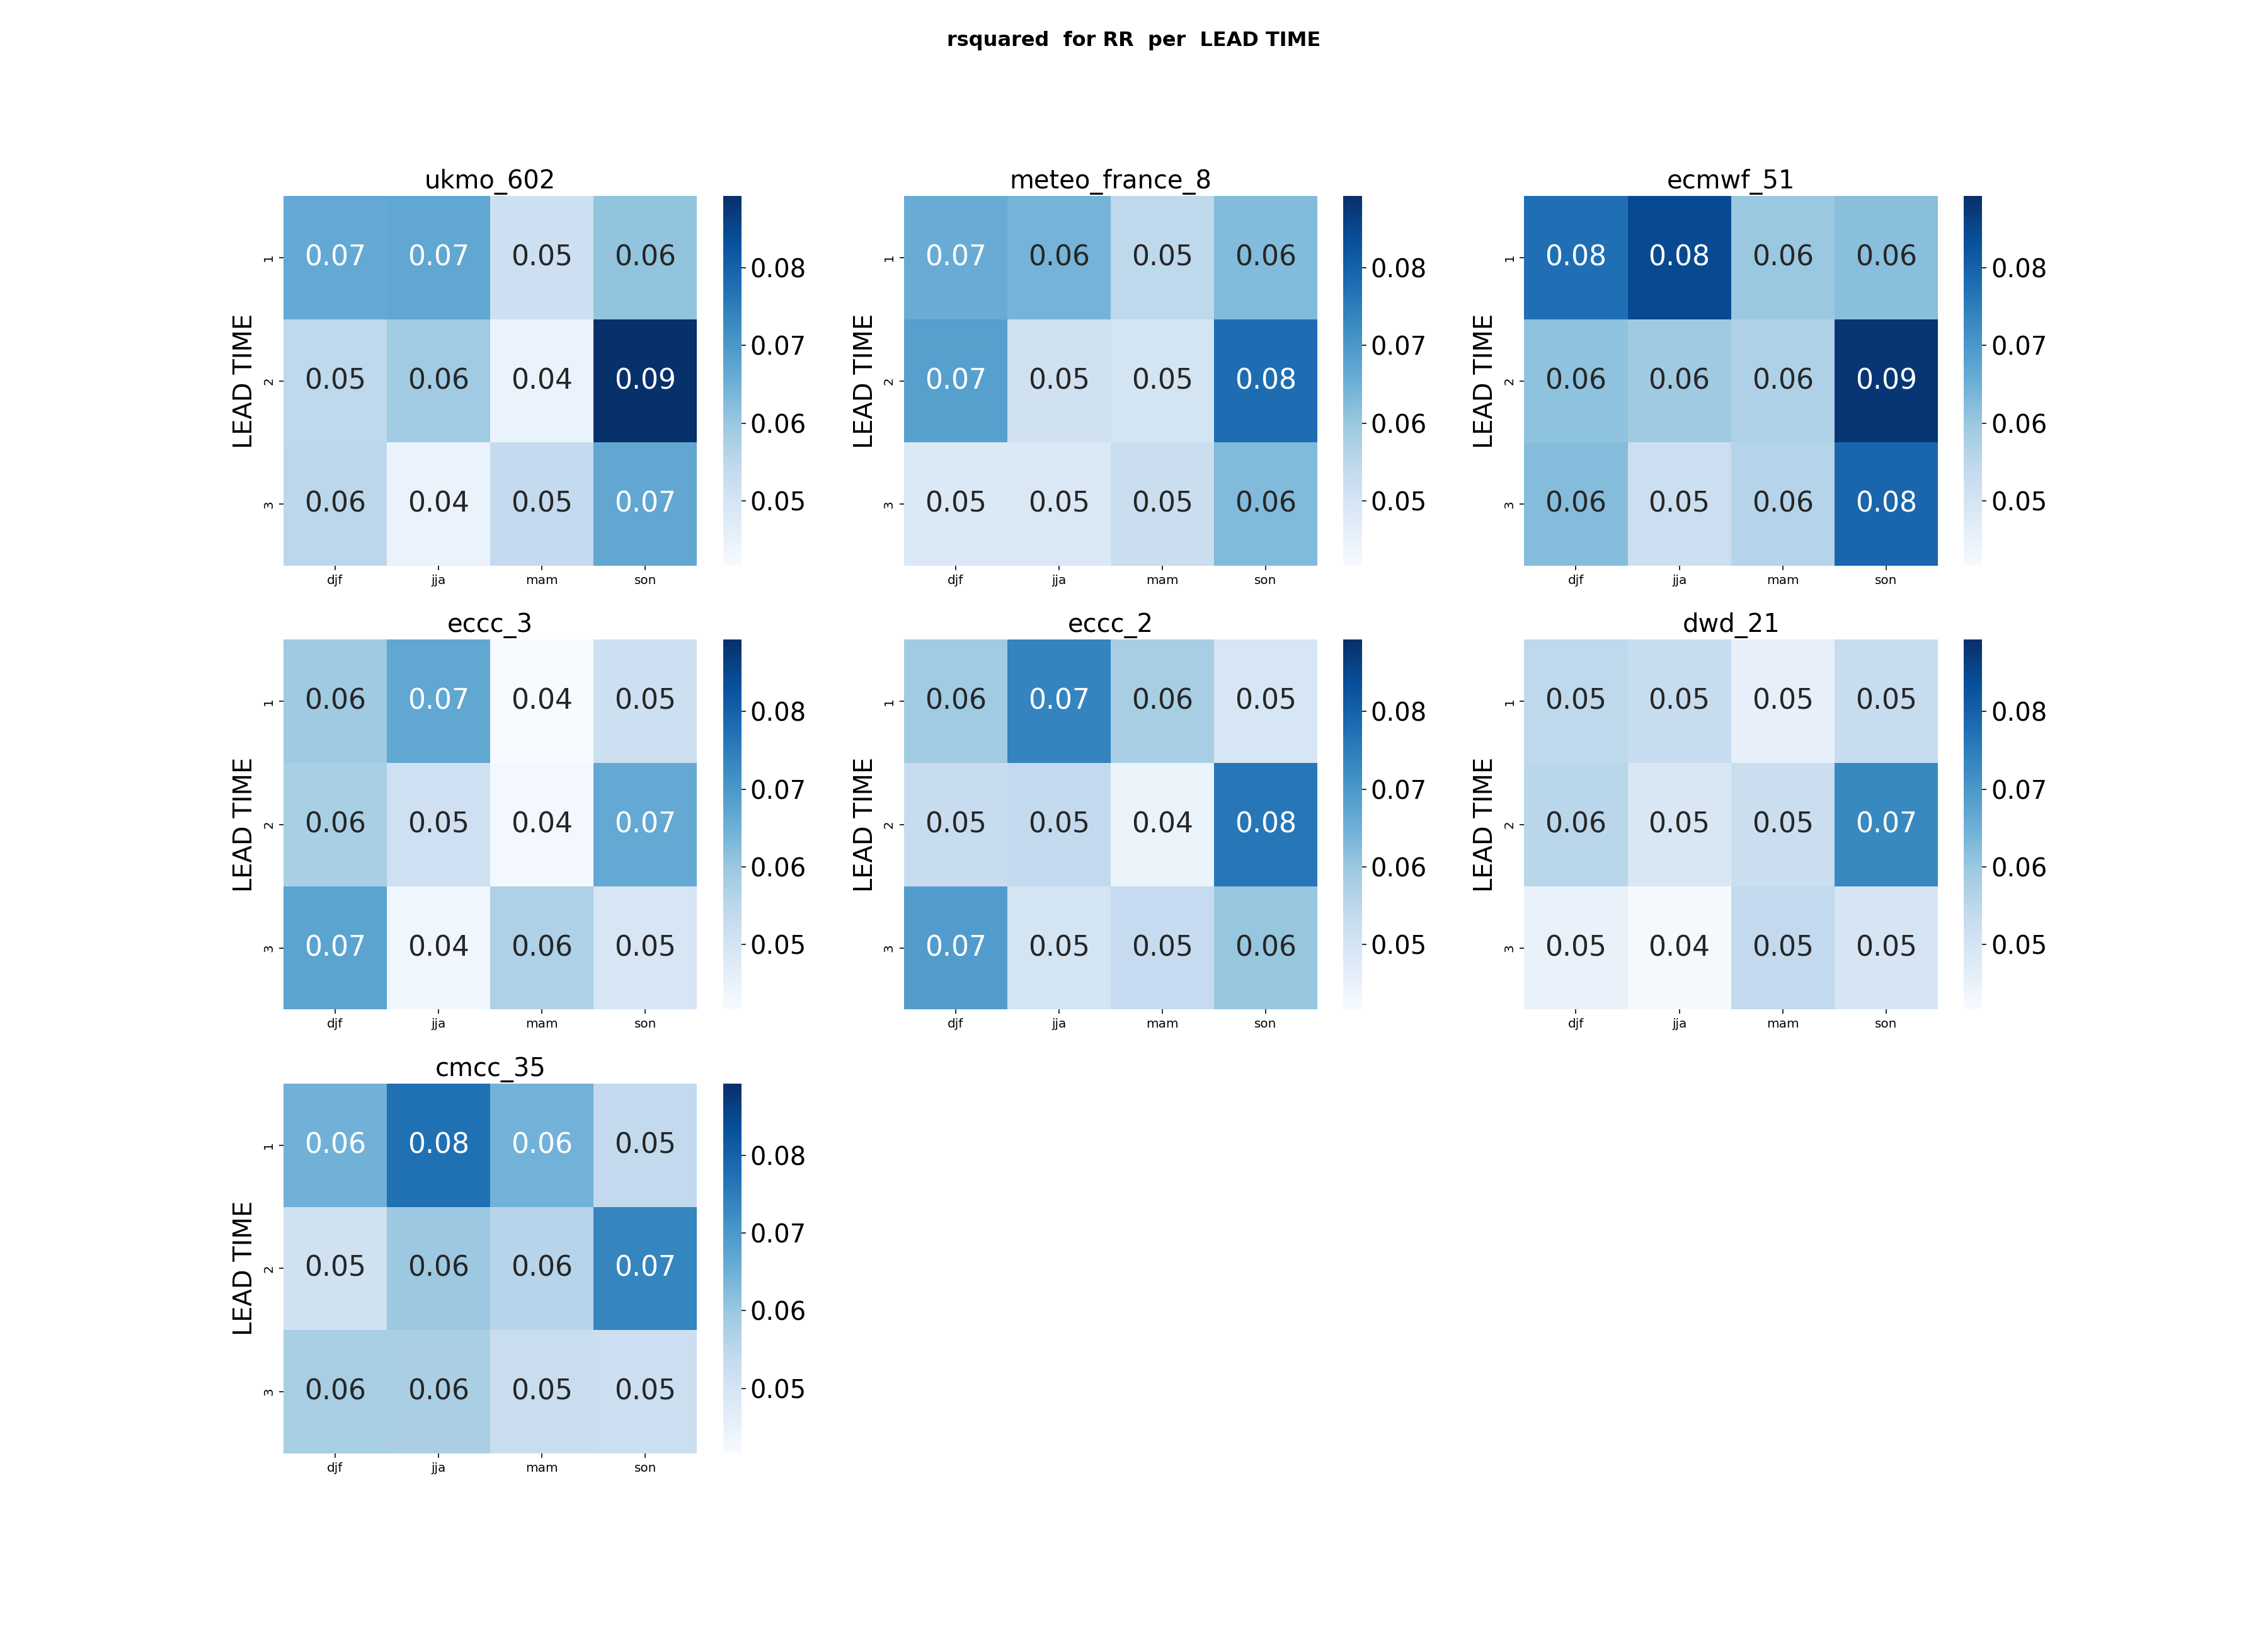
\includegraphics[scale=0.25]{plots/det/rsquared/rsquared_RR_mena.png}
	\caption{The Heatmap of rsquared for Precipitations in the mena region for every period \textbf{\textit{(1 for perfect RSQUARED)} }}
\end{figure}


\begin{figure}[H]
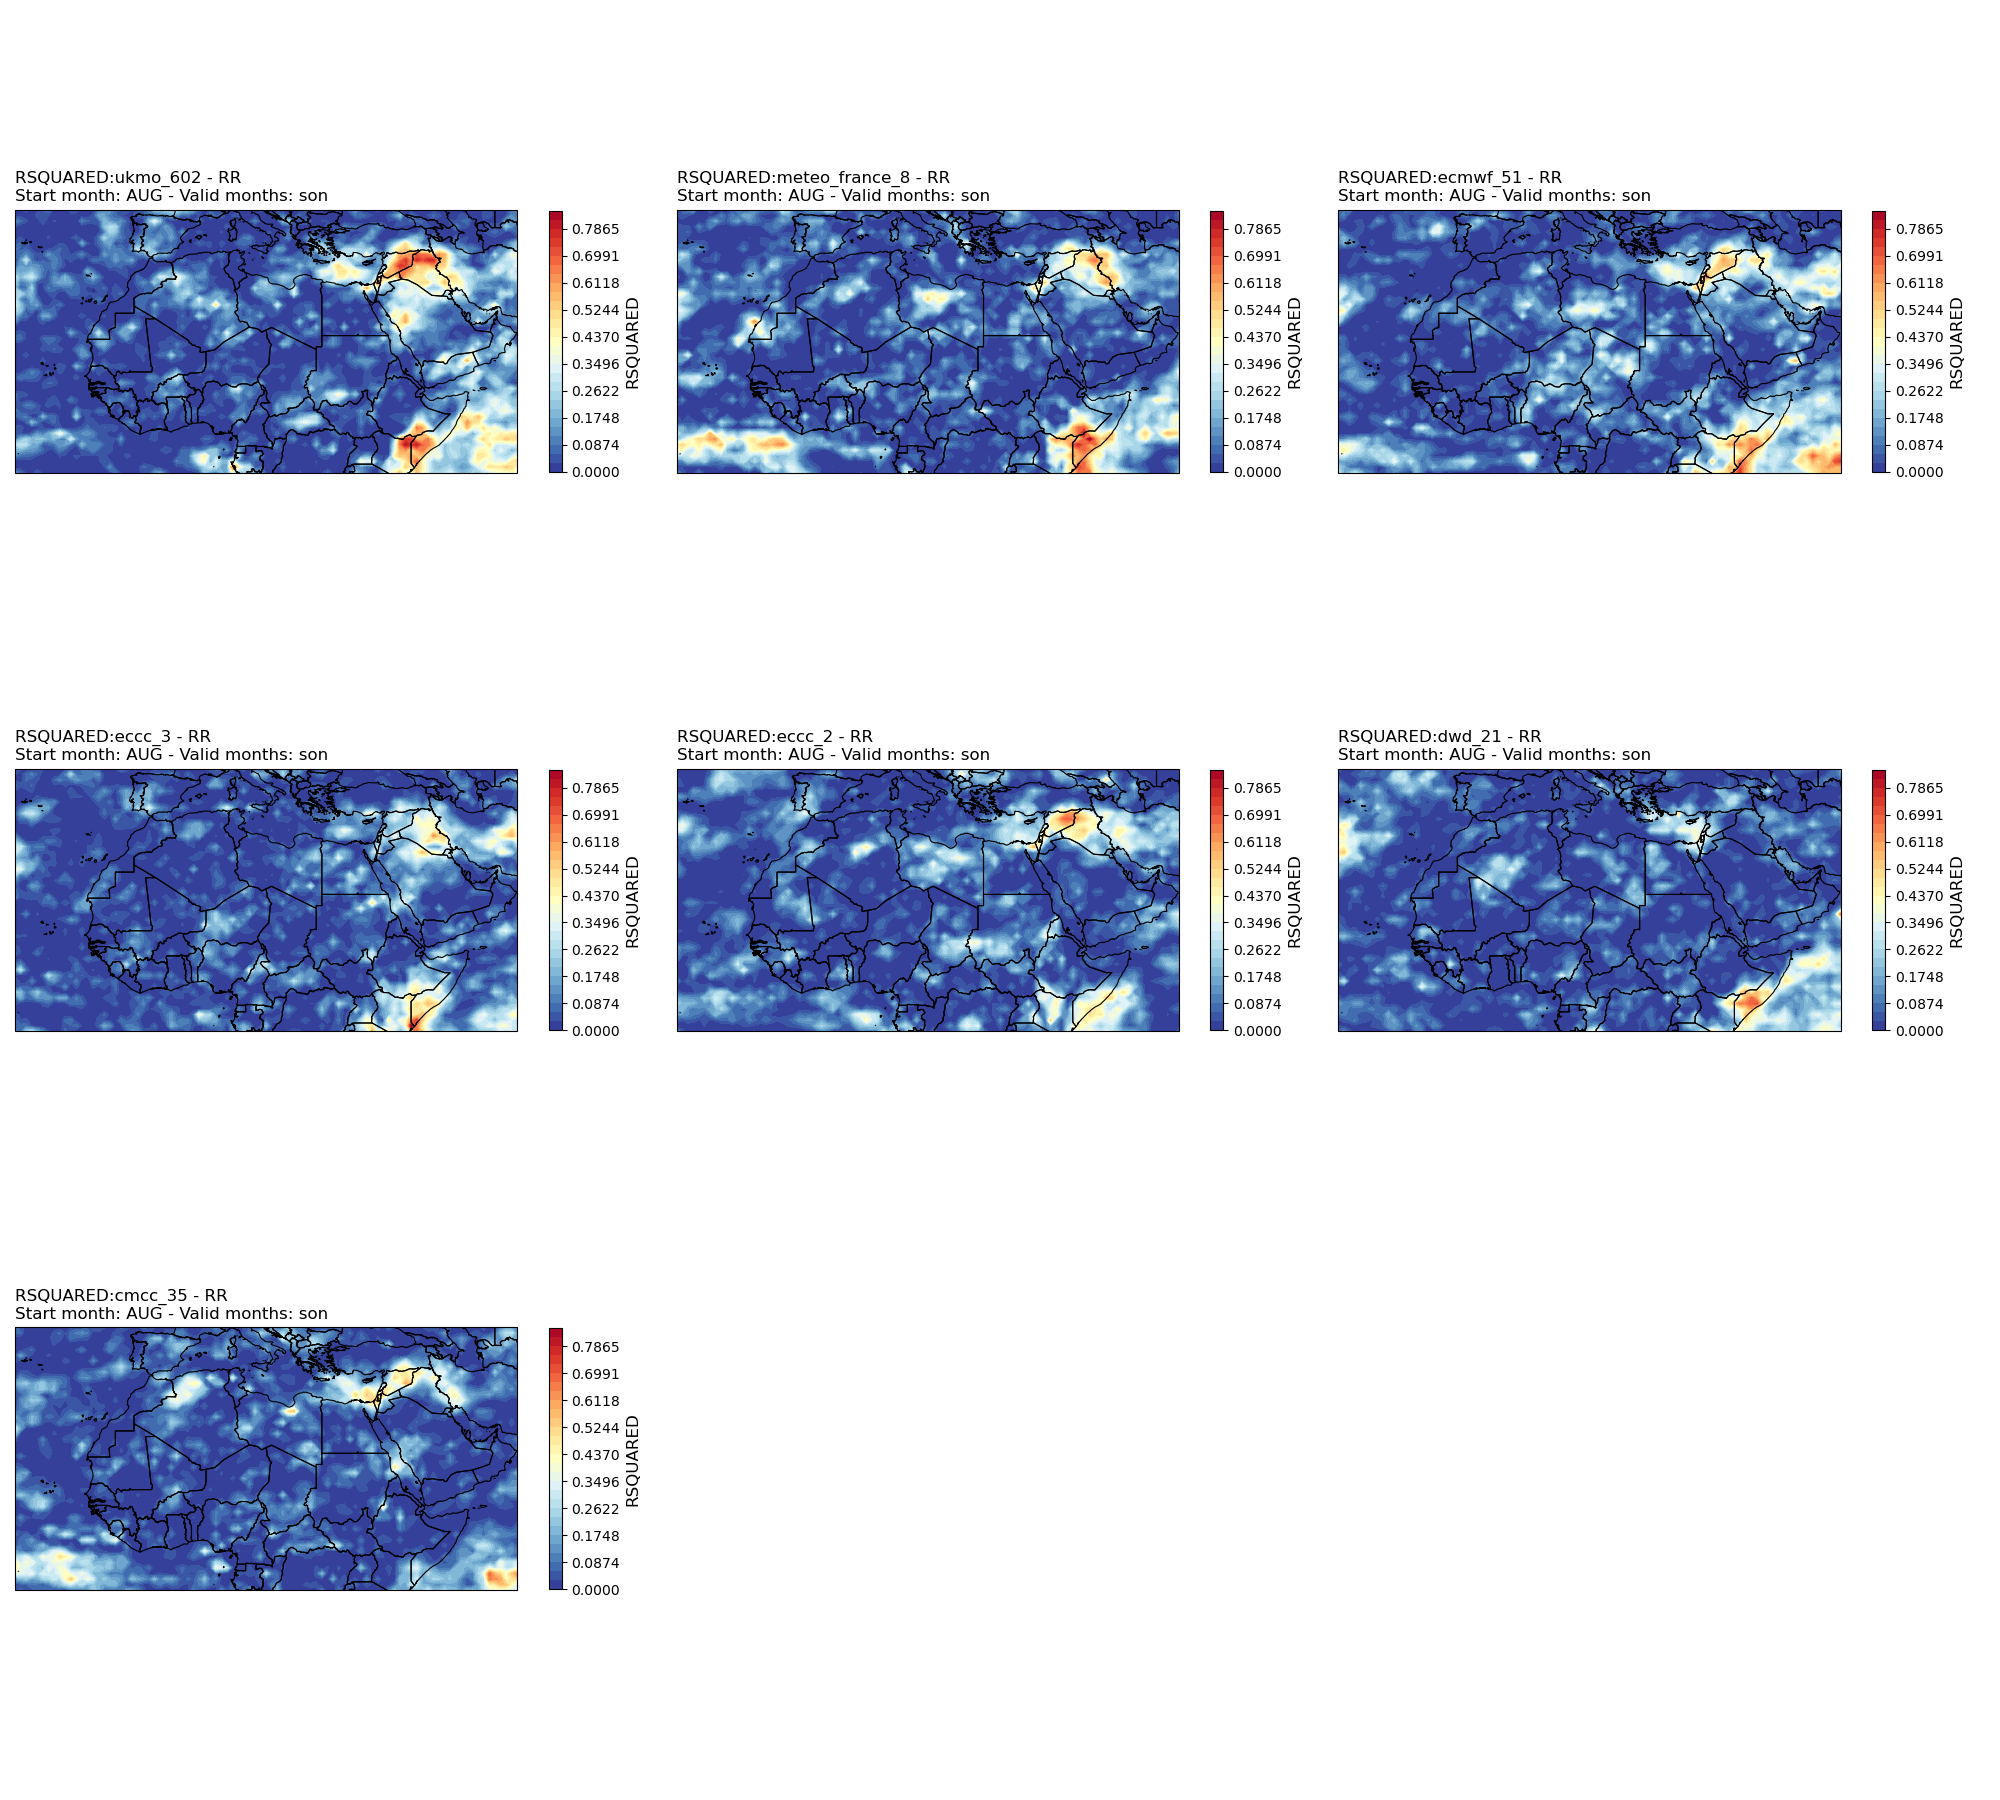
\includegraphics[scale=0.3]{plots/det/rsquared/rsquared_son_RR.png}
\caption{3-months Rolling mean of RSQUARED in MENA Region for all centers SON}
\end{figure}

there is some isolated zones where the r-squared is good especially in Syria, Irak, Jordan ,Palestine  and East Africa, this high performance is observed in all centers. For the rest of the MENA region the performance is very bad with score near to 0. Hence, there is no constant pattern for the R-SQUARED, the spacial variation is very high for all centers.

\paragraph{focus on North Africa}

there is no big difference in North Africa.


\vspace{1.5cm}
\paragraph{focus on Arabian Peninsula}:


\begin{figure}[H]
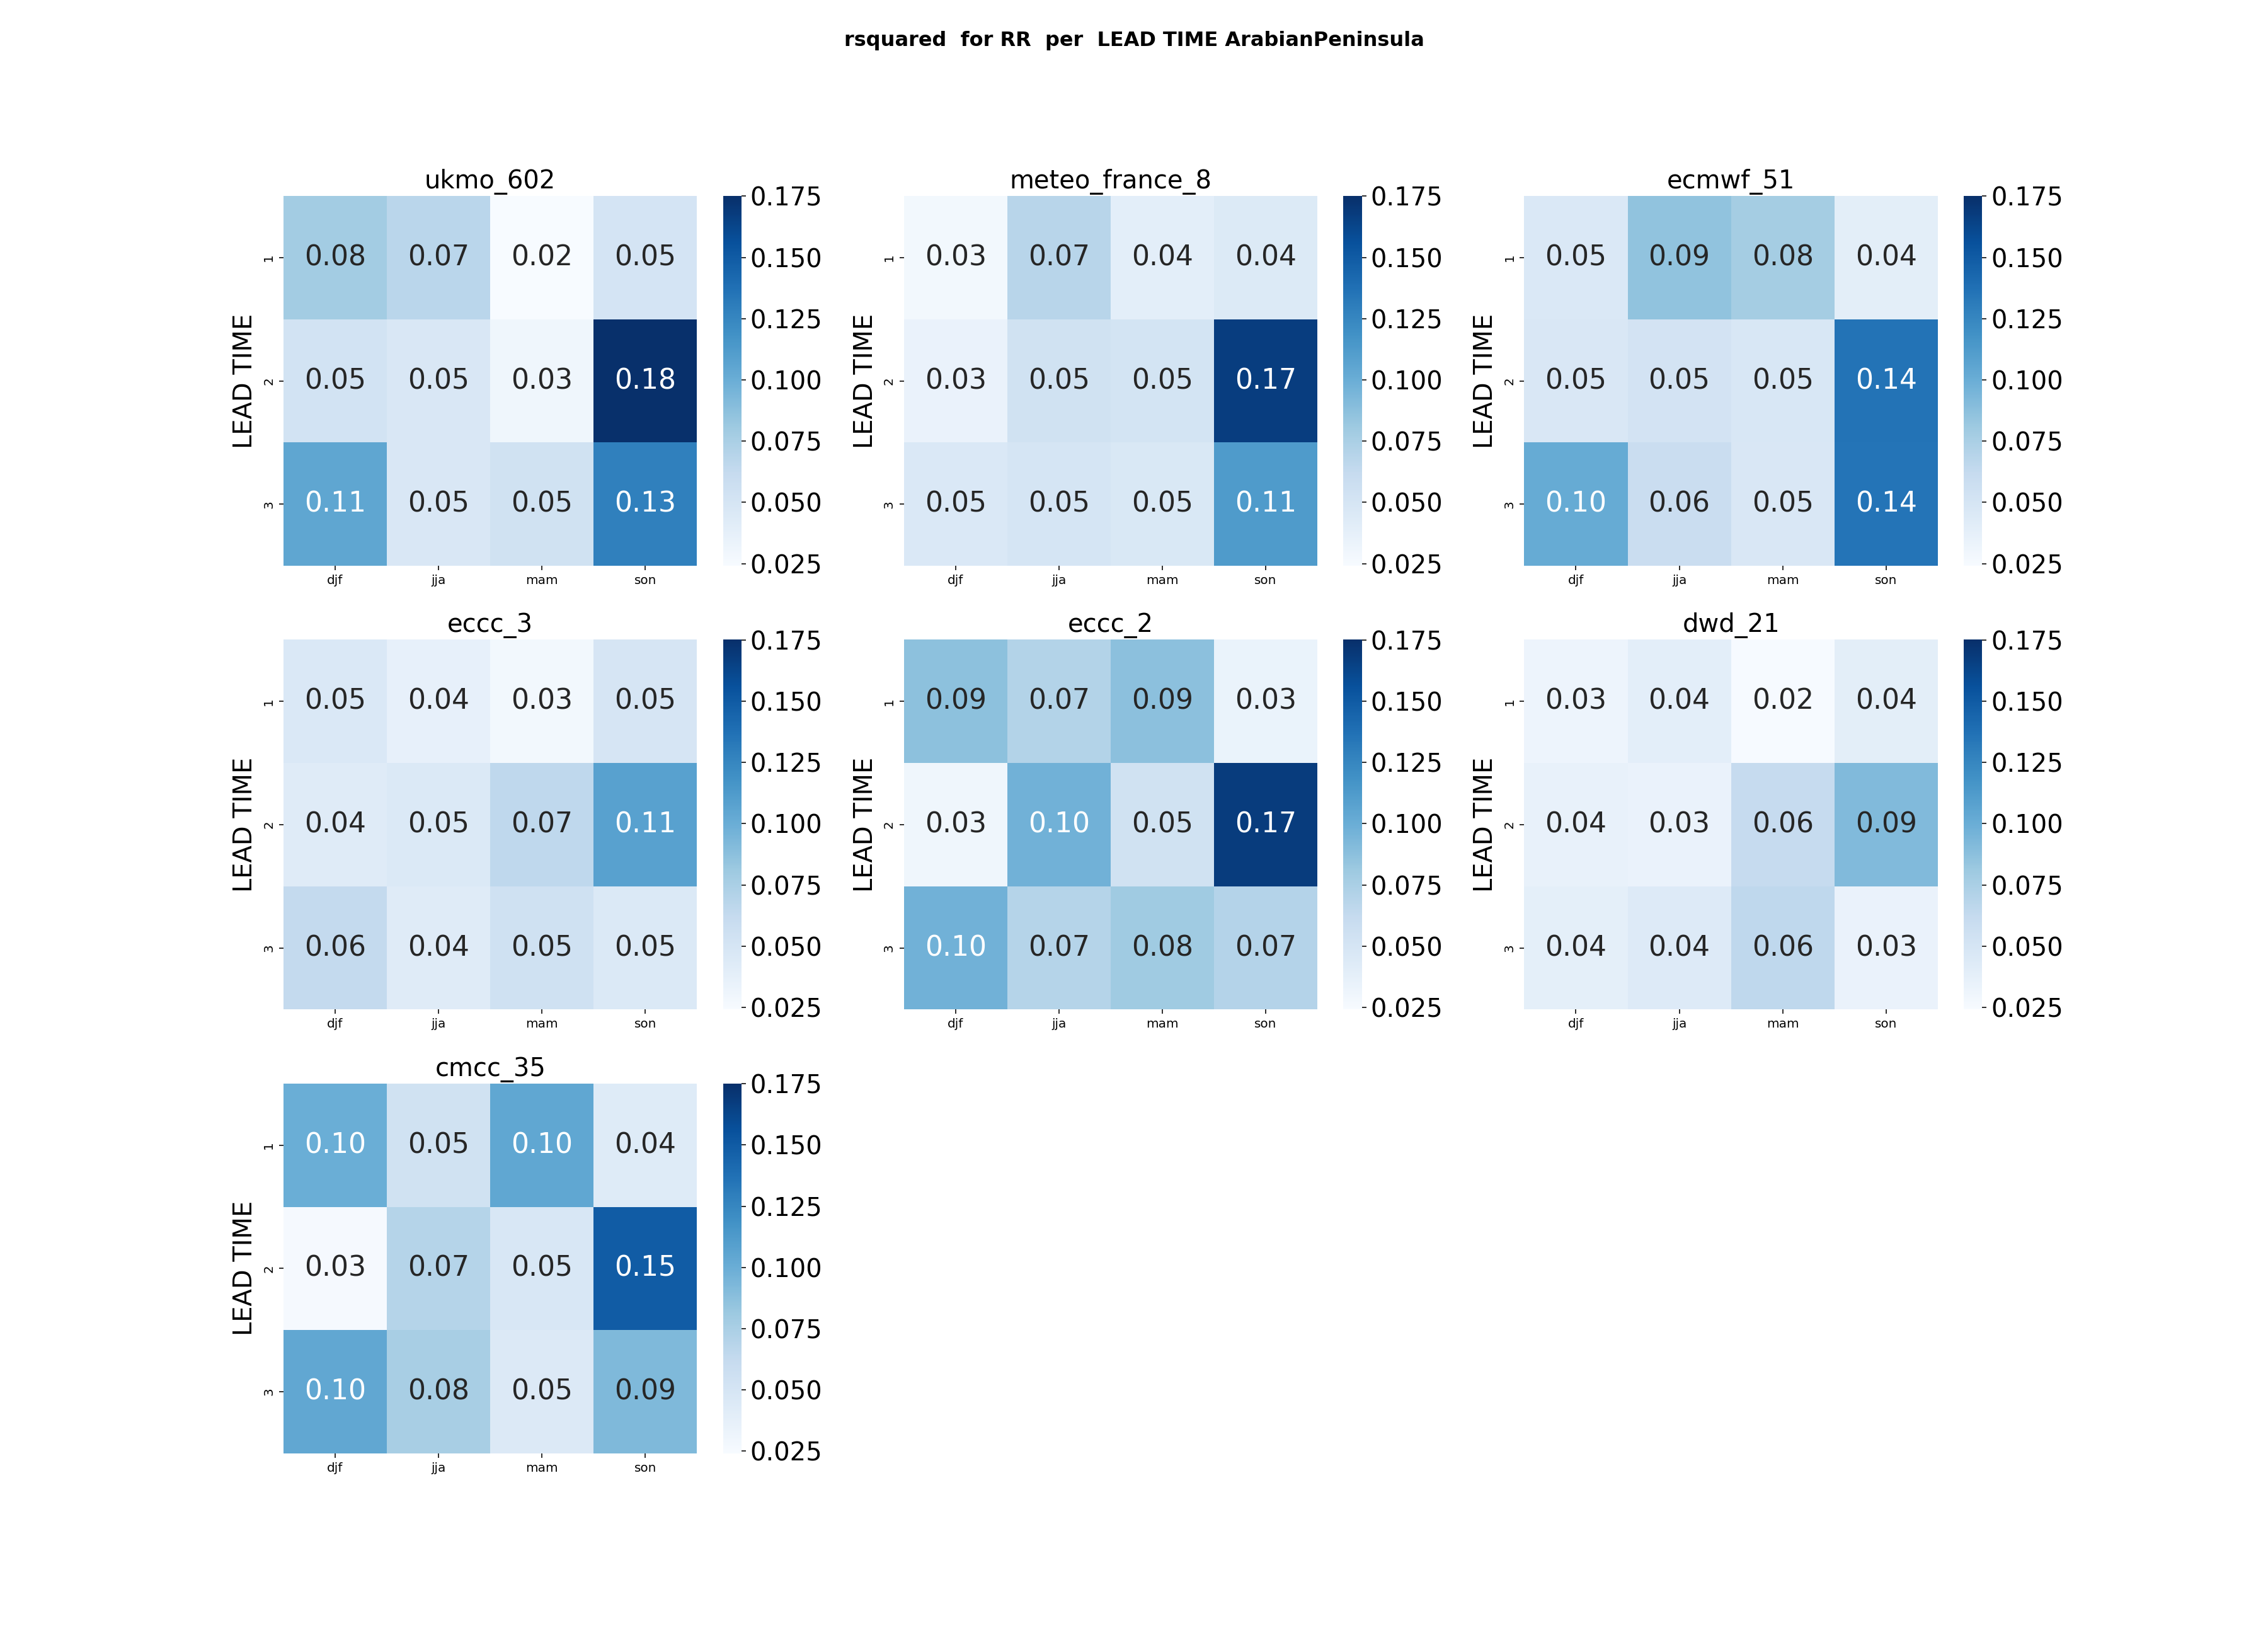
\includegraphics[scale=0.3]{plots/det/rsquared/rsquared_RR_ArabianPeninsula.png}
\caption{Heatmap of RR  RSQUARED in MENA Region for all centers Arabian Peninsula}
\end{figure}

the R-SQUARED for the Arabian Peninsula shows a little improvement.
\subsection{Probabilistic Evaluation Metrics}

\subsubsection{The Brier Score (BS)}

\begin{figure}[H]
    \centering
    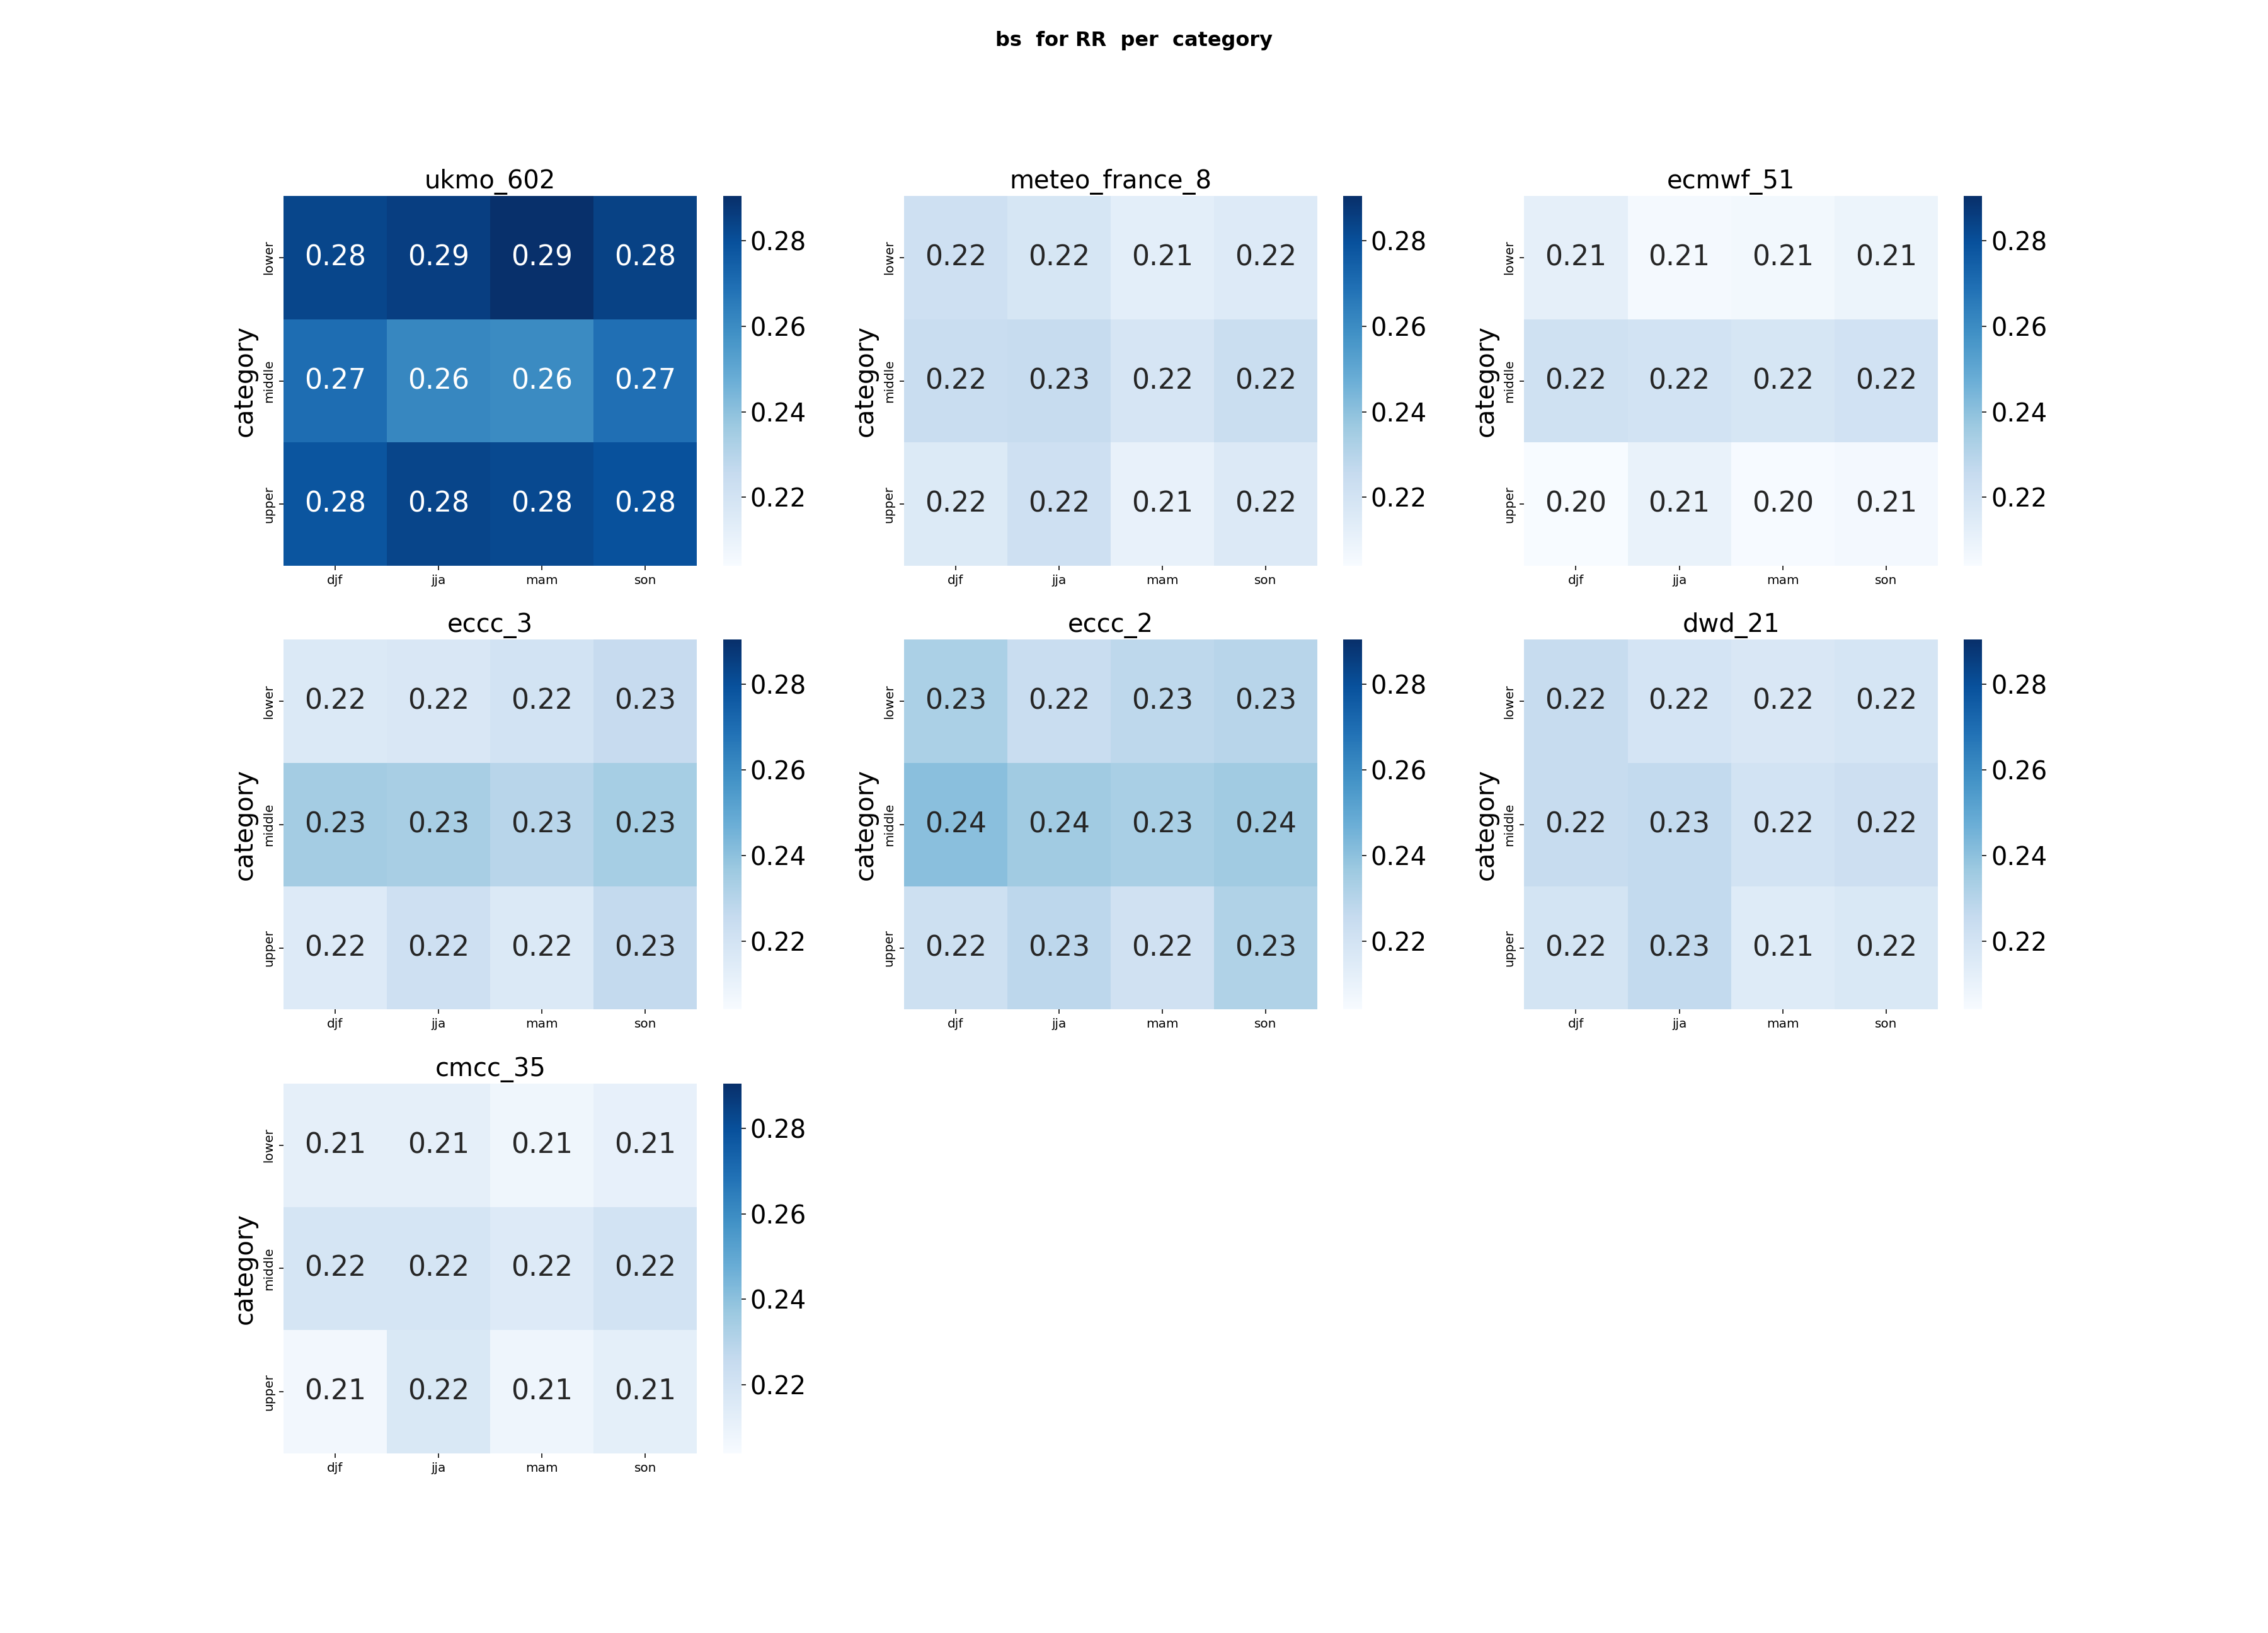
\includegraphics[scale=0.25]{plots/prob/bs/bs_RR_category.png}
    \caption{The Heatmap of Brier Score for each category  . \textbf{\textit{(0 represents perfect BS)}}}
\end{figure}

for the analysis per category, we can see in the figure above that all centers exhibit good performance in term of Brier Score. Overall, the middle tercile shows lower performance (higher Brier Score) for all centers. 
the figure below shows the analysis per lead-time. the same result is found, but the \textbf{\textit{ECMWF,METEO-FRANCE and CMCC-35}} are the best models in Brier Score for lead-time analysis.The performance stay stable along time which is a reliable signal. Despite the UKMO have the lower performance, it stays close to the other centers, the difference isn't so wide. 
In general, the performance stays stable over category, lead-time and space.


\begin{figure}[H]
    \centering
    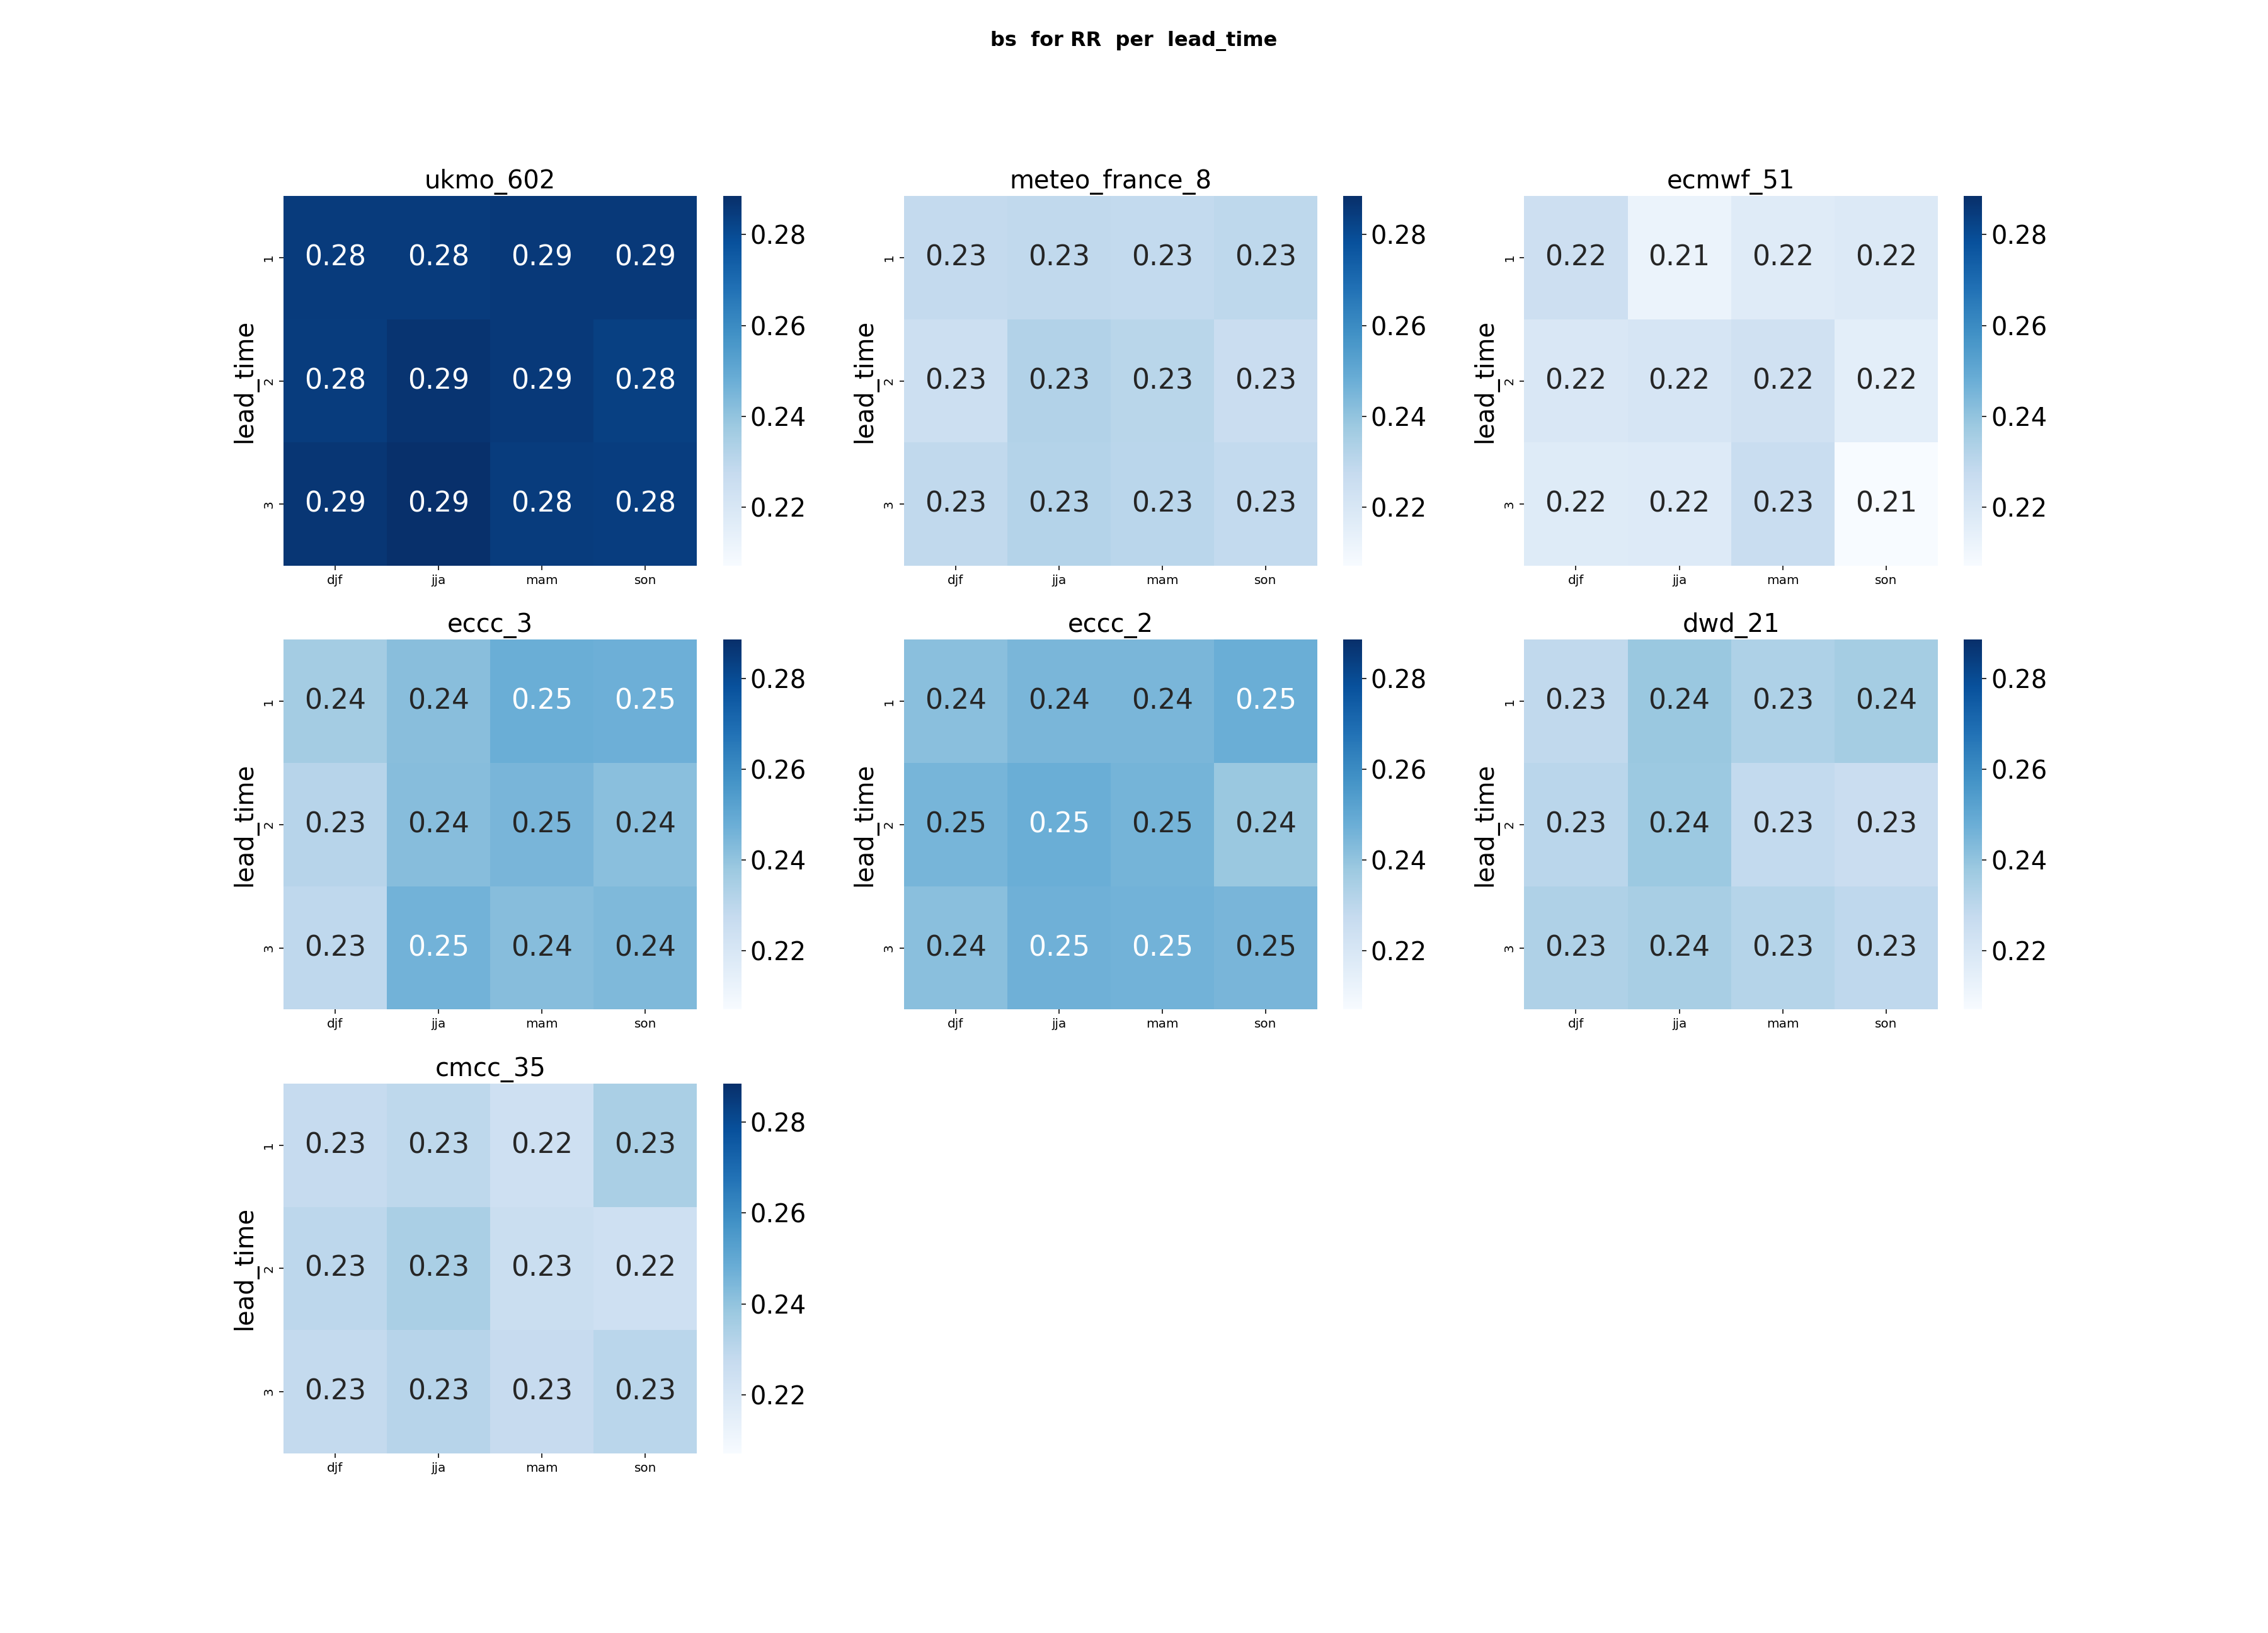
\includegraphics[scale=0.25]{plots/prob/bs/bs_RR_lead_time.png}
    \caption{The Heatmap of Brier Score for lead-time. \textbf{\textit{(0 represents perfect BS)}}}
\end{figure}


\begin{figure}[H]
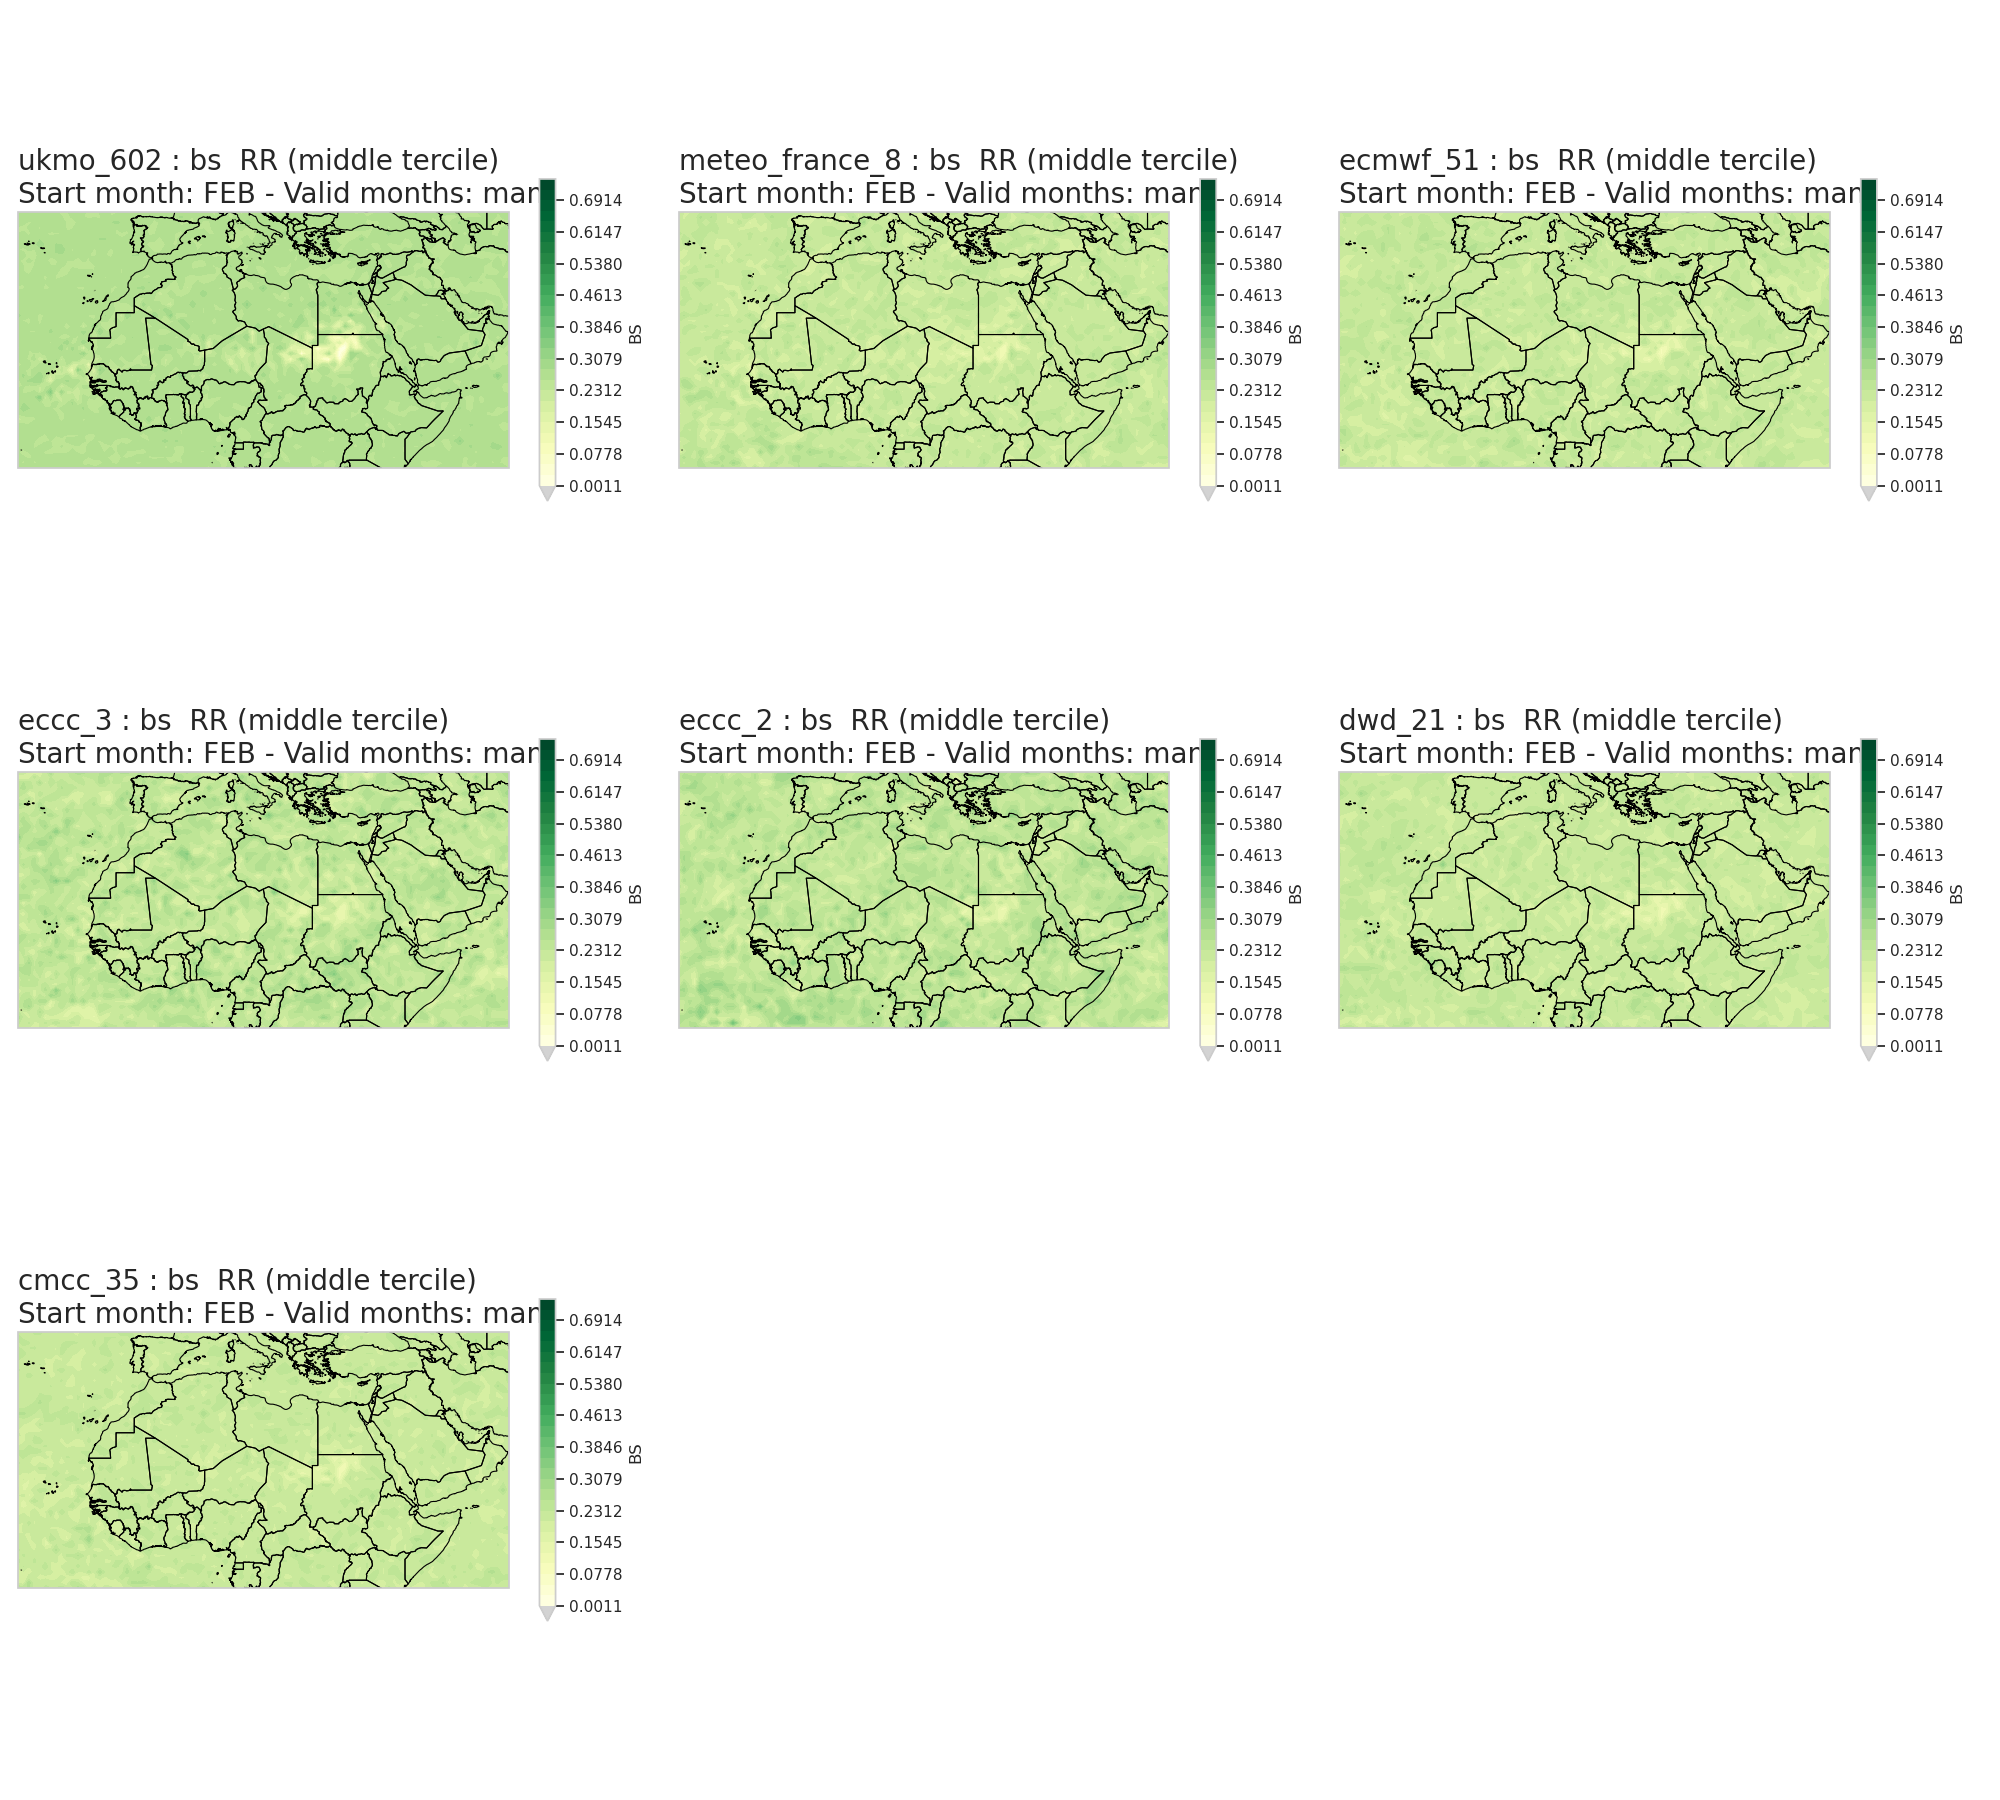
\includegraphics[scale=0.3]{plots/prob/bs/bs_mam_RR_middle.png}
\caption{3-months Rolling mean of Brier Score in MENA Region for all centers middle tercile MAM}
\end{figure}

the spacial distribution of the BS is homogeneous, the same performance across the MENA region, almost all centers perform well for all lead-times, for  tercile there is a little lower performance for the middle tercile.
Hint, for the other seasons the results are almost the same. 


\paragraph{focus on North Africa}:

there is no big difference in North Africa.
\vspace{1.5cm}
\paragraph{focus on Arabian Peninsula}:

there is no big difference in Arabian Peninsula.
\subsubsection{Reliability}

\begin{figure}[H]
    \centering
    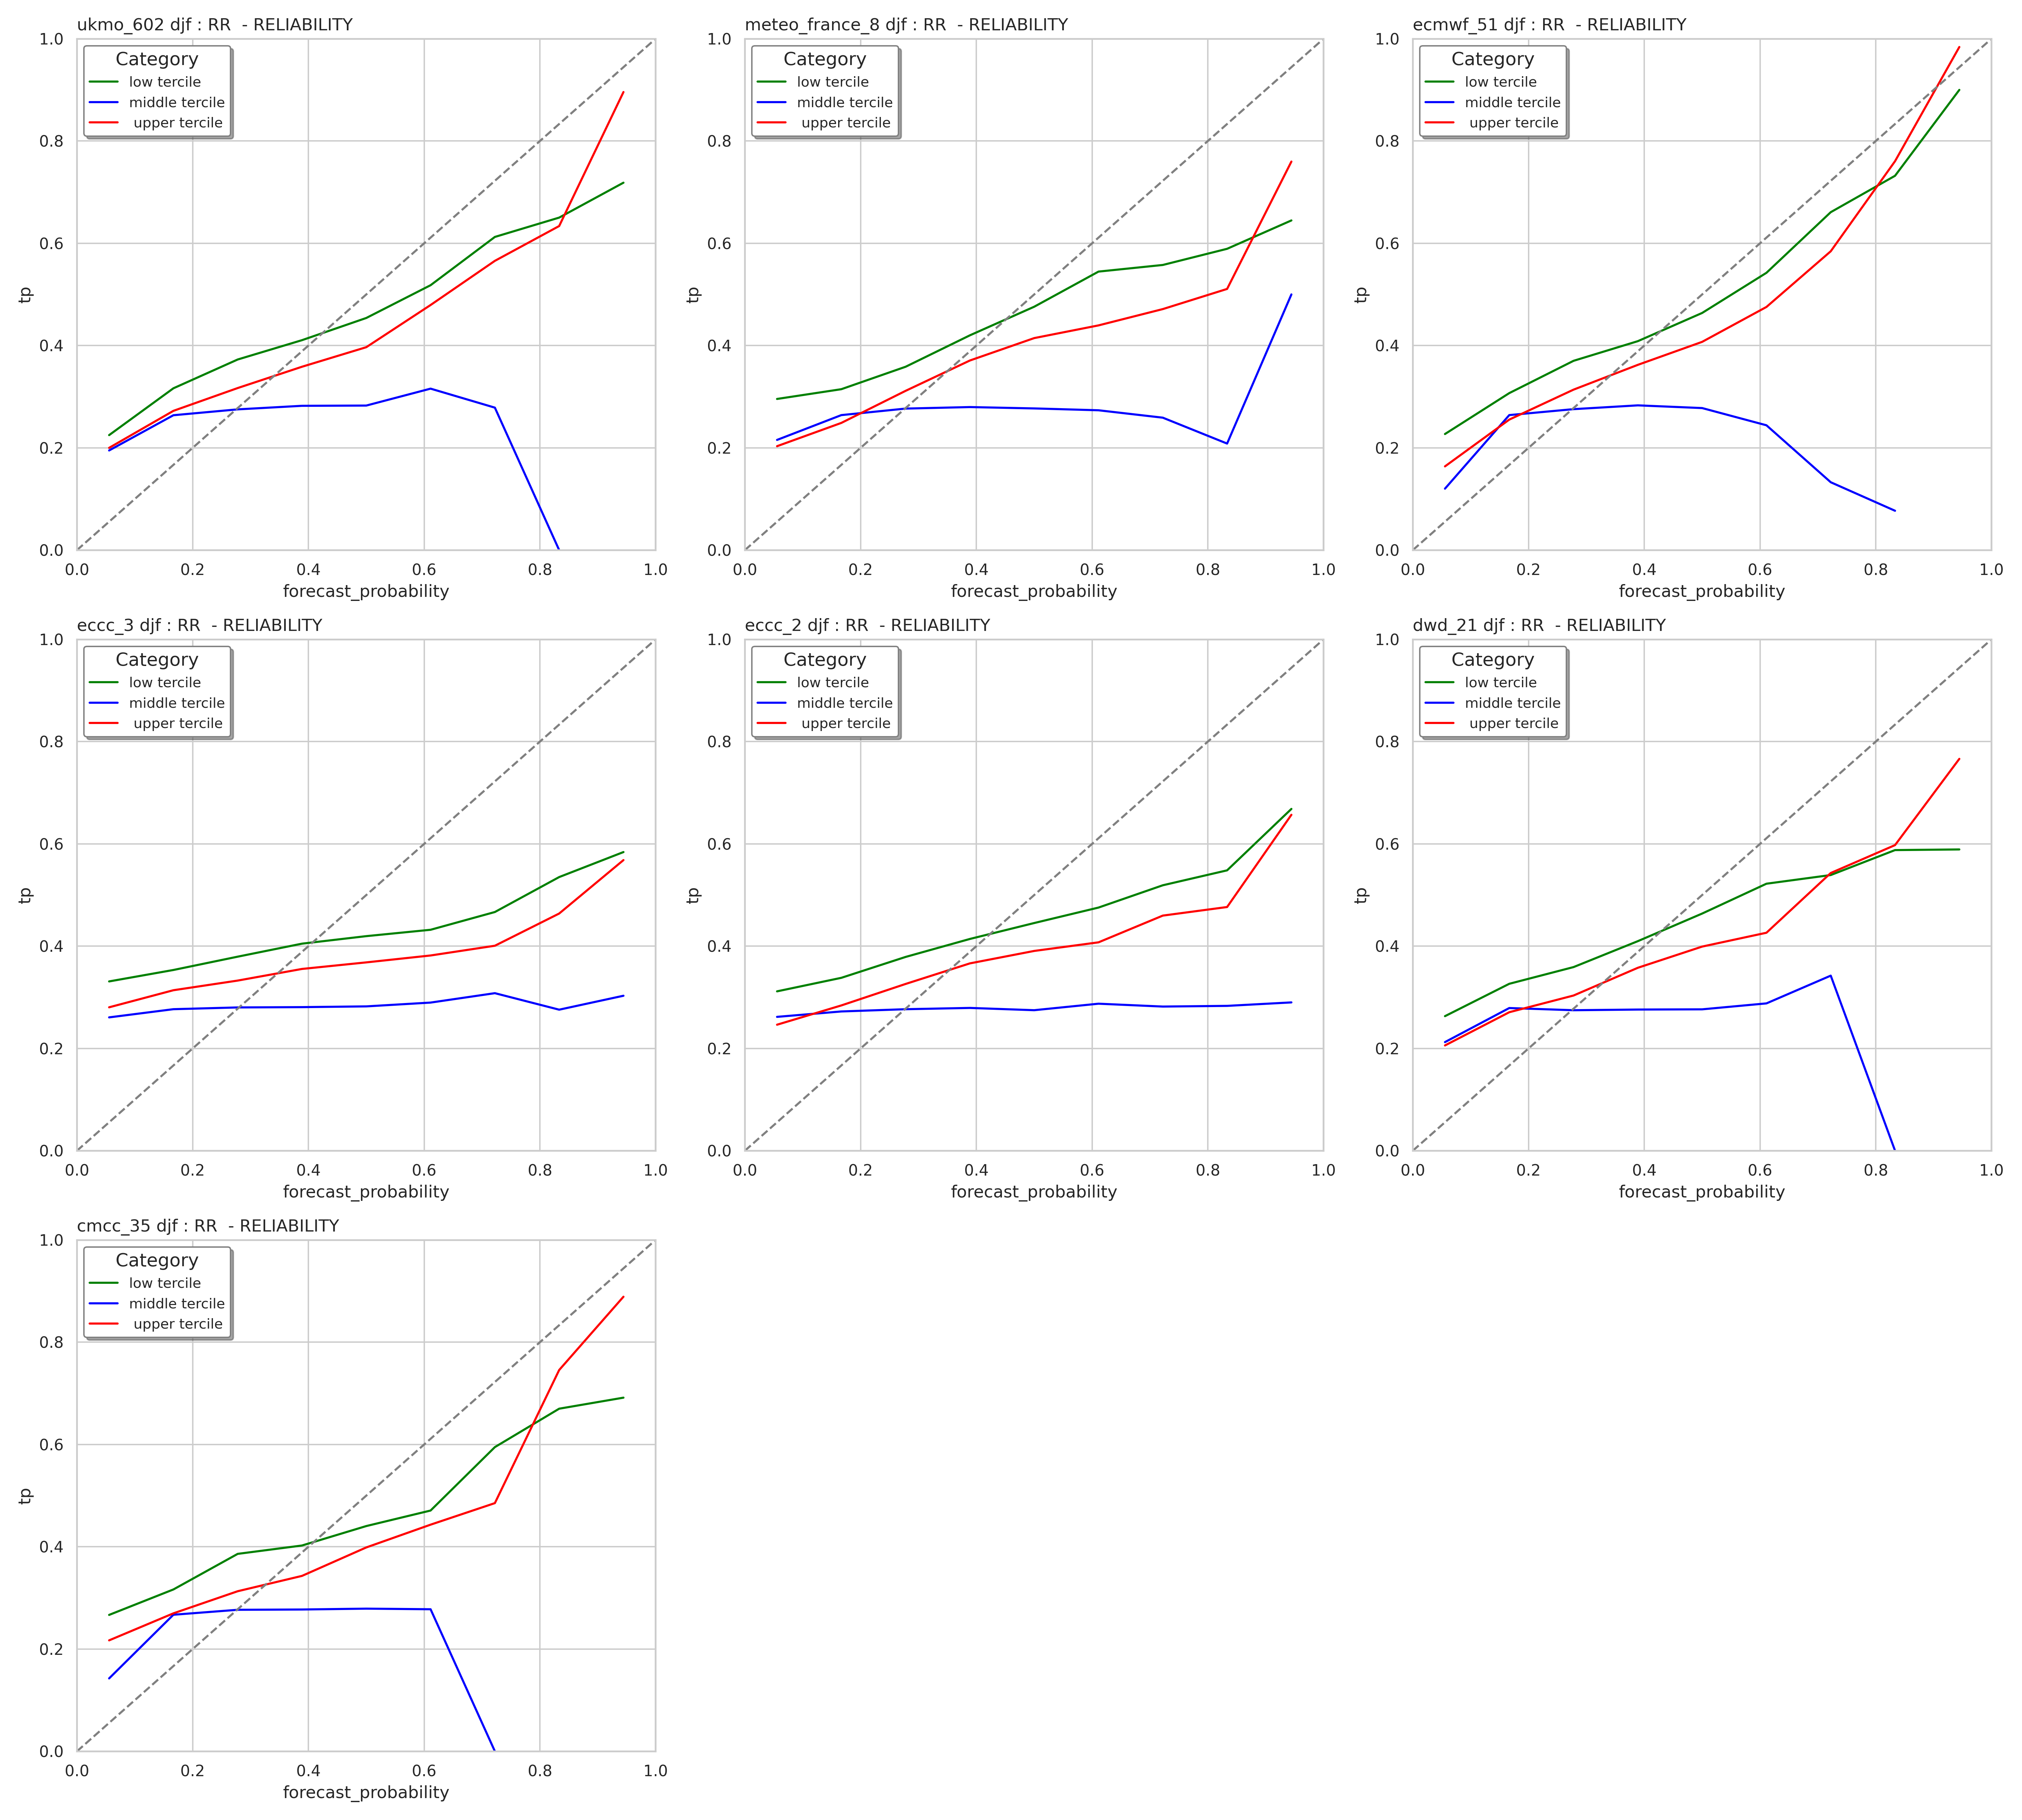
\includegraphics[scale=0.25]{plots/prob/rela/rela_diagram_djf_RR.png}
    \caption{The Reliability diagram  . \textbf{\textit{(45 degree for perfect reliability)}}}
\end{figure}

The reliability diagram for DJF, shows moderate performance, the \textbf{\textit{UKMO, ECMWF and CMCC-35}} have good performance especially for  upper and lower terciles, nevertheless, the performance for middle tercile is week for all centers.  

\begin{figure}[H]
    \centering
    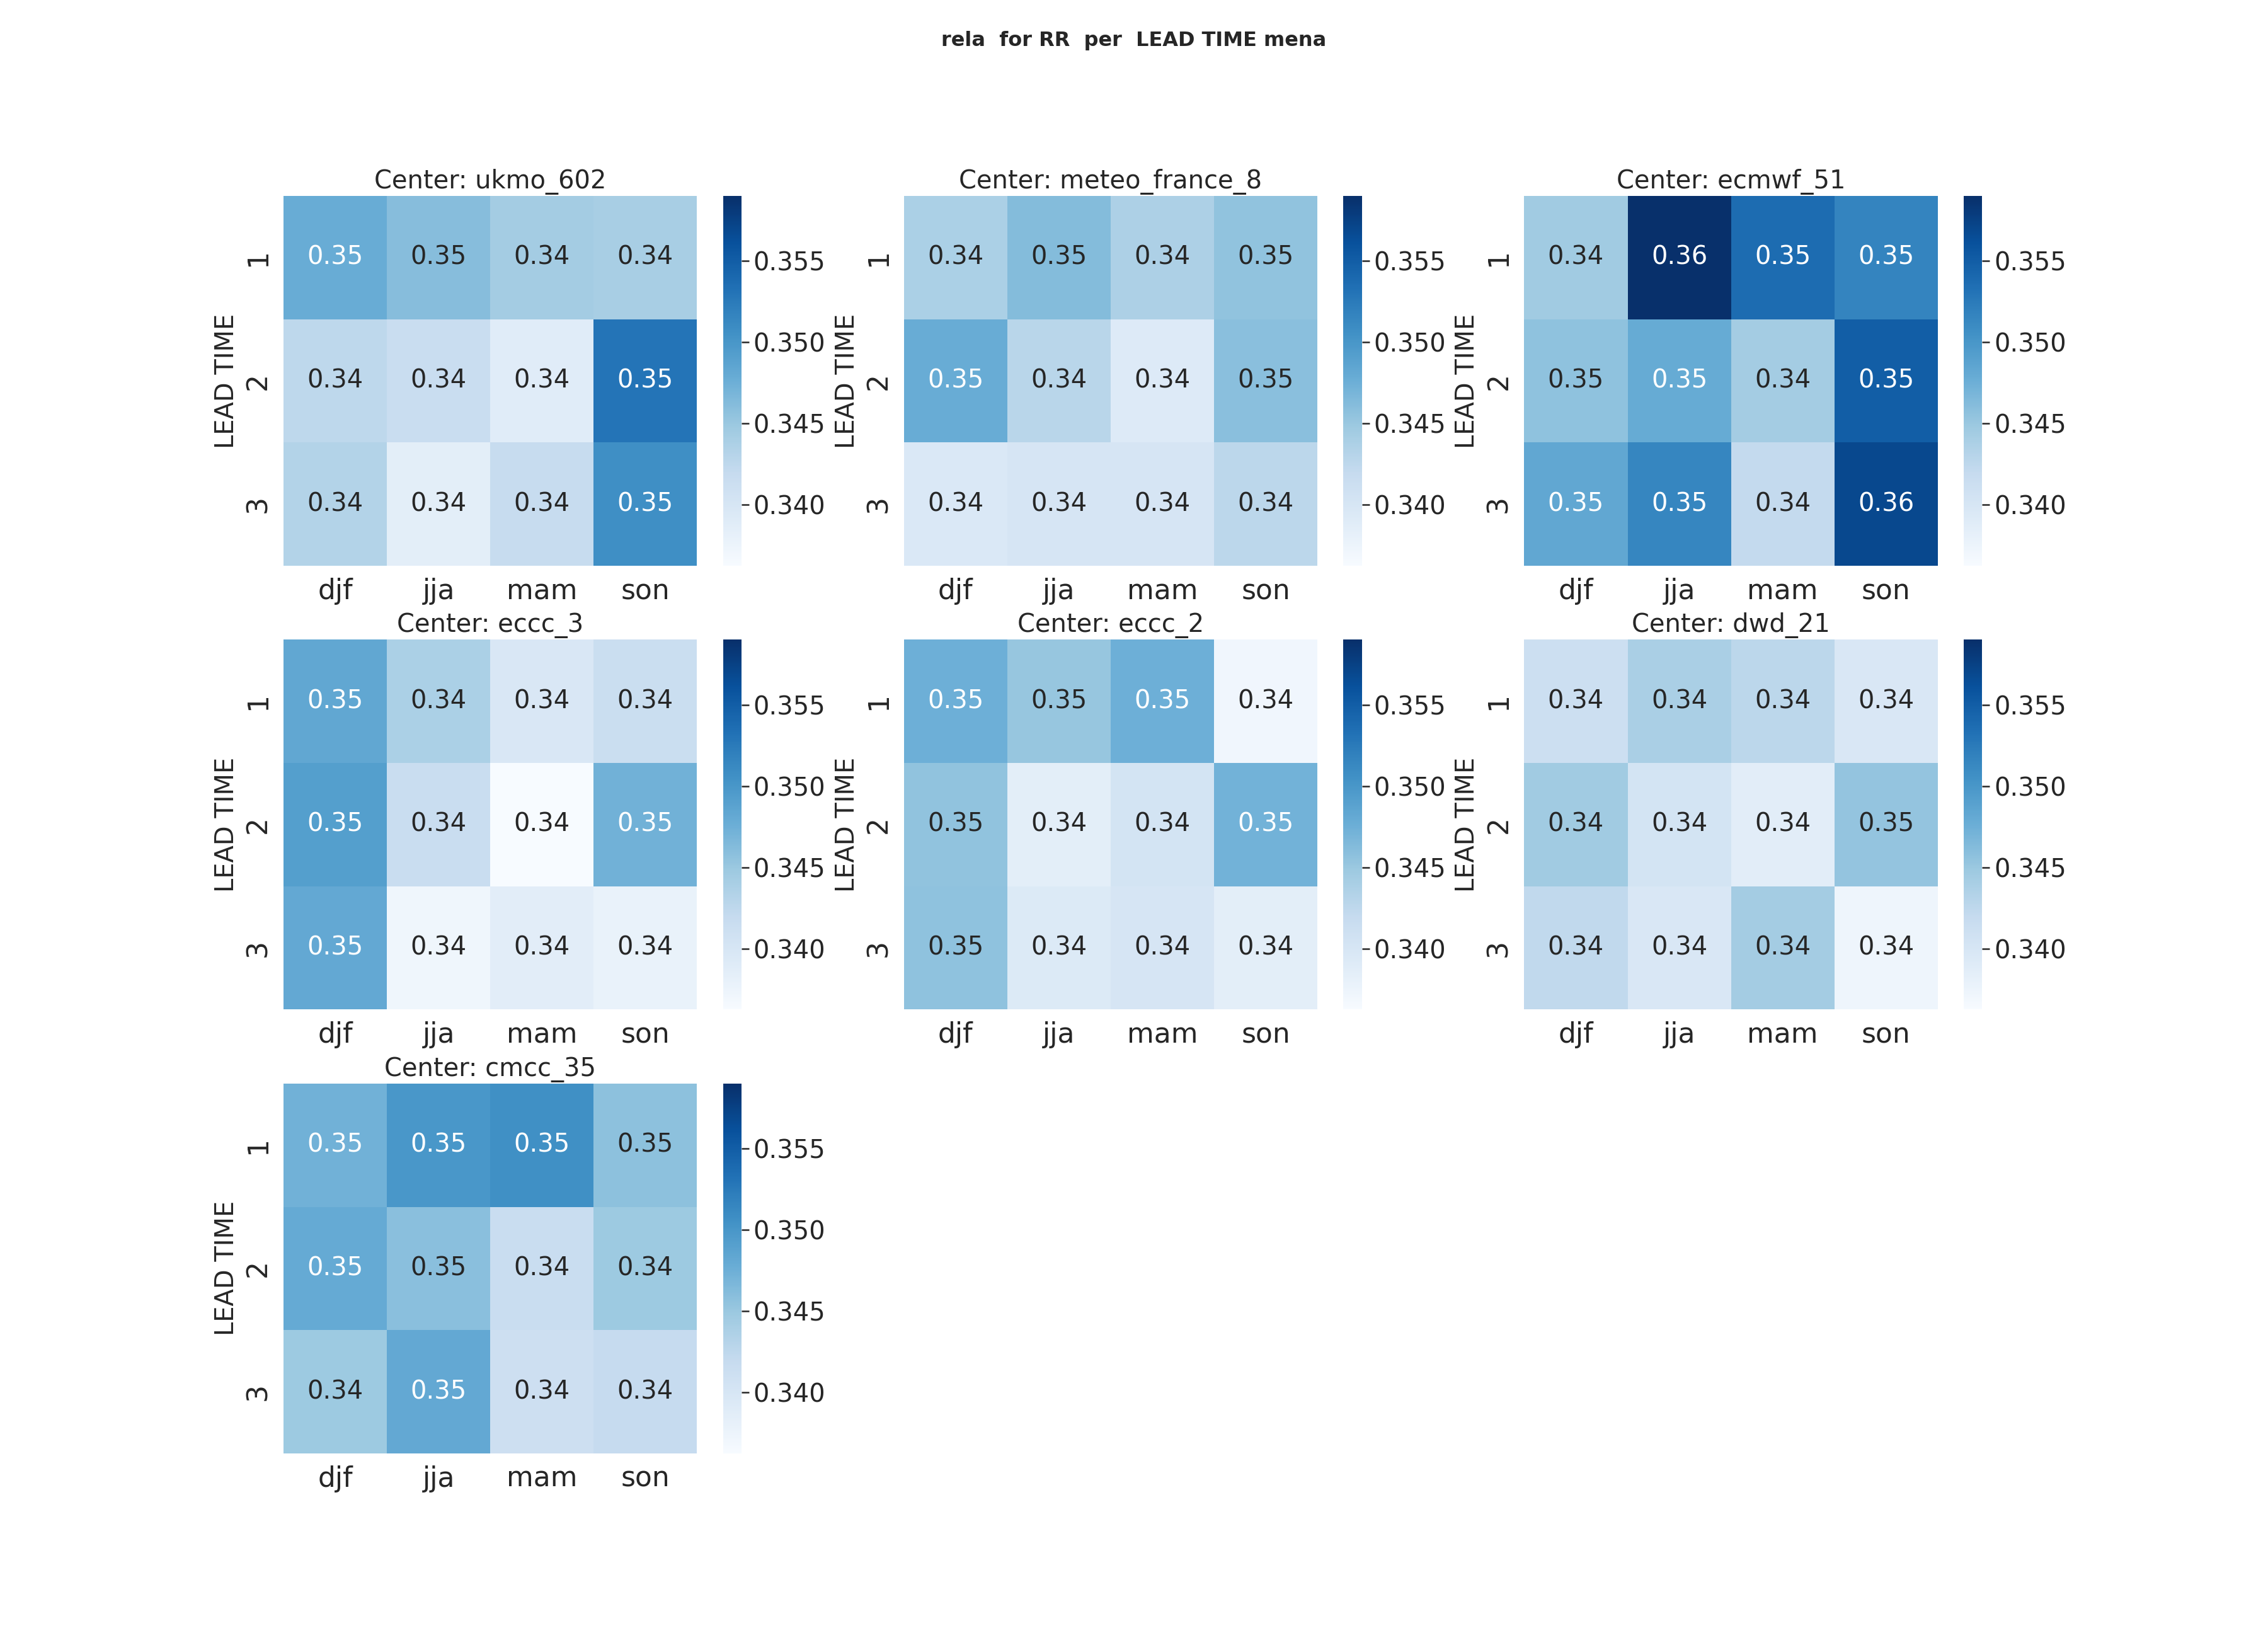
\includegraphics[scale=0.25]{plots/prob/rela/rela_RR_mena.png}
    \caption{The Reliability Score  . \textbf{\textit{(0 means perfect Reliability)}}}
\end{figure}

In the figure above, all centers demonstrate similar moderate performance in term of reliability. But deep analysis within the figure below, shows that all centers give similar description of the reliability, also the stability along lead-time is a good indicator despite of the moderate results (0.3), we can rely on all models  because of the acceptable results and the stability along time.
\paragraph{focus on North Africa}:

there is no big difference in North Africa.

\paragraph{focus on Arabian Peninsula}:




\begin{figure}[H]
    \centering
    \includegraphics[scale=0.25]{plots/prob/rela/rela_RR_ArabianPeninsula.png}
    \caption{The Reliability Score Arabian Peninsula . \textbf{\textit{(0 means perfect Reliability )}}}
\end{figure}

There is a little Decline in the reliability of the Arabian Peninsula, especially f\textbf{\textit{ECMWF}}



\subsubsection{The ranked probability score (RPS)}


\begin{figure}[H]
    \centering
    \includegraphics[scale=0.25]{plots/prob/rps/rps_RR_mena.png}
    \caption{The Heatmap of  RPS Score on MENA region for Precipitations    . \textbf{\textit{(0 means perfect RPS)}}}
\end{figure}

In the figure above, all centers demonstrate moderate performance, except for \textbf{\textit{ECCC}}, which shows noticeably lower performance. 


\begin{figure}[H]
    \centering
    \includegraphics[scale=0.25]{plots/prob/rps/rps_djf_RR.png}
    \caption{The   RPS Score on MENA region for Precipitations DJF . \textbf{\textit{(0 means perfect RPS)}}}
\end{figure}

the spacial distribution of the RPS, is homogeneous, in all the region the score is good for all centers.

\paragraph{focus on north africa:}

there is no big difference in North Africa.

\paragraph{focus on Arabian Peninsula}:

there is no big difference on Arabian Peninsula.


\subsubsection{Relative operating characteristics}

\begin{figure}[H]
    \centering
    \includegraphics[scale=0.25]{plots/prob/roc/roc_RR_category.png}
    \caption{The Heatmap of ROC Score for each category  . \textbf{\textit{(1 means perfect ROC)}}}
\end{figure}

In the figure above, it is clear that all forecasting centers show similar performance levels overall. However, the Middle Tercile consistently yields the lowest scores across all models. This finding is significant as it underscores the ability of all models to effectively predict extreme events, both above and below normal. In contrast, the models struggle more with predicting normal situations, which are inherently more difficult to forecast. The lower performance in the Middle Tercile highlights the challenge of accurately predicting conditions that are neither extreme nor easily distinguishable from typical climate variability. This suggests that while the models are proficient in forecasting extreme events, they face greater challenges when predicting more moderate, "normal" conditions.
\begin{figure}[H]
    \centering
    \includegraphics[scale=0.25]{plots/prob/roc/roc_RR_lead_time.png}
    \caption{The Heatmap of ROC Score for lead-times. \textbf{\textit{(1 means perfect ROC)}}}
\end{figure}

For the analysis per lead-time , all forecasting centers demonstrate similar and generally good performance. In most cases, the highest scores are observed for the first lead-time. However, an exception occurs during the SON (September-October-November) season, where the best performance is seen at the second lead-time. This variation suggests that while the models are consistently strong in the first lead-time, certain seasonal conditions, like those in SON, may benefit from a slightly longer forecast horizon to capture the full dynamics of the climate

\begin{figure}[H]
    \centering
    \includegraphics[scale=0.3]{plots/prob/roc/roc_son_RR_upper.png}
    \caption{The ROC Score Upper tercile SON    . \textbf{\textit{(1 means perfect ROC)}}}
\end{figure}


\begin{figure}[H]
    \centering
    \includegraphics[scale=0.3]{plots/prob/roc/roc_son_RR_middle.png}
    \caption{The ROC Score Middle tercile SON    . \textbf{\textit{(1 means perfect ROC)}}}
\end{figure}

The spatial distribution of the ROC score highlights an important finding. For precipitation, all centers demonstrate better performance in predicting the upper tercile, with similar results observed for the lower tercile. However, the performance in the middle tercile is considerably weaker, with high variability and lower scores, particularly in regions such as Egypt and Libya, where values are notably low. In this tercile, no significant differences are observed between the models, indicating a consistent struggle across all forecasting systems in dealing with moderate or normal precipitation events.

In contrast, the upper tercile displays some variability in the spatial distribution of scores, with the best performance seen in the Arabian Peninsula and parts of East Africa, particularly for the \textbf{\textit{ECMWF and UKMO}} models. This result underlines the models' relative strength in forecasting extreme precipitation events while emphasizing the challenges they face in predicting more moderate conditions.

				\paragraph{focus on north africa:}

there is no big difference in North Africa.
	
\paragraph{focus on Arabian Peninsula}:



\begin{figure}[H]
    \centering
    \includegraphics[scale=0.25]{plots/prob/roc/roc_RR_category_ArabianPeninsula.png}
    \caption{The ROC Score for each category Arabian Peninsula . \textbf{\textit{(1 means perfect ROC)}}}
\end{figure}


\begin{figure}[H]
    \centering
    \includegraphics[scale=0.25]{plots/prob/roc/roc_RR_lead_time_ArabianPeninsula.png}
    \caption{The average of  ROC Score on all categories for Arabian Peninsula . \textbf{\textit{(1 means perfect ROC)}}}
\end{figure}


For the roc score, the focus on Arabian Peninsula in category, show no big difference, as for the analysis along lead-time, there is a few improvement for DJF, MAM and SON, instead of JJA that shows low values for all centers. 																								
\subsubsection{Relative operating characteristics Skill Score}

In the figure above, the ECMWF exhibit the best performance for all terciles and periods. However, we should notice that the performance is very low for the middle tercile in all centers. For the analysis along time, the performance is so low, the best performance is in the first lead-time, except the SON which shows the best performance for the second lead-time. Above all, the \textbf{\textit{ecmwf}} shows the best performance.

\begin{figure}[H]
    \centering
    \includegraphics[scale=0.25]{plots/prob/rocss/rocss_RR_category.png}
    \caption{The ROCSS Score for each category  . \textbf{\textit{(1 means perfect ROCSS)}}}
\end{figure}


\begin{figure}[H]
    \centering
    \includegraphics[scale=0.25]{plots/prob/rocss/rocss_RR_lead_time.png}
    \caption{The average of  ROCSS Score on all categories    . \textbf{\textit{(1 means perfect ROCSS)}}}
\end{figure}



\begin{figure}[H]
    \centering
    \includegraphics[scale=0.3]{plots/prob/rocss/rocss_mam_RR_middle.png}
    \caption{The ROC Skill Score Middle tercile MAM . \textbf{\textit{(1 means perfect ROCSS)}}}
\end{figure}

\begin{figure}[H]
    \centering
    \includegraphics[scale=0.3]{plots/prob/rocss/rocss_mam_RR_upper.png}
    \caption{The ROC Skill Score Upper tercile MAM    . \textbf{\textit{(1 means perfect ROCSS)}}}
\end{figure}


The spatial distribution of the ROCSS indicates consistent performance across all forecasting centers for this score. However, the spatial patterns are not well-defined for both the upper and middle terciles. Notably, the middle tercile exhibits high spatial variability, with generally lower values compared to the other terciles. These findings align with the previously observed results for the ROC score, further confirming that forecasting performance is weaker and more inconsistent for the middle tercile. This underscores the ongoing challenge of accurately predicting moderate conditions, while extreme events are handled with greater reliability.


\paragraph{focus on north africa:}
\begin{figure}[H]
    \centering
    \includegraphics[scale=0.25]{plots/prob/rocss/rocss_RR_category_NorthAfrica.png}
    \caption{The ROCSS Score for each category North Africa . \textbf{\textit{(1 means perfect ROCSS)}}}
\end{figure}


\begin{figure}[H]
    \centering
    \includegraphics[scale=0.25]{plots/prob/rocss/rocss_RR_lead_time_NorthAfrica.png}
    \caption{The average of  ROCSS Score on all categories North Africa   . \textbf{\textit{(1 means perfect ROCSS)}}}
\end{figure}


the rocss for North Africa is in general lower, thus the performance is less accurate.

\paragraph{focus on Arabian Peninsula}:
\begin{figure}[H]
    \centering
    \includegraphics[scale=0.25]{plots/prob/rocss/rocss_RR_lead_time_ArabianPeninsula.png}
    \caption{The average of  ROCSS Score on all categories for Arabian Peninsula . \textbf{\textit{(1 means perfect ROCSS)}}}
\end{figure}


the rocss for Arabian Peninsula is in general lower, thus the performance is less accurate.

\subsubsection{summary}
\begin{table}[h!]
\centering
\begin{tabularx}{\textwidth}{@{}p{2.5cm}p{4cm}p{4cm}p{2.5cm}p{3cm}@{}}
\toprule
\textbf{Metric}       & \textbf{Focus}                                    & \textbf{What it Measures}                         & \textbf{Dependent on Observed Outcomes?} & \textbf{Visualization/Tools}             \\ \midrule
\textbf{Reliability}   & Probabilities match observed frequencies          & Calibration of probabilities                      & Yes                                      & Reliability diagram                      \\
\textbf{Discrimination} & Differentiating between outcomes                 & Ability to distinguish events from non-events    & Yes                                      & ROC curve, AUC                           \\
\textbf{Sharpness}     & Boldness of probabilities (away from average)     & Confidence of the forecast                        & No                                       & Histogram of forecast probabilities      \\
\textbf{Resolution}    & Informativeness and variability of forecast       & Ability to provide specific, useful info         & Yes                                      & Brier Score decomposition                \\ \bottomrule
\end{tabularx}
\caption{Key differences between reliability, discrimination, sharpness, and resolution in seasonal forecasting.}
\end{table}

\newpage
\thispagestyle{empty}
\mbox{}

\endinput